% it is part of
% TUDa-CI -- Corporate Design for TU Darmstadt
% ----------------------------------------------------------------------------
%
% Copyright (C) 2018--2025 by Marei Peischl <marei@peitex.de>
%
% ============================================================================
% This work may be distributed and/or modified under the
% conditions of the LaTeX Project Public License, either version 1.3c
% of this license or (at your option) any later version.
% The latest version of this license is in
% http://www.latex-project.org/lppl.txt
% version 2008/05/04 or later.
%
% This work has the LPPL maintenance status `maintained'.
%
% The current maintainer of this work is
%   Marei Peischl <tuda-ci@peitex.de>
%
% The development repository can be found at
% https://github.com/tudace/tuda_latex_templates
% Please use the issue tracker for feedback!
%
% If you need a compiled version of this document, have a look at
% http://mirror.ctan.org/macros/latex/contrib/tuda-ci/doc
% or at the documentation directory of this package (if installed)
% <path to your LaTeX distribution>/doc/latex/tuda-ci
% ============================================================================
%
% !TeX program = lualatex

% Enable PDF/A via pdfmanagement (recommended)
\DocumentMetadata{
  pdfstandard={a-2b},
  pdfversion=1.7,
  lang=en,
}

\documentclass[
  english,
  accentcolor=2d,
  ruledheaders=section,
  class=report,
  thesis={type=master},
  fontsize=11pt,
  parskip=half,
  custommargins=false,
  marginpar=false,
  pdfa=true % Hinweis: wird bei \DocumentMetadata i. d. R. ignoriert
]{tudapub}

%%%%%%%%%%%%%%%%%%%
% Language setup
%%%%%%%%%%%%%%%%%%%
\usepackage[main=english, german]{babel}

%%%%%%%%%%%%%%%%%%%
% Typography & utils
%%%%%%%%%%%%%%%%%%%
% we already have booktabs/array loaded; no extra packages needed

\usepackage{microtype}
\usepackage[autostyle]{csquotes} % \enquote
\usepackage{xurl}   
\usepackage{dsfont}

% --- TikZ & PGF ---
\usepackage{tikz}
\usetikzlibrary{positioning} % für "below=of ..." und "right=of ..."
\usetikzlibrary{calc}        % für Koordinaten-Berechnungen ($(a)+(x,y)$)
\usetikzlibrary{arrows.meta} % für Pfeilspitzen wie ">=Stealth"
\usetikzlibrary{shapes.misc} % falls du rounded corners etc. nutzt
\usetikzlibrary{fit}         % nur wenn du fit nodes benutzt
\usetikzlibrary{backgrounds} % optional, für Ebenen (nicht zwingend)

% --- Farben (falls nicht schon geladen) ---
\usepackage{xcolor}

% --- deine Node Styles (box, op, note, streamText, streamLIWC etc.) ---
% Falls du die noch nicht global definiert hast, brauchst du sowas:
\tikzset{
  box/.style={draw, thick, rounded corners, align=center, inner sep=3pt},
  op/.style={draw, thick, rectangle, align=center, rounded corners=1pt,
             fill=gray!5, inner sep=3pt},
  note/.style={align=left, font=\footnotesize, text=black!60},
  streamText/.style={draw=blue!60!black, text=blue!60!black},
  streamLIWC/.style={draw=violet!70!black, text=violet!70!black},
}           %

%%%%%%%%%%%%%%%%%%%
% Figures & tables
%%%%%%%%%%%%%%%%%%%
\usepackage{graphicx}
\graphicspath{{figures/}}        % Bilder im Ordner "figures/"
\usepackage{float}               % für [H]
\usepackage{subcaption}
\captionsetup[sub]{font=small}

\usepackage{booktabs}
\usepackage{ragged2e} % stellt \RaggedRight bereit

\usepackage{array}
\usepackage{longtable}
\usepackage{pdflscape}
\setlength{\LTcapwidth}{\textwidth} % Captionbreite für longtable
\usepackage{multirow}
\usepackage[section]{placeins}   % Floats nicht über Section hinaus

%%%%%%%%%%%%%%%%%%%
% Math
%%%%%%%%%%%%%%%%%%%
\usepackage{amsmath}
\usepackage{amssymb}

%%%%%%%%%%%%%%%%%%%
% Misc
%%%%%%%%%%%%%%%%%%%
\usepackage{comment}
\usepackage{makecell}

%%%%%%%%%%%%%%%%%%%
% Bibliography
%%%%%%%%%%%%%%%%%%%
\usepackage[style=ieee,backend=biber, citestyle=numeric-comp, giveninits= true, maxnames= 6, minnames =1, doi = true, url = true, isbn = false, eprint= false]{biblatex}
\addbibresource{literature.bib}

%%%%%%%%%%%%%%%%%%%
% Meta
%%%%%%%%%%%%%%%%%%%
\title{Master Thesis: Fusion of transformer-based language representations with psycholinguistic LIWC features for improved detection of cybergrooming in chat logs}
\author{Amelie Oberkirch}
\reviewer{Prof. Dr. Martin Steinebach \and Shiying Fan}

% The following elements will be placed on the title page
\department{inf}% If defined the shorthand will be replaced by the full name otherwise it's used directly.
\institute{Fraunhofer-Institut für Sichere Informationstechnologie}
\group{Media Security}

\submissiondate{13. October 2025}

%\tuprints{urn=XXXXX,printid=XXXX,year=2022,license=cc-by-4.0}% License information for TUprints

\begin{document}

\maketitle
\affidavit[
signature=Amelie Oberkirch,
signature-image={
\includegraphics[width=\width]{bildschirmfoto.png}}]

\chapter*{Acknowledgements}
\addcontentsline{toc}{chapter}{Acknowledgements}

\begin{center}
  \begin{minipage}{0.85\linewidth}
    \itshape
    I would like to thank my supervisor Shiying for her guidance and support throughout this work.

    Thank you to Leon, Jonas and Lukas, whose commitment and daily companionship in the library provided both motivation and encouragement during the last months.

   I would also like to thank Lena and Franzi for their continuous encouragement and friendship and Alba, Lara, and Leon, for being my supportive home environment during this period.

    And finally thank you to Jan and my family, whose encouragement and constant support have been indispensable throughout this journey.
  \end{minipage}
\end{center}

\chapter{Abstract}

In today's digital age, cybergrooming poses a dangerous threat to the lives of children and young people and requires automatic technologies with high detection performance to support child protection. This work analyzes the integration of LIWC-2022 features \cite{pennebaker2022liwc} into BERT representations \cite{devlin2019bert} using a cross-attention-based feature fusion approach. The goal is to improve detection performance, while also enhancing explainability by identifying relevant LIWC features contributing to the model's decisions. On the basis of a dataset consisting of complete conversations from 605 identified sexual predators collected by the Perverted Justice Foundation and the  non-grooming dialogues by PAN12 \cite{inches2012pan}, a BERT baseline was created, which was additionally secured against domain and length leakage using synthetic data. Afterwards, the feature-fusion model was evaluated using two different LIWC-2022 feature sets. The first set included all 118 LIWC features, while the second set focused on a subset of 49 psychometric LIWC features that have been highlighted in the literature as relevant for manipulative communication in grooming chats. The results show, that feature fusion increased the F1 score by 1.7\% to 98.7 \% using both kind of feature sets where especially the precision increased leading to a lower rate of false positives. In addition to the feature-fusion evaluation, an analysis of the differences between grooming and non-grooming conversations was conducted using LIWC features, revealing strong differences in categories like cognitive processes, social processes and temporal orientation. Furthermore, SHAP \cite{lundberg2017shap} explainability analysis was performed to identify the most relevant LIWC features contributing to the model's decisions. The SHAP analysis revealed that LIWC features contribute to a percentage of around 9.66\% when using the full LIWC feature set and about 7.41\% for the psychometric subset to the model's predictions. Also, the SHAP analysis confirmed the relevance of the LIWC features related to cognitive and social processes when using the psychometric subset. Overall, this work highlights the potential of hybrid models that combine semantic understanding with psycholinguistic insights to better identify cybergrooming behavior in online communication.

%%% Überarbeitet

%% The affidavit was deactivated by default at the request of Department II.
%% According to the department, the legally binding text can be found at
%% https://www.tu-darmstadt.de/studieren/studierende_tu/studienorganisation_und_tucan/hilfe_und_faq/artikel_details_de_en_37824.de.jsp
%% The docx file should be used, printed out, signed, scanned and then integrated.
%% The easiest way to do this is to use the pdfpages package.
%%
%% For compatibility reasons for the other templates, the function is still available.
%% \affidavit[
%%   signature-image={\includegraphics[width=\width,height=1cm]{example-image}},
%%   % <there may be additional options here>
%% ]

\tableofcontents
\listoffigures
\listoftables
% Optional:
% \listoffigures
% \listoftables


\chapter{Introduction} 



\begin{comment}
    So ist es das Ziel von Oberkirch (2025), sprachliche Embeddings von DeBERTa v3 mit LIWC-basierten psychometrischen Features zu kombinieren, um die Erkennungsleistung zu steigern und gleichzeitig die Vorhersagen besser erklärbar zu machen. Konkret wird ein zweistufiges Modell aufgebaut: Zunächst feintuned man DeBERTa auf den segmentierten Chats, extrahiert dann pro Segment einen Feature-Vektor aus LIWC-Kategorien (z. B. Werte für Emotion, Kognition, soziale Prozesse etc.), und fügt beide Vektoren zusammen, um sie gemeinsam einem Klassifikator zuzuführen. Erste Experimente zeigen, dass diese Feature-Fusion die Erkennungsgenauigkeit verbessert und Aufschluss darüber geben kann, welche psychologischen Signale der Grooming-Kommunikation vom Modell genutzt werden. Insgesamt gelten hybride Modelle, die linguistisches Kontextverständnis eines großen Sprachmodells mit psycholinguistischen Indikatoren verknüpfen, als Best Practice, um subtile manipulative Strategien besser zu erkennen. Sie ermöglichen es zudem, die Entscheidungen des Modells inhaltlich zu interpretieren (etwa wenn hohe Werte in LIWC–Angst oder LIWC–Sexualität zum Ausschlag für eine Klassifizierung beitragen).
\end{comment}


% Hier könntest du ein paar saubere Statistiken einbringen
In today's world, social media are an integral part of the lives of children and young people and offer extensive opportunities for global networking and the exchange of ideas. In addition to the great potential of the latest technologies, social media also pose many dangers, especially for children and young people. Cybergrooming represents a significant danger in this regard - whereby minors are often contacted and emotionally influenced by adults using communicative manipulation in order to initiate or prepare sexual contact.
% Motivation, Problemstellung, Zielsetzung, Forschungsfrage, Aufbau der Arbeit



\chapter{Related Work}

This chapter introduces the term “cybergrooming” and relevant research in the field of cybergrooming and cybergrooming detection. The first section provides an overview of the psychological and communicative dynamics of cybergrooming. The second section additionally focuses on technical approaches to detecting grooming behavior in online conversations, with an emphasis on machine learning methods and their integration with psycholinguistic features.

%%% Überarbeitet

\section{Understanding Cybergrooming}


The terms “online grooming” and “cybergrooming” are often used synonymously to describe the process by which an adult establishes a digital relationship with a minor in order to achieve and facilitate subsequent sexual exploitation. In academic literature, “online grooming” is the internationally established term for this phenomenon, particularly in the fields of psychology, criminology and child protection. However, the synonymous term “cybergrooming” is more commonly used in media education and German-language legal discourse, with an emphasis on the technological environment in which the grooming takes place \parencite{mladenovic2021cyber, schittenhelm2024cybergrooming}. \textbf{To maintain terminological clarity, the term “cybergrooming” is used throughout this thesis. } %Überarbeitet 

Cybergrooming can be seen as a psychological manipulation process in which a perpetrator uses digital communication technologies to befriend a minor, initiate sexual interactions online and/or arrange a physical meeting with the aim of sexual abuse \parencite{webster2021european}. This process usually takes place in several stages, in which trust is gradually built up, emotional dependence is created and the minor is desensitized to sexual content or requests \parencite{whittle2013review}. Groomers often present themselves as friendly and understanding, using engaging and emotionally supportive language rather than openly deceiving \parencite{broome2020psycholinguistic}. This process is facilitated by digital media, which allow perpetrators to remain anonymous and gain unrestricted access to children without direct adult supervision \parencite{mladenovic2021cyber}. %Überarbeitet


It is important to note that online grooming does not refer to the sexual abuse itself, but rather to the preparatory phase and psychological manipulation. The perpetrator uses targeted strategies to influence the victim's thoughts, emotions and decision-making processes in such a way that they serve his own intentions \parencite{schittenhelm2024cybergrooming}. This grooming dynamic is not limited to online contexts. The broader term “grooming” refers to any deliberate strategy used by perpetrators to emotionally condition and exploit defenseless minors and is a significant mechanism in cases of sexual abuse \parencite{craven2006grooming}.

While there is agreement on the manipulative nature of cybergrooming, researchers have developed various models to represent its dynamics, communication strategies and stages of development\parencite{kloess2014online}. These models have been proposed to conceptualize the process of cybergrooming and often describe it as a multi-stage process involving various phases such as friendship formation, relationship building, exclusivity, risk assessment, sexual interaction and conclusion. Importantly, research suggests that these phases do not necessarily occur in a fixed or linear order and that perpetrators may skip phases, return to earlier phases, or adapt their strategies depending on the victim and context. For example, Black et al.\ \parencite{black2015linguistic} conducted a qualitative content analysis of Facebook chat logs and identified linguistic patterns characteristic of different phases of grooming, providing empirical evidence for the nonlinear nature of the grooming process. 

To illustrate different conceptual approaches and understand the grooming process, the following section focuses on two well-known models: O'Connell's stage-based framework and Gupta's linguistic profiling approach. %%Überarbeitet




\section{Stages of Cybergrooming}

A key feature of grooming is its gradual and often strategically planned progression. Many studies describe grooming not as a one-time event, but as a multi-phase communication process in which perpetrators consciously build trust, establish emotional bonds and gradually introduce sexual content. The following studys illustrate this process using various phase models based on annotated chat logs. Despite their theoretical relevance, however, the empirical generalizability of these models remain controversial.

A frequently cited model comes from \textcite{oconnell2003typology}, who identified six consecutive phases: \emph{friendship building}, \emph{relationship building}, \emph{risk assessment}, \emph{exclusivity}, \emph{sexuality} and \emph{conclusion}. These phases form a kind of “linear roadmap” for the grooming process. The communication strategies of the phases range from small talk and compliments to risk assessments and explicit sexual innuendo or appointments. Although O'Connell's model has greatly influenced the conceptual understanding of grooming dynamics, it has been criticized for its limited empirical basis. For example, \textcite{broome2020psycholinguistic} and \textcite{LorenzoDus2019} point to methodological ambiguities regarding sample size, perpetrator demographics and the structural characteristics of the conversations analyzed. %%approved

Furthermore, the assumption of a fixed sequence has been challenged by subsequent empirical findings suggesting that grooming often develops not linearly but with overlapping or cyclical phases \parencite{Joleby2021offender}. Recent sequence analyses show that perpetrators often use trust-building measures, sexualization and risk assessment in parallel rather than in a strict sequence \parencite{Ringenberg2024assessing}.

An alternative, linguistically based model was proposed by \textcite{lorenzo2016understanding}. Based on the analysis of 24 chat logs from the online archive Perverted-Justice.com, the authors divide grooming into three dynamic phases: \emph{access}, \emph{approach} and \emph{entrapment}. In the entrapment phase in particular, linguistic strategies often overlap, making it difficult to draw clear boundaries between the phases. The authors identify four communication processes: deceptive trust development, sexual gratification, isolation and compliance testing. These are realized through strategic language use, such as praise, desensitization and personal disclosures. Politeness strategies in particular play a central role in manipulating the victim by simultaneously signaling control and trust. However, despite its depth, the study remains limited in its generalizability as it relies on a purely qualitative methodology and is based on lure chats with adult volunteers. More recent work shows that lure chats differ significantly from real victim interviews in key aspects such as threats, coercion and intensity of risk questioning \parencite{Ringenberg2024assessing}.  %%% approved

Another influential model was developed by \textcite{williamsmodel}, who analyzed convicted sex offenders in New Zealand. Their three-stage typology—\emph{relationship building}, \emph{sexual content} and \emph{assessment}—emphasizes the dynamics of early manipulation. According to \textcite{williamsmodel}, in the \emph{relationship building} phase, offenders adapt their language to that of adolescents in order to create a feeling of closeness. The \emph{sexual content} phase often begins subtly, for example through games or advice and ends with explicit offers. The \emph{assessment} phase serves to continuously evaluate risk and create an emotional profile of the victim.

A psychologically based extension is also provided by Olson's \emph{Luring Communication Theory} (LCT), which was originally designed for offline grooming but can also be applied to online contexts \parencite{Cano2014}. This model comprises three phases containing \emph{Deceptive Trust Development}, \emph{Grooming} and \emph{Physical Approach}. In the first phase, an emotional connection is established through personal exchange. This is followed by increasing sexualized communication, which finally transitions into a phase in which physical contact is initiated.

Taken together, these models show that grooming processes often proceed in strategically structured phases that are realized linguistically through specific communicative actions. %%Überarbeitet

\section{Towards Automated Detection of Online Grooming}

The sheer volume of modern online communication makes manual monitoring of cybergrooming in online chats, social media and online games virtually impossible. Automated detection systems are therefore essential for filtering and categorizing suspicious dialogues in real time. \cite{hamm2025llms}
To support timely detection and reduce the burden on victims, current research is increasingly focused on developing automated systems capable of detecting grooming behavior in online conversations. These systems aim to flag suspicious interactions in real time or near real time, enabling efficient protective measures in digital environments.

Over the past decade, a variety of approaches have emerged that rely on classical machine learning, the extraction of linguistic and behavioral features and modern deep learning techniques. Broadly speaking, these approaches to cybergrooming can be divided into three main paradigms: (1) \textit{Identification of sexual predators}, where the goal is to classify entire conversations as grooming or non-grooming; (2) \textit{Modeling the grooming process}, where the focus is on identifying the phases and strategies of grooming; and (3) \ Early detection of grooming, with the goal of identifying harmful intentions in the earliest stages of communication. The following sections present studies from each of these areas, highlighting their methodology, datasets and key findings. %%% Überarbeitet

\subsection{Sexual Predator Identification}
Villatoro-Tello et al. proposed a two-stage framework specifically aimed at identifying sex offenders who engage in grooming behavior in online chat environments \parencite{villatoro2012two}. Their approach first filters suspicious conversations based on lexical, stylistic and emotional characteristics and then classifies individual messages according to different grooming phases. Based on the PAN12 dataset for identifying sexual offenders, their model captures the sequential and manipulative nature of offenders' communication. Broome et al. supported this approach and conducted a comprehensive review of machine learning methods for identifying sex offenders \parencite{broome2020psycholinguistic}. They confirmed that the most effective approaches are based on linguistic features and emphasized the growing importance of deep learning models. In particular, they highlight models that can capture contextual and temporal dependencies. Both studies underscore the value of stage-aware and linguistic modeling in the development of robust systems for detecting grooming, while also pointing to the ethical necessity of transparency and explainability in high-risk applications. %%Überarbeitet


\subsection{Grooming Process Modeling}


The understanding of cybergrooming as a sequential and manipulative process has led to many efforts to model its phases. For example, Gupta et al. conducted one of the earliest qualitative studies, using the Perverted Justice dataset to analyze grooming behavior in chat logs \parencite{gupta2012characterizingpedophileconversationsinternet}. They based their work on O'Connell's six-phase model and manually labeled the perpetrators' messages accordingly. Their findings underscored the structured nature of grooming strategies and laid important groundwork for subsequent modeling efforts. %%Approved

Building on this foundation, Cano et al. operationalized Olson's Luring Communication Theory by defining three grooming phases themselves: Deceptive Trust Development, Grooming and Seeking Physical Approach \parencite{Cano2014}. They used linguistic, psycholinguistic and discourse-based features, including LIWC and sentiment analysis, to classify messages into the three phases using SVMs. Their results showed that discourse features were particularly effective in describing the progression of grooming behavior.  %% Approved

Furthermore, Black et al. emphasized the nonlinear and dynamic nature of grooming, highlighting that perpetrators often skip, repeat, or adapt phases depending on context and interpersonal factors \parencite{black2015linguistic}. This finding underscores the importance of process-based modeling over static classification. %% Approved

%% Überarbeitet

\subsection{Early Grooming Detection}


Efforts to detect grooming at an early stage often focus more on classifying individual messages rather than entire conversations. One such approach is presented by Isaza et al., who developed a CNN-based model trained on the PAN12 dataset to classify short messages as grooming or non-grooming \parencite{Isaza2022classifying}. Their architecture utilizes semantic features through pre-trained word embeddings (Word2Vec) and applies convolutional filters of various sizes to detect n-gram-like patterns. Although the model achieved a high recall rate, it suffered from low precision due to class imbalance. Nevertheless, it proved useful for early intervention as it correctly marked a large number of true positives.  % Approved

Another relevant contribution comes from \textcite{schlaepfer2022online}, which dealt with machine learning methods for the early detection of sex offenders in online chats. Using pre-trained language models and ensemble classifiers, their approach focused on identifying grooming behavior at the conversation level. Although their work did not involve manual annotation at the message level, it showed that linguistic signals embedded in early parts of conversations can be used to distinguish chats from sex offenders from harmless chats. Their findings underscore the potential of automated systems to detect grooming attempts in their early stages and contribute to the development of real-time safety measures. %%approved

%%Überarbeitet

\subsection{Machine Learning Approaches}

While early research focused on the classification of perpetrators and the modeling of phases, modern work reflects a broader methodological field, often motivated by the need for scalable and interpretable detection systems. In their systematic review, An et al. \ \parencite{an2025cybergrooming} emphasize that machine learning approaches play a central role in the automated detection of grooming, particularly due to their ability to process large amounts of online text. However, they caution that most systems remain purely reactive and lack integration with social science insights into the dynamics of grooming. To close this gap, hybrid models are needed that combine the statistical power of machine learning with insights from psychology and criminology.

From this perspective, Gunawan et al. \ \parencite{gunawan2016detecting} investigated behavioral indicators by training a classifier on the Perverted Justice dataset. Features such as message length, conversation turns and response time were used to capture conversation flow. Their results suggest that these features, combined with oversampling techniques such as SMOTE, can serve as strong predictors of predatory intent.

To capture the subtleties of psychological manipulation, Cook et al.\ \parencite{cook2023protecting} introduced a hybrid annotation approach involving psychologists who manually labeled over 6,000 chat messages according to eleven predefined grooming strategies. These annotations were then used to train deep learning models capable of detecting finely tuned manipulation tactics. The study not only demonstrated the effectiveness of such models, but also emphasized the importance of human expertise in capturing contextual meaning, further underscoring the need for hybrid human-AI systems in automated cybergrooming detection.

%%% Überarbeitet

In addition, Leiva-Bianchi et al.\ \parencite{leiva2024meta} conducted a comparison of machine learning classifiers using the PAN12 dataset. They evaluated classical algorithms, ensemble methods and neural networks using lexical features such as bag-of-words, TF-IDF and N-grams. Ensemble approaches, in particular Random Forest and Gradient Boosting, proved to be the most robust across all evaluation metrics, highlighting the value of combining different weak learners for detecting grooming in chat logs.

Preuß et al. \ \parencite{preuss2021automatically} went one step further and proposed a two-stage detection method that combines convolutional neural networks (CNNs) with a multilayer perceptron (MLP). Their system, trained on PAN12, analyzed lexical patterns using CNNs and supplemented them with behavioral signals such as mood, reaction time and message frequency. A manually created standard for line-level annotations enabled not only conversation-level classification but also the identification of semantically relevant messages, resulting in very good performance on several detection tasks. Similarly, Hamm and McKeever \parencite{hamm2025llms} investigate machine learning for grooming detection with a particular focus on conversational tone. Using the PAN12 dataset, they compare traditional models (SVM) with the large language model LLaMA 3.2 and show that positively toned, emotionally warm strategies are used more frequently by groomers and are also easier to detect than negatively phrased behaviors. By combining sentiment analysis (DistilBERT) with classifier comparisons, their results show that large language models not only achieve higher F1 scores but are also better able to capture finer linguistic patterns, further underscoring the value of psychological modeling approaches.

Together, these studies highlight the increasing complexity of machine learning methods in detecting grooming. However, as An et al. \ \parencite{an2025cybergrooming} point out, a key challenge remains the lack of interdisciplinary integration. Many models operate in isolation from psychological theories or social contexts, limiting their ability to generalize to real-world scenarios. The following sections therefore examine new transformer-based language models and explore how psycholinguistic profiling tools such as LIWC can be used to bridge this gap between behavioral knowledge and algorithmic accuracy.






\section{Transformer Models for Text Classification}

%%Überarbeitet

Transformer models were firstly introduced by Vaswani et al. \parencite{vaswani2017attention} in their paper \textit{Attention Is All You Need}. After being introduced, transformers became a key component in many state-of-the-art NLP models. Thanks to their design, Transformers are both highly effective for a wide range of NLP tasks and computationally efficient to train. Their success has led to a lot of variants, such as XML \parencite{lample2019cross}, GPT \parencite{radford2018gpt}, and XLNet\parencite{yang2019xlnet}. Thereby, the central characteristic of Transformer Models lies on their reliance, unlike previous sequence models based on recurrence or convolution, entirely on an \textbf{attention mechanisms}, enabling greater parallelization and more effective modeling of long range dependencies.

Therefore, the core component is called the \textbf{self-attention} mechanism, which computes a weighted representation of each input token by attending to all other tokens in the sequence. Specifically, the model uses \textbf{scaled dot-product attention}, where the attention weights are being calculated as:

\[
\text{Attention}(Q, K, V) = \text{softmax}\left(\frac{QK^T}{\sqrt{d_k}}\right)V
\]

Here, $Q$, $K$, and $V$ represent query, key, and value matrices derived from the input. This allows the model to dynamically determine \textbf{contextual relevance} across the entire sequence \parencite{vaswani2017attention}.

To enhance the model's capacity, the Transformer applies \textbf{multi-head attention}, which projects the input into multiple subspaces and performs attention in parallel. This enables the model to capture different types of relationships simultaneously \parencite{vaswani2017attention}.

Transformers use a stack of encoder and decoder layers, each composed of multi-head self-attention, feed-forward networks, and residual connections with layer normalization. Since no recurrence is used, positional encodings based on sinusoidal functions are added to the input embeddings to encode word order {vaswani2017attention}.

The Transformer architecture has been widely adopted in a lot of NLP tasks, including machine translation, text classification and question answering. Its ability to model long-range dependencies and its parallelizable structure have made it a foundational model for many subsequent advancements in the field.

\subsection{Extension to cross-attention in transformer architectures.}
While self-attention enables a model to capture relationships within a single sequence, cross-attention extends the concept to the interaction between different sources of information~\parencite{vaswani2017attention}. The key change here lies in the origin of the query, key, and value matrices. In cross-attention, the queries (Q) originate from one modality or information source, while keys (K) and values (V) are created from another source~\parencite{vaswani2017attention}. This makes it possible, for example, to draw the attention of text representations to additional features. The mathematical formulation remains unchanged:
\[
\mathrm{CrossAttention}\bigl(\mathbf{Q}_{\text{text}},\, \mathbf{K}_{\text{feature}},\, \mathbf{V}_{\text{feature}}\bigr)
= \operatorname{softmax}\!\left(\frac{1}{\sqrt{d_k}}\, \mathbf{Q}_{\text{text}} \mathbf{K}_{\text{feature}}^{\top}\right) \mathbf{V}_{\text{feature}}.
\]

Integration is often achieved via residual connections, allowing the model to dynamically decide when and to what extent the additional information should influence the original representation~\parencite{cai2025multimodal}. This flexibility makes cross-attention a powerful tool for multimodal learning, where information from different modalities (e.g., text, images, audio) needs to be integrated effectively~\parencite{li2024multimodal}. %% approved


%%%Vielleicht hier noch eine Transformer Architektur rein


\section{BERT}
%% Überarbeitet
BERT (Bidirectional Encoder Representations from Transformers), was first introduced by Devlin et al.~\textcite{devlin2019bert} and is one of the most influential pre-trained language models which builds upon a multi-layer bidirectional Transformer encoder. Unlike unidirectional models such as GPT~\parencite{radford2018gpt}, which process text left-to-right, BERT jointly conditions on both left and right context, enabling it to capture deeper semantic relationships between words~\parencite{rogers2020primerbertologyknowbert}.

To achieve this, BERT was pre-trained using two unsupervised objectives: \textbf{Masked Language Modeling} (MLM) and \textbf{Next Sentence Prediction} (NSP). In MLM, random tokens in a sentence are masked, so that the model learns to predict them based on the surrounding context~\parencite{devlin2019bert}. This prevents the model from only "seeing" the answer, enabling deep bidirectional context representations. NSP, in turn, helps the model understand inter-sentential relationships by training it to determine whether one sentence logically follows another. This has proven essential for a lot of downstream tasks such as Natural Language Inference (NLI) and Question Answering (QA)~\parencite{sun2020finetuneberttextclassification}.

BERT was trained on a large scale, document level corpora including BooksCorpus (800M words) and English Wikipedia (2.5B words), avoiding shuffled sentence level datasets like the Billion Word Benchmark to preserve long range dependencies~\parencite{sun2020finetuneberttextclassification}. Unlike earlier approaches that entirely transferred word embeddings, BERT allows full parameter fine-tuning, making it highly adaptable for task specific applications~\parencite{korootev2021BERT}. This architectural design leads to better performance in several NLP tasks such as text classification, sentiment analysis and false news detection. Studies have shown that BERT outperforms prior models even with negligible task specific adjustments. For example \textcite{qasim2022fine} found that BERT base and BERT large achieved modern accuracy across multiple real world datasets, highlighting its strength in classification based applications.

In addition to BERT, many language models such as RoBERTa \parencite{liu2019roberta} and DeBERTa \parencite{he2021deberta} are based on the Transformer architecture and build methodologically on BERT. RoBERTa (“Robustly Optimized BERT Pretraining Approach”) was trained on a larger training corpus than BERT and, unlike BERT, does not use the next sentence prediction task and optimizes the masking procedure. As a result, RoBERTa achieves better results on various benchmarks such as GLUE, RACE and SQuAD and is particularly preferred for demanding classification tasks~\parencite{liu2019roberta}. DeBERTa, on the other hand, integrates further innovations, such as disentangled attention and a redesigned masked decoding procedure, which further improve the model's capacity and generalizability~\parencite{he2021deberta, he2023debertav3}.


\textbf{Fine-tuning mechanism for classification tasks}
Fine-tuning BERT is a two-step process that adapts the pre-trained model to specific downstream tasks. In the first step, the entire BERT model is initialized with its pre-trained parameters, followed by an adjustment of all parameters using supervised learning on a labeled target dataset~\parencite{devlin2019bert, sun2020finetuneberttextclassification}. This approach differs fundamentally from feature extraction, where the BERT parameters remain frozen and only an additional classification layer is trained \cite{peters-fintune}. Studies show that fine-tuning is better than feature extraction in most cases because it allows the model to perfectly tailor its internal representation to the target task~\parencite{peters-fintune, sun2020finetuneberttextclassification}.
BERT performs particularly well in binary classification tasks with balanced datasets due to its bidirectional context modeling. \parencite{bilal2022effectiveness}. 

The effectiveness of BERT in binary tasks is further enhanced by the fact that the model develops specific linguistic information in different layers during the fine-tuning process. Peters et al. \cite{peters-fintune} used mutual information analyses to show that in binary classification tasks, task-relevant knowledge is mainly concentrated in the upper layers of the model, while in more complex sentence pair tasks, information is gradually built up across middle and upper layers~\parencite{peters-fintune}. This finding explains why BERT performs particularly well in straightforward binary decisions.
In addition, recent studies confirm that BERT-like models remain superior in many binary classification tasks, especially pattern-driven tasks, even in the age of large language models, while requiring fewer computational resources than modern LLMs~\parencite{zhang2025bert}. However, it is important to note that the optimal configuration of the fine-tuning process, including consideration of the 512-token limit, appropriate learning rates, and batch sizes, is crucial for achieving very good results~\parencite{sun2020finetuneberttextclassification, bilal2022effectiveness}.



\section{Feature Fusion with BERT}
%%%%Überarbeitet

Feature fusion refers to the combination of multiple information sources to train a model. The idea behind this is that more robust representations can be generated than would be possible with a single source of information, since combined features are more meaningful than individual ones. The principle of feature fusion is one of the central principles of modern deep learning models, especially in the context of multimodal architectures~\parencite{li2024multimodal}. 
Transformer models such as BERT are particularly well suited for integrating additional information such as LIWC features, POS tags, or N-gram statistics due to their modular architecture and powerful context modeling~\parencite{nagrani2021attention}.

\subsection{Classic fusion approaches}
A basic distinction is made between three types of feature fusion, which differ mainly in the timing of integration~\parencite{li2024multimodal, li2024fusionreview}:

\textbf{Early fusion:} Features from different sources are merged at the input level (e.g., through concatenation or summation) and then processed together by a model. This allows interactions between modalities to be mapped early on, but is susceptible to noise in individual modalities~\parencite{cai2025multimodal}.

\textbf{Late Fusion:} Here, the modalities are first processed separately and then combined at the decision level, for example, through weighted averaging, voting, or a special fusion layer.~\parencite{sharma2023late}. In multimodal settings, late fusion also enables interpretability using SHAP, for example the class-wise contribution of each uni-modal predictor can be quantified and contrasted even at the cost of an additional fusion stage~\parencite{abdul2024decoding}.

\textbf{Hybrid/Hierarchical Fusion:} This approach combines early and late fusion, allowing iterative fusion at different levels of the network. This allows the advantages of both strategies to be exploited, but comes at the cost of higher costs and significantly greater architectural complexity, making interpretability more difficult~\parencite{li2024multimodal}.

\textbf{Advanced work} further distinguishes between “early-to-mid fusion” (integration in lower to middle layers), “mid-to-late fusion” (integration after the first stage but before the end of the model), or “deep hierarchical fusion” (multiple integration across different layers) depending on the chosen integration point~\parencite{li2024multimodal}.

\subsection{Cross-attention as a key mechanism}
A central trend in current research is the use of cross-attention to improve feature fusion. Cross-attention can be used flexible in all fusion approaches (early/mid/hybrid) and allows flexible interaction between modalities.~\parencite{nagrani2021attention,khan2020mmft}. 

In the context of BERT, this means that the hidden states of the text representation can specifically pay attention to additional compressed features~\parencite{biggiogera2021,cai2025multimodal}. This creates a context-dependent interaction that weights additional information without disrupting the proven language modeling~\parencite{cai2025multimodal}.    
In Cross-Attention, the integration is typically achieved with a gating system that adds the cross-attention output (H' = H + g \odot Attn(H, t)) in a way that additional information is only incorporated if it is actually informative. This ensures that the model can fall back on the original BERT representation if the additional features are not helpful~\parencite{cai2025multimodal}.

\section{Transformer-based Methods for Cybergrooming Detection}

Transformer-based models have fundamentally transformed the field of automated cybergrooming detection, decidedly outperforming traditional machine learning approaches in recent years. The introduction of BERT (Bidirectional Encoder Representations from Transformers) and its subsequent improvement in RoBERTa (Robustly Optimized BERT Pretraining Approach) enabled robust semantic and syntactic modeling of chat conversations, even in the presence of informality or unstructured grammar, as frequently encountered in online communication. Research shows that BERT- and RoBERTa-based frameworks achieve high accuracy and robustness in detecting grooming behaviors, both in early and aggregate phases of chat dialogues~\parencite{vogt2021early}. 

In direct comparison, RoBERTa has been shown to outperform not only classical classifiers but also BERT itself in the context of online grooming detection~\parencite{street2024grooming}. A likely reason for this advantage is RoBERTa’s more extensive and diverse pretraining corpus, coupled with the removal of the Next Sentence Prediction (NSP) objective, which allows for richer contextual representations~\parencite{liu2019roberta}. %%approved

At present, DeBERTa (Decoding-enhanced BERT with Disentangled Attention) is considered among the leading architectures for nuanced text classification in social media contexts. Hassan et al. ~\parencite{hassan2023fircatsemeval} demonstrate that ensembles of fine-tuned DeBERTa models achieve state-of-the-art results on complex, fine-grained classification tasks involving harmful online content, such as online sexism. Their approach, which systematically compares DeBERTa against other popular transformer models including BERT, RoBERTa, and XLM-RoBERTa, consistently shows that DeBERTa delivers the best performance in terms of precision, recall, and F1-score across all levels of granularity in the shared task. %%% approved

A core limitation of transformer-based models such as BERT, RoBERTa, and DeBERTa is their maximum input length, typically 512 tokens. Chat conversations in the context of cybergrooming, however, often greatly exceed this limit. To address this, research such as Vogt et al.~\cite{vogt2021early} propose a sliding window approach: long chats are divided into overlapping segments, each of which is analyzed separately by the model, and the results are then aggregated for a robust prediction over the entire conversation. This technique enables transformers to process arbitrarily long dialogues and is now standard for grooming detection on real data streams. %%% approved

Despite this methodological progress, an important challenge remains. most transformer models excel at identifying \emph{what} is said in chat conversations but base their decisions primarily on surface-level features such as token frequencies, syntactic patterns, and keywords. Their ``black box'' nature limits interpretability. Psycholinguistic features,for example, cues related to trust building, deception, emotional manipulation, or the progression of grooming phases are rarely modeled explicitly. Broome \textit{et al.} and Street \textit{et al.} highlight that discursive and psychological dynamics central to grooming are often marginalized in favor of quantitative, corpus-driven features~\cite{broome2020psycholinguistic},~\cite{street2024grooming}. %%%approved
Therefore, a crucial challenge remains in the field of cybergrooming detection. While models such as BERT, RoBERTa, and DeBERTa reliably classify what is said in chats, their decisions are largely grounded in superficial patterns like token frequencies, syntactic structures, and specific keywords. As highlighted by Mersha et al.~\cite{mersha2025explainabilityneuralnetworksnatural} in their comprehensive analysis of explainability in neural NLP models, these transformers still lack genuine transparency—their inherent “black box” nature makes it difficult for users to understand or validate the basis of any given decision. This limitation is especially apparent in sensitive domains such as medical or social text, where even fine-tuned BERT models often remain hard to interpret~\cite{talebi2024exploring}. %%%approved

In socially and psychologically complex tasks such as cybergrooming detection, where cues about trust-building, deception, manipulation, or progression across grooming phases are central for meaningful interpretation—a significant depth of psycholinguistic information remains underutilized. Broome \textit{et al.} and Street \textit{et al.} show that relevant discursive and psychological dynamics of grooming are often lost within purely quantitative, corpus-driven features~\cite{broome2020psycholinguistic},~\cite{street2024grooming}. %%approved

Recent explainability frameworks for language models specifically address this gap: Ribeiro et al.~\cite{ribeiro2024methodologyexplainablelargelanguage} present a methodology that combines techniques such as Integrated Gradients with psycholinguistic tools like LIWC. This hybrid approach not only clarifies \emph{which} linguistic units drive model decisions, but also identifies the crucial psycholinguistic and emotional categories—such as trust markers and affectivity—that influenced those predictions. Methods such as SHAP or the explicit integration of LIWC attributions can thus substantially improve both model transparency and the psychological interpretability of transformer-based predictions. %%%approved

This leads directly to the research focus of the present work. By combining transformer architectures with LIWC and explainability frameworks such as SHAP, there is a chance to strengthen the predictive power and the interpretative depth of online grooming detection systems.

\section{Linguistic Inquiry and Word Count (LIWC)}
%Ziel: Leser:innen verstehen, wie psychologische Merkmale sprachlich messbar sind.
%Einführung in LIWC: Funktionsweise, Wortkategorien


Linguistic Inquiry and Word Count (LIWC) was originally developed in the early 1990s by James W. Pennebaker and colleagues as a theory-driven tool for the analysis of written and spoken language~\cite{tausczik2010psychological}. 
The main goal of LIWC is to extract insights into psychological states, attitudes, and personality traits of the writer based on a predefined dictionary that maps words to psychologically meaningful linguistic categories. LIWC analyzes text by counting the frequency of words in these categories, providing a quantitative representation of the language used. This allows researchers to draw conclusions about the psychological and social dimensions of the text.
The construction of the LIWC dictionary and category system followed an iterative process: initially, relevant words were selected based on psychological theory and expert evaluation. These were then revised, adapted, and psychometrically validated through continuous testing and updated over time in response to new research findings and computational methods. The LIWC dictionary has been continuously refined, with its most recent version released in 2022. \parencite{pennebaker2022liwc}.


\subsection{LIWC-22 Categories}
The main categories in LIWC-22 are structured as follows:

\begin{itemize}
    \item \textbf{Linguistic dimensions:} Cover syntactic and functional aspects such as personal pronouns (e.g., first person singular/plural), articles, auxiliary verbs, verb tenses, negations, and other grammatical features.
    \item \textbf{Psychological processes:}
        \begin{itemize}
            \item \textit{Affective processes:} Positive and negative emotions, anger, anxiety, sadness, and swearing.
            \item \textit{Cognitive processes:} Insight, causation, discrepancies, tentativeness, certainty, differentiation, memory, and analytical thinking.
            \item \textit{Social processes:} Family, friends, references to males/females, group membership, communication terms, politeness, moralization, prosocial behavior.
        \end{itemize}
    \item \textbf{Personal concerns:} Work, money, religion, home, leisure, sexuality, politics, ethnicity, and technology.
    \item \textbf{Biological/physical processes:} Body, health, illness, wellness, mental states, food, substances, death.
    \item \textbf{Cultural and digital phenomena:} Culture-related categories (such as politics, ethnicity), netspeak, conversation markers, and emojis.
    \item \textbf{Summary variables:} Analytic thinking, clout (social status), authenticity, and emotional tone---these provide higher-order, composite scores derived from subcategory frequencies.
    \item \textbf{Other metrics:} Additional features such as total word count, average words per sentence, dictionary word proportion, and the percentage of "big words" (long words) are also included.
\end{itemize}

Each word in the dictionary may belong to multiple categories simultaneously. For example, the word ``cry'' is counted within \textit{negative emotion}, \textit{sadness}, and \textit{past tense} categories. LIWC's multidimensional approach enables detailed quantitative assessment of the psychological and social dimensions hidden within texts, making it a valuable tool across psychology, social science, computer science, and digital communication research~\cite{pennebaker2022liwc}.



\subsection{Psychometric Profiling with LIWC}

LIWC has become a cornerstone of psychological and behavioral language research due to its ability to extract psychologically meaningful dimensions from text. As Tausczik and Pennebaker~\cite{tausczik2010psychological} emphasize, LIWC bridges the gap between language and psychology by mapping linguistic usage onto cognitive, emotional, and social constructs. This enables researchers to quantify and interpret even subtle psychological processes on a large scale. This capability makes LIWC indispensable across a variety of fields. For example, in forensic psychology, different LIWC categories facilitate the detection of deceptive patterns in communication. Fornaciari and Poesio~\cite{fornaciari2013automatic} successfully applied LIWC to distinguish between truthful and fabricated statements in forensic transcripts, identifying linguistic markers of deception. %% approved

A recent study by Glasauer and Alexandrowicz~\cite{glasauer2022bigfive} illustrates LIWC’s utility for objective personality assessment. Using expressive writing samples from 124 participants, they modeled Big Five traits as latent constructs predicted by LIWC categories. While correlations with traditional self-reports were moderate—particularly for Neuroticism, Conscientiousness, and Openness—the approach showed promising model fits and validity. This study underscores LIWC’s ability to capture personality-related language patterns and highlights its usefulness for unobtrusive, scalable personality profiling in psychological and forensic contexts. %%approved

The relevance of LIWC has further increased through its integration into modern machine learning pipelines. Recent work, such as that by Kilic et al.~\cite{yakut-kilic-pan-2022-incorporating}, demonstrates that LIWC-based features not only enhance the predictive performance of neural networks but also provide interpretable insights into the linguistic markers underlying complex behavioral predictions. Thus, LIWC serves as both a theoretical and practical bridge between classical psycholinguistic analysis and the current state of computational modeling. %% das war mal ding et al aber ist approved


\section{LIWC in Cybergrooming Research}
 As highlighted in the comprehensive interdisciplinary review by An et al.~\cite{an2025cybergrooming}, LIWC is among the most frequently utilized psycholinguistic tools in computational cybergrooming detection pipelines. Its ability to map word usage onto psychologically meaningful constructs has greatly improved the interpretability and effectiveness of machine learning models, supporting both risk analysis and offender profiling. %% approved
 
 A central application of LIWC (Linguistic Inquiry and Word Count) lies in the linguistic characterization of grooming stages in chat-based conversations between adults and minors. Gupta et al.~\cite{gupta2012characterizingpedophileconversationsinternet} were among the first to segment annotated pedophile chat logs based on grooming theory and to use LIWC for creating psycholinguistic profiles of individual grooming phases. Their results showed that certain LIWC categories such as \textit{social processes}, \textit{family}, or \textit{sexual} terms exhibit distinctive frequency patterns along the grooming timeline. Cano et al.~\cite{Cano2014} confirmed these findings by demonstrating that integrating LIWC-derived features into machine learning models significantly improves the detection of grooming activities and phases, particularly in comparison to simple lexical baselines. %%% approved

More recent studies have extended the application of LIWC beyond offender profiling. Guo et al.~\cite{guo2023text}, for example, examined psychological vulnerability markers of potential victims and quantified them using LIWC categories. %wichtig
 They found that personality traits and social support dimensions derived from LIWC robustly distinguish between more and less vulnerable minors.  %wichtig ende 
 Another empirical study by Broome et al.~\cite{broome2020psycholinguistic} involved focus groups with police and correctional officers to identify relevant LIWC categories (e.g., affective, social, cognitive, biological processes), whose salience was then validated through the analysis of authentic grooming chats. The findings emphasized that grooming discourse is often not solely characterized by overtly sexual content but also by frequent social bonding signals and a focus on the present. %%approved


The review by An et al.~\cite{an2025cybergrooming} further corroborate the high relevance of LIWC in grooming research. The authors highlight three main advantages:
\begin{itemize}
    \item LIWC provides interpretable and theory-driven language features that can be effectively integrated into scalable machine learning models,
    \item It supports phase detection and offender profiling through the quantitative mapping of conversational structure,
    \item It enables cross-platform and cross-linguistic analysis due to its validated and standardized category framework.
\end{itemize} %%approved

An et al.~\cite{an2025cybergrooming} further emphasize that LIWC categories—such as affective states, social processes, biological cues, and cognitive markers—are not arbitrarily selected but have been empirically validated through repeated application in leading computational and social science studies. %%approved


\subsection{Key psychometric LIWC Features in Grooming} \label{psychometric_liwc_features_in_grooming}
The following LIWC dimensions have consistently proven to be most informative in the context of cybergrooming detection and linguistic analysis\cite{gupta2012characterizingpedophileconversationsinternet,broome2020psycholinguistic,an2025cybergrooming}):
\begin{itemize}
    \item \textbf{Affective processes}: positive/negative emotion, sadness, anxiety
    \item \textbf{Social processes}: family, friends, communication, group references
    \item \textbf{Cognitive processes}: insight, certainty, tentative language, causation
    \item \textbf{Biological processes}: body, sexual keywords
    \item \textbf{Drives and informal language}: risk, reward, netspeak, swear words
\end{itemize} %%approved

In summary, LIWC offers a validated, scalable, and interpretable set of psycholinguistic features that has proven  effective both for descriptive analyses and as input variables for machine learning models in cybergrooming research~\cite{an2025cybergrooming, gupta2012characterizingpedophileconversationsinternet, Cano2014, guo2023text,broome2020psycholinguistic}. Its widespread adoption and continuous methodological refinement make it an important resource for understanding, detecting, and ultimately preventing online grooming.

\section{Explainable AI with SHAP}

While deep learning models achieve remarkable performance in natural language processing tasks, their decision-making processes often remain obscure. This is particularly relevant for deep neural networks such as transformer-based language models, as such models act as \emph{black boxes}: due to millions of parameters and complex, non-linear relationships, it is difficult to directly interpret the decision logic~\cite{bilal2025}, \cite{ali2022}. The field of Explainable AI (XAI) seeks to address this by developing methods that make model behavior interpretable and comprehensible to human users. %% approved
One of the key techniques in XAI is the use of feature attribution methods, which assign importance scores to individual input features based on their contribution to the model's output. This allows users to understand which aspects of the input data most strongly influence the model's predictions. Two widely used methods for this purpose are SHAP (Shapley Additive explanations) and LIME (Local Interpretable Model-agnostic Explanations). Both approaches aim to explain individual model predictions by quantifying the importance of input features, yet they differ significantly in their underlying methodology and scope.

\textbf{SHAP} is grounded in cooperative game theory and builds on the concept of \emph{Shapley values}~\cite{lundberg2017shap}. It treats the prediction task as a game in which each input feature contributes to the final outcome. For a given model and instance, SHAP calculates how the model's prediction changes when a specific feature is added or removed from all possible subsets of features. The resulting Shapley value of a feature is its average marginal contribution across all possible feature combinations. This makes SHAP a mathematically sound and globally consistent attribution method.

One of SHAP's core strengths is its satisfaction of desirable properties such as:

\begin{itemize}
    \item \textbf{Fairness}: Features that have no impact on the model output receive a SHAP value of zero.
    \item \textbf{Consistency}: If a model is changed such that a feature contributes more to the output, its SHAP value does not decrease.
    \item \textbf{Additivity}: The sum of all SHAP values plus a base value (often the average model output) exactly equals the model prediction for the instance.

\end{itemize}
SHAP can be applied to any machine learning model, including complex deep learning architectures, making it a versatile tool for interpreting model behavior across different domains. \textbf{However, calculating exact Shapley values can be computationally expensive, especially for models with many features \cite{rozemberczki2022shapley}, \cite{aas2021explaining}. Also, it is important to note that SHAP explanations can be affected by class imbalance. In strongly skewed datasets, the attributions may be dominated by the majority class, potentially obscuring signals from the minority class. Therefore, balancing the data or carefully designing the background distribution is recommended to ensure faithful and interpretable explanations~\cite{liu2022balancedbackgroundexplanationdata}, \cite{chen2024interpretable}.
}
 

\section{Integrating Psycholinguistic Features and Explainable AI for Enhanced Grooming Detection}
Previous approaches to detecting cyber grooming have primarily focused on linguistic features for the early identification of problematic communication~\cite{yakut-kilic-pan-2022-incorporating}, but have systematically neglected the integration of validated psychological frameworks into explainable AI approaches~\cite{broome2020psycholinguistic}. Recent research demonstrates that combining LIWC features with Transformer-based models and SHAP can significantly enhance both the interpretability and predictive performance of models.

Preiss and Chen \cite{preiss-chen-2024-incorporating} show that integrating LIWC-22 into a Mental-RoBERTa classifier, combined with SHAP analyses, enables reliable extraction of psycholinguistically relevant text segments. Similar findings are reported by Wewelwala et al. \cite{wewelwala2025hybrid} in clinical emotion analysis: combining ClinicalBERT with LIWC/NRC and SHAP yielded complementary contributions, with the Transformer providing around 68\% of the predictive signal and LIWC/NRC contributing the remaining 32\%. These features offered additional psychological insights and improved interpretability.

Miah et. al.\cite{miah-etal-2011-detection} and Salminen et. al.~\cite{salminen2025} extend these findings in a related, but for this work particularly relevant, context: the detection of toxic and harmful online communication. Both studies show that combining contextual embeddings (BERT variants) with LIWC-based psycholinguistic features leads to more robust predictions and clearer, psychologically grounded explanations, even in complex, multimodal chat data.

Despite these advances, a significant research gap remains in the domain of cyber grooming detection: the fusion of psycholinguistic features with modern language models, and their transparent evaluation using SHAP, has not yet been systematically implemented.

\textbf{This work addresses this gap by combining Transformer-based text representations (BERT) with LIWC features and applying SHAP to quantify the contribution of both feature sets to model predictions. The aim is to significantly improve the detection performance of cyber grooming while enhancing explainability through psychologically grounded, transparent model interpretations, thereby establishing a methodological foundation for future applications.}




\begin{comment}
    Explainability in Transformer-based Grooming Detection
    – Wie bisherige Arbeiten XAI nutzen (z. B. Ribeiro et al. 2024, Broome et al., Mersha et al.)
    – Warum psycholinguistische Features (LIWC) besonders geeignet sind: sie sind menschenverständlich, validiert und direkt interpretierbar
    – Kombination von SHAP + LIWC als erklärbare Pipeline


Your Contribution
– Ziel deiner Arbeit: mit LIWC die Erklärbarkeit steigern
– Hinweis, dass du in Kapitel 5/6/7 auf die empirischen Ergebnisse dieser Kombination zurückkommst
\end{comment}


%%% The combination of LIWC’s validated feature set and its capacity for interpretability makes it particularly valuable for explainable artificial intelligence (XAI), where understanding model decisions is essent


%%%%% For example, Guo et al.~\cite{guo2023textmining} demonstrated how LIWC features can improve the explainability of machine learning models in the context of text mining and social media analysis. %% approved




\begin{comment}
    



Explainability-Methoden wie \textbf{SHAP} und \textbf{LIME} ermöglichen es, Entscheidungen komplexer Modelle \emph{nachvollziehbar} zu machen. Bei kombinierten RoBERTa+LIWC-Modellen kann analysiert werden, welche psycholinguistischen Kategorien entscheidend für die Klassifikation ``Grooming'' waren.

Beispiele:
\begin{itemize}
    \item \textbf{Mehta et al. (2021)}: SHAP-Visualisierungen der wichtigsten LIWC-Kategorien pro Persönlichkeitsklasse.
    \item \textbf{Shahzad et al. (2024)}: LIME zeigt Schlüsselwörter für Hate-Speech-Klassifikation; übertragbar auf Grooming.
\end{itemize}
% Warum erklärbare Modelle wichtig sind, gerade bei sensiblen Themen wie Grooming Detection.
%Was ist Explainability? Unterschied zu Interpretierbarkeit
%SHAP: Konzept & Beispielanwendung
%LIME: Idee & Visualisierung
%Anwendung auf LIWC+RoBERTa Modelle



für mich wichtig:
1. Baseline ist wichtig
Ein starkes Baseline-Modell (RoBERTa-only) ist ein Geschenk: Es zeigt, dass dein Preprocessing, Datenset und Task solide aufgebaut sind. Jetzt kannst du in deiner Arbeit untersuchen:

➤ Wann versagt RoBERTa allein? Wo liegen die Fehler?
➤ Wo könnten psycholinguistische Merkmale doch noch helfen?

2. Explainability als legitimer Mehrwert
Auch wenn die Performance schon hoch ist, kann LIWC dir helfen, die Entscheidungen des Modells zu erklären – was in sensiblen Themen wie Cybergrooming zentral ist.

➤ RoBERTa kann sagen, „dieser Chat ist Grooming“. Aber LIWC zeigt dir, dass es z. B. an erhöhter Nutzung von „social processes“, „present focus“ oder „cognitive words“ liegt.
➤ SHAP-Werte können zeigen, dass bestimmte LIWC-Kategorien systematisch zur Entscheidung beitragen.

3. Edge Cases und Ablation-Study
Du kannst gezielt analysieren, ob RoBERTa bei bestimmten Subgruppen (z. B. kurze Chats, weniger explizite Sprache, viele Slangwörter) schlechter performt – und ob LIWC dort einen Beitrag liefert.

➤ Beispiel: Wenn du Fälle mit hohem „Authenticity“-Score (LIWC) betrachtest, versagt RoBERTa vielleicht häufiger, weil Sprache „echter“ wirkt.
➤ Diese „Ablation nach Textmerkmalen“ ist wissenschaftlich extrem interessant.



\end{comment}

%%%%%%%%%%%%%%%%%%%%%%%%%%%%%%%%%%%%%%%%%%%%%%%%%
\chapter{Dataset and Preprocessing}

For this thesis, data from two different sources was collected and processed: the \textit{Perverted Justice} (PJ) archive and the PAN12 Sexual Predator Identification dataset.

\section{PAN12 Dataset}
The PAN12 Sexual Predator Identification Corpus was introduced by Inches and Crestani as part of CLEF 2012 and represents the first large-scale benchmark dataset for the automatic detection of sexual predators in chat conversations~\cite{inches2012pan}. The PAN12 dataset was designed for two specific tasks: First, identifying sexual predators among all users, and second, detecting specific chat lines that are most characteristic of predatory behavior. It remains a reference benchmark in cyber grooming detection and has been employed in a lot of follow-up studies \cite{inches2012pan}.

The collection combines four distinct sources: 

\begin{enumerate}
    \item Perverted Justice logs containing confirmed grooming conversations
    \item Omegle chats between consenting adults
    \item IRC logs from \textit{irclog.org}
    \item IRC logs from \textit{krijnhoetmer.nl}
\end{enumerate}

 This composition was chosen to include both genuine positive cases and potentially misleading negative examples containing sexual explicit but non-grooming messages.  

The dataset comprises a total of \textbf{357{,}622 conversations}.  
Among them:  
\begin{itemize}
    \item \textbf{11{,}350 conversations (\approx 3.17\%)} originate from \textit{Perverted Justice (PJ)} logs and constitute the \textbf{positive class (grooming)}.
    \item \textbf{346{,}272 conversations} represent the \textbf{negative class}.
\end{itemize}

The data was split in the following way.

\begin{itemize}
    \item \textbf{Training set:}
    \begin{itemize}
        \item 66{,}927 conversations
        \item 903{,}607 messages
        \item 97{,}689 unique authors, including 142 predators
    \end{itemize}
    \item \textbf{Test set:}
    \begin{itemize}
        \item 155{,}128 conversations
        \item 2{,}058{,}781 messages
        \item 218{,}702 unique authors, including 254 predators
    \end{itemize}
\end{itemize}

And can be seen as a classification task of either a binary classification between predator and non-predator chats. Also, the conversation can be classificated in thre different ways, with a distinction of:

\begin{itemize}
    \item \textbf{(P)} Grooming conversations
    \item \textbf{(A)} Sexual conversations between adults
    \item \textbf{(N)} Non-sexual chats
\end{itemize}

A big challenge of the Pan12 dataset is the \textbf{class imbalance}, as only a small fraction of all conversations are grooming-related, making the detection of sexual predators and relevant text passages particularly difficult.


%% geändert

\section{Perverted Justice (PJ) Dataset}
The Perverted Justice (PJ) dataset \cite{pj} is based on chat logs collected by the U.S.-based Perverted Justice Foundation (PJFI), which undertook a proactive approach in the detection of online sexual predators. They trained adult volunteers posed as young people (decoy victims) in chat rooms and engaged in conversations with adults who have sexual intentions towards minors and to record these interactions. The goal was to identify and report potential predators to law enforcement agencies. Once the adult was convicted in an American Court of Law, the Foundation made all the material related to them available online for public access. The PJ dataset consists of chat logs from over 600 confirmed grooming cases, with each conversation containing multiple messages. The conversations are typically structured as dialogues between a decoy victim and an adult groomer. PJ data has been used in nearly all major peer-reviewed studies on automatic grooming detection and form the basis for the positive class in the PAN12 dataset. \cite{inches2012pan} 
The organisation ended its operations in 2019 following public criticism because of the controversial nature of its methods and the potential risks to decoy victims. Therefore, the original PJ dataset is no longer publicly available. However, archived chat logs remain available upon request for research purposes. \cite{pj}

%geändert

\paragraph{Collecting Perverted Justice (PJ) Data.}

 Following a formal request, academic access to an archived version of the site via the Internet Archive (Wayback Machine) was granted. Based on this permission, the full archive was retrieved and processed for research purposes.

A custom scraping tool was developed to extract all available chat logs from a 2023 snapshot. Chat dialogues were extracted from the HTML structure by identifying \textit{<div class="chatLog">} sections and splitting them into lines. Regular expressions were used to clean the data, removing timestamps, HTML comments, and formatting artifacts. 

After scraping, the pipeline proceeded as follows:
\begin{itemize}
    \item \textbf{Scraping:} All chat logs were downloaded and extracted. This resulted in \textbf{605} raw PJ chat sessions which consisted of several partial conversations over a long period of time.
    \item \textbf{Parsing:} Speaker-message pairs were extracted using regex rules and normalized. Conversations were split into multiple sub-dialogues whenever empty lines indicated a topic or session change. This yielded \textbf{10,811} parsed PJ chat sessions across all extracted files.
    \item \textbf{Anonymization:} A batch-wise anonymization step was applied to ensure privacy and remove personally identifiable information. This included replacing emails with \textit{[EMAIL]}, URLs with \textit{[URL]}, IP addresses with \textit{[IP]}, and phone numbers with \textit{[PHONE]}.
    \item \textbf{Filtering:} Conversation Sessions with fewer than 8 messages were removed, resulting in \textbf{6,175} grooming-labeled conversations.
    \item \textbf{Final preprocessing:} The remaining chats were standardized into a uniform JSON format with labeled roles (groomer/decoy), consistent dialogue structure, and metadata fields.
\end{itemize}

The final PJ grooming dataset consists of \textbf{6,175} labeled conversations.

\paragraph{Adding PAN12 Data (Non-Grooming Subset).}
To create a reliable negative class, a filtered subset of the PAN12 dataset was used. PAN12 contains over 100{,}000 conversations, including more than 5{,}000 involving known sexual predators. Still, many PAN12 chats are really short, consisting of only 1-2 messagess. The preprocessing steps were as follows:

\begin{itemize}
    \item \textbf{Raw corpus loading:} The full dataset consists of \textbf{66 927} training and \textbf{155 128} test conversations, totaling \textbf{222 055} chats across both splits.
    \item \textbf{Initial filtering:} All conversations involving identified predators or labeled as containing grooming behavior (according to the official PAN12 ground truth) were excluded, since they were already included in the PJ dataset.
    \item \textbf{Participant \& length constraints:} Only conversations with exactly two participants and a minimum of 8 messages were kept.
    \item \textbf{Spam removal \& quality filtering:} An additional manual filtering step excluded problematic cases:
    \begin{itemize}
        \item Extremely short, non-linguistic messages (e.g., \enquote{m}, \enquote{e}, \enquote{?\_?}).
        \item Symbolic or spam-like ASCII sequences (e.g., \enquote{yearyearyear\ldots} or repeated \enquote{WARNING} messages).
        \item Excessively long sequences that could not be meaningfully tokenized or chunked (e.g., single messages with over 512 tokens).
    \end{itemize}
\end{itemize}

For the PAN12 dataset, anonymization was already conducted during dataset creation. As stated by Inches and Giacomo~\cite{inches2012pan}, all personal identifiers (e.g., names, emails, phone numbers, URLs) were removed or replaced by synthetic placeholders prior to release. After all preprocessing and filtering steps, the resulting PAN12 non-grooming dataset contained \textbf{27,755} full conversations.

All further preprocessing steps were applied across both datasets and integrated into the pipeline prior to modeling.

\section{Slang and Informal Language Handling}

For preprocessing the chat data, a script was developed that uses the OpenAI API (\textit{gpt-4.1-mini}) to perform slang normalization. The employed prompt specified the following rules:
\begin{enumerate}
    \item \textbf{Replace slang, internet abbreviations, and leetspeak} (e.g., \textit{wanna} $\rightarrow$ ``want to'', \textit{ur} $\rightarrow$ ``you'') with their standard English equivalents.
    \item \textbf{Resolve predefined placeholders} according to a mapping table (e.g., \textit{\_\_laugh\_\_} $\rightarrow$ ``haha'', \textit{\_\_thinking\_\_} $\rightarrow$ ``hmm'').
    \item \textbf{Correct obvious spelling and grammar mistakes}.
    \item \textbf{Do not modify} emojis, emoticons, or stylistic punctuation sequences (e.g., \textit{:P}, \textit{XD}, \textit{??}).
    \item \textbf{Preserve} the informal style and emotional tone, including explicit or manipulative language.
\end{enumerate}

This normalization was performed \emph{prior} to fine-tuning BERT for the following three key reasons:

\paragraph{Avoiding source effects.}  
The dataset combines conversations from different sources (PAN12 and PJ). Without normalization, the model could exploit differences in slang usage as a shortcut, instead of learning actual grooming-related patterns. Therefore, it might be the case that it is too easy for the model to learn the decision boundary for these two classes, not because the model is good at detecting sexual predators, but because these two datasets were generated in different ways. \parencite{schlaepfer2022online}

\paragraph{Synchronizing BERT and LIWC input.}  
The planned model fusion relies on BERT embeddings and LIWC features extracted from the \emph{same} text chunks. BERT processed the raw text while LIWC analyzed the cleaned text, a semantic mismatch would occur. \cite{he2021deberta} Consistency ensures that, for example:  
\textit{``This chunk had high LIWC values in the sexuality category and was also classified as grooming by BERT.''}
 
\paragraph{Improving model efficiency and robustness.}  
Uniformly cleaned text results in more stable tokenization, reduces rare tokens, avoids model misinterpretations, and can improve performance by removing noise. \cite{sun-etal-2023-tokenization}

Additionally, \textbf{LIWC} relies on a fixed dictionary and does not recognize misspelled words \cite{pennebaker2022liwc}. Without correction, such words would not be assigned to any category, leading to incomplete feature counts. Normalization ensures, that relevant terms are correctly mapped to their LIWC categories and a more accurate LIWC analysis can be performed.

\section{Raw Conversational Length Distributions }

\begin{figure}[H]
    \centering
    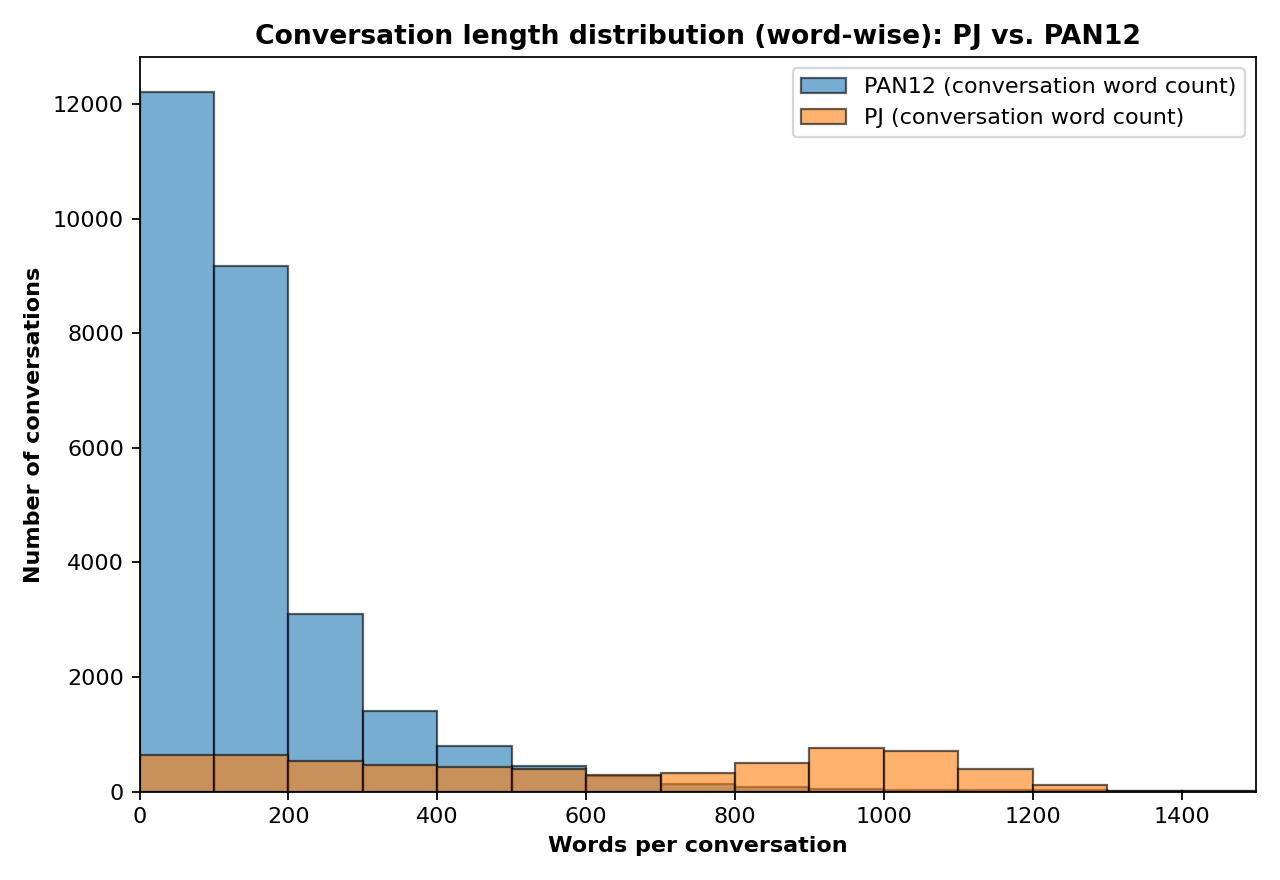
\includegraphics[width=0.75\textwidth]{conversation_word_lengths_pj_vs_pan12.png}
    \caption[Comparison of LIWC macro-groups]{Comparison of aggregated LIWC macro-groups between PAN12 (non-grooming) and PJ (grooming) over global conversations.}
    \label{fig:conversation_word_lengths}
\end{figure}

After initial preprocessing, the length distributions of the raw conversations in both datasets were analyzed. Figure~\ref{sec:chunk-length-distributions} shows the number of words per conversation for both PJ and PAN12 datasets. It is apparent, that PJ conversations are clearly longer than those from PAN12, with a \textbf{mean length of 609 words (PJ) versus 159 words (PAN12)}. This difference in length is a potential confounder, as the model could exploit it as a shortcut for classification instead of learning semantic patterns. Therefore, the preprocessing pipeline was designed to reduce this effect by enforcing fixed-length chunking and incorporating synthetic non-grooming data in PJ style.


\section{Generating Synthetic Non-Grooming Data}\label{sec:synthetic-data}

To further increase model robustness and mitigate dataset-specific artifacts, a custom script was developed that  uses the OpenAI API (\textit{gpt-4.1-mini}) to generate synthetic negative examples in the style of the Perverted Justice (PJ) data. The employed prompt contained the following rules:
\begin{enumerate}
\item \textbf{Replicate the linguistic style of PJ chats} by providing the model with 100 already normalized PJ conversations as few-shot examples.
\item \textbf{Enforce strict formatting}, requiring every line to follow the pattern \textit{speaker\_1: \textless text \textgreater} or \textit{speaker\_2: \textless text \textgreater}.
\item \textbf{Generate long dialogues} with 90–120 turns, in order to reduce the risk of length-based shortcuts. This choice was made because PJ conversations are usually much longer than those from PAN12 (see Figure \ref{fig:conversation_word_lengths} for a comparison of conversation length distributions).
\item \textbf{Restrict content} to everyday, harmless topics without any references to sexual activity.
\item \textbf{Include small imperfections} (e.g., occasional double dots, lowercase starts, or short fragments) to match the PJ normalization profile more closely, while keeping the conversations coherent.
\end{enumerate}

The synthetic data generation was done for the following two main purposes:

\begin{itemize}
    \item \textbf{Avoiding length leakage.} By generating long synthetic non-grooming conversations in PJ style, the data balance is improved and the reliance on length as a shortcut is reduced.
    \item \textbf{Avoiding domain leakage.} Since all PJ chats are labeled as class 0 and all PAN12 chats as class 1, the model could learn to separate classes only based on dataset-specific style differences. The synthetic PJ-style non-grooming data helps to reduce this effect by providing negative examples that mirror the PJ distribution without grooming semantics.
\end{itemize}

Unfortunately it was not possible to generate synthetic grooming conversations in the PAN12 style due to usage restrictions. Therefore, only non-grooming chats were created, ensuring that no artificial grooming data was introduced.


\section{Final Dataset}

The final dataset used for model training and evaluation consists of the following grooming and non-grooming conversations from the three sources: PJ, PAN12, and synthetic data. The final conversation counts are the following:

\begin{itemize}
    \item \textbf{PJ: 6175 Dialogues}
    \item \textbf{PAN12: 27755 Dialogues}
    \item \textbf{Synthetic: 600 Dialogues with mean lenght of 150 messages}
\end{itemize}


%%%geändert






\chapter{Methodology} \label{sec:methodology}
This chapter describes the methodology used in this work, including the BERT baseline model, the feature-fusion model architecture, the SHAP explainability analysis, and the analysis of misclassifications.
\section{Initial Chunking Strategy for BERT Fine-tuning}

The first preprocessing pipeline was developed to provide a straight BERT baseline for fine-tuning. Each conversation was reconstructed from the \textit{dialogue} field in the data into a single string with explicit speaker tags. Tokenization was then applied to the full conversation, with a maximum length of 512 tokens to provide the maximum information context in each chunk. Chunk boundaries could occur in the middle of a message. Conversations exceeding the 512 limit were split into non-overlapping chunks, which could occur at arbitrary positions within the text. Therefore, a single conversation could have multiple chunks, each treated as an independent training example. Finally, dynamic padding was applied at batch time and the tokenized dataset was then passed to the Hugging Face \textit{Trainer} for BERT fine-tuning without additional preprocessing steps.

%%%geändert 

\subsection{Train-Test Split}
For the finetuning, a train-test split was applied using \textit{GroupShuffleSplit} from \textit{sklearn}, ensuring, that all conversations from a single predator were contained completely in either the training or test set.  The split ratio was set to 70\% for training and 30\% for testing. Also, the same ratio of grooming to non-grooming conversations was kept in both sets to ensure balanced class distributions in the training and train and test data.

The resulting data distribution after chunking is shown in the following table.

\begin{table}[H] 
\label{tab:initial_split} 
\centering
\small
\caption[Initial data distribution after chunking]{\textbf{Initial data distribution after Chunking (max length 512, no message boundary control).}}
\begin{tabular}{lccc}
\hline
Split & Grooming & Non-Grooming PAN12  & \textbf{Total} \\
\hline
Train & 14997 & 30781  & \textbf{45778} \\
Test  & 1330 & 3429   & \textbf{4759} \\
\end{tabular}
\end{table}

%%%geändert

\section{BERT fine-tuning as Baseline}

Based on the initial chunking pipeline, BERT was fine-tuned for binary classification. 

The normal baseline followed a classic fine-tuning pipeline for binary classification with \textit{bert-base-uncased}. The training configuration was as follows:

\begin{itemize}
  \item \textbf{Backbone:} \textit{bert-base-uncased} (standard model dropouts)
  \item \textbf{Chunk length:} 512
  \item \textbf{Trainer/Optimization:} Hugging Face \textit{Trainer}
  \item \textbf{Epochs:} 3
  \item \textbf{Batch Size:} 8 
  \item \textbf{Learning Rate:} \textit{2e-5}
  \item \textbf{Weight Decay:} 0.01
  \item \textbf{Warmup:} none
  \item \textbf{Gradient Clipping:} not set
\end{itemize}



\subsection{Evaluation Metrics}
To evaluate the performance of the binary classifier, the most common metrics for a binary classification task were used in \textbf{all the following model evaluations}:

Let $TP$, $FP$, $TN$, and $FN$ be true positives, false positives, true negatives, and false negatives. 
The metrics are defined as follows:

\begin{align}
\text{Accuracy} &= \frac{TP + TN}{TP + TN + FP + FN}, \\
\text{Precision} &= \frac{TP}{TP + FP}, \\
\text{Recall} &= \frac{TP}{TP + FN}, \\
F_{1} &= 2 \cdot \frac{\text{Precision} \cdot \text{Recall}}{\text{Precision} + \text{Recall}}.
\end{align}

Therefore, Accuracy measures the proportion of correctly classified instances, while precision measures the proportion of predicted positive instances that are true positives. 
Recall measures the fraction of actual positive instances that are correctly identified, showing the model's ability to minimize false negatives. 
Finally, the $F_{1}$-score is reported as the harmonic mean of precision and recall, providing a balanced measure that accounts for both. 

Since the dataset is slightly imbalanced, the $F_{1}$-score for the positive class is used as the primary metric, ensuring that both precision and recall are equally considered for evaluation.

The evaluation was performed every 3000 steps during training, using the test dataset.

%%%geändert

\section{Limitations of Initial BERT Fine-tuning Approach}

\textbf{While the initial fine-tuning apporach enabled an effective baseline, it also included methodological concerns:}
\begin{enumerate}
  \item \textbf{Domain Leakage:} Since all PJ conversations have label 0 and all PAN12 conversations have label 1, the model could rely on dataset-specific artifacts (domain leakage) instead of semantic cues. As a result, the model might learn to distinguish between datasets rather than real grooming patterns.
  \item \textbf{Length Leakage:} In addition, PJ conversations are generally longer than the ones from PAN12 (Figure ~\ref{fig:conversation_word_lengths}), making conversation length a potential shortcut (length leakage). As a result, the model could exploit the length differences rather than learning real grooming-related features.
\end{enumerate}

\textbf{As shown later in the evaluation (Table ~\ref{tab:bert_base}), the initial model indeed achieved a very high performance, which motivated the design of a stricter preprocessing pipeline.} Therefore, a second preprocessing script was developed, which introduced fixed-length padding, enforced chunking at message boundaries, and included ynthetic non-grooming data in PJ style to reduce domain and length leakage. The following sections describe this improved pipeline in detail.

%% geändert
\section{Chunking Strategy for BERT to reduce Domain and Length Leakage}

To reduce leakage effects, a stricter preprocessing pipeline was implemented. Instead of splitting conversations at arbitrary positions, chunks were created only at message boundaries, ensuring that single utterances remained intact.

To further reduce domain leakage and length leakage, synthetic non-grooming chats in PJ style were added (Section~\ref{sec:synthetic-data}). Models were then trained and tested under the following two setups: 

\begin{enumerate}
  \item \textbf{Separated Split:} With synthetic data only in the test set, to probe generalization.
  \item \textbf{Mixed Split:} With synthetic data included in both train and test sets, to strengthen robustness.
\end{enumerate}


\subsection{Chunk-Length Distributions (For Train and Test) Across Sequence Lengths}\label{sec:chunk-length-distributions}

To determine the optimal chunk length for the BERT baseline, the mean, standard deviation, median, minimum, and maximum of tokens per conversation across the different datasets were calculated and are shown in table~\ref{tab:token_stats}. 

\begin{table}[htbp]
\centering
\caption{Token statistics per conversation/file across datasets}
\label{tab:token_stats}
\begin{tabular}{lrrrrrrr}
\toprule
\textbf{Dataset} & \textbf{Files} & \textbf{Mean} & \textbf{Std (pop)} & \textbf{Std (sample)} & \textbf{Median} & \textbf{Min} & \textbf{Max} \\
\midrule
PJ (grooming)                & 6\,175  & 723.83 & 446.54 & 446.58 & 719  & 12  & 1\,850 \\
PAN12                        & 27\,751 & 210.12 & 202.20 & 202.20 & 144  & 1   & 3\,656 \\
Synthetic                    & 621     & 969.47 & 161.24 & 161.37 & 972  & 488 & 1\,435 \\
PAN12 + Synthetic            & 28\,372 & 226.74 & 230.01 & 230.01 & 147  & 1   & 3\,656 \\
ALL (PJ + PAN12 + Synthetic) & 34\,547 & 315.59 & 339.65 & 339.65 & 171  & 1   & 3\,656 \\
\bottomrule
\end{tabular}
\end{table}

As again shown in table~\ref{tab:token_stats}, PJ conversations are much longer (mean: 724 tokens, median: 719 tokens) than PAN12 conversations (mean: 210 tokens, median: 144 tokens). The synthetic conversations are even longer (mean: 969 tokens, median: 972 tokens) and thus closer to the PJ distribution. The combined PAN12 + Synthetic dataset has a mean of 227 tokens and a median of 147 tokens, which is still much shorter than PJ. 
To evaluate the base model across these datasets, it was decided to test the baseline training with the following three fixed chunk sizes to evaluate, if the chunk size has an impact on performance and model robustness:
\begin{itemize}
  \item \textbf{150 tokens:} closely matches the PAN12 median while minimizing fragmentation for PAN12.
  \item \textbf{250 tokens:} offers additional context beyond the PAN12 median (covering a larger share of its distribution).
  \item \textbf{512 tokens:} contains full-length context for longer PJ/Synthetic conversations.
\end{itemize}

Consequently, the following three sequence lengths (150, 250, and 512) were generated, and padding on these fixed lengths was applied to test the impact of chunk size on performance, preventing the model from relying only on length differences between datasets.

%%%geändert

Figure~\ref{fig:chunk-dists} shows the resulting chunk length distributions for the three target lengths (150, 250, 512) after applying the improved chunking strategy, to show the impact of different chunk sizes on the dataset. Each subplot displays the distribution of chunk lengths in both training and test sets combined. The orange bars represent grooming chunks collected from PJ, while the blue bars represent non-grooming chunks collected from PAN12. Additionally the green bars show the synthetic non-grooming chunks in PJ style. The Chunk lengths were measured before padding on a fixed size of 512, 250 or 150 chunks was applied.


\begin{figure}[H]
  \centering
  \begin{subfigure}[t]{0.34\textwidth}\centering
    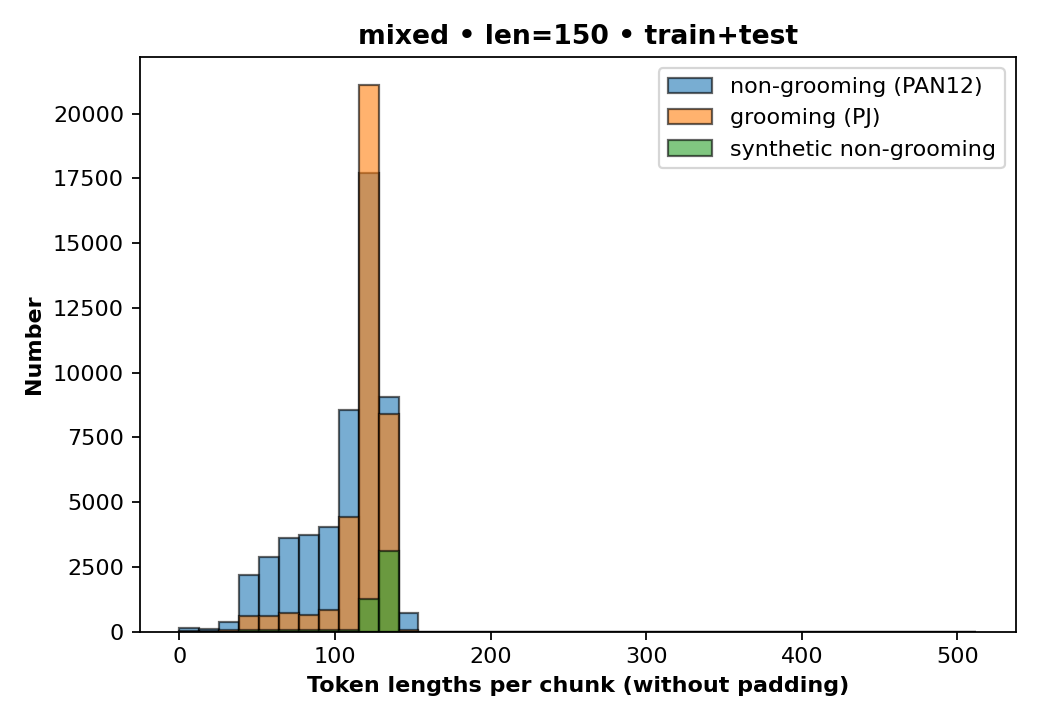
\includegraphics[width=\linewidth]{figures/chunkin_150_dist.png}
    \caption{150 tokens}\label{fig:chunkdist150}
  \end{subfigure}\hspace{-0.5em}% enger rücken
  \begin{subfigure}[t]{0.34\textwidth}\centering
    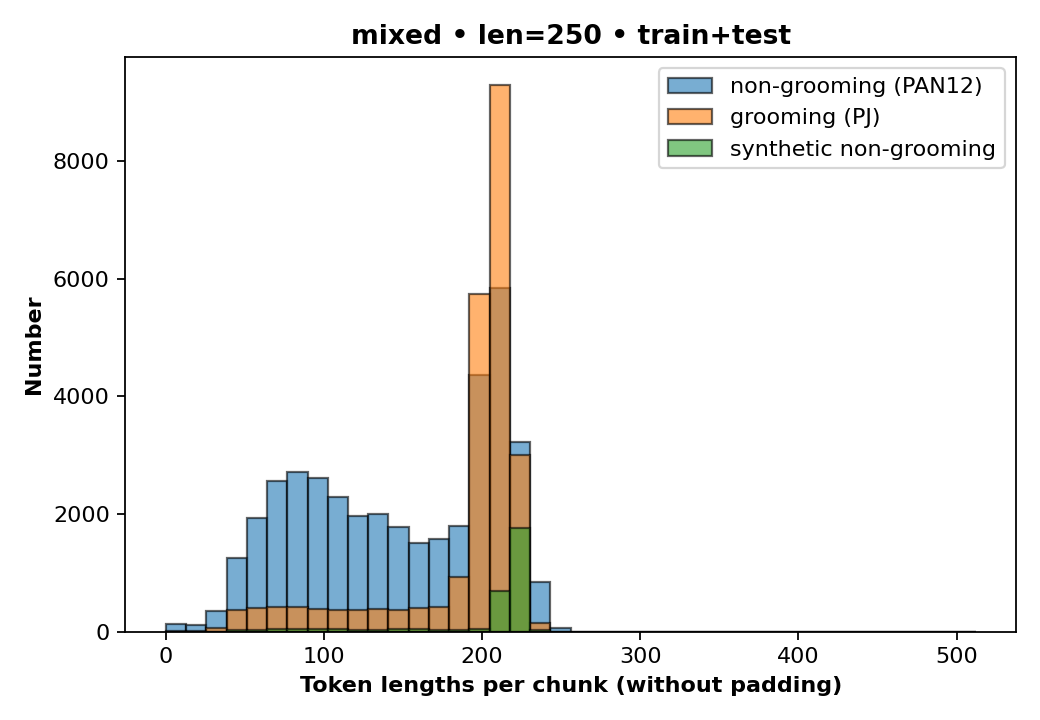
\includegraphics[width=\linewidth]{figures/chunking_250_dist.png}
    \caption{250 tokens}\label{fig:chunkdist250}
  \end{subfigure}\hspace{-0.5em}%
  \begin{subfigure}[t]{0.34\textwidth}\centering
    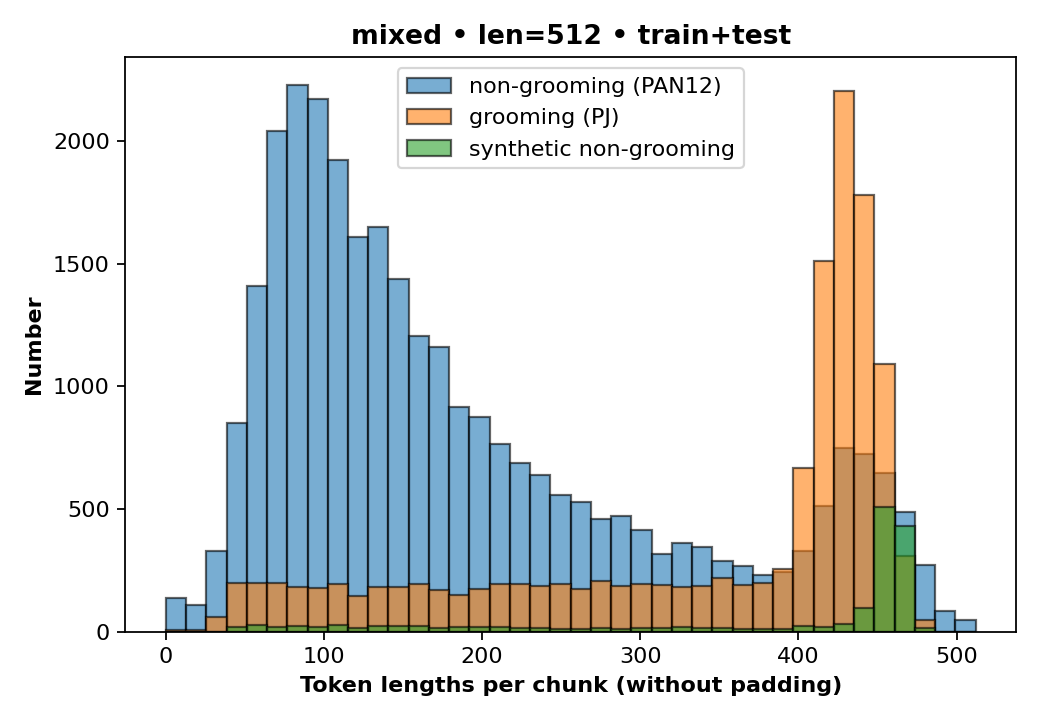
\includegraphics[width=\linewidth]{figures/chunking_512_dist.png}
    \caption{512 tokens}\label{fig:chunkdist512}
  \end{subfigure}
  \caption[Chunk Length Distributions]{Chunk length distributions (train+test) for different sequence lengths (before padding).}
  \label{fig:chunk-dists}
\end{figure}


\subsection{Data Distributions after Chunking}
 The following tables show the resulting data distributions after chunking for the three target lengths (150, 250, 512) and each setup (synthetic data only in test set and synthetic data in test and train set). Each table lists the number of chunks per class in the training and test sets for, together with the total number of chunks. 

 \begin{table}[H]
\centering
\small
\begin{tabular}{lcccc}
\hline
Split & Grooming & Non-Grooming PAN12 & Non-Grooming Synthetic & \textbf{Total} \\
\hline
Separated Train & 27883 & 36954 & 0    & \textbf{64837} \\
Separated Test  &  9625 & 16211 & 4749 & \textbf{30585} \\
\midrule[\heavyrulewidth]
Mixed Train     & 26583 & 37356 & 3254 & \textbf{67193} \\
Mixed Test      & 10925 & 15809 & 1495 & \textbf{28229} \\
\hline
\end{tabular}
\caption[Split for Chunk-Length of 150 Tokens]{\textbf{Split for Chunk-Length of 150 Tokens.}}
\end{table}


 \begin{table}[H]
\centering
\small
\begin{tabular}{lcccc}
\hline
Split & Grooming & Non-Grooming PAN12 & Non-Grooming Synthetic & \textbf{Total} \\
\hline
Separated Train & 17487 & 27057 & 0    & \textbf{44544} \\
Separated Test  &  6003 & 11848 & 2925 & \textbf{20776} \\
\midrule[\heavyrulewidth]
Mixed Train     & 16662 & 27321 & 2008 & \textbf{45991} \\
Mixed Test      &  6828 & 11584 & 917  & \textbf{19329} \\
\hline
\end{tabular}
\caption[Split for Chunk-Length of 250 Tokens]{\textbf{Split for Chunk-Length of 250 Tokens.}}
\end{table}


 \begin{table}[H]
\centering
\small
\begin{tabular}{lcccc}
\hline
Split & Grooming & Non-Grooming PAN12 & Non-Grooming Synthetic & \textbf{Total} \\
\hline
Separated Train & 9699 & 21259 & 0    & \textbf{30958} \\
Separated Test  & 3267 & 9195  & 1583 & \textbf{14045} \\
\midrule[\heavyrulewidth]
Mixed Train     & 9197 & 21352 & 1087 & \textbf{31636} \\
Mixed Test      & 3769 & 9102  & 496  & \textbf{13367} \\
\hline
\end{tabular}
\caption[Split for Chunk-Length of 512 Tokens]{\textbf{Split for Chunk-Length of 512 Tokens.}}
\end{table}



\section{Improved Training Pipeline} \label{sec:improved-training-pipeline}


For training on this improved dataset, the same BERT backbone was used but with a slightly more robust training configuration. Dropout rates in the classification head were increased (0.3), and label smoothing (0.1) was applied to reduce overconfidence. Gradient checkpointing was enabled for memory efficiency. 

\subsection{Improved Training Configuration}

The training configuration for the improved pipeline was the following:

\begin{itemize}
  \item \textbf{Backbone:} \textit{bert-base-uncased} with increased dropouts
  \item \textbf{Sequence length:} Variants \(\in \{150, 250, 512\}\) 
  \item \textbf{Dropout (BERT):} \(\textit{hidden\_dropout\_prob}=0.3\), \(\textit{attention\_probs\_dropout\_prob}=0.3\)
  \item \textbf{Loss function:} Cross-Entropy 
  \item \textbf{Label smoothing:} \(0.1\) 
  \item \textbf{Epochs:} \(3\)
  \item \textbf{Batch size:} \(8\)
  \item \textbf{Learning rate:} \(2\times10^{-5}\)
  \item \textbf{Weight Decay:} \(0.01\)
  \item \textbf{Warmup Ratio:} \(0.06\)
  \item \textbf{Max Grad Norm:} \(1.0\)
  \item \textbf{Gradient Checkpointing:} enabled 
\end{itemize}


\subsection{Evaluation Strategy with Additional Subsets}

The model was trained and tested across all three chunking target lengths (150, 250, 512) under two different setups
\begin{enumerate}
\item \textbf{Synthetic data only in the test set.}
This setup was designed to evaluate whether the model can generalize to PJ-style negatives without having seen them during training.
\item \textbf{Synthetic data in both train and test sets.}
This setup was designed to test whether including synthetic negatives in the training phase improves robustness and reduces reliance on dataset-specific artifacts.
\end{enumerate}

The evaluation was again performed every 3000 steps on the test set, using accuracy, precision, recall, and F1 score as metrics. 

To further test robustness, an evaluation callback ran three subsets after each evaluation step:
\begin{itemize}
\item \textbf{Real-only test set (consisting of only PAN12 + PJ data).}
\item \textbf{Synthetic-only test set.}: Here the model was only evaluated based on the accuracy since precision, recall, and F1 are not defined for a single class.
\end{itemize}

Additionally the confusion matrix was calculated for the complete test set after each evaluation step to analyze the types of errors made by the model. Also, the ROC-Curve and the AUC score were calculated after each evaluation step to analyze the model's performance across different classification thresholds.

The detailed outcomes the training across alle different chunk size and train/test split configurations are shown in the evaluation section (Section~\ref{sec:bert_chunk_size_and_data_setup}).

\section{Choosing the final configuration for Feature Fusion and SHAP Explainability Analysis} 

%%Überarbeitet

Based on the evaluation across different chunk sizes and dataset configurations (Section \ref{sec:bert_chunk_size_and_data_setup}), \textbf{it was decided to continue the feature fusion and explainability analysis with a chunk size of 512 tokens in combination with the mixed split strategy}. Although shorter chunks were hypothesized to reduce length leakage, the results show no significant performance improvement for 150 or 250 tokens. Instead, 512-token chunks consistently achieved the best F1 scores (up to 0.97) while at the same time providing richer conversational context, which is crucial for a clean LIWC analysis. Moreover, the separated split revealed poor generalization, indicating overfitting on training data. By contrast, the mixed split setup led to more robust performance across evaluation subsets, making it the more reliable and realistic configuration for further experiments. Therefore, this final choice balances model accuracy with interpretability and robustness, setting a solid foundation for the following feature fusion experiments and shap analyses.


\section{Choosing the LIWC Feature Set for Feature Fusion and SHAP Explainability Analysis} \label{sec:liwc-feature-selection}

%% überarbeitet


\textbf{The Feature-Fusion and following SHAP explainability analysis was performed with two variants of feature sets in each case: }
\begin{enumerate}
    \item \textbf{All-Features-Fusion}: Use of all 118 LIWC features.
    \item \textbf{Psychometric-Fusion}: Use of a subset of \textbf{49 psychometric LIWC features} coverings all psycholinguistic LIWC features that are highlighted in the literature as relevant for manipulative communication in Grooming Chats (Section \ref{psychometric_liwc_features_in_grooming}). The subset contains the following categories and dimensions:
\end{enumerate}

\paragraph{Psychometric LIWC Subset (49 features).}
\begin{itemize}
  \item \textbf{Drives}: \textit{Drives}, \textit{affiliation}, \textit{achieve}, \textit{power}, \textit{reward}, \textit{risk}, \textit{curiosity}, \textit{allure}
  \item \textbf{Cognition}: \textit{Cognition}, \textit{allnone}, \textit{cogproc}, \textit{insight}, \textit{cause}, \textit{discrep}, \textit{tentat}, \textit{certitude}, \textit{differ}, \textit{memory}
  \item \textbf{Affect \& Emotion}: \textit{Affect}, \textit{tone\_pos}, \textit{tone\_neg}, \textit{emotion}, \textit{emo\_pos}, \textit{emo\_neg}, \textit{emo\_anx}, \textit{emo\_anger}, \textit{emo\_sad}, \textit{swear}
  \item \textbf{Social}: \textit{Social}, \textit{socbehav}, \textit{prosocial}, \textit{polite}, \textit{conflict}, \textit{moral}, \textit{comm}, \textit{socrefs}, \textit{family}, \textit{friend}, \textit{female}, \textit{male}
  \item \textbf{Physical/Biological}: \textit{Physical}, \textit{health}, \textit{illness}, \textit{wellness}, \textit{mental}, \textit{substances}, \textit{sexual}, \textit{food}, \textit{death}
\end{itemize}
\textbf{The idea for this two-staged approach was to evaluate whether a set of only psycholinguistically relevant features could provide similar or better interpretability and performance compared to using the full LIWC-2022 feature set.} 


\section{LIWC Data Extraction}

The LIWC features were extracted using the official LIWC-22 software. The extraction was done once over complete PJ and PAN12 conversations as well as the synthetic non-grooming conversations in PJ style. Furthermore, the LIWC features were also extracted for each chunk in the improved chunked dataset with a chunk size of 512 tokens(Section \ref{sec:methodology}).

Also, the LIWC Features were extracted in two variants: once with all 118 features and once with the psychometric subset of 49 features (Section \ref{sec:liwc-feature-selection}). The extracted LIWC features were then stored in a separate sidecar file.

\section{LIWC Data Analysis}

In order to analyze the effect size of LIWC features prior to fine-tuning, a comprehensive analysis of LIWC features across all conversations was performed.
The LIWC-based analysis was carried out in two steps. First, a global comparison was performed on complete conversations, followed by a chunk-based comparison using 512 chunks, which was tailored to the subsequent feature fusion. Both analyses were performed once for the complete set of LIWC-2022 features and once restricted to the psychometric subset of LIWC features to determine whether psychometric variables alone are sufficient to distinguish grooming conversations from non-grooming conversations.

\subsection{Global LIWC Analysis on Complete Conversations}

For the global analysis, all grooming conversations from the PJ were first aggregated into one conversation per groomer to represent their general language style, while non-grooming conversations from PAN12 were used in their original form. 
For each conversation, the complete set of LIWC-2022 features was calculated.  
To improve interpretability, the features were grouped into macro categories according to the LIWC-2022 manual:

\begin{itemize}
    \item \textbf{Linguistic:} Function, pronoun, ppron, i, we, you, shehe, they, ipron, det, article, numeral, preposition, auxiliary verb, adverb, conjunction, negation, verb, adjective, quantity
    \item \textbf{Punctuation:} Period, comma, question mark, exclamation mark, apostrophe, other
    \item \textbf{Emoji:} Emoji
    \item \textbf{Drives:} Belonging, Achievement, Power
    \item \textbf{Motivation:} Reward, Risk, Curiosity, Enticement
    \item \textbf{Cognition:} Cognition, allnone, cogproc, Insight, Cause, Discrepancy, Attempt, Certainty, Difference, Memory
    \item \textbf{Affect:} Positive tone of voice, negative tone of voice, emotion, positive emotion, negative emotion, fear, anger, sadness, swearing
    \item \textbf{Social:} Social behavior, prosocial, polite, conflict, morality, communication, social references, family, friend, female, male, social
    \item \textbf{Physical:} Health, illness, well-being, mental, substances, sexual, food, death, physical
    \item \textbf{Perception:} Attention, movement, space, visual, auditory, feeling
    \item \textbf{Culture:} Politics, ethnicity, technology
    \item \textbf{States:} Need, desire, acquisition, lack, fulfillment, fatigue
    \item \textbf{Time:} Time, focus on the past, focus on the present, focus on the future
    \item \textbf{Conversation:} Internet slang, agreement, non-fluency, filler words
\end{itemize}

For each conversation, the value of a macro group was defined as the arithmetic mean of all available member characteristics. Subsequently, the macro group means were averaged across all conversations for each class (PJ vs. PAN12). 
The results were visualized as grouped bar charts (PJ vs. PAN12) sorted by the overall mean \(\tfrac{1}{2}(\overline{g}_{\mathrm{PJ}}+\overline{g}_{\mathrm{PAN}})\) .

In addition to macro group aggregation, each individual LIWC feature was statistically analyzed. For each feature \(f\), the mean and standard deviation across all conversations were calculated per class,
\[
\overline{x}_{\mathrm{PJ}},\ s_{\mathrm{PJ}},
\qquad
\overline{x}_{\mathrm{PAN}},\ s_{\mathrm{PAN}},
\]
followed by the mean difference \(\Delta = \overline{x}_{\mathrm{PJ}} - \overline{x}_{\mathrm{PAN}}\) and Cohen's \(d\) \cite{cohen1988},
\[
d = \frac{\Delta}{s_p},
\qquad
s_p = \sqrt{\frac{(n_{\mathrm{PJ}}-1)s_{\mathrm{PJ}}^2+(n_{\mathrm{PAN}}-1)s_{\mathrm{PAN}}^2}{n_{\mathrm{PJ}}+n_{\mathrm{PAN}}-2}}.
\]


The descriptive statistics and effect sizes were compiled into a summary table for all LIWC features which is provided in the appendix (table \ref{tab:liwc22-categories}).

Furthermore, the 30 LIWC-2022 features with the largest absolute effect sizes \(|d|\) were selected to identify the most discriminative variables. 
This procedure was performed twice. Once for the complete set of LIWC features and once restricted to the psychometric LIWC subset to analyze if psychometric features alone capture the major differences between the two classes. 

To further assess the quality and representativeness of the synthetically generated non-grooming data, an additional global LIWC analysis was conducted comparing PJ Grooming and PAN12 Non-Grooming to the synthetic dataset. 
For each comparison, Cohen’s \(d\) was again computed for all LIWC features, and the top 30 features by absolute effect size were visualized as horizontal bar plots. 
This step was intended to identify potential linguistic deviations between the synthetic and real-world data and to evaluate whether the synthetic data exhibits similar psycholinguistic patterns as PAN12.

The results of the global LIWC analysis are presented in the evaluation section (Section~\ref{sec:global_liwc_analysis}).

\subsection{Chunk-based LIWC Analysis with 512 Tokens}

To examine patterns within conversations, a chunk-based analysis was performed with a fixed chunk size of 512 tokens (identical to the size later used for model training). For each chunk, a LIWC-2022 feature vector was calculated and the average values per class were determined across all chunks. also based on the data level , which
For each feature, the range
\[
\mathrm{range}(f) = \max_{s}\overline{f}_{s} - \min_{s}\overline{f}_ {s}
\]
was determined for each feature across all sources (\(s \in \{\mathrm{PJ}, \mathrm{PAN12}, \mathrm{SYN}\}\)), and the \(K=15\) features with the largest ranges were selected for visualization.
Two heatmaps were created: one limited to these 15 most important distinguishing features and one containing all available features (in alphabetical order).The rows represent PJ Grooming, Synthetic Non-Grooming, and PAN12 Non-Grooming, while the columns represent the LIWC features.
This process was repeated once for all LIWC features and once for the psychometric features to determine whether psychometric variables alone exhibit comparable distinction at the chunk level.

The visualization and evaluation of the chunk-based LIWC analysis is presented in section~\ref{sec:chunk_based_liwc_analysis}.

\section{Feature Fusion Strategy}

%%Überarbeiter

To extend the BERT baseline with the additional input of LIWC features, the LIWC features were first extracted for all chunks from the dataset with 512 tokens and stored as numerical vectors in a separate sidecar file.  For this purpose, the sidecar contained a key consisting of \textit{conv\_id} and \textit{chunk\_index} for each chunk, as well as the corresponding chunk-specific LIWC features. 
When loading the dataset, these sidecar files were assigned to the respective chunks based on the \textit{conv\_id} and the \textit{chunk\_index} (for dialogues consisting of several chunks), so that the training and test data sets then contained an additional column for \textit{liwc} in addition to \textit{input\_ids}, \textit{attention\_mask}, and \textit{labels}. \newline

To integrate the LIWC features into the BERT architecture, \textbf{a late fusion approach} was implemented using cross-attention and a gating mechanism. This method allowed the model to select information from LIWC into the contextualized token representations learned by BERT. 

\subsection{Model Architecture}

The proposed feature fusion model extends \textit{bert-base-uncased} (12 transformer layers, hidden size \(d_h=768\), 12 attention heads) with a late-fusion mechanism that integrates psycholinguistic LIWC features into the transformer encoder in the upper encoder layers at layer 6 and 12. The design was used to keep the original BERT architecture and its pre-trained weights intact while allowing the model to leverage additional psycholinguistic information from LIWC. This keeps the tokenization and main contextual processing of the text unchanged, while the LIWC information is only introduced after language modeling, which holds comparability with the BERT baseline and allows a later downstream explainability using SHAP. The overall process can be summarized as followed:

\begin{itemize}
    \item \textbf{Input and Feature Projection:}
    \begin{itemize}
        \item For each text chunk, a LIWC feature vector \(x \in \mathbb{R}^{d_{liwc}}\) is extracted 
        (\(d_{liwc}=118\) for all features or \(d_{liwc}=49\) for the psychometric subset).
        \item \(x\) is normalized using \textit{LayerNorm} and mapped through a linear projection with \textit{GELU} activation to a compact fusion dimension \(z \in \mathbb{R}^{d_p}\) (\textit{proj\_dim}, e.g., 128/768).
        \item From \(z\), a single \emph{LIWC token} \(t \in \mathbb{R}^{d_h}\) is generated via a linear layer. 
        This token summarizes the psychometric information for the entire chunk.
    \end{itemize}

    
    \item \textbf{Fusion via Cross-Attention:}
    \begin{itemize}
        \item Text hidden states \(H \in \mathbb{R}^{T \times d_h}\) from intermediate layers serve as \textbf{queries}.
        \item The LIWC token \(t\) is used as \textbf{key/value} in a multi-head cross-attention mechanism (\textit{n\_heads}=4, mask-aware).
        \item This enables each token to attend to the psycholinguistic context selectively.
    \end{itemize}
    
    \item \textbf{Gating and Residual Update:}
    \begin{itemize}
        \item A channel-wise gate \(g \in \mathbb{R}^{d_h}\) (\textit{gate\_type}=\textit{channel}) is computed from the \textit{[CLS]} representation and \(z\).
        \item The final representation is updated via
        \[
        H' = H + g \odot \mathrm{Attn}(H, t)
        \]
        followed by a 10\% dropout.
        \item A post-fusion \textit{LayerNorm} is applied to stabilize training and normalize the residual update.

    \end{itemize}
    
    \item \textbf{Integration in Encoder:}
    \begin{itemize}
        \item The fusion block is applied in the upper encoder layers (layers 6 and 12; \textit{fusion\_at\_layers} with \textit{depth}=1).
        \item After the final fusion layer, the \textit{[CLS]} vector is pooled as in the baseline model and passed to a linear classification head.
        \item  The pooled \textit{[CLS]} representations are combined either by averaging (\textit{mean}). The resulting fused representation is then passed to the linear classifier.

    \end{itemize}
\end{itemize}
    
    

The overall feature-fusion architecture is illustrated in the following figure~\ref{fig:liwc-bert-fusion}.

\begin{figure}[H]
    \centering
    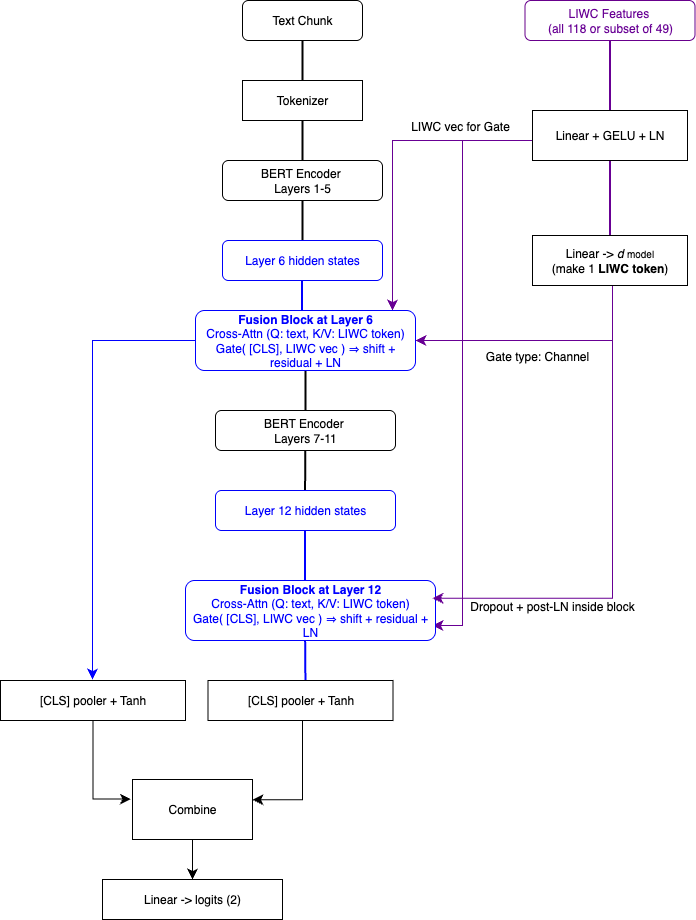
\includegraphics[width=0.7\textwidth]{new_fusion.png}
    \caption[Feature Fusion Architecture]{Late fusion of LIWC with BERT: LIWC features (either all 118 or the 49 psychometric subset) are projected, transformed into a single \emph{LIWC token}, and fused with hidden states from layers 6 and 12 via cross-attention plus a gating mechanism (Multimodal Shifting). The resulting fusion blocks are applied in parallel to the BERT encoder and do not feed back into subsequent layers. The [CLS] representations from both fusion points are pooled, combined, and classified. The \textcolor{blue!70!black}{blue blocks} highlight where fusion takes place, while the \textcolor{violet!70!black}{purple line} represents the LIWC stream (projection and token).}
\label{fig:liwc-bert-fusion}

\end{figure}

\subsection{Training Pipeline and Evaluation}

The training and evaluation of the feature fusion model followed a similar pipeline as the improved BERT-Baseline (Section~\ref{sec:improved-training-pipeline}). With the following hyperparameters:

\begin{itemize}
\item \textbf{Number of Epochs:} \(3\) 
\item \textbf{Saving Checkpoint at Epoch:}\(1\) 
\item \textbf{Evaluation Steps:} \(3000\)
\item \textbf{Learning Rate:} \(2\times10^{-5}\)
\item \textbf{Weight Decay:} \(0.01\)
\item \textbf{Warmup Ratio:} \(0.06\)
\item \textbf{Max Grad Norm:} \(1.0\)
\item \textbf{Batch Size:} \(8\)
\item \textbf{Loss Function:} Cross-Entropy with Label Smoothing of \(0.1\)
\item \textbf{Dropout inside Fusion} \(0.1\)
\item \textbf{Number of Heads in Cross-Attention:} \(4\)
\item \textbf{Fusion Depth:} \(1\)
\end{itemize}

The Evaluation was performed with the same metrics as in the BERT-Baseline (accuracy, precision, recall, F1) and on the dataset with chunks consisting of 512 tokens and synthetic data in both train and test set. The evaluation was done every 3000 steps of training and the model was stored after each epoch.




\section{Explainability Analysis based on Feature Fusion Model}

The following Analysis was done based on the Feature Fusion Model with a Chunk size of 512 tokens and Synthetic Data in both Train and Test set after \textbf{three epochs of training}. This decision was made to ensure that the model had sufficient exposure to the data and to capture more complex patterns in the feature interactions.

To analyze the model's decision-making process, SHAP was used to show insights into how both token-level text features and LIWC psychometric features contributed to the model's predictions. The following sections describe the two complementary explainability analyses that were conducted.


\subsection{SHAP analysis of LIWC features} \label{sec:shap_analysis_of_liwc_features}

To understand which psycholinguistic features are relevant for the classification decision, a SHAP analysis of the LIWC features was performed. Both the complete LIWC feature set with 118 dimensions and a psychometric subset with 49 selected categories were considered. The fixed-length LIWC vector calculated for each chunk served as input for the analysis. 

\subsubsection{Reducing Computational Costs with KernelSHAP}
The explanations were generated using KernelSHAP, whereby the text input of the model was capped to a fixed sequence length and kept constant for all explanations. To keep the computational costs of the SHAP analysis manageable, a fixed configuration was used for both the complete LIWC feature set (118 dimensions) and the reduced psychometric subset (49 dimensions).  \texttt{3000} random samples from the test set were selected for explanation. To mitigate class-imbalance bias, all global statistics are computed on a \textbf{class-balanced subset} of the test set (50\% grooming, 50\% non-grooming). For the background distribution, \texttt{32} LIWC vectors were chosen and reduced to at most 20 representative centroids using k-means clustering. Each instance was then perturbed \texttt{256} times in order to approximate the marginal feature contributions. 

The model was executed in mini-batches of \textit{4} explanations, with a maximum of \textit{16} perturbations processed in parallel. In addition, the text input was capped to a constant sequence length of \texttt{64} tokens, and inference was carried out in mixed precision with disabled gradients. These measures reduced GPU memory consumption and made it feasible to perform KernelSHAP for both feature sets without exceeding hardware limits.

\subsubsection{Determining Feature Importance and Direction of Effect}

The model’s \emph{grooming} (positive) logit was explained using KernelSHAP while the \textbf{text representation was held fixed} and only the LIWC feature vector was perturbed.

\paragraph{Global importance.}
For each LIWC feature $i$, the contribution over the balanced subset was aggregated via the \textbf{mean absolute} SHAP value, $\mathrm{mean}|\mathrm{SHAP}|_i$, and reported as normalized percentages for readability:
\[
\text{FeatureImportance}_{i}
= \frac{\mathrm{mean}\,|\mathrm{SHAP}|_{i}}{\sum_{j=1}^{F} \mathrm{mean}\,|\mathrm{SHAP}|_{j}} \times 100\% ,
\]
where $F$ is the number of LIWC features. This quantifies the share of the model’s decision attributable to feature $i$.

Based on the global Importance, the commulative importance of every LIWC features were determined by sorting the features descendingly and calculating the cumulative sum of the importance values. 

\paragraph{Direction of effect.}
\textbf{Signed} SHAP values according to the grooming logit indicate direction:
\[
\mathrm{SHAP}^{(+)}_{i} > 0 \;\Rightarrow\; \text{feature } i \text{ pushes the prediction toward grooming,}
\]
\[
\mathrm{SHAP}^{(+)}_{i} < 0 \;\Rightarrow\; \text{feature } i \text{ pushes the prediction toward non-grooming.}
\]

\subsubsection{Partitioning overall contribution into tokens vs.\ LIWC}\label{sec:token_vs_liwc_share}

To quantify the relative contribution of text tokens versus LIWC features to the model's decisions, two complementary attribution procedures were computed on the same set of explained instances and subsequently paired.

\paragraph{Token-side attribution (Integrated Gradients).}
For each instance, token-level attributions were obtained with Integrated Gradients on the embedding input.
A zero embedding served as baseline, and attributions were computed with regard to the model's predicted class.
Let $a_{n,t}\in\mathbb{R}^d$ denote the IG vector for token $t$ in instance $n$ (embedding dimension $d$).
A scalar saliency per token was formed via the $\ell_2$ norm and aggregated across tokens to give a per-instance token total:
\[
S^{\mathrm{tok}}_{n}
\;=\;
\sum_{t} \lVert a_{n,t}\rVert_2.
\]
During IG, the LIWC branch was held fixed to a constant vector (median over the sidecar features) to avoid confounding text and LIWC effects.

\paragraph{LIWC-side attribution (KernelSHAP).}
For the same instances, LIWC attributions was again computed with KernelSHAP by varying the LIWC feature vector while keeping the text input fixed to a short sequence.
Let $\phi_{n,f}$ denote the SHAP value of LIWC feature $f$ for instance $n$.
Per-instance LIWC totals were formed by summing absolute SHAP values across features:
\[
S^{\mathrm{liwc}}_{n}
\;=\;
\sum_{f=1}^{F} \lvert \phi_{n,f}\rvert .
\]

Because the classifier has two output classes, KernelSHAP returns one attribution per class. Therefore class-agnostic attributions were used by averaging the absolute SHAP values across classes for each instance and feature before aggregation.

\paragraph{Pairing and normalization.}
For each explained instance \(n\), the two totals were combined into percentage shares:
\[
\mathrm{Share}^{\mathrm{liwc}}_{n}
\;=\;
\frac{S^{\mathrm{liwc}}_{n}}{S^{\mathrm{liwc}}_{n}+S^{\mathrm{tok}}_{n}}
\;\times\;100\%,
\qquad
\mathrm{Share}^{\mathrm{tok}}_{n}
\;=\;
\frac{S^{\mathrm{tok}}_{n}}{S^{\mathrm{liwc}}_{n}+S^{\mathrm{tok}}_{n}}
\;\times\;100\% .
\]
Global summaries were reported as the mean and median of these per-instance percentages over \(N=1000\) randomly sampled test instances.


\subsection{Confidence Analysis based on Label Flip and Confidence Shift}

To further analyze the impact of LIWC features on model decisions, model confidence and class assignment were calculated once with the regular LIWC feature vectors (\emph{LIWC on}) and once with LIWC vectors set to zero (\emph{LIWC off}). This allowed the influence of the additional LIWC features on model confidence and class assignment to be analyzed.

For both conditions, the class probability was determined by applying the softmax function to the logits. The highest probability \(p_{\max}\) represents the model confidence for the predicted class:
\[
p_{\max}^{(\text{on})} = \max_k p_k^{(\text{LIWC on})}, \qquad
p_{\max}^{(\text{off})} = \max_k p_k^{(\text{LIWC off})}.
\]

The difference between these two values defines the so-called \textbf{confidence shift}:
\[
\Delta p_{\max} = p_{\max}^{(\text{on})} - p_{\max}^{(\text{off})}.
\]
A positive value indicates that the LIWC features increased the certainty of the model decision, while a negative value describes a decrease in confidence.

In addition, it was analyzed whether the predicted class of an input changed as a result of LIWC fusion (for example, model decision = grooming before and model decision = non-grooming after). If such a change occurs, it is referred to as a \textbf{label flip}:
\[
\text{flip} = \mathbb{1}\!\left[\,\hat{y}^{(\text{on})} \neq \hat{y}^{(\text{off})}\,\right], 
\qquad
\hat{y} = \arg\max_k p_k.
\]
The number and rate of label flips show the extent to which the LIWC features lead to a changed classification decision.

For quantitative analysis, the following metrics were calculated:
\begin{itemize}
    \item $\Delta \mu$, $\Delta \tilde{x}$, $\Delta \sigma$: Mean, median, and standard deviation of \(\Delta p_{\max}\).
    \item $\Delta p_{10}$, $\Delta p_{90}$: 10th and 90th percentiles of the distribution of \(\Delta p_{\max}\).
    \item $n_{\text{class 0}}$, $n_{\text{class 1}}$: Frequency distribution of the predicted classes with LIWC.
    \item $n_{\text{flips}}$, flip rate: Number and relative frequency of prediction changes.
\end{itemize}


The results are presented in Section ~\ref{sec:confidence_and_label_flip_analysis}.

\section{LIWC Analysis of Misclassifications}

To identify potential patterns in the misclassifications made by the feature fusion model, a LIWC analysis of false positives and false negatives was conducted. It was tested whether misclassified samples resemble the opposite correct class in LIWC space, i.e., whether false negatives are closer to true negatives and false positives are closer to true positives according to their LIWC Feature values. Furthermore, it was analyzed which LIWC features differ significantly between misclassified and correctly classified samples. This analysis was again conducted with both the full LIWC feature set and the psychometric subset. The same fusion model, tokenizer, and LIWC sidecar vectors as in the previous sections were used to generate predictions and per-sample LIWC vectors. The analysis was performed on the complete test set.

\subsection{Per-feature group comparisons}
Per-feature comparisons were run for four group pairs: FP vs.\ TN, FN vs.\ TP, TN vs.\ FN, and TP vs.\ FP. For each LIWC feature \(f\), let \(x\) denote values in the first named group and \(y\) in the second. The following statistics were computed:

\begin{itemize}
\item \textbf{Mean difference} \(\Delta\mu = \bar{x} - \bar{y}\).
\item \textbf{Again, Cohen's \(d\)  was used to quantify effect size}
\item \textbf{Significance tests.} The Mann–Whitney \(U\) test (two-sided) was used to assess the significance of differences in distributions of FP/TN and FN/TP.
\item \textbf{Multiple testing control.} The Benjamini–Hochberg procedure was applied across features to obtain FDR-adjusted \(q\)-values. For plotting, a significance score \(-\log_{10}(q)\) was used.
\end{itemize}


\subsection{Proximity hypothesis tests in LIWC feature space}
To test whether misclassifications resemble the opposite correct group in LIWC space, distances were computed in standardized feature space (z-scored per LIWC dimension). Let \(\mathbf{c}_{\mathrm{TN}}\) and \(\mathbf{c}_{\mathrm{TP}}\) be the centroids of TN and TP, respectively. For each FN sample with standardized vector \(\mathbf{z}\), Euclidean distances
\(d_{\mathrm{TN}} = \|\mathbf{z}-\mathbf{c}_{\mathrm{TN}}\|_2\) and
\(d_{\mathrm{TP}} = \|\mathbf{z}-\mathbf{c}_{\mathrm{TP}}\|_2\) were computed and the following one-sided hypotheses were tested:
\[
H_{1}^{\mathrm{FN}}:\; \Pr\!\big[d_{\mathrm{TN}} < d_{\mathrm{TP}}\big] > 0.5
\quad\text{and}\quad
H_{1}^{\mathrm{FP}}:\; \Pr\!\big[d_{\mathrm{TP}} < d_{\mathrm{TN}}\big] > 0.5.
\]
For each hypothesis, the analysis reports:

\begin{itemize}
  \item \textbf{Proportion of samples} closer to the hypothesized centroid:
  \[\hat{p} = \frac{1}{n}\sum_{i=1}^{n} \mathbb{1}[d_{\text{closer}} < d_{\text{farther}}].\]
  \item \textbf{One-sided binomial test} against \(0.5\) to assess whether the observed proportion \(\hat{p}\) is significantly greater than chance.
  \item \textbf{Paired one-sided tests} on the distance differences \(d_{\mathrm{TN}} - d_{\mathrm{TP}}\) for FN and \(d_{\mathrm{TP}} - d_{\mathrm{TN}}\) for FP. Both the Wilcoxon signed-rank test and the one-sample \(t\)-test were used to assess whether the mean/median difference is significantly greater than zero.
\end{itemize}

The results of the LIWC analysis of misclassifications are presented in section \ref{sec:misclassification_analysis}.

\subsection{SHAP-Based Proximity Analysis of Top-20 Misclassifications}


For a deeper analysis of misclassifications, an evaluation was performed based on the \textbf{top 20 LIWC features}, which were identified in Section~\ref{sec:shap_analysis_of_liwc_features} as the most relevant using global SHAP values (\emph{mean\_abs}) and explain the majority of model decisions. This allows examining whether misclassifications can be explained by their proximity to the opposite correct class along these LIWC dimensions. Also, focusing on the 20 most important features reduces noise from less informative variables and enables a more targeted analysis of group differences.

\paragraph{Top-20 selection and SHAP direction.}
All LIWC-2022 features were globally ranked by their \emph{mean\_abs} SHAP values, and the top 20 were selected. In addition, the SHAP sign (\emph{mean\_signed}) was used for each feature to define the “TP-like” versus “TN-like” direction.

All LIWC-2022 features were globally ranked by their \emph{mean\_abs} SHAP values on a class-balanced subset (50\% grooming, 50\% non-grooming), and the top 20 were selected. For each feature, the SHAP sign (\emph{mean\_signed}) with respect to the grooming logit was used to define the “TP-like” versus “TN-like” direction.

\paragraph{Z-scaling and SHAP-oriented projection.}
To ensure comparability, feature columns were $z$-scaled. Each feature was then \emph{projected} onto the SHAP direction by multiplying, per sample, with the sign of its \emph{per-class SHAP margin}, i.e.\ $\operatorname{sign}(\Delta\mathrm{SHAP}_i)$ with
$\Delta\mathrm{SHAP}_i = \mathrm{SHAP}^{(+)}_i - \mathrm{SHAP}^{(-)}_i$ (grooming = $+$, non-grooming = $-$; default class indices 1 and 0). On this aligned axis, values to the right of $x=0$ indicate greater similarity to true positives (TP-like), and values to the left indicate greater similarity to true negatives (TN-like). In both cases, multiplying $z$-scaled feature values by this sign yields a SHAP-aligned axis where values $>0$ are TP-like and values $<0$ are TN-like.


\paragraph{Group statistics and confidence intervals.}
For each group $\{\mathrm{TP}, \mathrm{TN}, \mathrm{FP}, \mathrm{FN}\}$ and each top-$K$ feature, group means $\bar{x}$, standard deviations $s$, and standard errors
\[
SE \;=\; \frac{s}{\sqrt{n}}
\]
with $n$ as the group size were calculated on the projected values. For the misclassification groups (FP and FN), a 95\% confidence interval was computed as
\[
\mathrm{CI}_{95} \;=\; \bar{x} \pm 1.96 \cdot SE.
\]
The position of this interval relative to $x=0$ was classified as:
\emph{TP-side} (entirely $>0$), \emph{TN-side} (entirely $<0$), \emph{crosses-0} (ambiguous), or \emph{unknown} (no SE/CI available).

\paragraph{Proximity rate (TP/TN closeness).}
To assess whether misclassifications align more with TP or TN, per feature the absolute distances on the projected axis were compared:
\[
d_{\mathrm{FP}\to\mathrm{TP}} \;=\; \bigl|\bar{x}_{\mathrm{FP}} - \bar{x}_{\mathrm{TP}}\bigr|,\quad
d_{\mathrm{FP}\to\mathrm{TN}} \;=\; \bigl|\bar{x}_{\mathrm{FP}} - \bar{x}_{\mathrm{TN}}\bigr|,
\]
and analogously for FN. A feature is counted as “FP closer to TP” if $d_{\mathrm{FP}\to\mathrm{TP}} < d_{\mathrm{FP}\to\mathrm{TN}}$, and as “FN closer to TN” if $d_{\mathrm{FN}\to\mathrm{TN}} < d_{\mathrm{FN}\to\mathrm{TP}}$. Summary rates are reported over the top-20 features. 

\paragraph{Summary measures.}
The following aggregated values were derived:
\begin{itemize}
  \item \textbf{Proximity rate}: proportion of features supporting the expected proximity (FP\(\rightarrow\)TP or FN\(\rightarrow\)TN),
  \item \textbf{CI TP-side (n)}: number of features with 95\% CI fully to the right of 0,
  \item \textbf{CI TN-side (n)}: number of features with 95\% CI fully to the left of 0,
  \item \textbf{CI crosses 0 (n)}: number of features with 95\% CI intersecting 0 (ambiguous).
\end{itemize}

The results of this analysis, including visualization and summary tables, are presented in Section~\ref{sec:shap_missclassification_analysis}.



\chapter{Evaluation} \label{sec:evaluation}
This chapter presents the results of these evaluations, focusing on the performance improvements achieved through feature fusion compared to baseline models using only transformer embeddings or LIWC features alone.

\section{Initial BERT Finetuning Results}
\begin{table}[H]
\centering
\captionabove[Evaluation of initial BERT base model]{\textbf{Evaluation of BERT base model}}
\label{tab:bert_base}
\begin{tabular}{@{}lrrrrr@{}}
\toprule
Step (Epoch) & Loss & Accuracy & Precision & Recall & \textbf{F1} \\
\cmidrule(lr){2-6} 
3000 (0.52) & 0.007 & 0.998 & 0.999 & 0.998 & \textbf{0.999} \\
9000 (1.57) & 0.003 & 0.999 & 0.100 & 1.000 & \textbf{0.100} \\
15000 (2.61) & 0.004 & 0.999 & 0.999 & 1.000 & \textbf{0.100} \\
17169 (3.00) & 0.002 & 1.000 & 0.999 & 1.000 & \textbf{0.100} \\
\bottomrule
\end{tabular}
\end{table}
As shown in table \ref{tab:bert_base}, the initial BERT fine-tuning on the unmodified PJ and PAN12 datasets achieved \textbf{near-perfect performance, with an F1 score of 0.999 after only 3000 train steps}. This extremely high accuracy suggested that the model was likely exploiting dataset-specific artifacts rather than learning genuine grooming-related patterns. For example, all PJ conversations were labeled as grooming (1) and all PAN12 conversations as non-grooming (0), allowing the model to rely rather on superficial cues such as conversation length or stylistic differences between datasets than on semantic content. This motivated the development of a stricter preprocessing pipeline to mitigate domain leakage and length leakage. In the following sections the improved preprocessing, training and evaluation strategies will be evaluated in detail.

\newpage
\section{Bert Finetuning Results on different Chunk Sizes and Data Setups} \label{sec:bert_chunk_size_and_data_setup}

To evaluate the impact of chunk size and dataset splitting strategy on model performance, a series of experiments were conducted using three different chunk sizes (150, 250 and 512 tokens) and two dataset configurations: a \textit{separated split}, where synthetic non-grooming data was included only in the training set and a \textit{mixed split}, where synthetic data was present in both training and test sets. The chunk distribution and results for each configuration are summarized in the following tables.

\subsection{Fixed Chunk Size of 150 chunks}

\begin{table}[H]
\centering
\small
\caption[Evaluation for Chunk Size 150, Separated Split]{\textbf{Evaluation for chunk size 150, separated split (synthetic data only in train).}}
\label{tab:150_separated}
\begin{tabular}{@{}l *{10}{r} @{}}
\toprule
  & \multicolumn{5}{c}{\textbf{All}} 
  & \multicolumn{4}{c}{\textbf{Real-only}} 
  & \multicolumn{1}{c}{\textbf{Synth-only}} \\
\cmidrule(lr){2-6} \cmidrule(lr){7-10} \cmidrule(lr){11-11}
Step (Epoch) & Loss & Accuracy & Precision & Recall & \textbf{F1}
& Accuracy & Precision & Recall & F1
& Accuracy \\
\midrule
3000 (0.37)  & 0.611 & 0.837 & 0.665 & 0.975 & \textbf{0.790} & 0.949 & 0.897 & 0.975 & 0.934 & 0.231 \\
9000 (1.11)  & 0.555 & 0.859 & 0.696 & 0.981 & \textbf{0.814} & 0.962 & 0.921 & 0.981 & 0.950 & 0.303 \\
15000 (1.85) & 0.529 & 0.872 & 0.719 & 0.976 & \textbf{0.828} & 0.975 & 0.957 & 0.976 & 0.967 & 0.314 \\
21000 (2.59) & 0.498 & 0.888 & 0.747 & 0.973 & \textbf{0.845} & 0.976 & 0.963 & 0.973 & 0.968 & 0.408 \\
24315 (3.00) & 0.553 & 0.869 & 0.710 & 0.985 & \textbf{0.825} & 0.974 & 0.946 & 0.985 & 0.965 & 0.299 \\
\bottomrule
\end{tabular}
\end{table}

\begin{table}[H]
\centering
\small
\caption[Evaluation for Chunk Size 150, Mixed Split]{\textbf{Evaluation for chunk size 150, mixed split (synthetic data in train + test).}}
\label{tab:150_mixed}
\begin{tabular}{@{}lrrrr rr@{}} % = 1 + 5 + 1 + 2 = 9 Spalten
\toprule
  & \multicolumn{5}{c}{\textbf{All}} 
  & \multicolumn{1}{c}{\textbf{Synth-only}} \\
\cmidrule(lr){2-6} \cmidrule(lr){7-7}
Step (Epoch) & Loss & Accuracy & Precision & Recall & \textbf{F1} 
& Accuracy \\
\midrule
3000 (0.36) & 0.352 & 0.939 & 0.870 & 0.992 & \textbf{0.927} & 0.940 \\
9000 (1.07) & 0.257 & 0.975 & 0.958 & 0.979 & \textbf{0.969} & 0.993 \\
15000 (1.79) & 0.253 & 0.977 & 0.968 & 0.974 & \textbf{0.971} & 0.987 \\
21000 (2.50) & 0.248 & 0.980 & 0.965 & 0.986 & \textbf{0.975} & 0.993 \\
25200 (3.00) & 0.255 & 0.979 & 0.957 & 0.989 & \textbf{0.973} & 0.991 \\
\bottomrule
\end{tabular}
\end{table}


\subsection{Fixed Chunk Size of 250 chunks}
\begin{table}[H]
\centering
\small
\caption[Evaluation for Chunk Size 250, Seperated Split]{\textbf{Evaluation for chunk size 250, separated split (synthetic data only in train).}}
\label{tab:250_separated}
\begin{tabular}{@{}lrrrr rr@{}}
\toprule
  & \multicolumn{5}{c}{\textbf{All}} 
  & \multicolumn{1}{c}{\textbf{Synth-only}}  \\
\cmidrule(lr){2-6} \cmidrule(lr){7-7} 
Step (Epoch) & Loss & Accuracy & Precision & Recall & \textbf{F1} & Accuracy \\
\midrule
3000 (0.54) & 0.567 & 0.854 & 0.672 & 0.969 & \textbf{0.793} & 0.158 \\
9000 (1.62) & 0.647 & 0.845 & 0.653 & 0.988 & \textbf{0.786} & 0.082 \\
15000 (2.69) & 0.608 & 0.858 & 0.673 & 0.991 & \textbf{0.802} & 0.145 \\
16704 (3.00) & 0.561 & 0.871 & 0.695 & 0.989 & \textbf{0.816} & 0.200 \\
\bottomrule
\end{tabular}
\end{table}

\begin{table}[H]
\centering
\small
\caption[Evaluation for Chunk Size 250, Mixed Split]{\textbf{Evaluation for chunk size 250, mixed split (synthetic data in test + train).}}
\label{tab:250_mixed}
\begin{tabular}{@{}lrrrr rr@{}}
\toprule
  & \multicolumn{5}{c}{\textbf{All}} 
  & \multicolumn{1}{c}{\textbf{Synth-only}} \\
\cmidrule(lr){2-6} \cmidrule(lr){7-7} 
Step (Epoch) & Loss & Accuracy & Precision & Recall & \textbf{F1} & Accuracy \\
\midrule
3000 (0.52) & 0.298 & 0.958 & 0.903 & 0.988 & \textbf{0.944} & 0.980 \\
9000 (1.57) & 0.255 & 0.976 & 0.941 & 0.996 & \textbf{0.967} & 0.974  \\
15000 (2.61) & 0.242 & 0.984 & 0.964 & 0.993 & \textbf{0.978} & 0.991 \\
17247 (3.00) & 0.242 & 0.984 & 0.962 & 0.994 & \textbf{0.978} & 0.991 \\
\bottomrule
\end{tabular}
\end{table}


\subsection{Fixed Chunk Size of 512 chunks}
\begin{table}[H]
\centering
\small
\caption[Evaluation for Chunk Size 512, Separated Split]{\textbf{Evaluation for chunk size 512, separated split (synthetic data only in train).}}
\label{tab:512_separated}
\begin{tabular}{@{}l *{10}{r} @{}}
\toprule
  & \multicolumn{5}{c}{\textbf{All}} 
  & \multicolumn{4}{c}{\textbf{Real-only}} 
  & \multicolumn{1}{c}{\textbf{Synth-only}} \\
\cmidrule(lr){2-6} \cmidrule(lr){7-10} \cmidrule(lr){11-11} 
Step (Epoch) & Loss & Accuracy & Precision & Recall & \textbf{F1}
& Accuracy & Precision & Recall & F1
& Accuracy \\
\midrule
3000 (0.78)  & 0.472 & 0.894 & 0.690 & 0.989 & \textbf{0.813} & 0.984 & 0.952 & 0.989 & 0.970 & 0.186 \\
6000 (1.55)  & 0.517 & 0.883 & 0.668 & 0.987 & \textbf{0.797} & 0.984 & 0.952 & 0.987 & 0.969 & 0.092 \\
9000 (2.33)  & 0.518 & 0.885 & 0.670 & 0.994 & \textbf{0.800} & 0.982 & 0.941 & 0.994 & 0.967 & 0.116 \\
11610 (3.00) & 0.534 & 0.885 & 0.670 & 0.994 & \textbf{0.801} & 0.985 & 0.951 & 0.994 & 0.972 & 0.093 \\
\bottomrule
\end{tabular}
\end{table}

\begin{table}[H]
\centering
\small
\caption[Evaluation for Chunk Size 512, Mixed Split]{\textbf{Evaluation for chunk size 512, mixed split (synthetic data in train + test).}}
\label{tab:512_mixed}
\begin{tabular}{@{}l *{10}{r} @{}}
\toprule
  & \multicolumn{5}{c}{\textbf{All}} 
  & \multicolumn{4}{c}{\textbf{Real-only}} 
  & \multicolumn{1}{c}{\textbf{Synth-only}} \\
\cmidrule(lr){2-6} \cmidrule(lr){7-10} \cmidrule(lr){11-11}
Step (Epoch) & Loss & Accuracy & Precision & Recall & \textbf{F1}
& Accuracy & Precision & Recall & F1
& Accuracy \\
\midrule
3000 (0.76)  & 0.251 & 0.978 & 0.935 & 0.990 & \textbf{0.962} & 0.978 & 0.938 & 0.990 & 0.964 & 0.970 \\
6000 (1.52)  & 0.282 & 0.970 & 0.907 & 0.995 & \textbf{0.949} & 0.971 & 0.912 & 0.995 & 0.952 & 0.954 \\
9000 (2.28)  & 0.248 & 0.981 & 0.941 & 0.996 & \textbf{0.968} & 0.981 & 0.943 & 0.996 & 0.969 & 0.982 \\
11865 (3.00) & 0.245 & 0.982 & 0.945 & 0.996 & \textbf{0.970} & 0.982 & 0.947 & 0.996 & 0.971 & 0.982 \\
\bottomrule
\end{tabular}
\end{table}


The results of the different chunk sizes and split strategies show that \textbf{BERT generally achieves very high performance on the balanced dataset}, regardless of the chosen chunk size. In addition, the recall is significantly higher than the precision in all runs, indicating that the model correctly identifies almost all grooming cases, but produces some false positives. 

Another notable feature is that the model does not generalize well on synthetic data when it occurs exclusively in the test set. The accuracy in the “synth-only” column remains low in this setting, indicating a distribution shift between real and synthetic data. However, when the proportion of synthetic data is integrated into the training, the effect disappears almost completely and the model learns to successfully incorporate the synthetic data into its decision boundaries.

In addition, it can be seen that the marginal label baseline score increases slightly with increasing chunk size, which is probably due to greater stability of the classifications in longer contexts. Overall, the results confirm that BERT is able to recognize the grooming class almost perfectly, even with a larger context and in a balanced dataset, which is reflected in F1 scores of up to 0.97.

\textbf{Finally, it should be emphasized that the dataset is way more balanced than the original PAN12 dataset (33\% grooming cases vs. only 5\% in PAN12), which explains the excellent metrics. The high data balance leads to clearly separable classes, which further benefits the performance of the model.}


\subsection{Confusion Matrices for BERT Baseline across Chunk Sizes and Data Setups}
%%%%% Confusion Matrices + ROC Curves

\begin{figure}[H]
  \centering

  % --- Erste Reihe: nur Test-Synthetic ---
  \begin{subfigure}[t]{0.32\textwidth}
    \centering
    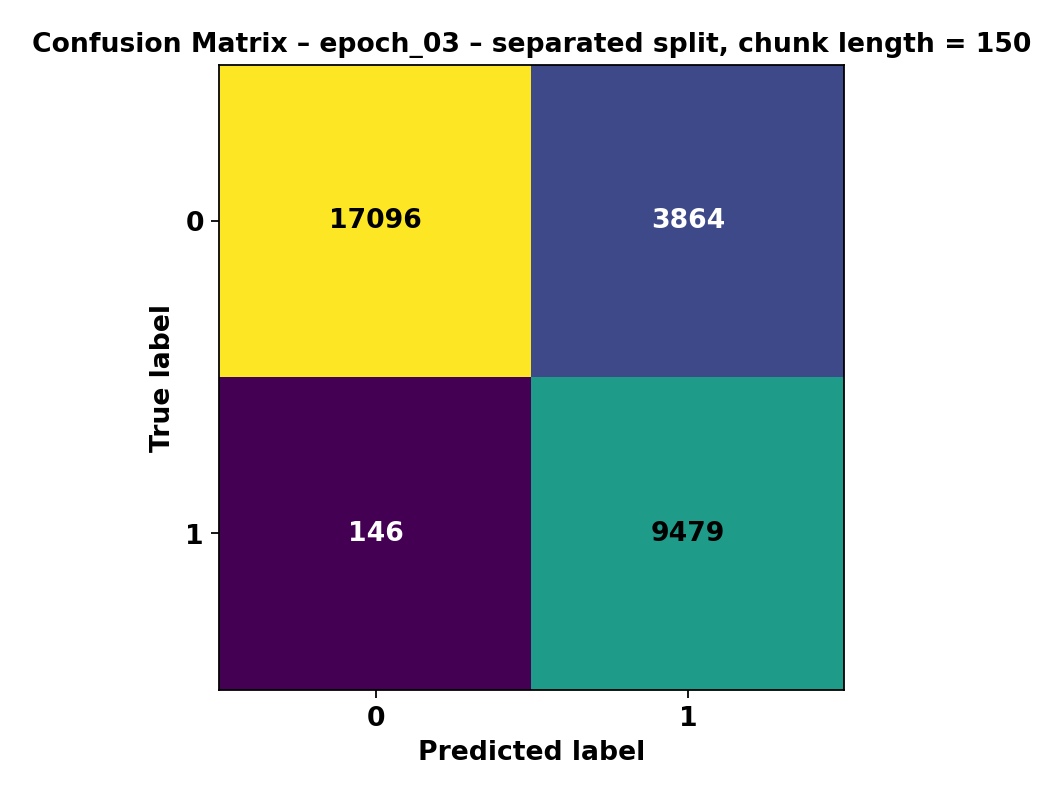
\includegraphics[width=\linewidth, trim={0 12 0 10},clip]{bert_baseline_plots/sep_synth_in_test/len150/confmat_epoch_03.png}
    \caption{Chunk size = 150 tokens}
  \end{subfigure}\hfill
  \begin{subfigure}[t]{0.32\textwidth}
    \centering
    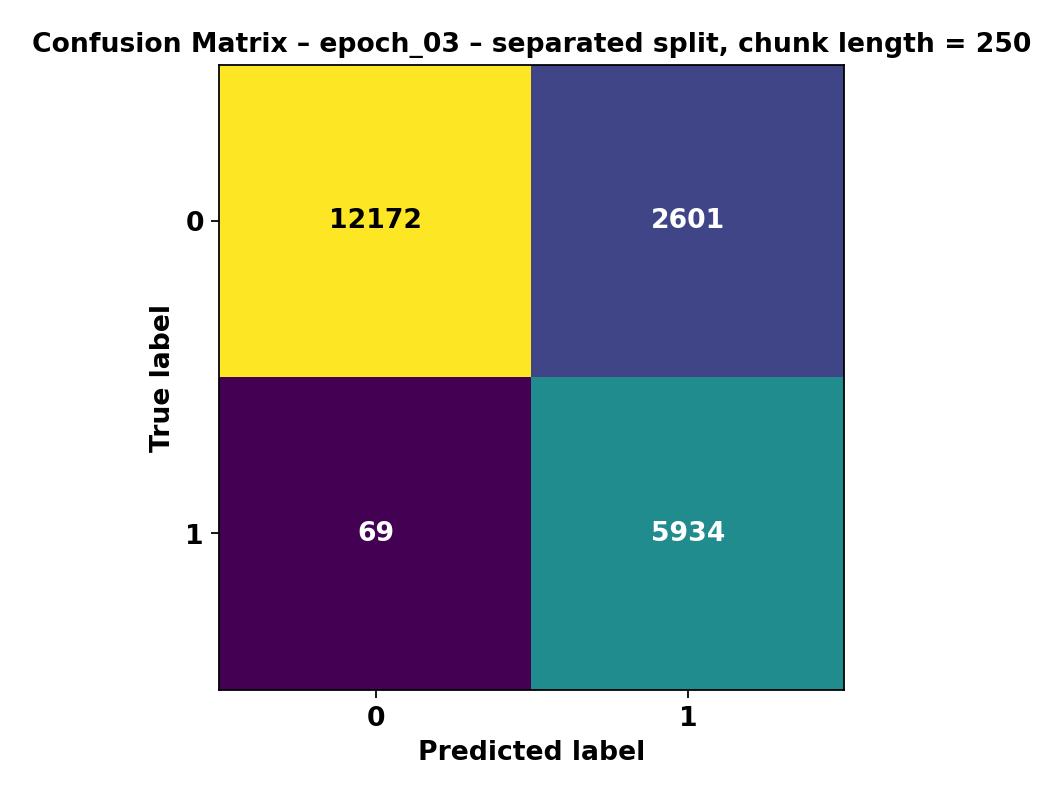
\includegraphics[width=\linewidth, trim={0 12 0 10},clip]{bert_baseline_plots/sep_synth_in_test/len250/confmat_epoch_03.png}
    \caption{Chunk size = 250 tokens}
  \end{subfigure}\hfill
  \begin{subfigure}[t]{0.32\textwidth}
    \centering
    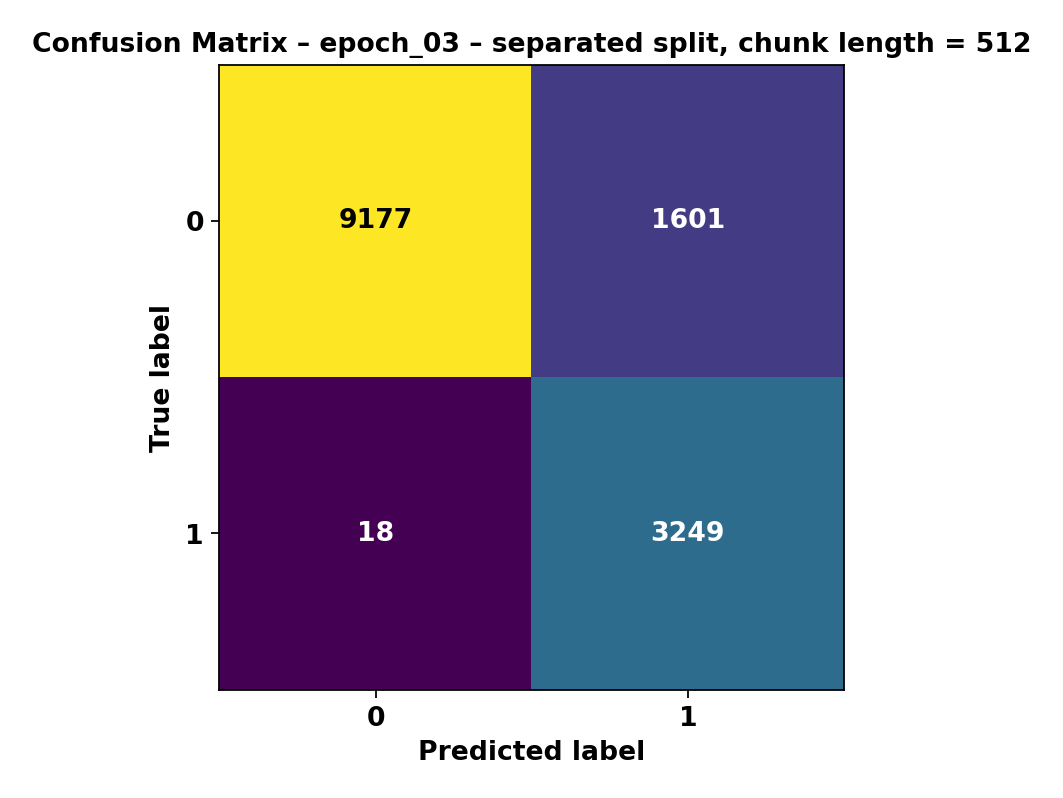
\includegraphics[width=\linewidth, trim={0 12 0 10},clip]{bert_baseline_plots/sep_synth_in_test/len512/confmat_epoch_03.png}
    \caption{Chunk size = 512 tokens}
  \end{subfigure}

  % --- Zweite Reihe: Train + Test-Synthetic ---
  \vspace{0.4cm}
  \begin{subfigure}[t]{0.32\textwidth}
    \centering
    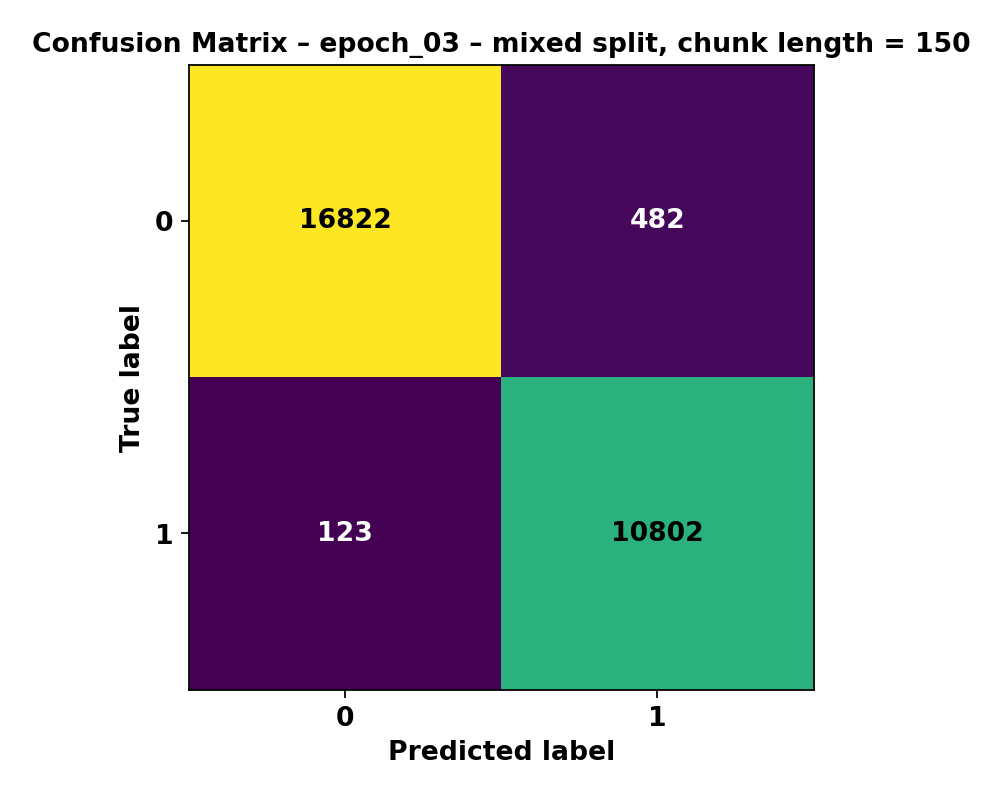
\includegraphics[width=\linewidth, trim={0 0 0 10},clip]{bert_baseline_plots/mixed/len150/confmat_epoch_03.png}
    \caption{Chunk size = 150 tokens}
  \end{subfigure}\hfill
  \begin{subfigure}[t]{0.32\textwidth}
    \centering
    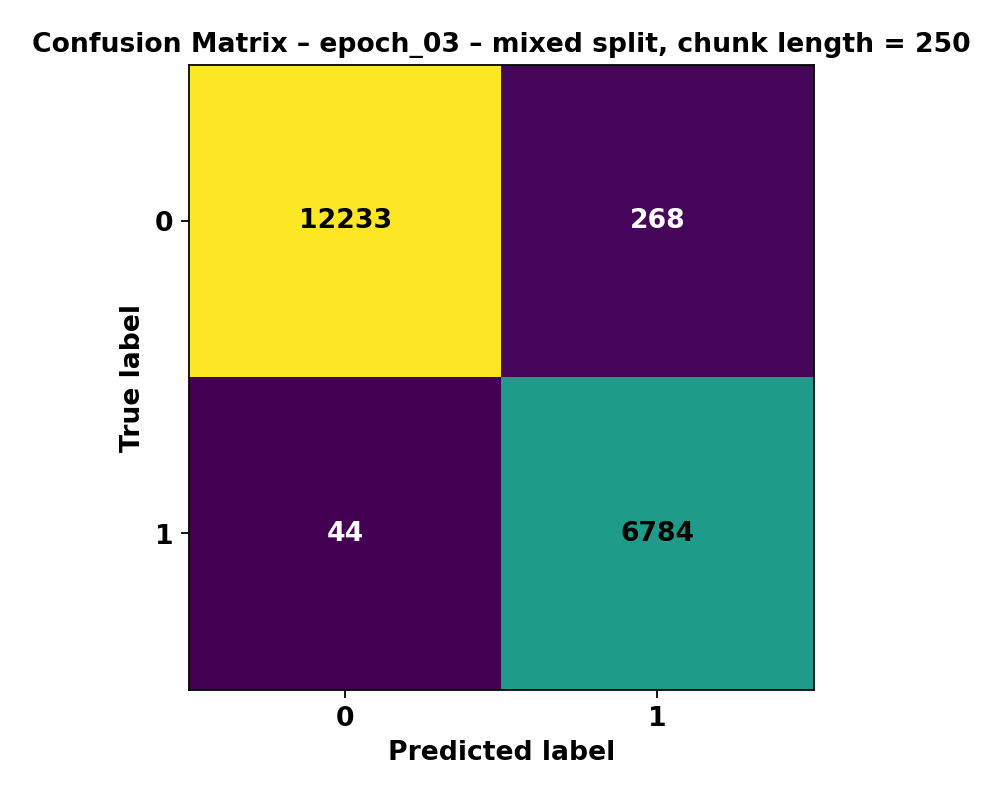
\includegraphics[width=\linewidth, trim={0 0 0 10},clip]{bert_baseline_plots/mixed/len250/confmat_epoch_03.png}
    \caption{Chunk size = 250 tokens}
  \end{subfigure}\hfill
  \begin{subfigure}[t]{0.32\textwidth}
    \centering
    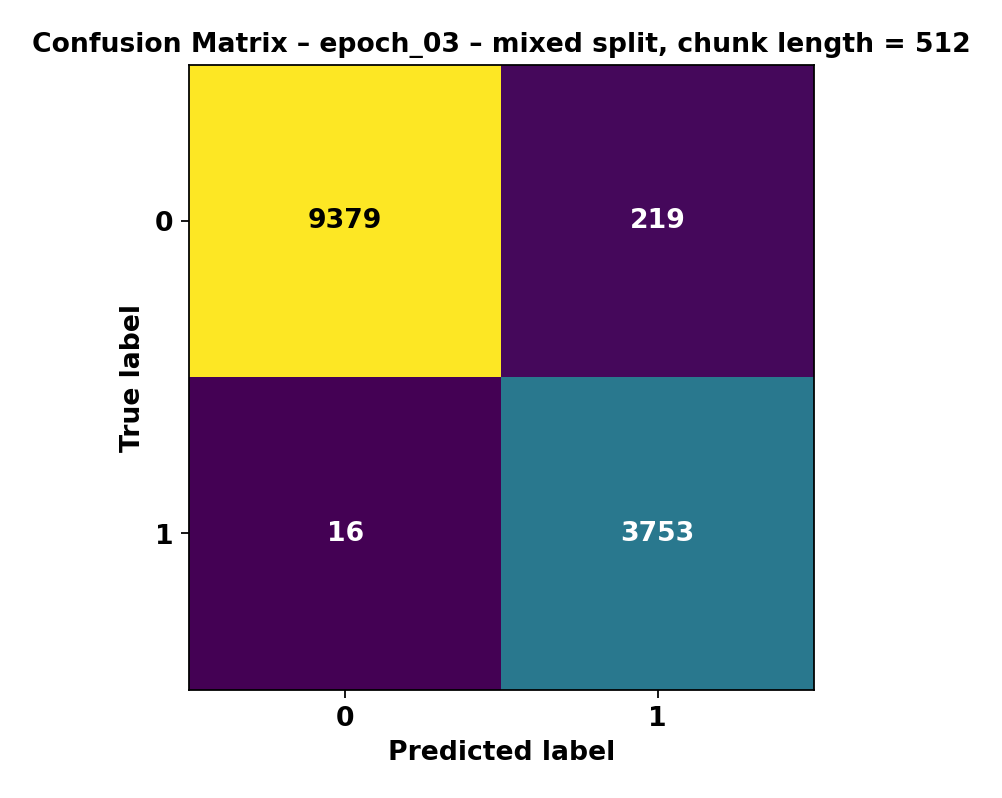
\includegraphics[width=\linewidth, trim={0 0 0 10},clip]{bert_baseline_plots/mixed/len512/confmat_epoch_03.png}
    \caption{Chunk size = 512 tokens}
  \end{subfigure}

  \caption[Confusion matrices of BERT baseline after epoch 3.]{\textbf{Confusion matrices of the BERT baseline after epoch 3.}  
  Top row: models trained with synthetic data included only in the test set.  
  Bottom row: models trained with synthetic data included in both train and test set.  
  Each column corresponds to a different chunk length (150, 250, 512).}
  \label{fig:bert_confusionmatrices_epoch3}
\end{figure}

Figure \ref{fig:bert_confusionmatrices_epoch3} shows the confusion matrices for the BERT baseline across different chunk sizes and dataset configurations after epoch 3. When looking at the chunk lengths, the false positives and false negatives decrease steadily with an increasing chunk size for both, the false positive and false negative rate and the mixed and seperated data setup. This indicates that the model benefits from a larger context and higher word count, which is consistent with the improved metrics observed in table \ref{tab:bert_base}. It is evident, that the model with the synthetic data in both train and test set achieves a clearly better performance across all chunk sizes with a distingtly lower false positive and also a slightly lower false negative rate across all chunk sizes. This confirms the earlier observation that including synthetic data in training helps the model generalize better to this distribution, leading to fewer misclassifications. 

What is the most striking, is the general higher false positive rate compared to the false negative rate across all configurations. Especially in the setup with the synthetic data only in the test set, the false positive rate is notably higher than the false negative rate (e.g. 1601 FP vs only 18 FN for chunk length 512 tokens), particularly for smaller chunk sizes (e.g. 3864 FP vs 146 FN for chunk length = 150 tokens). Even in the mixed setup, where the performance is generally better, the false positive rate remains slightly higher than the false negative rate. This indicates that the model is generally more conservative in its predictions, preferring to classify uncertain cases as grooming rather than risking missing actual grooming conversations. This behavior is often desirable in practical applications where false negatives (missed grooming cases) can have serious consequences. As already mentioned, the dataset is very balanced, which also contributes to the low false negative rates. Overall, the confusion matrices confirm that BERT performs very well across all configurations, with performance improving with larger chunk sizes and when synthetic data is included in training and with the best performance for chunk size 512 and mixed data setup. \textbf{Note that the values for accuracy, precision and f1 scores are still lower for the mixed setup with chunk size of 512 tokens compared to the mixed setup with chunk size of 250 tokens in table \ref{tab:bert_base}.} This happens because the dataset for 512-token chunks contains fewer samples overall. While the absolute number of false positives and false negatives is lower, their relative share among predictions is higher, which reduces precision. At the same time, recall slightly improves since almost no true positives are missed.


\subsection{ROC Curves for BERT Baseline across Chunk Sizes and Data Setups}

%%%%%%% ROC CURVES

\begin{figure}[H]
  \centering

  % ---------- Top row: synthetic only in TEST ----------
  \begin{subfigure}[t]{0.32\textwidth}
    \centering
    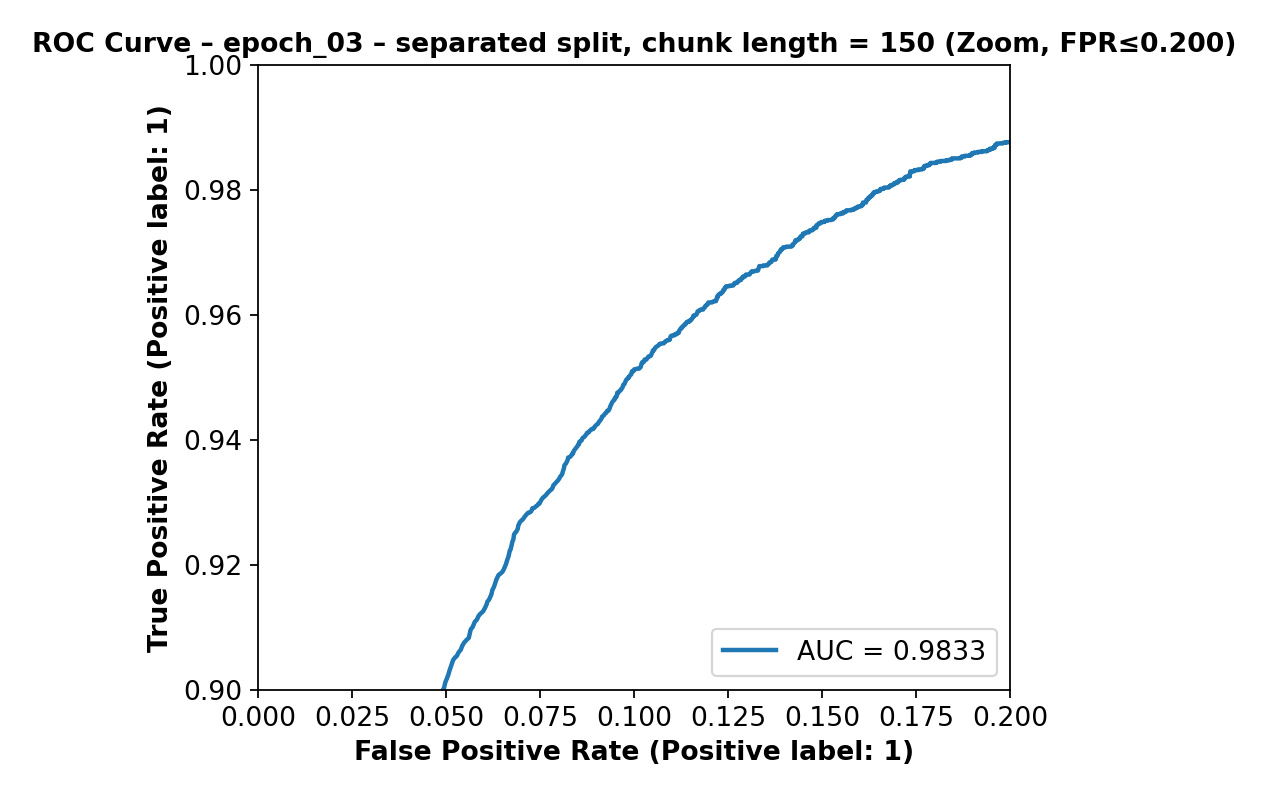
\includegraphics[width=\linewidth]{bert_baseline_plots/sep_synth_in_test/len150/roc_epoch_03_zoom.png}
    \caption{Chunk length = 150}
  \end{subfigure}\hfill
  \begin{subfigure}[t]{0.32\textwidth}
    \centering
    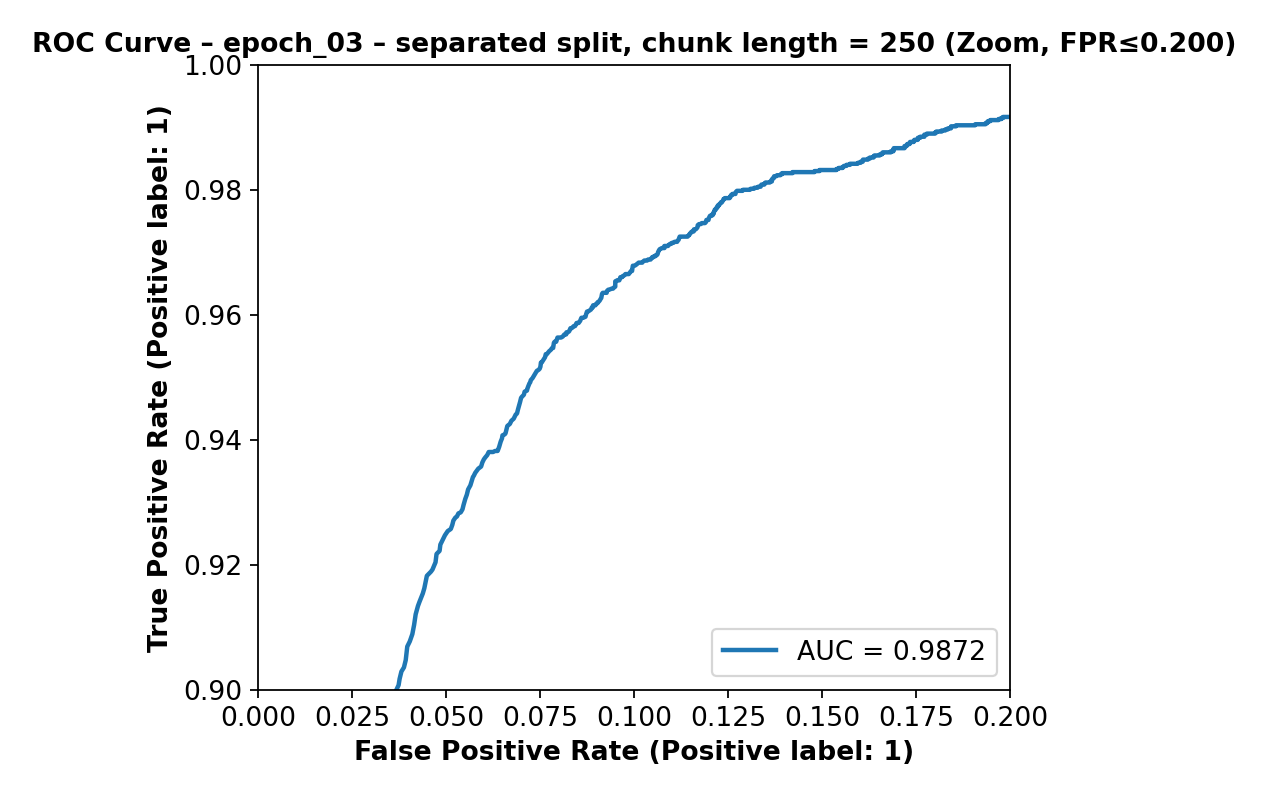
\includegraphics[width=\linewidth]{bert_baseline_plots/sep_synth_in_test/len250/roc_epoch_03_zoom.png}
    \caption{Chunk length = 250}
  \end{subfigure}\hfill
  \begin{subfigure}[t]{0.32\textwidth}
    \centering
    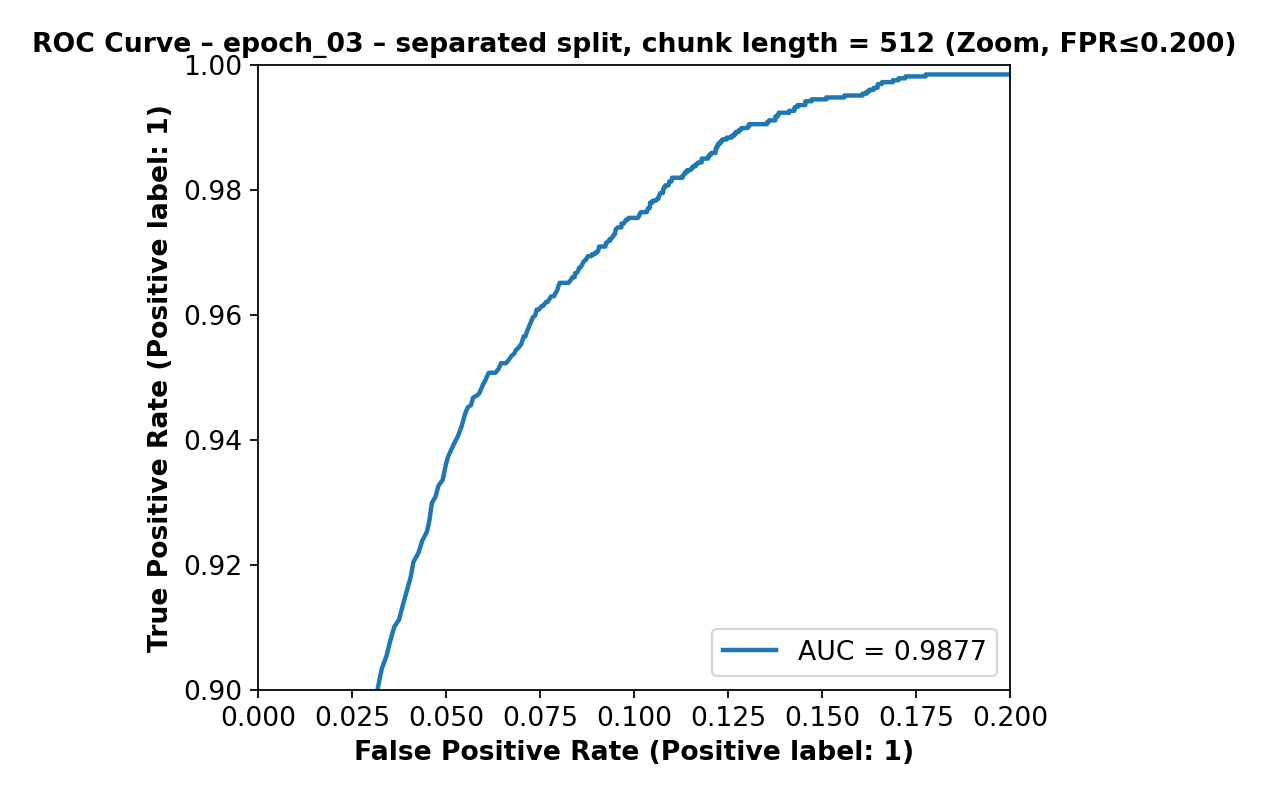
\includegraphics[width=\linewidth]{bert_baseline_plots/sep_synth_in_test/len512/roc_epoch_03_zoom.png}
    \caption{Chunk length = 512}
  \end{subfigure}

  % ---------- Bottom row: synthetic in TRAIN & TEST ----------
  \vspace{0.45cm}
  \begin{subfigure}[t]{0.32\textwidth}
    \centering
    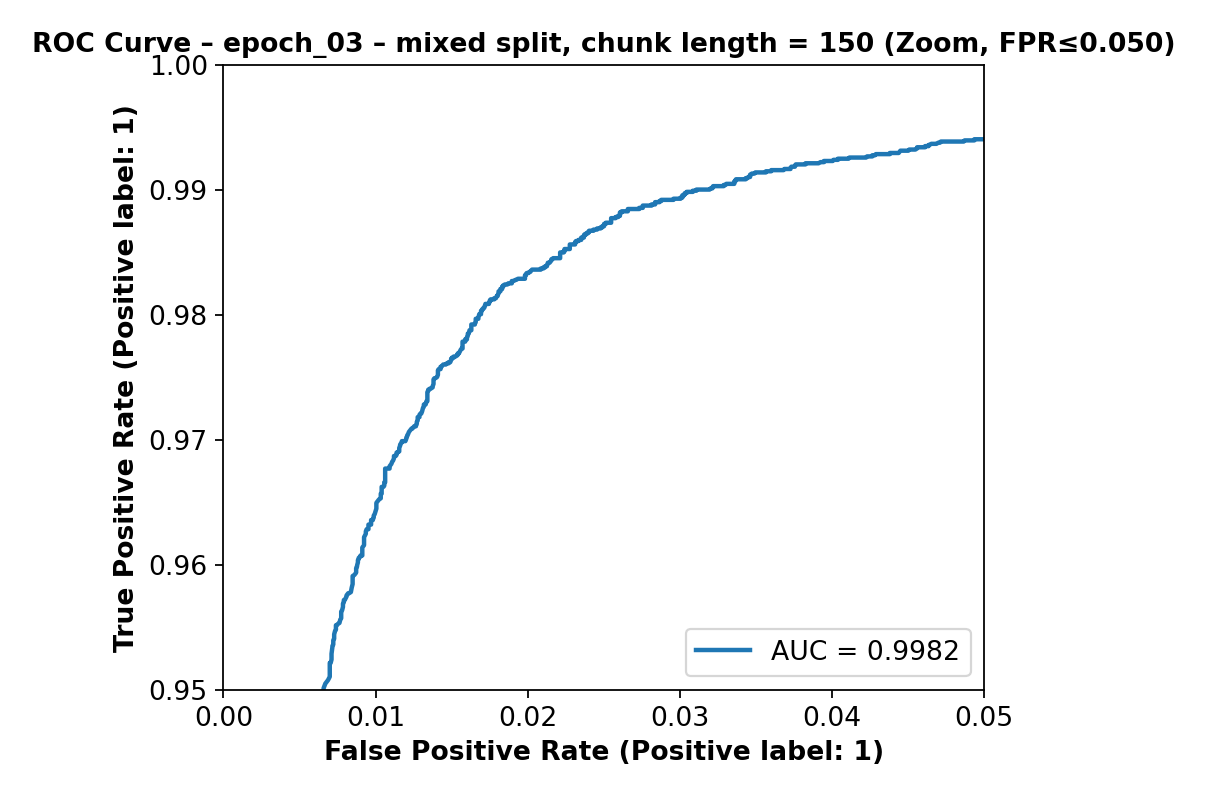
\includegraphics[width=\linewidth]{bert_baseline_plots/mixed/len150/roc_epoch_03_zoom.png}
    \caption{Chunk length = 150}
  \end{subfigure}\hfill
  \begin{subfigure}[t]{0.32\textwidth}
    \centering
    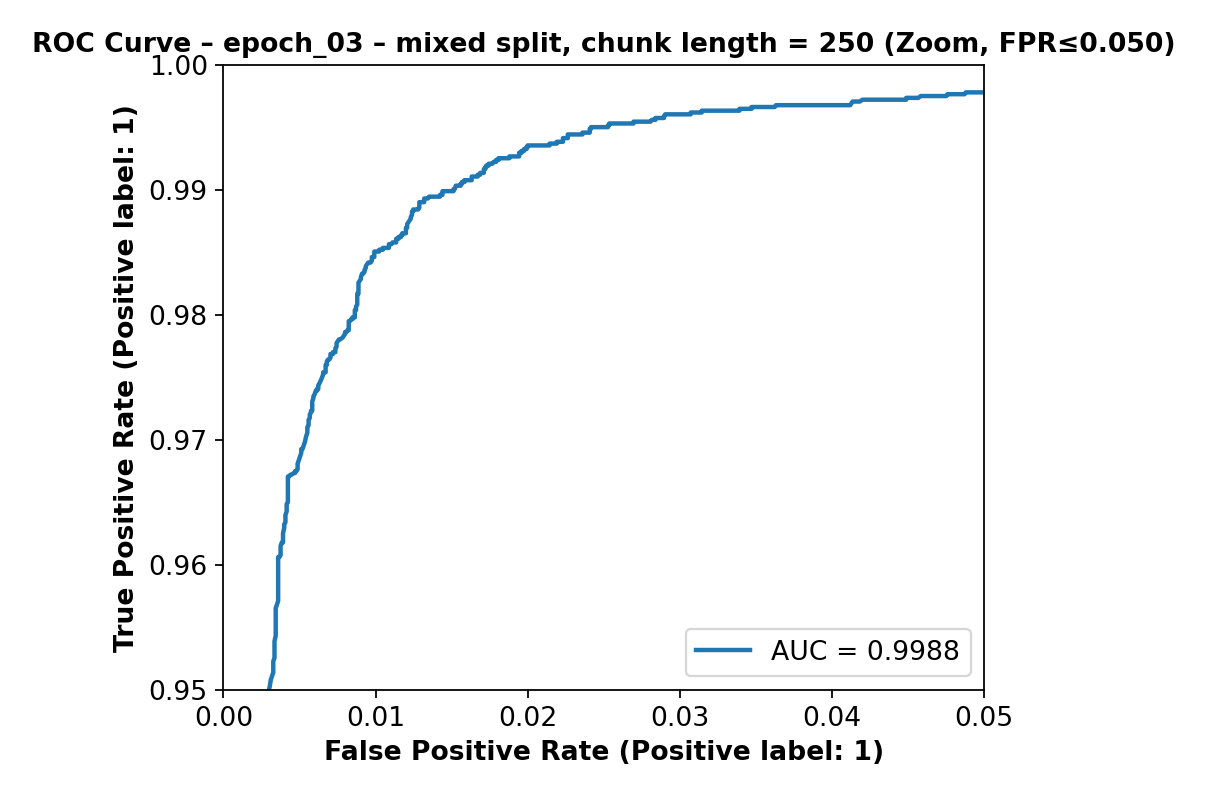
\includegraphics[width=\linewidth]{bert_baseline_plots/mixed/len250/roc_epoch_03_zoom.png}
    \caption{Chunk length = 250}
  \end{subfigure}\hfill
  \begin{subfigure}[t]{0.32\textwidth}
    \centering
    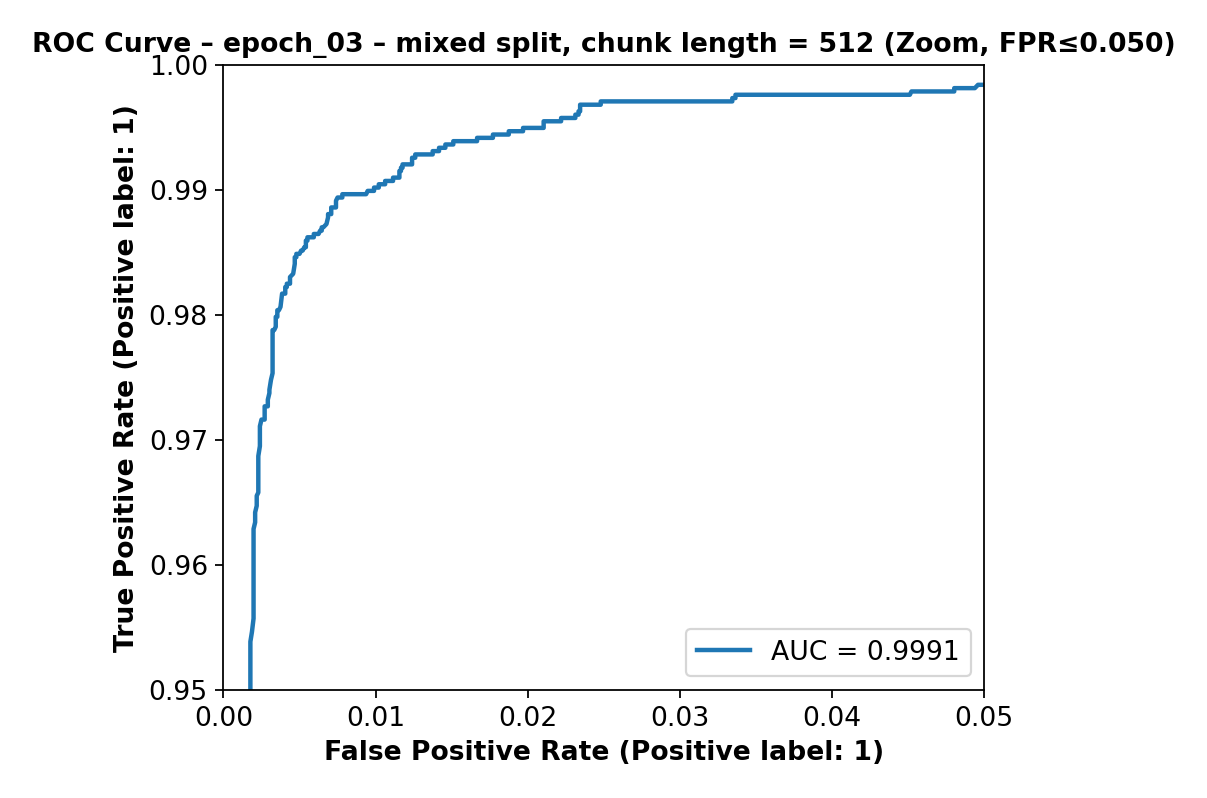
\includegraphics[width=\linewidth]{bert_baseline_plots/mixed/len512/roc_epoch_03_zoom.png}
    \caption{Chunk length = 512}
  \end{subfigure}

  \caption[Zoomed ROC curves after epoch 3 for different chunk lengths.]{\textbf{Zoomed ROC curves after epoch 3 for different chunk lengths (BERT baseline).}
  Top row: models evaluated with synthetic data included \emph{only in the test set} (\(\mathrm{False Positive Rate}\le 0.20\) and \(\mathrm{TPR}\ge 0.90\)). 
  Bottom row: models trained and evaluated with synthetic data in \emph{train \& test} and therefore shown with a \emph{tighter zoom} to expose finer differences (\(\mathrm{False Positive Rate}\le 0.05\) and \(\mathrm{TPR}\ge 0.95\)). 
  Each panel shows the zoomed range of the ROC curve to better reveal separation at low false-positive rates; the legend reports the pAUC for the full ROC.}
  \label{fig:roc_zoom_epoch3}
\end{figure}

Figure \ref{fig:roc_zoom_epoch3} shows the zoomed ROC curves for the BERT baseline across different chunk sizes and dataset configurations after epoch 3. The ROC curves were plotted zoomed for both configurations to highlight the differences more clearly, as the model already performed very well, especially for the mixed dataset, with small differences in the F1 score of < 1\% after epoch 3. \textbf{Note that the zoom levels differ between the two setups.For the setup with synthetic data only in the test set, the ROC curves are shown with a zoom on false positive rates ≤ 0.20 and true positive rates ≥ 0.90, highlighting the overall performance at moderately low FPRs where differences between chunk sizes are still relatively small. For the mixed data setup, a stronger zoom was applied (FPR ≤ 0.05, TPR ≥ 0.95) to emphasize finer distinctions between the models in the critical region, where even small errors become relevant.} 

When looking at the chunk lengths, it is evident that the ROC curves improve steadily with increasing chunk size for both configurations. This indicates that the model benefits from a larger context and higher word count, which is consistent with the improved metrics observed in table \ref{tab:bert_base} and the confusion matrices in figure \ref{fig:bert_confusionmatrices_epoch3}. The pAUC values also increase with chunk size, confirming that larger chunks lead to better overall discrimination between grooming and non-grooming conversations. When comparing the pAUC scores between the two configurations, it is clear that the models trained with synthetic data in both train and test sets achieve significantly higher pAUC values across all chunk sizes. This confirms the earlier observation that including synthetic data in training helps the model generalize better to this distribution, leading to improved performance across the entire ROC curve. Overall, the zoomed ROC curves confirm that BERT performs very well across all configurations, with performance improving with larger chunk sizes and when synthetic data is included in training, consistent with previous analyses.

\section{Comparing LIWC-2022 Macro Groups} \label{sec:global_liwc_analysis}


\begin{figure}[ht]
    \centering
    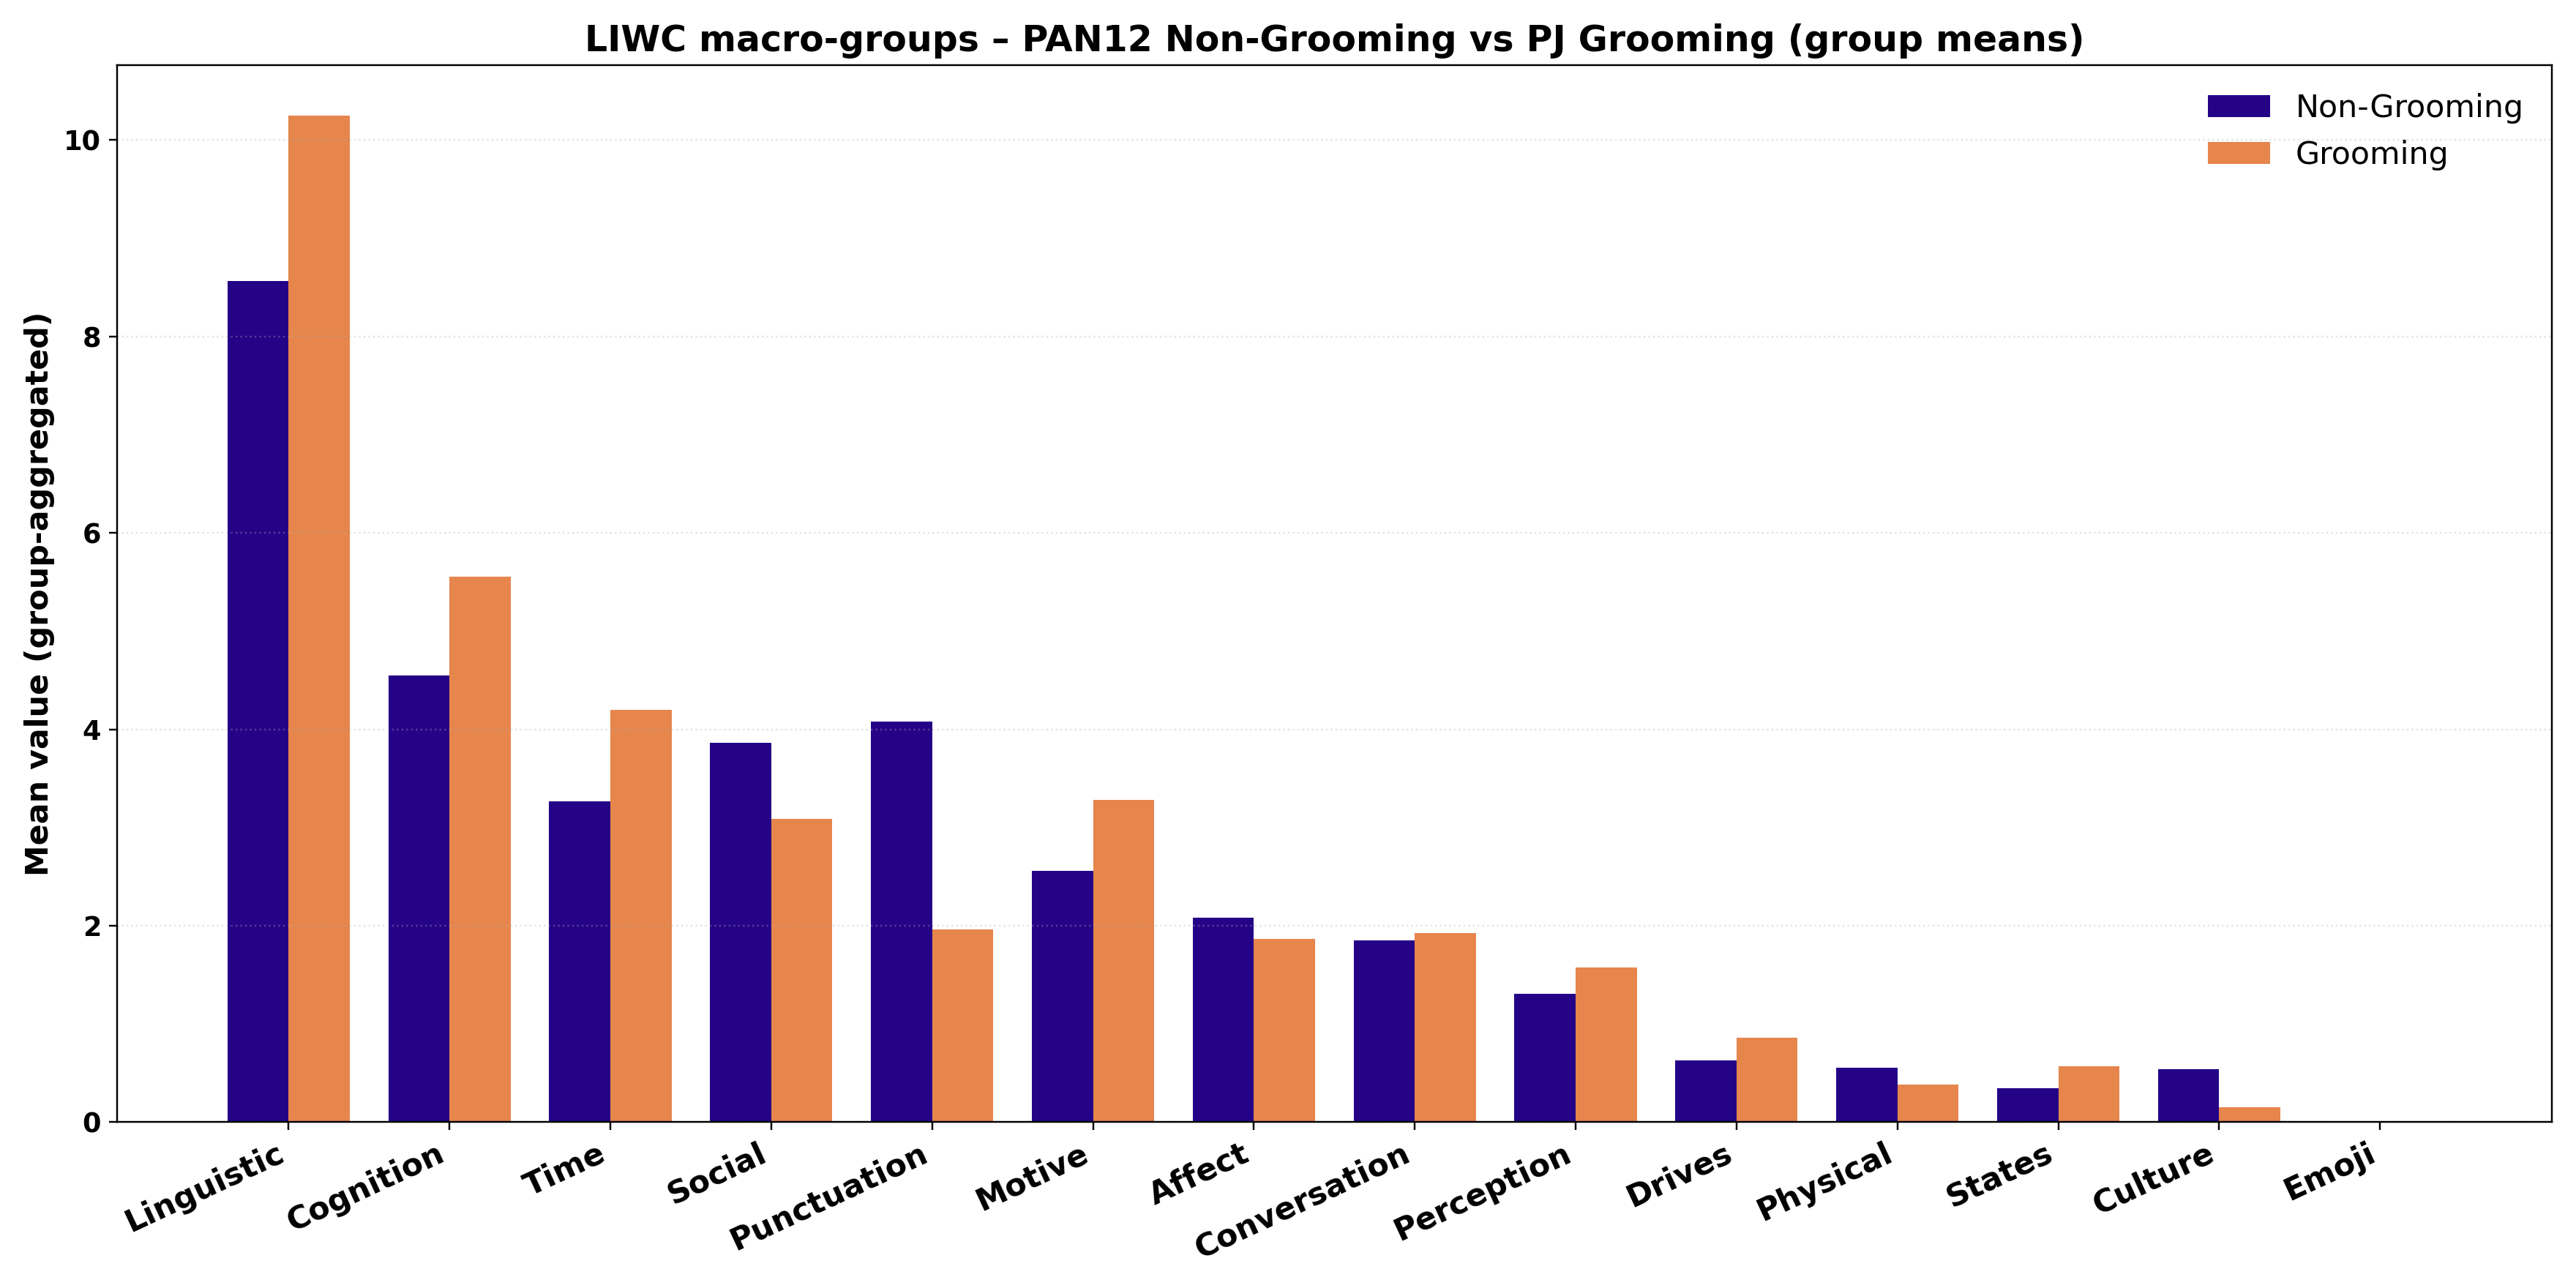
\includegraphics[width=0.90\textwidth]{groups_mean_pan12_vs_pj.png}
    \caption[Comparison of aggregated LIWC macro-groups]{Comparison of aggregated LIWC macro-groups between PAN12 (non-grooming) and PJ (grooming) over global conversations.}
    \label{fig:liwc_macro_groups}
\end{figure}


Figure~\ref{fig:liwc_macro_groups} compares the mean values between the LIWC scores of PAN12 (non-grooming) and PJ (grooming) conversations, aggregated into their Macro Groups.

The results indicate that linguistic features dominate both corpora, with PJ showing significant higher values. \textit{Note that the collected PJ conversations are generally longer and therefore containing more linguistic markers overall.} More interesting is, that the groups \textit{Time}, \textit{Cognition} and \textit{Social} stand out, where PJ conversations show a stronger presence of temporal references (often linked to future planning of meetings), cognitive processes and social markers. Also, the Category ``Emoji´´ hows no Liwc-Values for both Datasets as a result of the slang handling and data preprocssing steps and different kind of emoji usage in the time, the datasets were collected.

Overall, the group-level aggregation highlights the major shifts across all LIWC-dimensions, providing a perspective to the category-wise analysis. This confirms that grooming communication is  characterized not only by increased length and density of language, but also by a distinct emphasis on cognitive, temporal and social processes.


\section{Comparing LIWC Features between PJ and PAN12 on Full Conversations} \label{sec:liwc_global_analysis}

\begin{figure}[ht]
    \centering
    \begin{subfigure}[t]{0.48\textwidth}
        \centering
        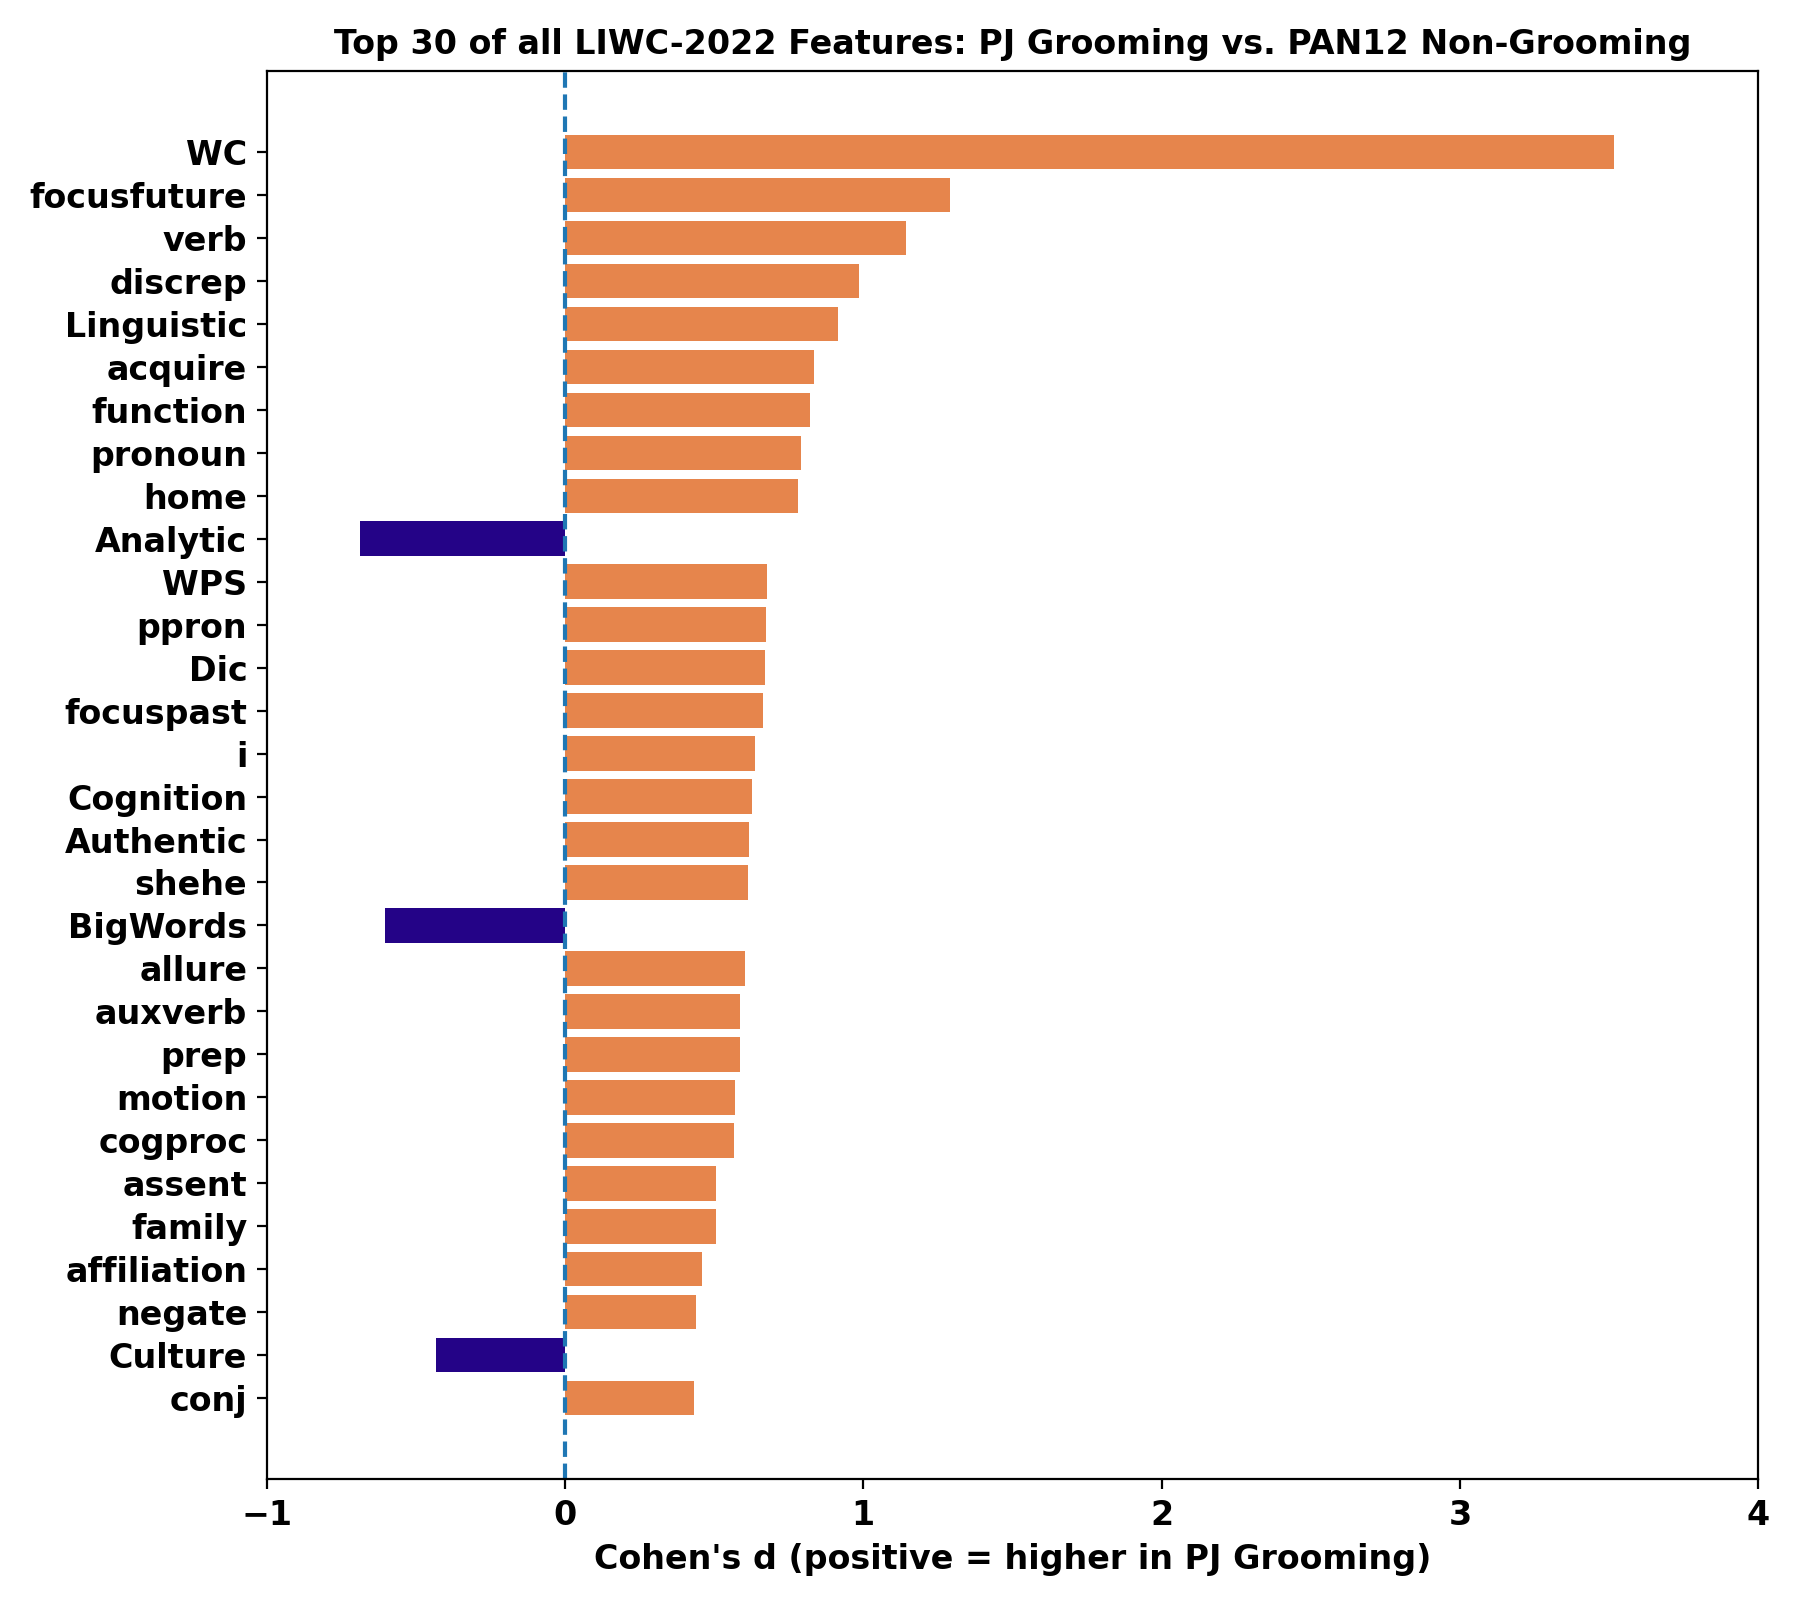
\includegraphics[width=\linewidth]{liwc_top15_d_global.png}
        \caption{Top 30 LIWC categories across all LIWC-2022 features.}
    \end{subfigure}
    \hfill
    \begin{subfigure}[t]{0.48\textwidth}
        \centering
        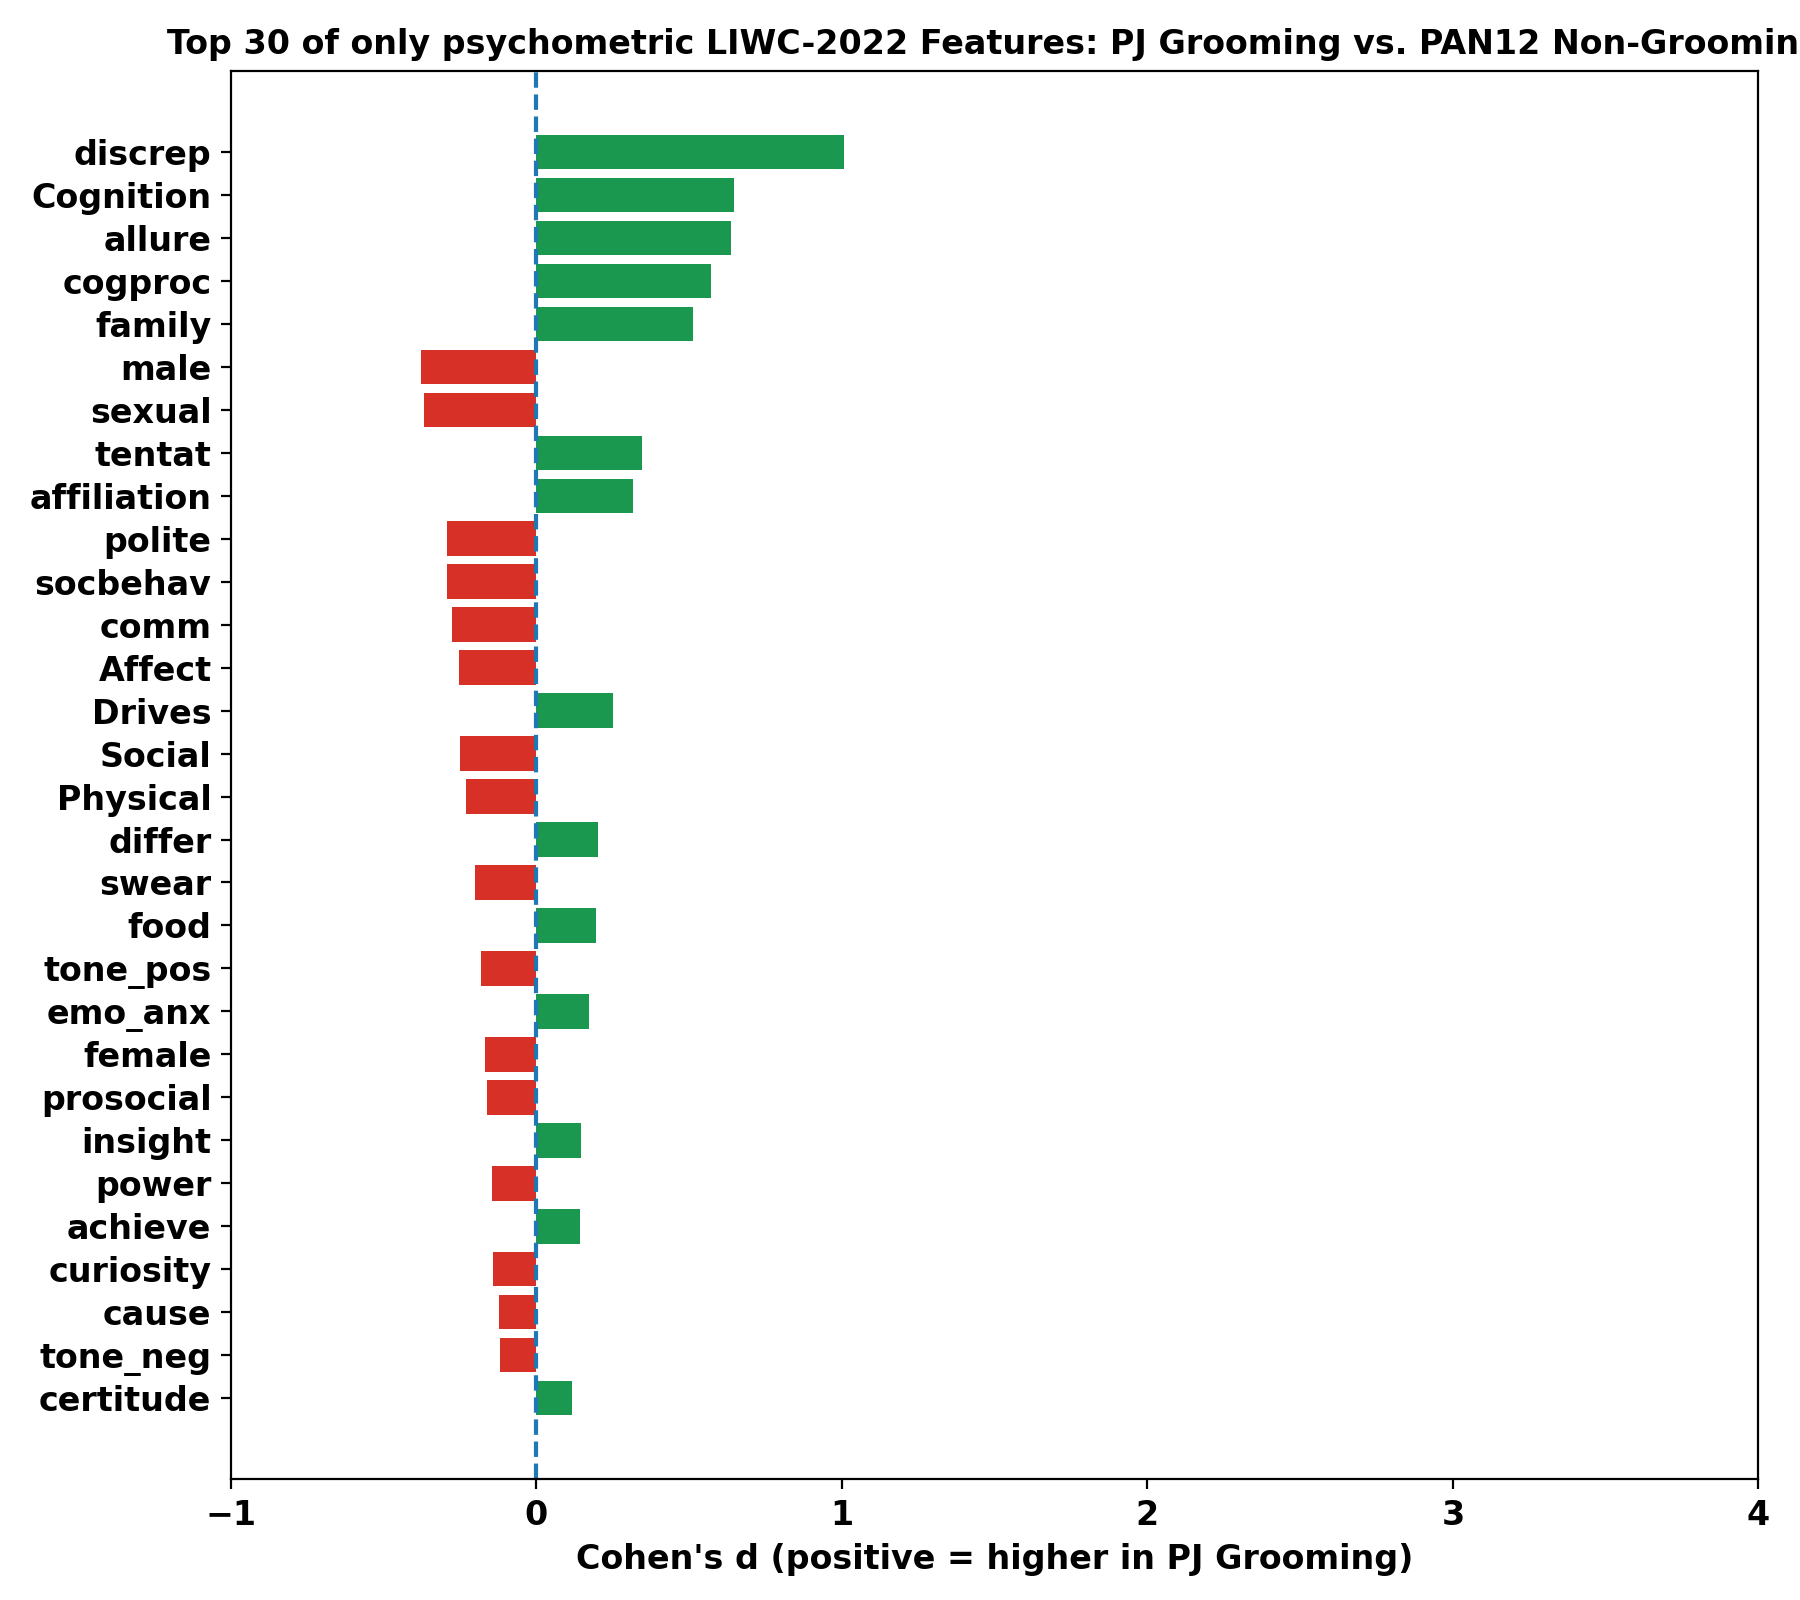
\includegraphics[width=\linewidth]{liwc_top15_d_by_psychometrics.png}
        \caption{Top 30 LIWC-2022 features highlighted in the literature.}
    \end{subfigure}
    \caption[LIWC feature Comparison (PJ, PAN12) over Complete Conversations]{LIWC feature comparison between grooming (PJ) and non-grooming (PAN12) dialogues based on cohens $d$ \cite{cohen1988}. Positive values indicate higher feature usage in grooming.}
    \label{fig:liwc_global_analysis}
\end{figure}


In addition, the effect size \textbf{Cohen’s $d$} \cite{cohen1988} was computed to quantify group differences. Figure \ref{fig:liwc_global_analysis} (left) shows the top 30 LIWC features with the largest absolute effect sizes across all LIWC-2022 features, while figure \ref{fig:liwc_global_analysis} (right) focuses on the top 30 features from the psychometric subset highlighted in prior literature (Section \ref{sec:liwc-feature-selection}). For both plots, values over 0 indicate higher feature values in PJ-Grooming conversations, while values below 0 indicate higher values in PAN12 non-grooming conversations. Note, that effect sizes appear lower in the psychometric subset, since it is fully contained within the complete feature set and does not include the strongest differentiating features as shown in the left figure. 

Again, as shown in figure~\ref{fig:liwc_global_analysis} (left), PJ conversations are overall much longer (higher word counts), have longer sentences, and have overall more linguistically features like pronouns, verbs and function words. Since that is a strong confounder, for more content-related interpretations, these features should be ignored. When looking at the dialogical style, many functions words seem to be more prevalent in grooming conversations, which could be related to the more complex sentence structures and higher word counts. Also, the higher word count makes the pj conversations caputure a broader range of topics leading to more diverse linguistic markers.
What is noticeable is the strong presence of the feature \textit{focusfuture}, which reflects the grooming strategy of planning future meetings. Also, next to the linguistic features, the thematic references like \textit{family}, \textit{home} and \textit{affiliation} stand out, being higher present in grooming conversations from PJ than in PAN12, which could also be more consistent with the typical grooming narratives (e.g. asking, if the parents are home). Furthermore, the complexity in grooming conversations tends to be lower than in non-grooming conversations, as indicated by the lower \textit{big words}, \textit{Analytic} and \textit{Culture} score, which could be due to the sources that PAN12 was collected from (e.g. forums, chatrooms) which often containing computer-related and more complex language.

When focusing on the psychometric features (right), the differences between grooming and non-grooming conversations become more pronounced. It is noticeable, that grooming conversations show a higher values in features like \textit{Cogntition}, \textit{cognitive processes} and \textit{Allure} which could be caused by a content related reference to seduction and manipulation. Therefore grooming conversations are clearly distinguishable based on psychological strategies like building closeness (social/affilation), attraction (allure) and cognitive engagement (cognitive processes). Also, the strongest signal of grooming conversations lies in the feature \textit{discrep} (would, should, could), showing a higher presence of words which might be used in boundary testing, conditioning and suggestions. This is accompanied by slight positive effects for \textit{tentant} (hedging) and \textit{polite} (courtesy or relationship building). Additionally, the features \textit{Drives}, \textit{insight}, \textit{achieve} and \textit{emotion anxiety} are more prevalent in grooming conversations, which could be related to the manipulative strategies used by groomers to build trust and emotional connection.
It is striking, that the PAN12 Conversations contain higher values in the features \textit{sexual}, \textit{male/female}, \textit{physical}, \textit{swear} and \textit{Social/social behavior/prosocial}. This is likely due to the fact that the PAN12 dataset contains a considerable amount of sexually explicit but non-grooming conversations for which were included to improve model-robustness. \textbf{Because LIWC computes scores as relative proportions, the shorter PAN12 conversations, which often consist almost entirely of sexual content, produce inflated values in sexual-related categories. In comparison, the longer and more diverse PJ logs dilute these terms within a broader linguistic context, leading to lower proportional scores.} Therefore it should be considered, that the PAN12 dataset is not a perfect representation of non-grooming conversations, but rather a challenging counterbalance to the grooming data. Overall, the LIWC analysis confirms that grooming conversations are characterized not only by increased length and density of language, but also by a distinct emphasis on cognitive, temporal and social processes, as well as specific psychological strategies related to manipulation and relationship building. These insights provide a deeper understanding of the linguistic and psychological markers of grooming behavior, which can inform the development of more effective detection models.


\section{Comparing LIWC Features between PJ and PAN12 and the Synthetic Dataset} \label{sec:liwc_synthetic_comparison}
% Im Text
\begin{figure}[ht]
  \centering
  \begin{subfigure}[t]{0.48\textwidth}
    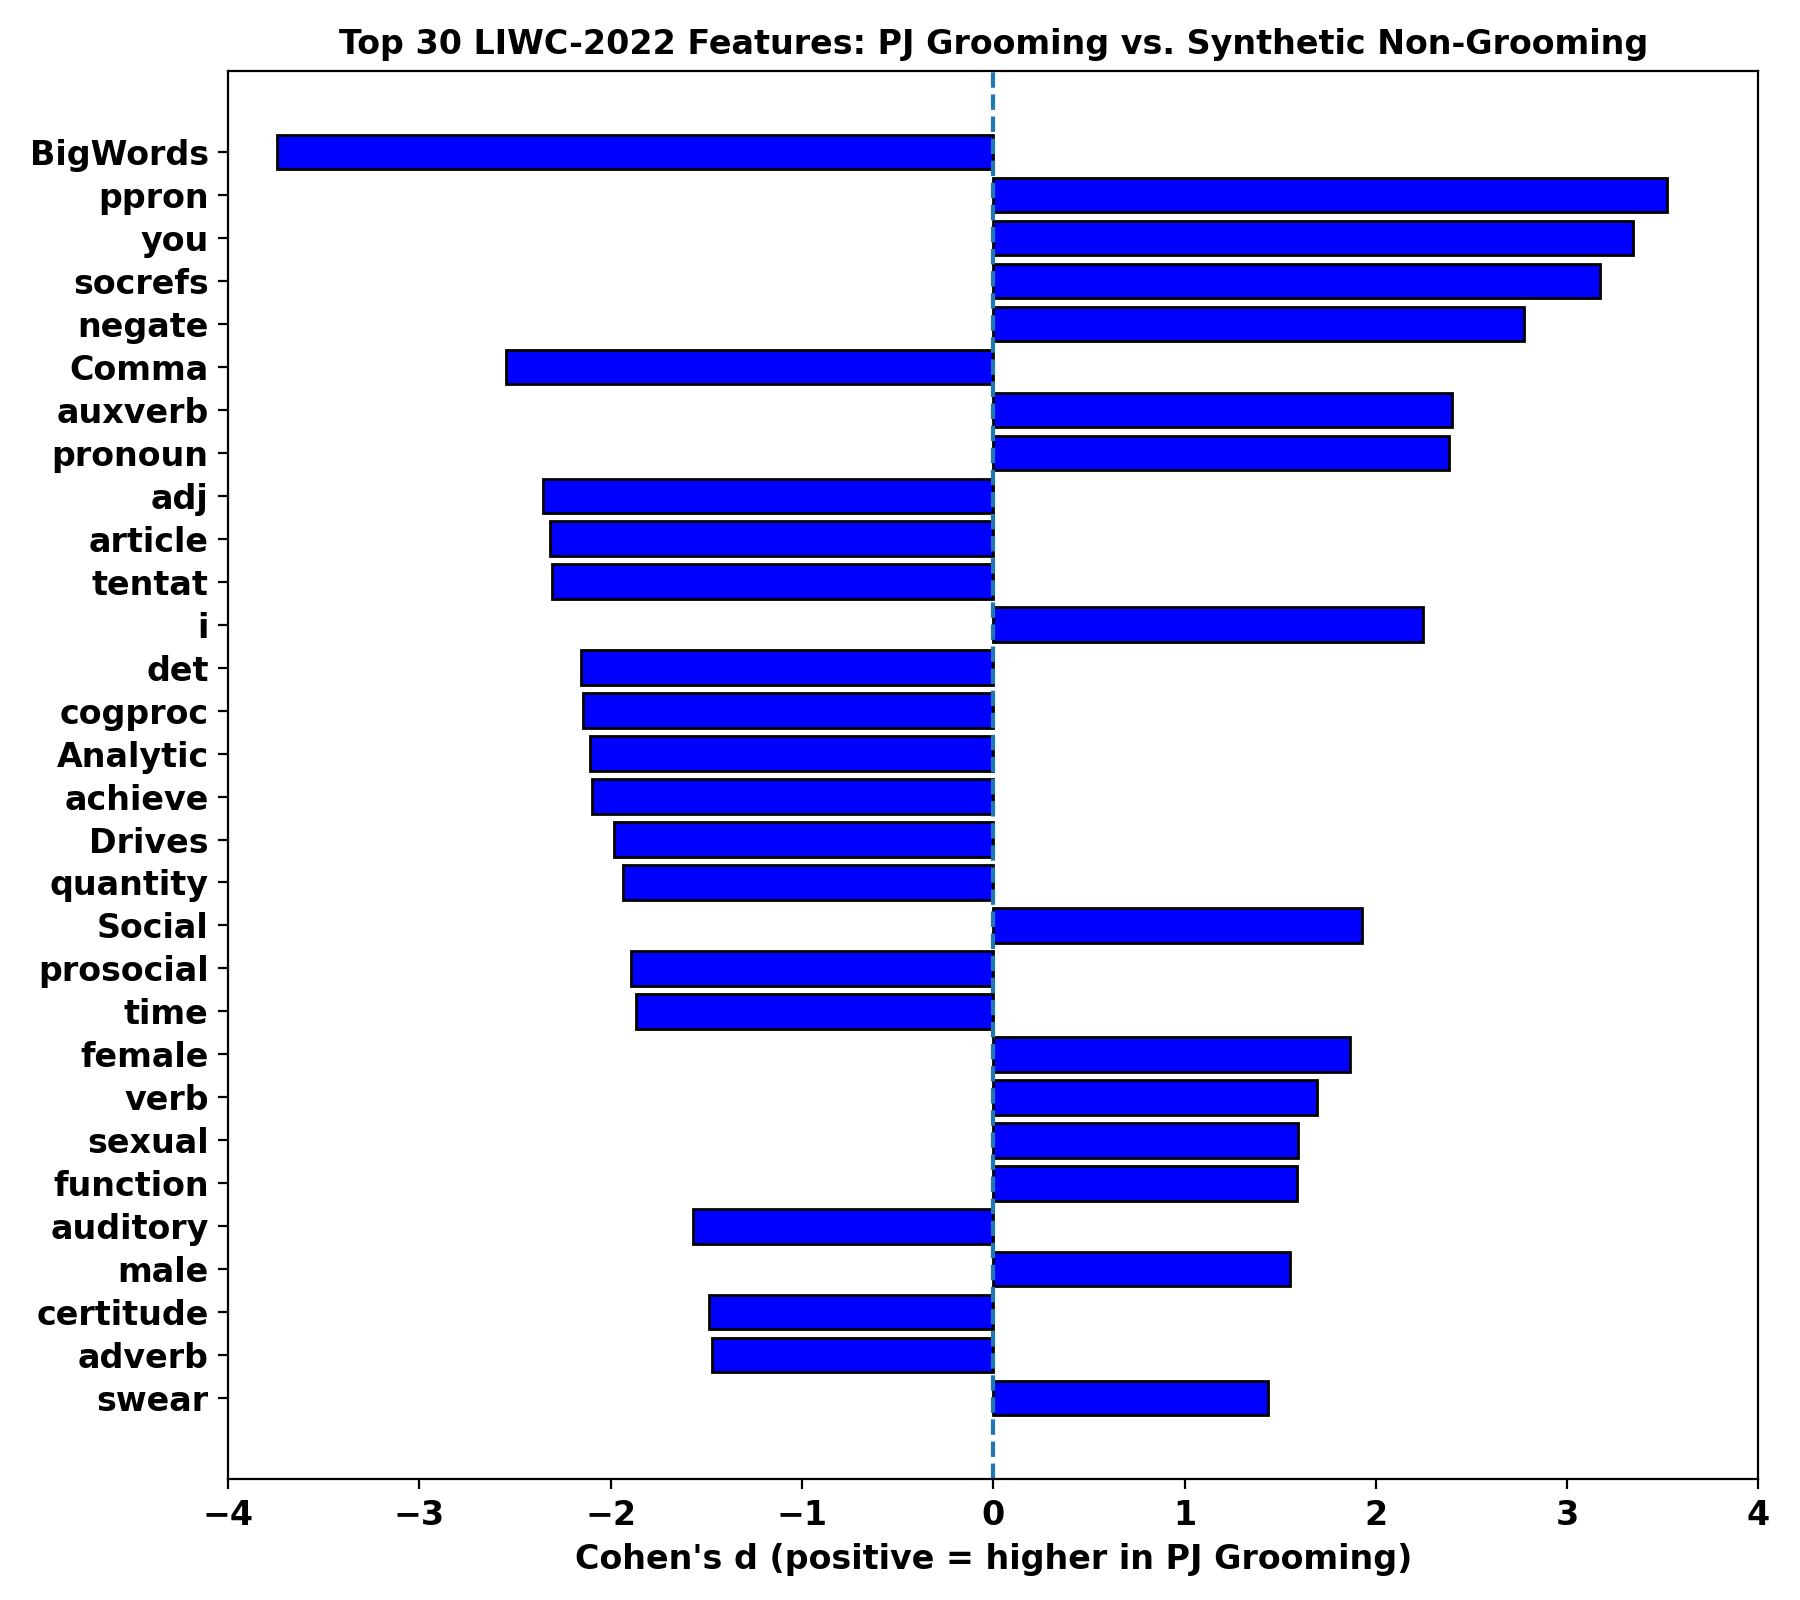
\includegraphics[width=\linewidth]{synthetic_comparison_pj.png}
    \caption{PJ vs. synthetic}
  \end{subfigure}\hfill
  \begin{subfigure}[t]{0.48\textwidth}
    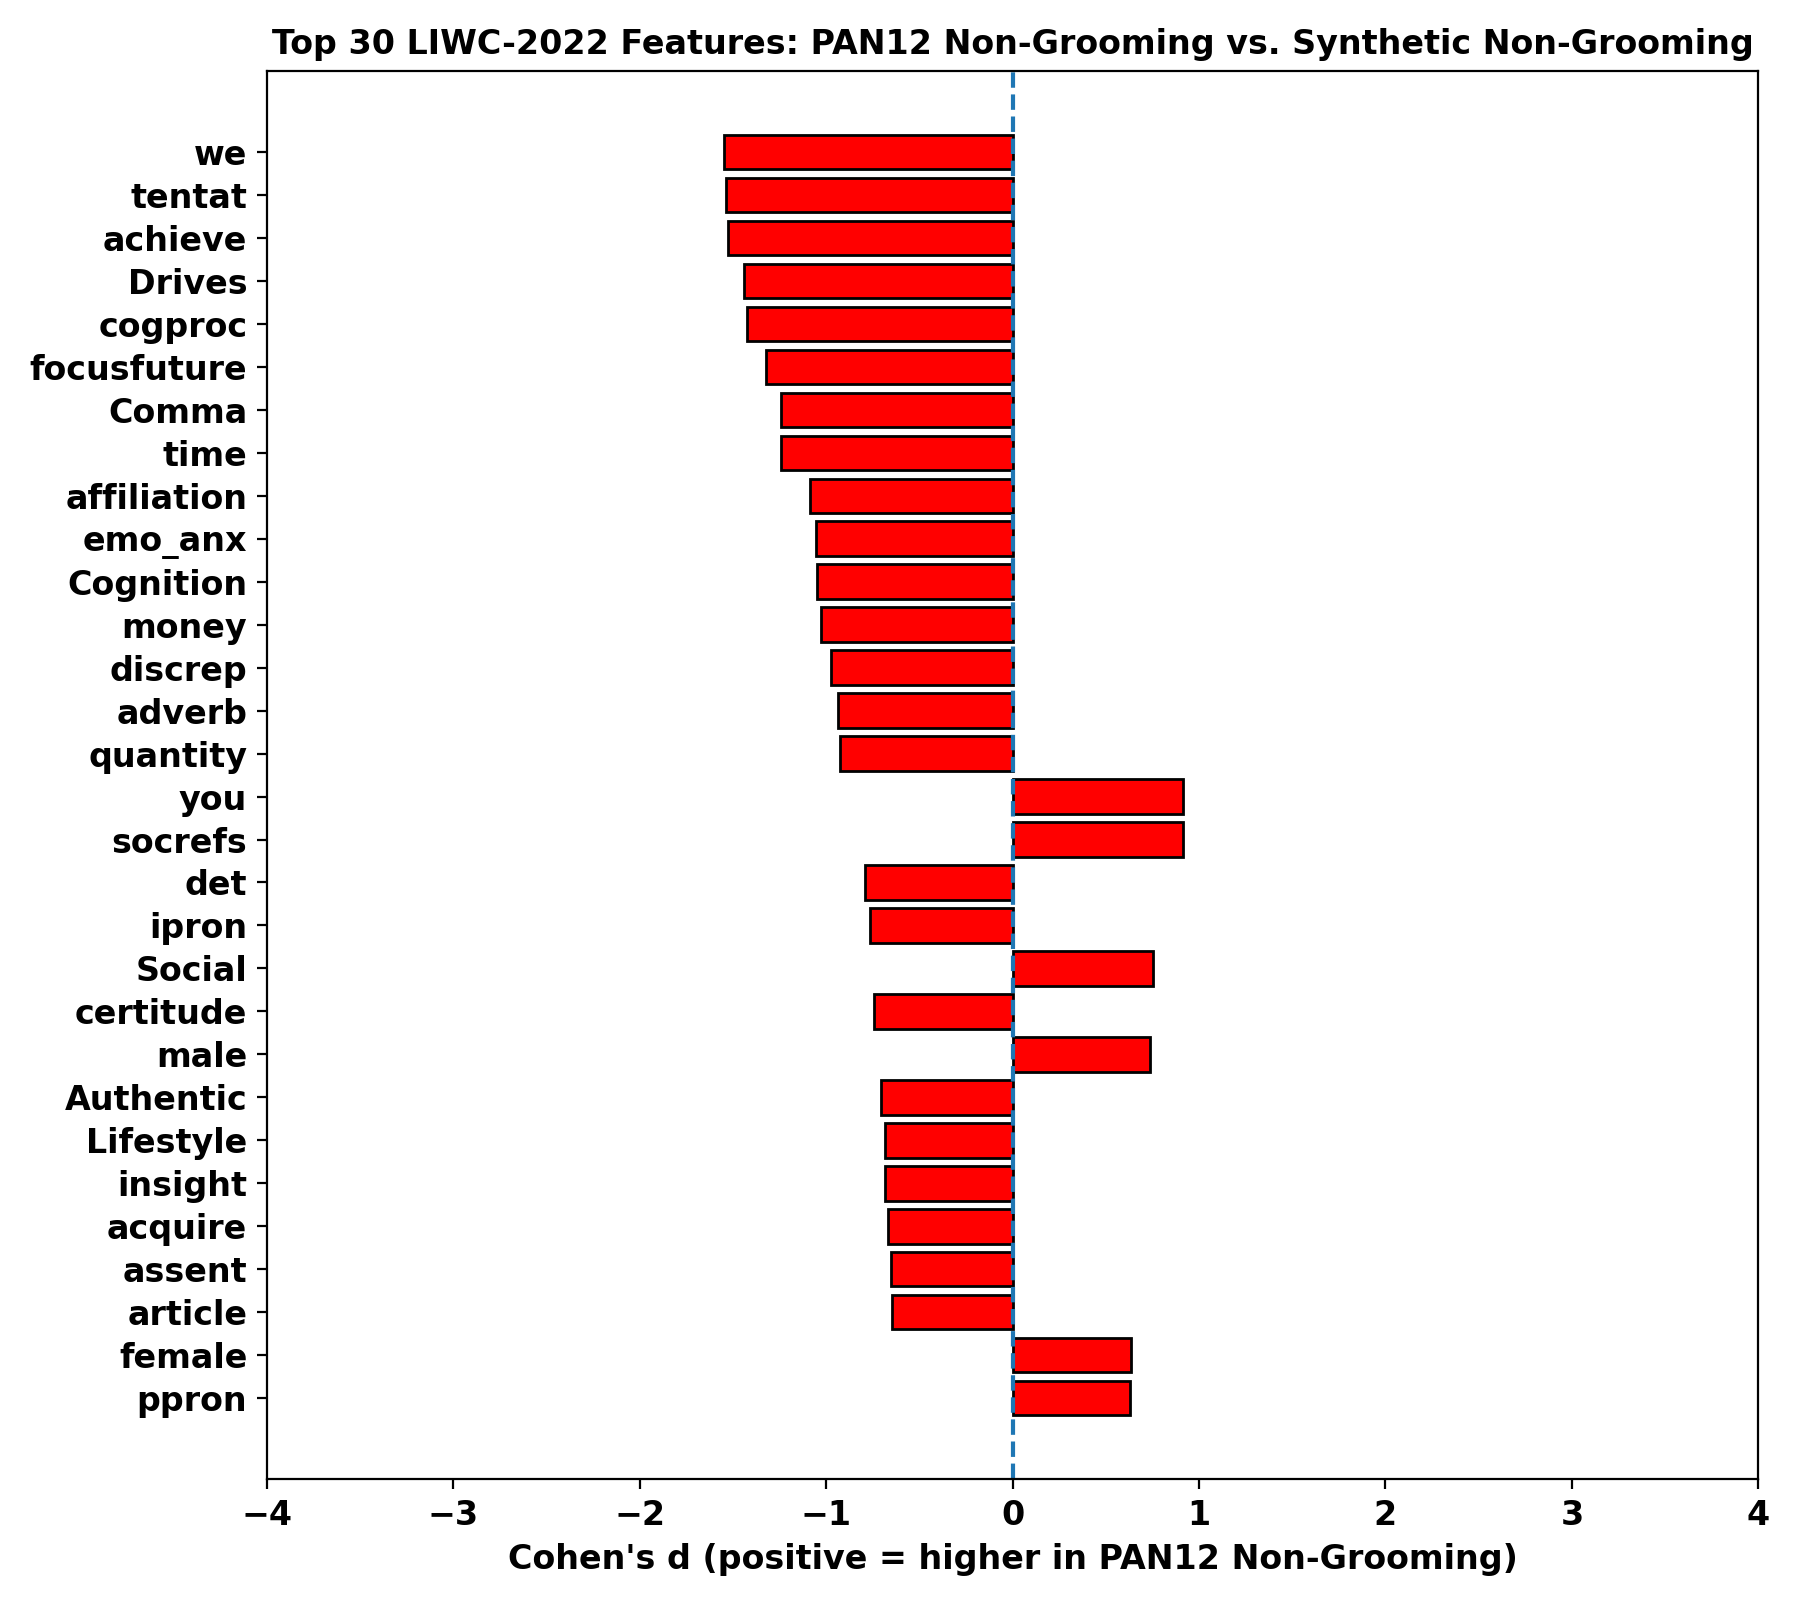
\includegraphics[width=\linewidth]{synthetic_comparison_pan.png}
    \caption{PAN12 vs. synthetic}
  \end{subfigure}
  \caption[Top 30 LIWC Differences with Synthetic Baseline]{Top LIWC differences with synthetic baseline based on cohens $d$ \cite{cohen1988}.}
  \label{fig:liwc_synth_side_by_side}
\end{figure}



Additionally, Figure~\ref{fig:liwc_synth_side_by_side} (left) shows the comparison between PJ and synthetic non-grooming data. Large discrepancies are visible across several LIWC dimensions, including strong positive shifts for all LIWC-categories such as \textit{Big Words}, \textit{ppron} and \textit{you}, suggesting that the synthetic samples over-represent certain linguistic markers.  Figure~\ref{fig:liwc_synth_side_by_side} (right) shows the comparison between PAN12 and the synthetic data. Here, the synthetic data again diverges notably across all LIWC-Categories. This confirms that the synthetic data differs clearly from both real corpora. Including such data in training therefore \textbf{challenges the model to generalize beyond the specific statistical patterns of PJ and PAN12 alone.}While this reduces predictive performance on real data in isolation only marginally, it improves the model’s ability to handle out-of-distribution examples, making the overall model more robust. Still, when interpreting the LIWC features of the predicted grooming and non-grooming class a clear distinction between real and synthetic data should be done, since the synthetic data postpones the real distribution in many LIWC-Categories.


\section{Chunk-based LIWC Analysis} \label{sec:chunk_based_liwc_analysis}


%%%% Überarbeitet

\begin{figure}[ht]
    \centering
    \begin{subfigure}[t]{0.49\textwidth}
        \centering
        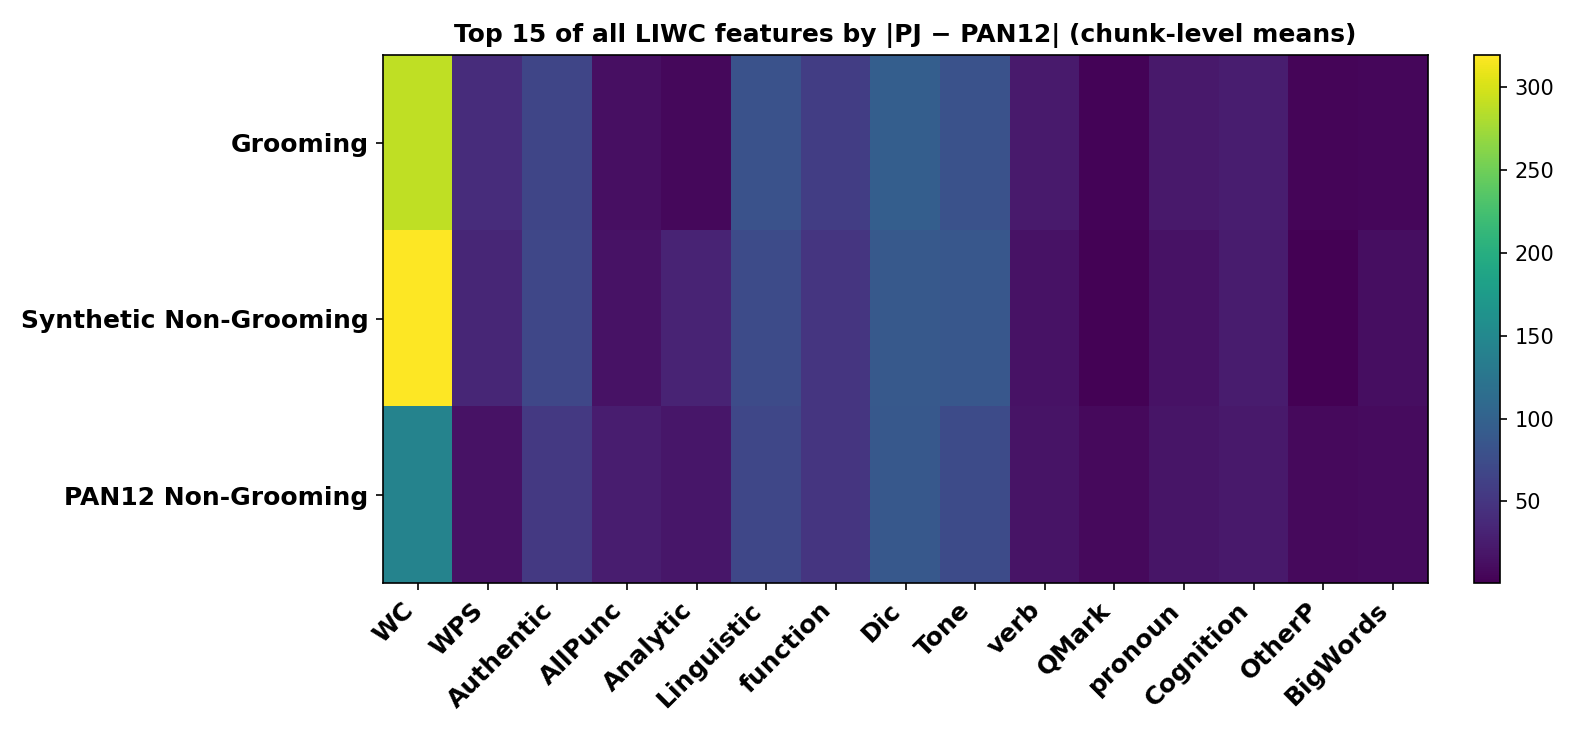
\includegraphics[width=\linewidth]{heatmap_topdiff_gobal.png}
        \caption{Top 15 LIWC categories on 512 chunk-level across all LIWC-2022 features.}
    \end{subfigure}
    \hfill
    \begin{subfigure}[t]{0.49\textwidth}
        \centering
        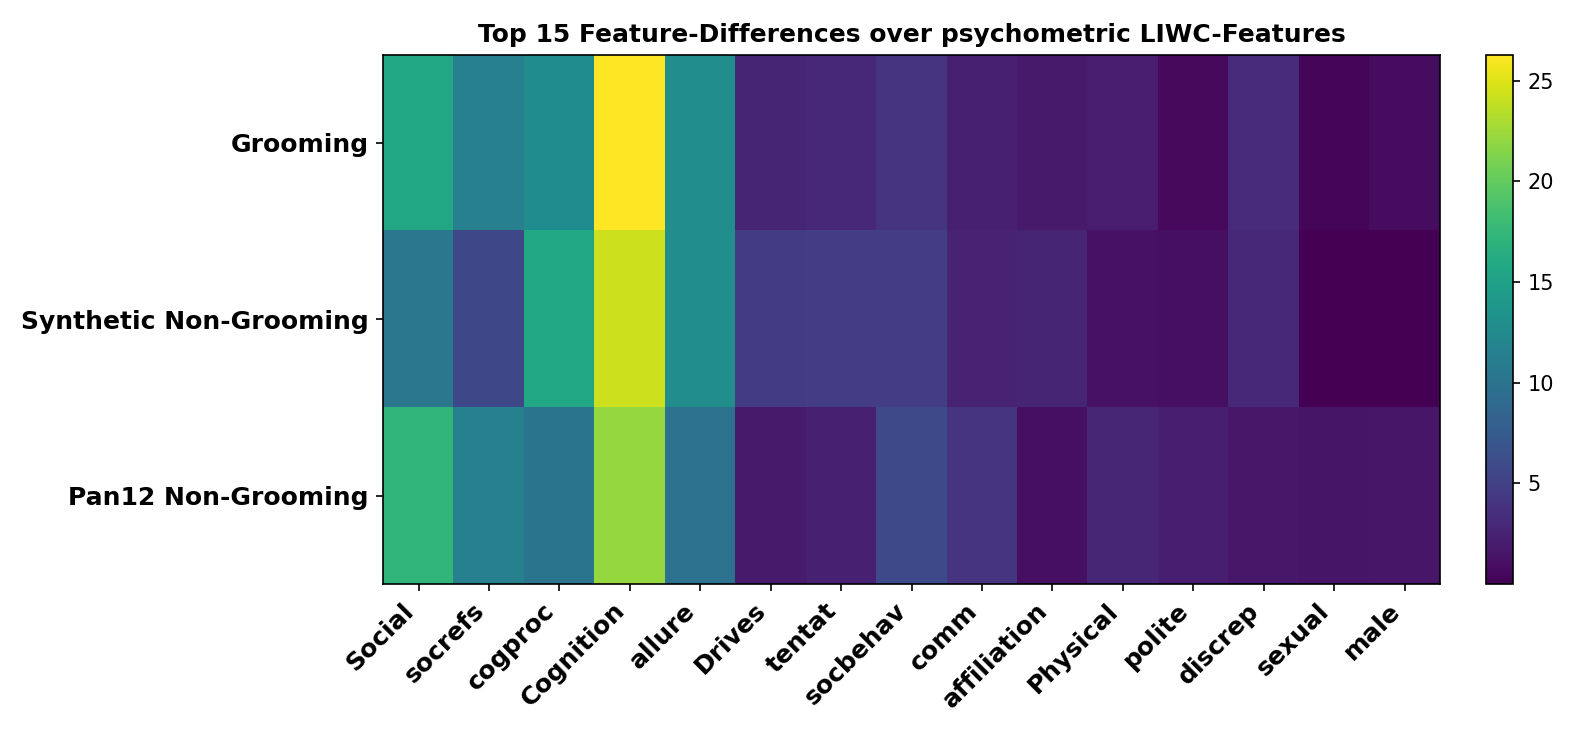
\includegraphics[width=\linewidth]{heatmap_topdiff_psycho.png}
        \caption{Top 15 LIWC-2022 features on 512 chunk-level highlighted in the literature.}
    \end{subfigure}
    \caption[LIWC Feature Comparison at Chunk Level]{LIWC feature comparison between grooming and non-grooming dialogues based on LIWC-2022 Features at chunk level.}
    \label{fig:liwc_chunked_analysis}
\end{figure}

In addition to an analysis of the overall conversations, an analysis of the LIWC features at the chunk level of 512 chunks (as used in the later feature fusion) was performed to analyze local variations across chats. 

Figure \ref{fig:liwc_chunked_analysis} shows a heat map of the top 30 mean features of grooming and non-grooming conversations (left) with the largest difference across all LIWC features and (right) with the largest difference across only the psychometric features highlighted in the literature. Rows represent PJ Grooming, Synthetic Non-Grooming and PAN12 Non-Grooming, while columns represent LIWC features. Color intensity encodes the mean feature value per source. The heatmaps show, that the LIWC features differ significantly througout all features and three sources at the chunk level, making it easier to understand how a model can already achieve high performance at this level.

When looking at the full feature set (left), it is noticeable, that the main differences between grooming and (synthetic) non-grooming chunks mainly lie on linguistic features such as \textit{word count}, \textit{WPS}, \textit{function words} and \textit{pronouns}, which are all more prevalent in grooming chunks. This confirms the earlier observation that grooming conversations tend to be longer and more linguistically rich, even at the chunk level. It can be seen, that the synthetic data have a very high word count balance out possible length leakage effects on chunk level. The differences in all other categories are less pronounced, but still visible with the real data seeming to be more similar across all LIWC-Categories than the synthetic data. 

When focusing on the psychometric features (right), the differences between grooming and non-grooming chunks become more pronounced. This could be due to the fact, that the scale of the psychometric features is smaller, making differences more visible since there is no feature like word count dominating the scale. It is noticeable, that grooming chunks show a values in features like \textit{Cogntition}, \textit{cognitive processes} and \textit{Allure} which could be caused by a content related reference to seduction and manipulation. Therefore grooming conversations are clearly distinguishable based on psychological strategies like building closeness (social/affilation), attraction (allure) and cognitive engagement (cognitive processes). It is striking that at the chunk level, the grooming conversations have a higher proportion of sexual words, which can be explained by the higher overall relations of sexual terms in smaller conversation segments. Still, the difference is not as strong as expected from prior work \cite{broome2020psycholinguistic,an2025cybergrooming}, which could be due to the fact that the PAN12 dataset contains a considerable amount of sexually explicit but non-grooming conversations. When comparing the synthetic non-grooming data to the real non-grooming data, it can be seen, that the synthetic data again shows a very different pattern across all psychometric features, confirming that the synthetic data differs clearly from both real corpora. 

This chunk-level perspective complements the global analysis by showing that distinguishing features are not only visible when analyzing entire conversations, but also occur within short text chunks. While the bar charts of the global analysis in Figure \ref{fig:liwc_global_analysis} highlight markers such as word count, pronoun usage and function words, the heat maps show that even locally, grooming dialogues have higher values in many categories. In particular, the dominance of sexual terms becomes apparent at the chunk level, as shorter segments amplify their relative frequency, whereas these signals are diluted in complete conversations due to more diverse linguistic content. At the same time, psychometric dimensions such as cognitive and social processes remain dominant in both analyses, underscoring their theoretical relevance.

Taken together, these results suggest that grooming behavior can be detected in the dataset through both global stylistic patterns and local lexical cues, which explains why BERT already shows very strong performance at the finetuning at chunk level.


\section{Feature Fusion Evaluation}

\begin{table}[H]
\centering
\small
\caption[Evaluation: Feature Fusion with all LIWC-2022 Features]{\textbf{Evaluation: Feature Fusion with all LIWC-2022 Features}}
\label{tab:fusion_all}
\begin{tabular}{@{}lrrrrr@{}} % <-- 6 Spalten (l + 5x r)
\toprule
& \multicolumn{5}{c}{\textbf{Test Set Metrics}} \\
\cmidrule(lr){2-6}
\textbf{Step (Epoch)} & \textbf{Loss} & \textbf{Accuracy} & \textbf{Precision} & \textbf{Recall} & \textbf{F1} \\
\midrule
3000 (0.76)  & 0.234 & 0.985 & 0.959 & 0.989 & \textbf{0.974} \\
6000 (1.52)  & 0.231 & 0.987 & 0.962 & 0.994 & \textbf{0.978} \\
9000 (2.28)  & 0.218 & 0.993 & 0.983 & 0.992 & \textbf{0.987} \\
11865 (3.00) & 0.218 & 0.993 & 0.989 & 0.985 & \textbf{0.987} \\
\bottomrule
\end{tabular}
\end{table}


\begin{table}[H]
\centering
\caption[Evaluation: Feature Fusion with LIWC-2022 Subset]{\textbf{Evaluation: Feature Fusion with Subset of LIWC-2022 Features}}
\small
\label{tab:fusion_subset}
\begin{tabular}{@{}lrrrrr@{}} % <-- 6 Spalten
\toprule
& \multicolumn{5}{c}{\textbf{Test Set Metrics}} \\
\cmidrule(lr){2-6}
\textbf{Step (Epoch)} & \textbf{Loss} & \textbf{Accuracy} & \textbf{Precision} & \textbf{Recall} & \textbf{F1} \\
\midrule
3000 (0.76)  & 0.249 & 0.976 & 0.925 & 0.996 & \textbf{0.959} \\
6000 (1.52)  & 0.221 & 0.991 & 0.983 & 0.985 & \textbf{0.984} \\
9000 (2.28)  & 0.219 & 0.992 & 0.990 & 0.983 & \textbf{0.986} \\
11865 (3.00) & 0.218 & 0.993 & 0.989 & 0.986 & \textbf{0.987} \\
\bottomrule
\end{tabular}
\end{table}

The presented tables \ref{tab:fusion_all} and \ref{tab:fusion_subset} summarize the performance of the feature fusion model that combines BERT embeddings with LIWC-2022 features. Both configurations were evaluated at four training steps (3000, 6000, 9000 and 11865), corresponding to epochs of 0.76, 1.52, 2.28 and 3.00.

\subsection{Using all LIWC-2022 Features}

When using all LIWC-2022 features (Table \ref{tab:fusion_all}), the fusion model achieved an improvement of the F1 score in all training steps of the feature-fusion model, starting from 0.974 at 3000 steps and reaching up to 0.987 at 11865 steps. This indicates that the additional psycholinguistic information provided by the LIWC features helps the model better distinguish between grooming and non-grooming conversations. It is striking, that the precision increased in all training steps from 0.935 to 0.959 at 3000 steps and up to a total difference of 4.4 \% to 0.989 at 11865 steps. This suggests that the fusion model is more effective at reducing false positives, which is crucial in practical applications where misclassifying non-grooming conversations as grooming can have serious consequences. On the other hand, there was a small decrease in recall from 0.990 to 0.989 at 3000 steps and from 0.996 to 0.985 at 11865 steps, indicating that the model is slightly less sensitive in identifying all grooming cases. This leads to the conclusion, that the fusion model is more conservative in its predictions using additional LIWC features, which may be beneficial in reducing false alarms while still maintaining high overall accuracy.


\subsection{Using a Subset of Psychometric LIWC-2022 Features}

When using only a subset of psychometric LIWC-2022 features (table \ref{tab:fusion_subset}), the same trend of improvement in F1 score was observed, starting from 0.959 at 3000 steps and reaching up to 0.987 at 11865 steps. This indicates that even a targeted selection of psycholinguistically relevant features can significantly enhance model performance. The precision also showed a substantial increase from 0.925 to 0.959 at 3000 steps and up to 0.989 at 11865 steps, similar to the results when using all features. This reinforces the idea that psychometric features are particularly valuable in improving the model's ability to correctly identify grooming conversations while minimizing false positives. However, the recall showed a slight decrease from 0.996 to 0.985 at 6000 steps and from 0.983 to 0.986 at 11865 steps, indicating a minor trade-off in sensitivity. Overall, the results suggest that even a focused set of psychometric LIWC features can provide benefits when fused with BERT embeddings, enhancing the model's robustness and reliability in detecting grooming behavior.


\subsection{Confusion Matrices for Feature Fusion Models}


\begin{figure}[H]
  \centering

  % -------- Top row: Feature fusion with ALL LIWC-2022 features --------
  \begin{subfigure}[t]{0.32\textwidth}
    \centering
    % \includegraphics[width=\linewidth,trim={0 10 0 28},clip]{fusion_all_epoch01_confmat.png}
    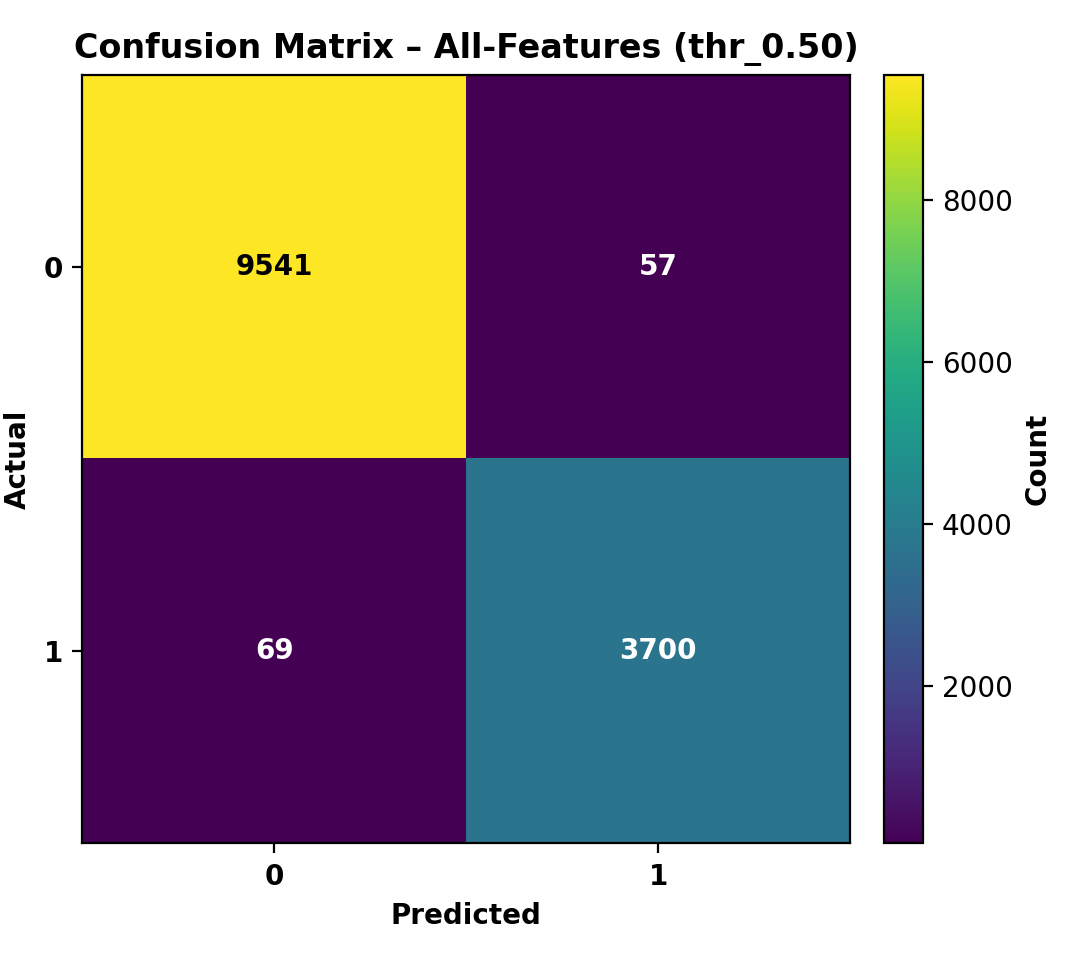
\includegraphics[width=\linewidth]{plots_feature_fusion_all/fusion_eval_epoch_1/confusion_matrix_all_thr_0.50.png}
    \caption{Epoch 1}
    \label{fig:ff_all_e1}
  \end{subfigure}\hfill
  \begin{subfigure}[t]{0.32\textwidth}
    \centering
    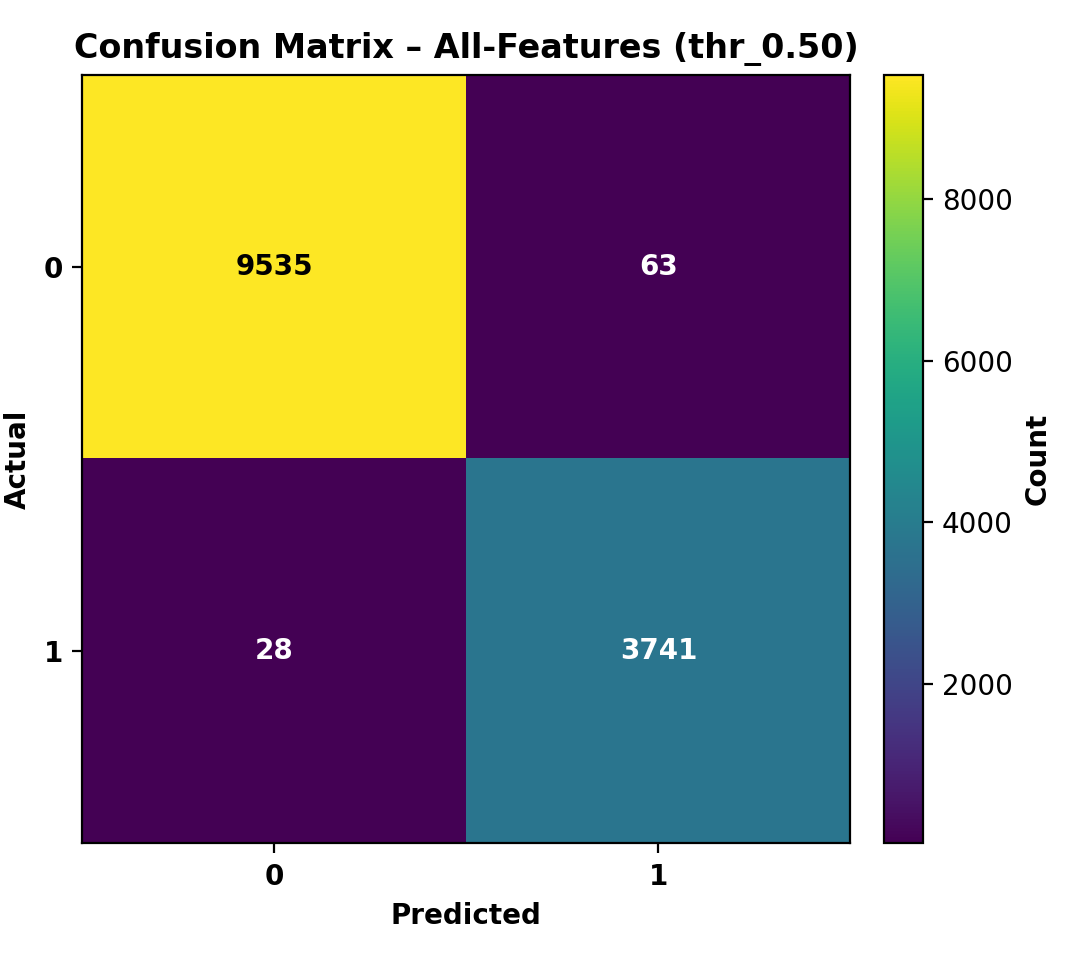
\includegraphics[width=\linewidth]{plots_feature_fusion_all/fusion_eval_epoch_2/confusion_matrix_all_thr_0.50.png}
    \caption{Epoch 2}
    \label{fig:ff_all_e2}
  \end{subfigure}\hfill
  \begin{subfigure}[t]{0.32\textwidth}
    \centering
    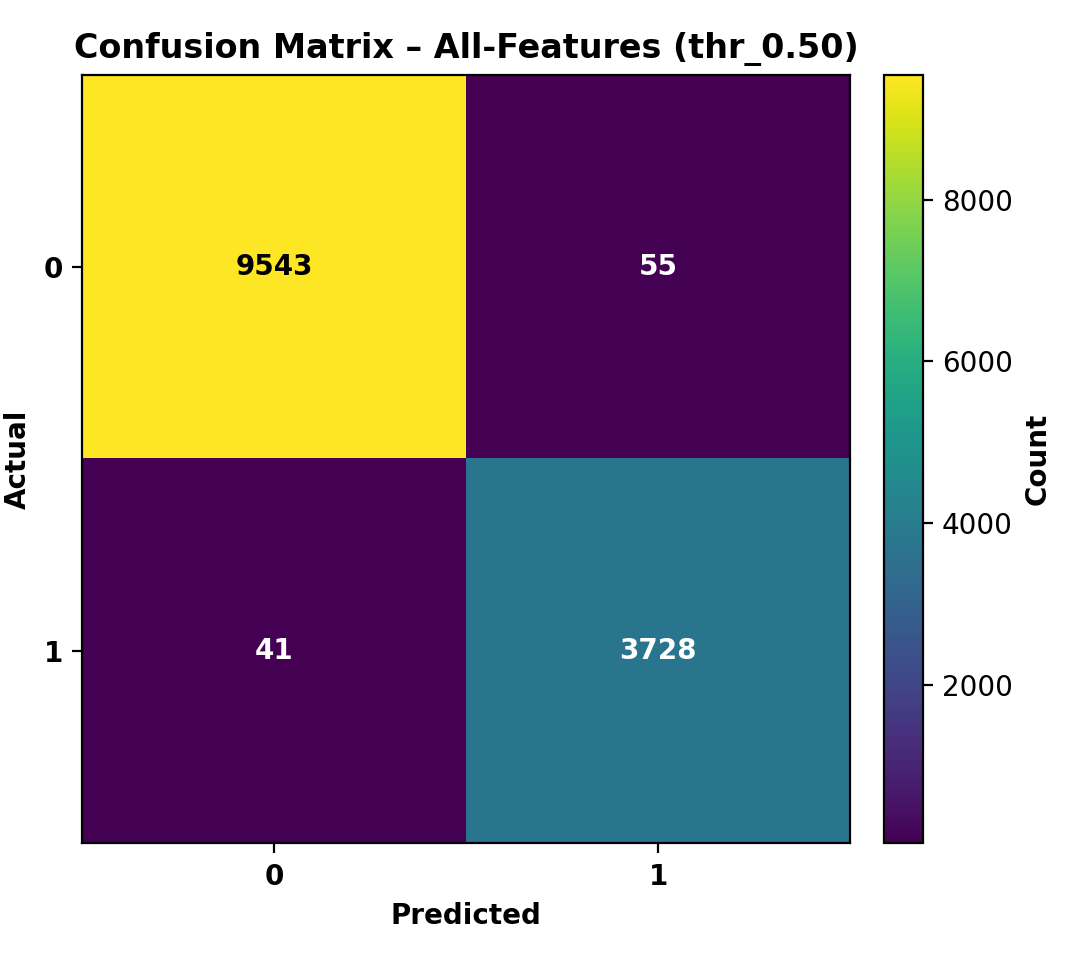
\includegraphics[width=\linewidth]{plots_feature_fusion_all/fusion_eval_epoch_3/confusion_matrix_all_thr_0.50.png}
    \caption{Epoch 3}
    \label{fig:ff_all_e3}
  \end{subfigure}

  \vspace{0.45cm}

  % -------- Bottom row: Feature fusion with PSYCHOMETRIC subset --------
  \begin{subfigure}[t]{0.32\textwidth}
    \centering
    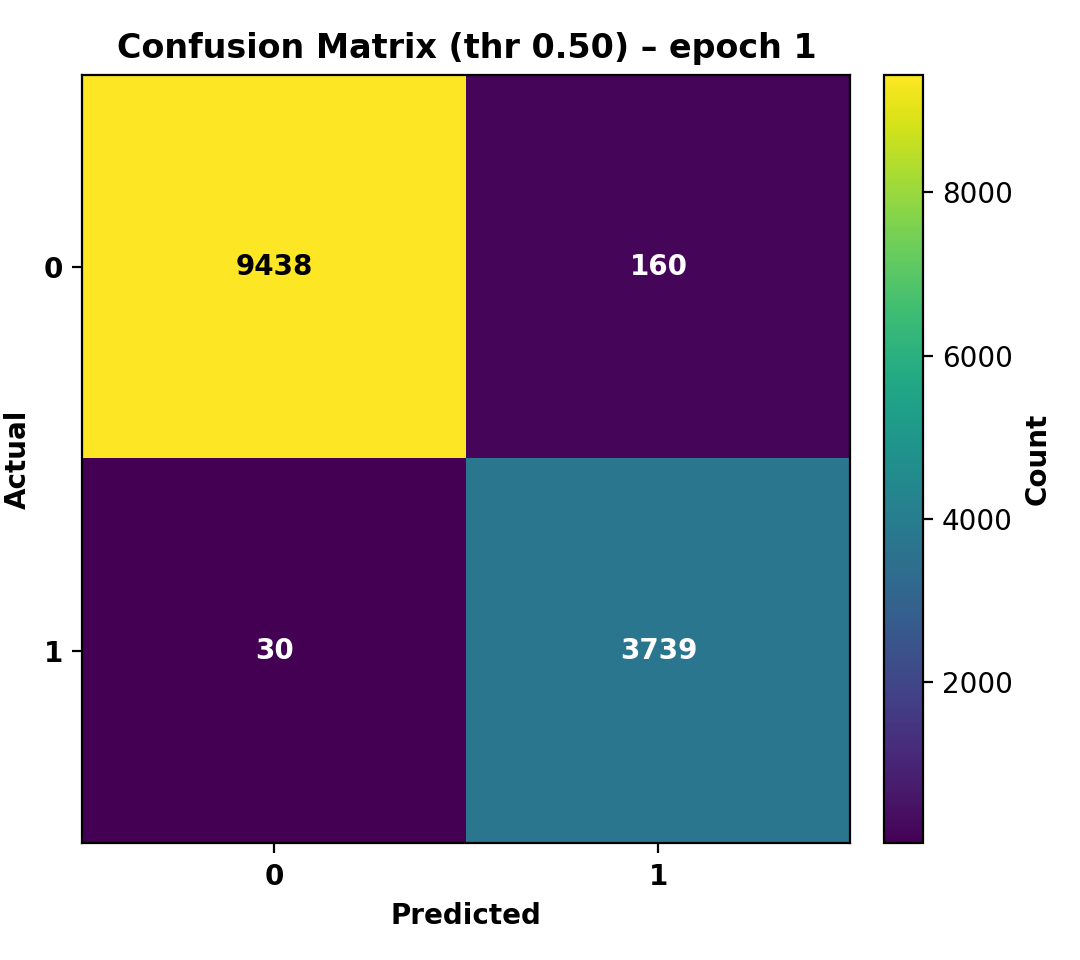
\includegraphics[width=\linewidth]{plots_feature_fusion_subset/epch_1_plots/confmat_thr_0.50_epoch_1.png}
    \caption{Epoch 1}
    \label{fig:ff_psy_e1}
  \end{subfigure}\hfill
  \begin{subfigure}[t]{0.32\textwidth}
    \centering
    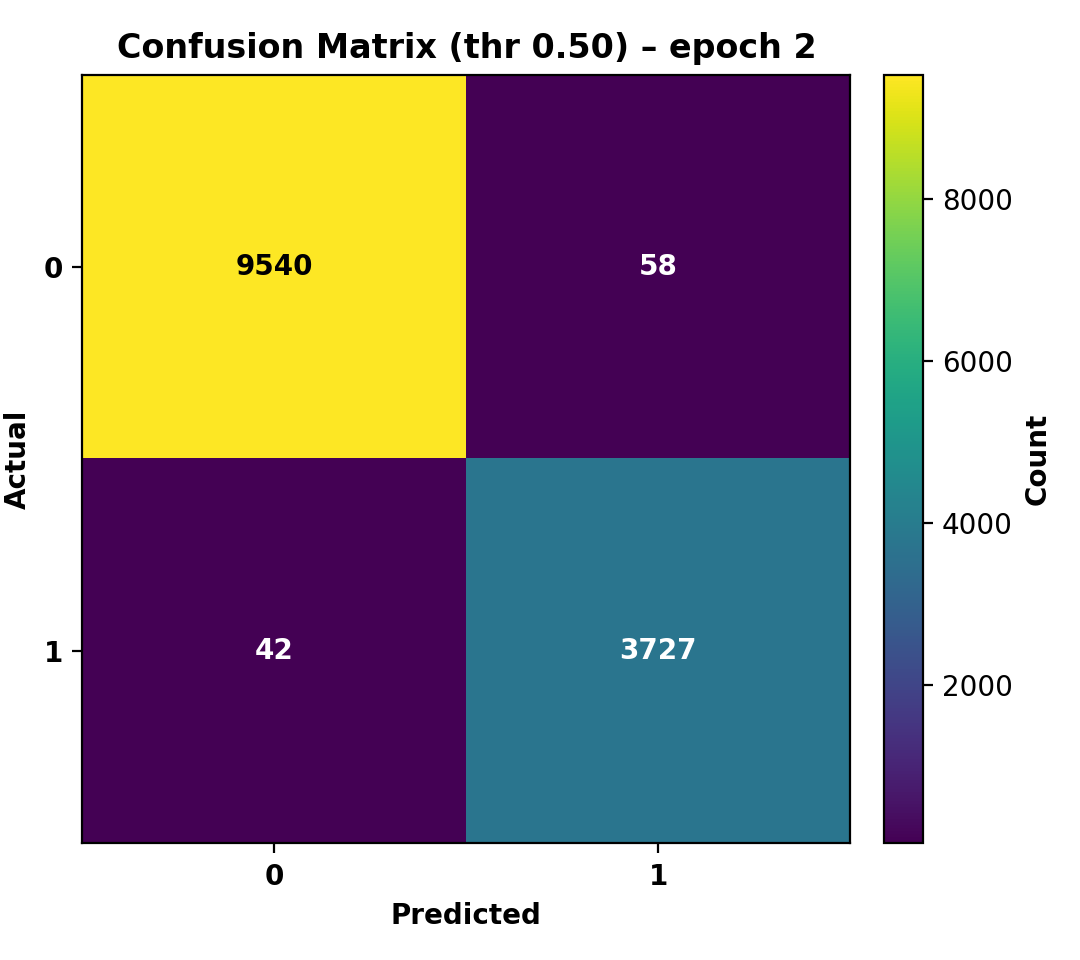
\includegraphics[width=\linewidth]{plots_feature_fusion_subset/epoch_2_plots/confmat_thr_0.50_epoch_2.png}
    \caption{Epoch 2}
    \label{fig:ff_psy_e2}
  \end{subfigure}\hfill
  \begin{subfigure}[t]{0.32\textwidth}
    \centering
    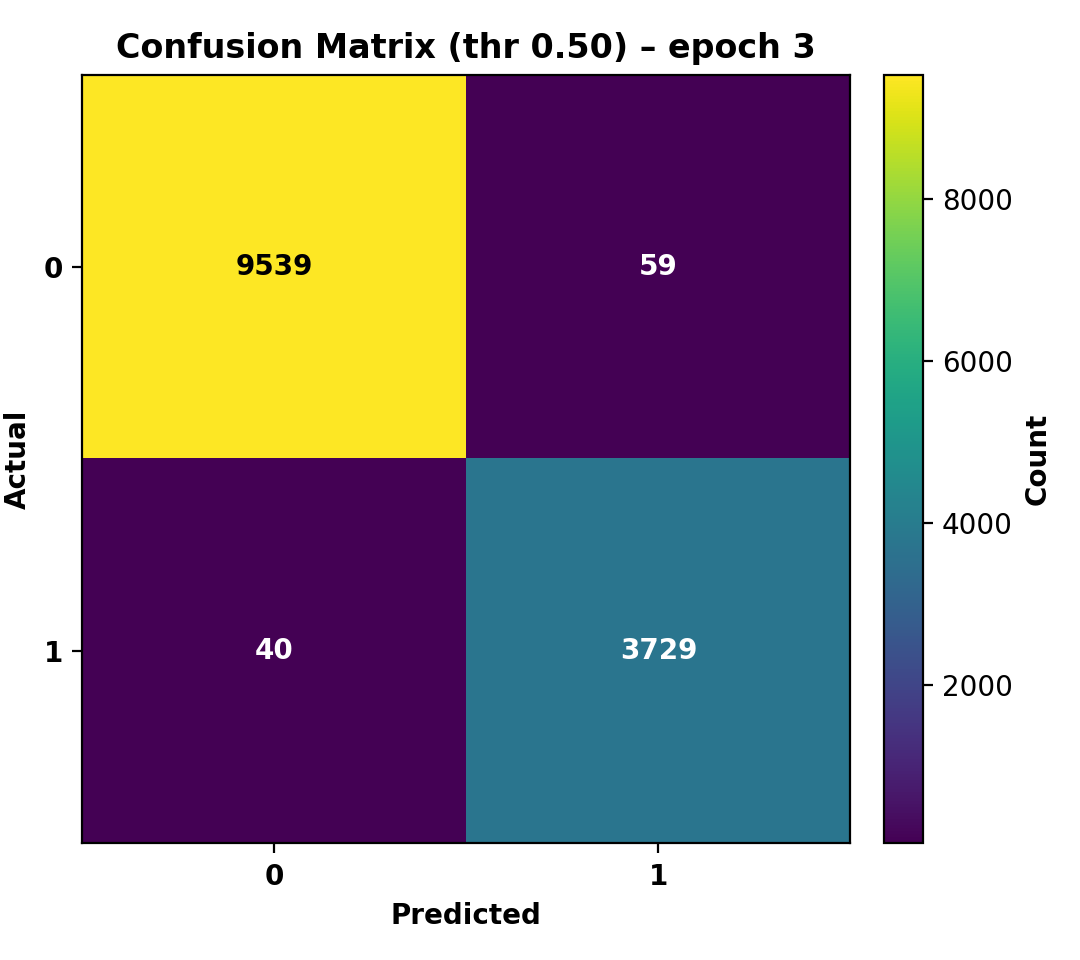
\includegraphics[width=\linewidth]{plots_feature_fusion_subset/epoch_3_plots/confmat_thr_0.50_epoch_3.png}
    \caption{Epoch 3}
    \label{fig:ff_psy_e3}
  \end{subfigure}

  \caption[Confusion matrices by epoch for feature-fusion models.]{\textbf{Confusion matrices by epoch for feature-fusion models (BERT baseline).}
  \emph{Top row:} fusion with all LIWC-2022 features. \emph{Bottom row:} fusion with the psychometric LIWC-2022 subset.
  Each panel shows true labels (rows) vs. predicted labels (columns); diagonal cells indicate correct predictions, off-diagonal cells are errors. The confusion matrices were generated using a classification threshold of 0.5.
  For fair visual comparison, keep the same color scale across all panels.}
  \label{fig:ff_confmats_epochs}
\end{figure}

Figure \ref{fig:ff_confmats_epochs} shows the confusion matrices for both feature-fusion configurations across three epochs. It is notable that both configurations achieve a very balanced performance, having very high true positive rates (TPR) and true negative rates (TNR), with stable values across all epochs, indicating excellent overall classification performance. The number of false positives (FP) and false negatives (FN) is very low in all cases, demonstrating that the models are effective at minimizing both types of errors. 

When comparing the two configurations, it is evident that the model using all LIWC-2022 features shows a slightly better performance in epoch 1, with fewer false positives and false negatives compared to the model using only the psychometric subset. However, as training progresses to epochs 2 and 3, the differences between the two configurations become negligible, with both achieving nearly identical performance in epoch 3. This suggests that while the additional LIWC features may provide some initial benefit, the psychometric subset is sufficient for achieving high accuracy once the model has been adequately trained. Consequently, the confusion matrices reveal that both models maintain high sensitivity and specificity across all three epochs of training and for both configurations (all LIWC features and only psychometric subset of features). This suggests that the feature-fusion approach effectively balances the trade-off between detecting grooming conversations and avoiding false alarms. Also, when comparing the feature fusion models to the BERT-Baseline with 512 Chunks and a mixed split \ref{fig:bert_confusionmatrices_epoch3}, it is evident, that the feature fusion models achieve a smaller false positive rate, indicating a more "conservative" classification behavior, which is particularly important in practical applications where false alarms can have serious consequences. However, as already shown in table \ref{tab:fusion_all} and \ref{tab:fusion_subset}, there is a small increase in the false positive rate, indicating a minor trade-off in sensitivity. Still, the differences are relatively small, suggesting that while LIWC features provide additional value, the BERT embeddings already capture much of the relevant information. Overall, the results suggest that the feature-fusion approach is better in classifying non-grooming conversations directly but with a small increase in the false negative rate but an overall more balanced performance than the BERT baseline.


\subsection{ROC Curves for Feature Fusion Models}

%%%%%% ROC CURVES

\begin{figure}[H]
  \centering

  % -------- Top row: Feature fusion with ALL LIWC-2022 features --------

  % -------- Bottom row: Feature fusion with PSYCHOMETRIC subset --------
  \begin{subfigure}[t]{0.32\textwidth}
    \centering
    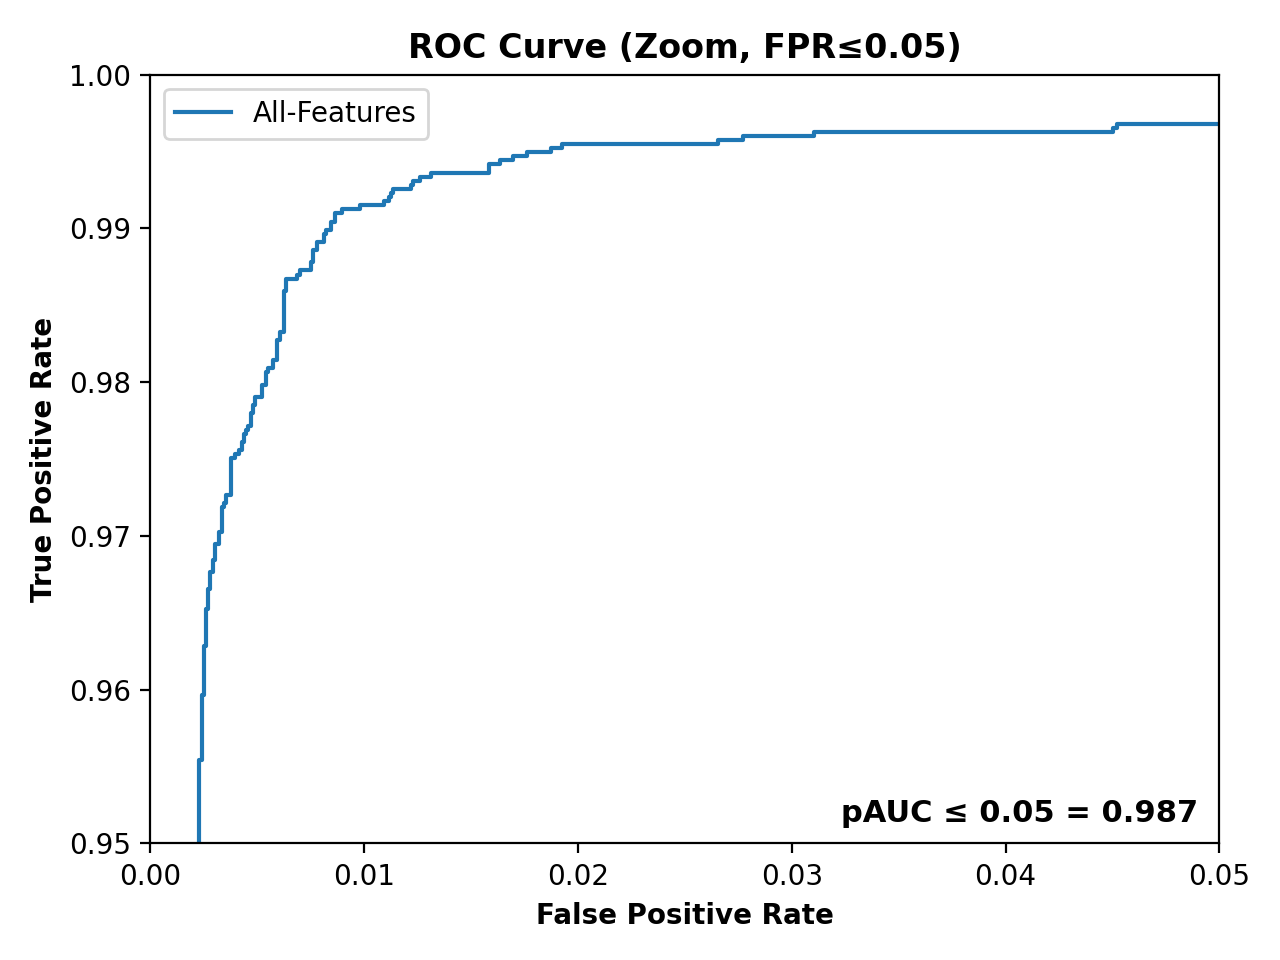
\includegraphics[width=\linewidth]{plots_feature_fusion_all/fusion_eval_epoch_1/roc_curve_all_zoom.png}
    \caption{Epoch 1}
    \label{fig:ffroc_psy_e1}
  \end{subfigure}\hfill
  \begin{subfigure}[t]{0.32\textwidth}
    \centering
    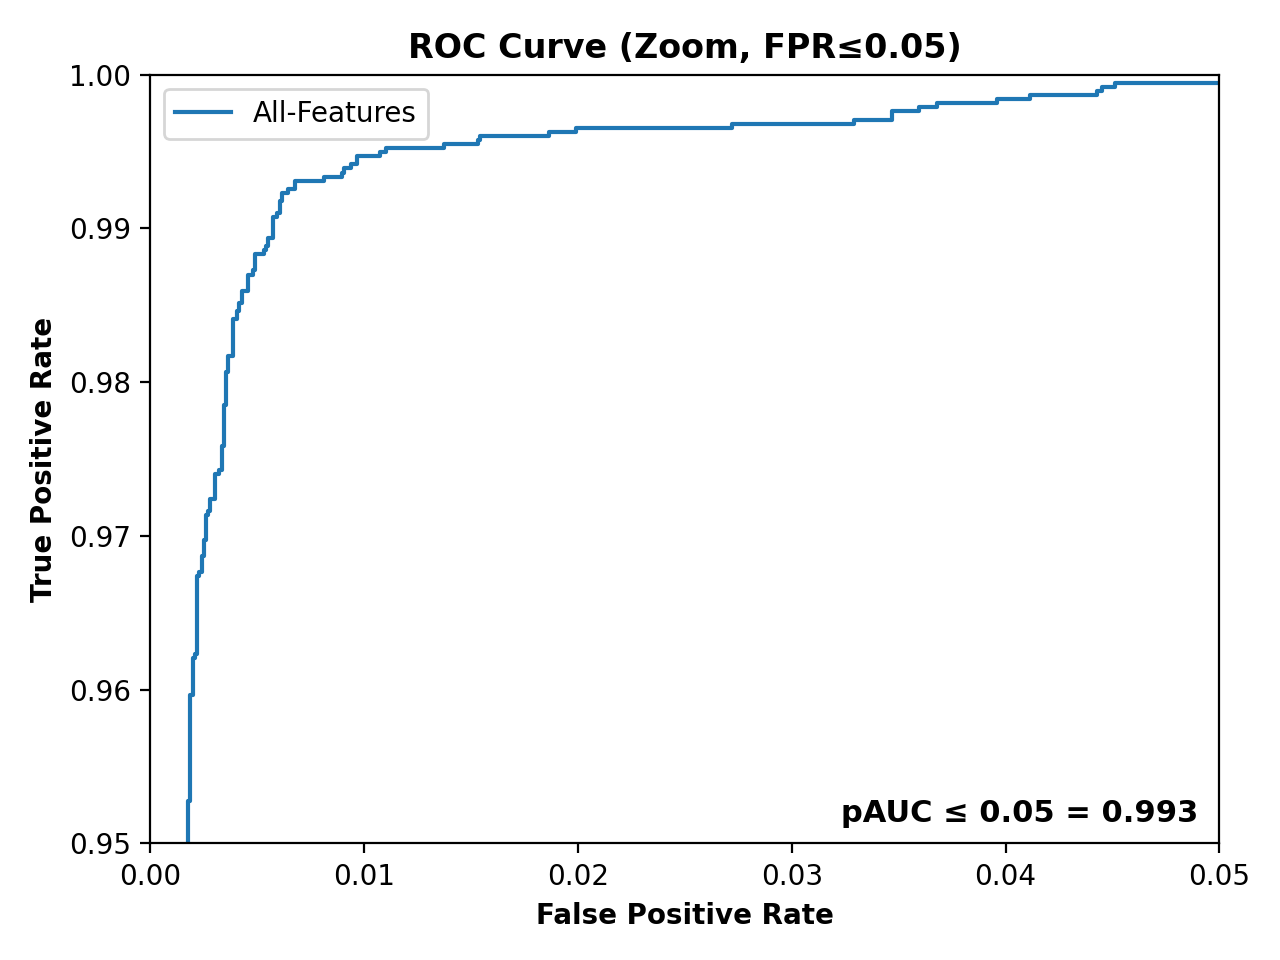
\includegraphics[width=\linewidth]{plots_feature_fusion_all/fusion_eval_epoch_2/roc_curve_all_zoom.png}
    \caption{Epoch 2}
    \label{fig:ffroc_psy_e2}
  \end{subfigure}\hfill
  \begin{subfigure}[t]{0.32\textwidth}
    \centering
    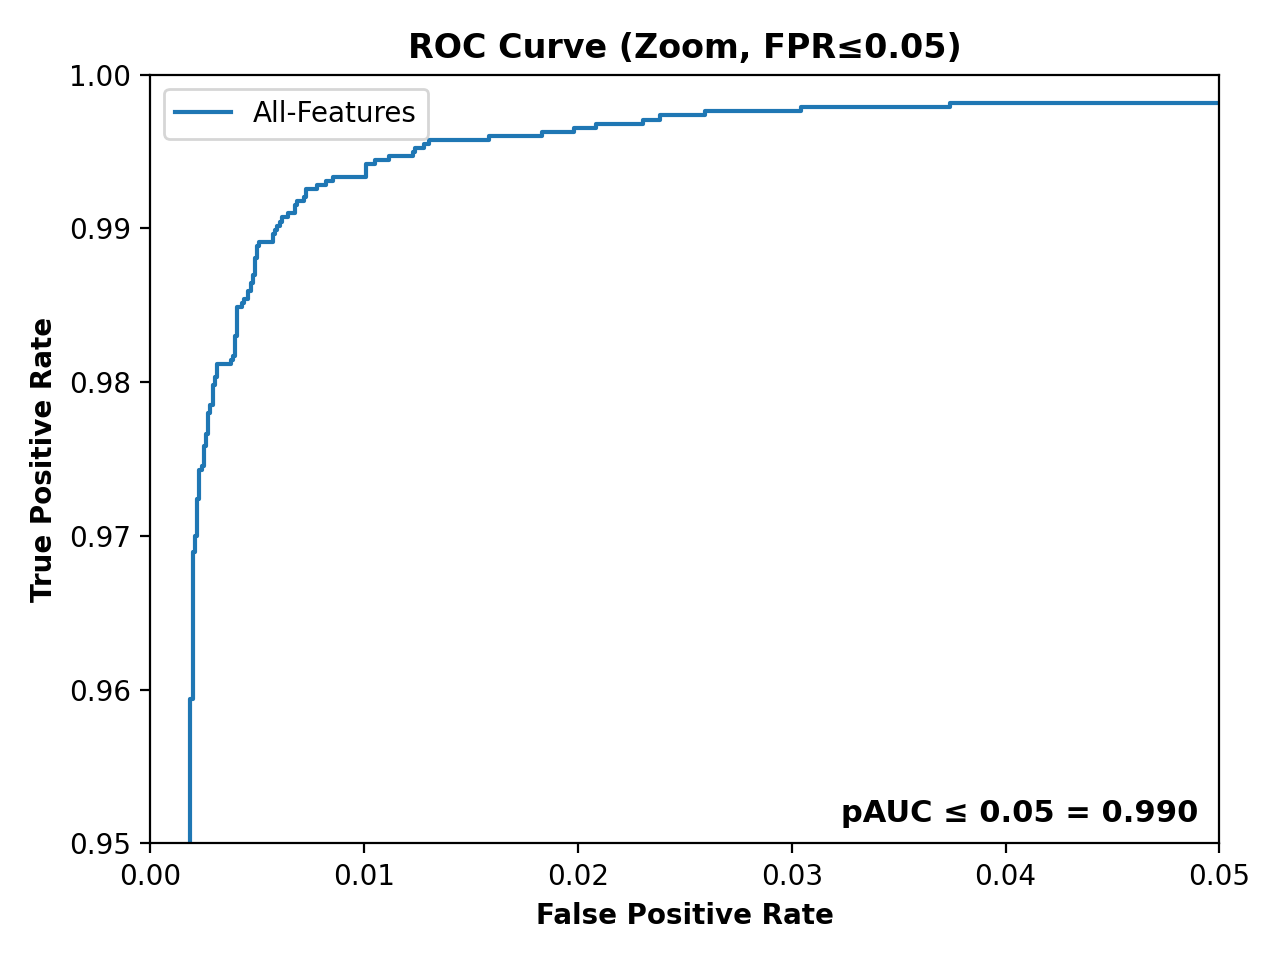
\includegraphics[width=\linewidth]{plots_feature_fusion_all/fusion_eval_epoch_3/roc_curve_all_zoom.png}
    \caption{Epoch 3}
    \label{fig:ffroc_psy_e3}
  \end{subfigure}

    \vspace{0.45cm}


    \begin{subfigure}[t]{0.32\textwidth}
    \centering
    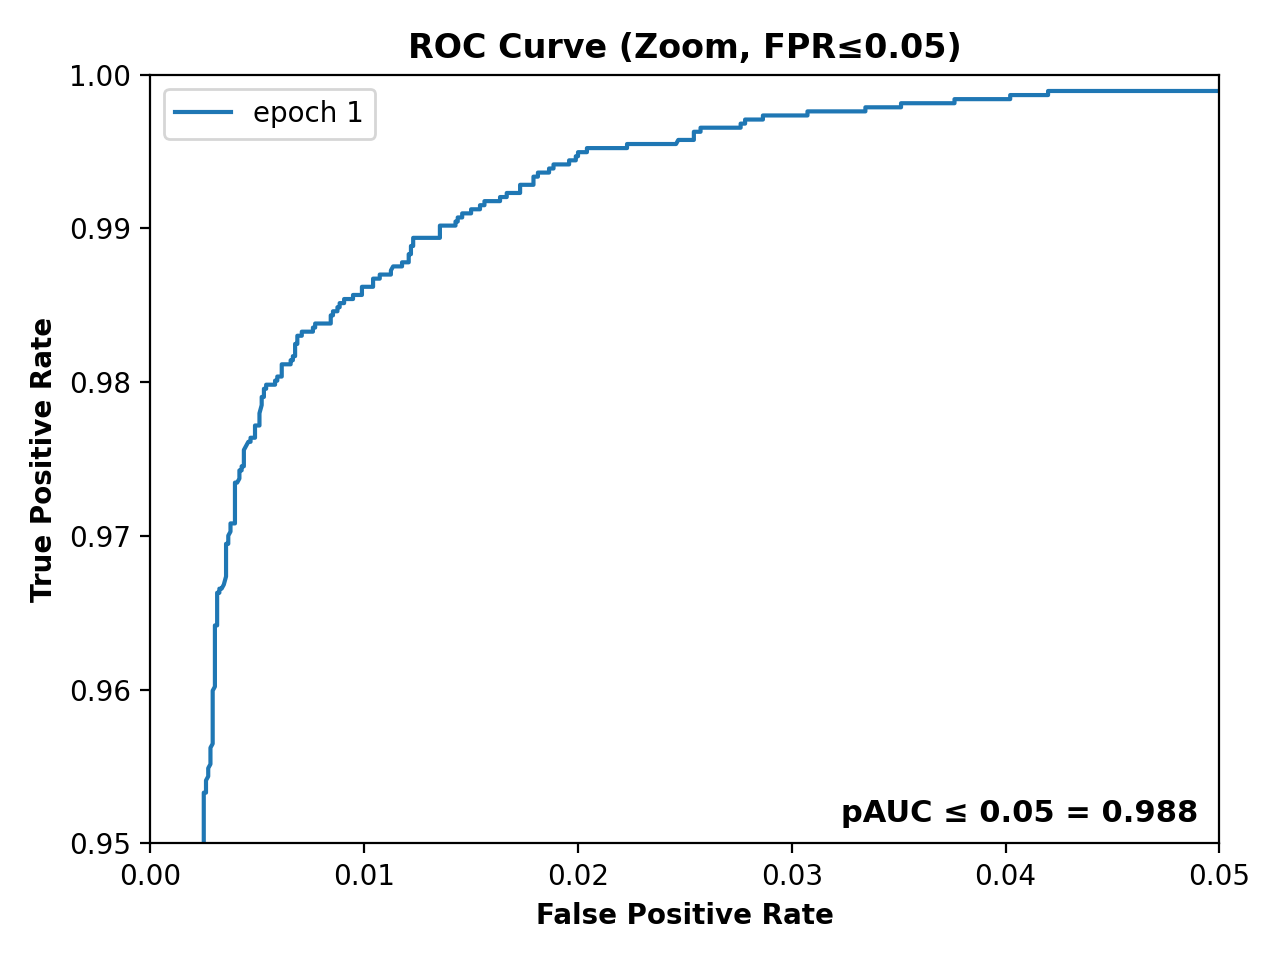
\includegraphics[width=\linewidth]{plots_feature_fusion_subset/epch_1_plots/roc_zoom_epoch_1.png}
    \caption{Epoch 1}
    \label{fig:ffroc_all_e1}
  \end{subfigure}\hfill
  \begin{subfigure}[t]{0.32\textwidth}
    \centering
    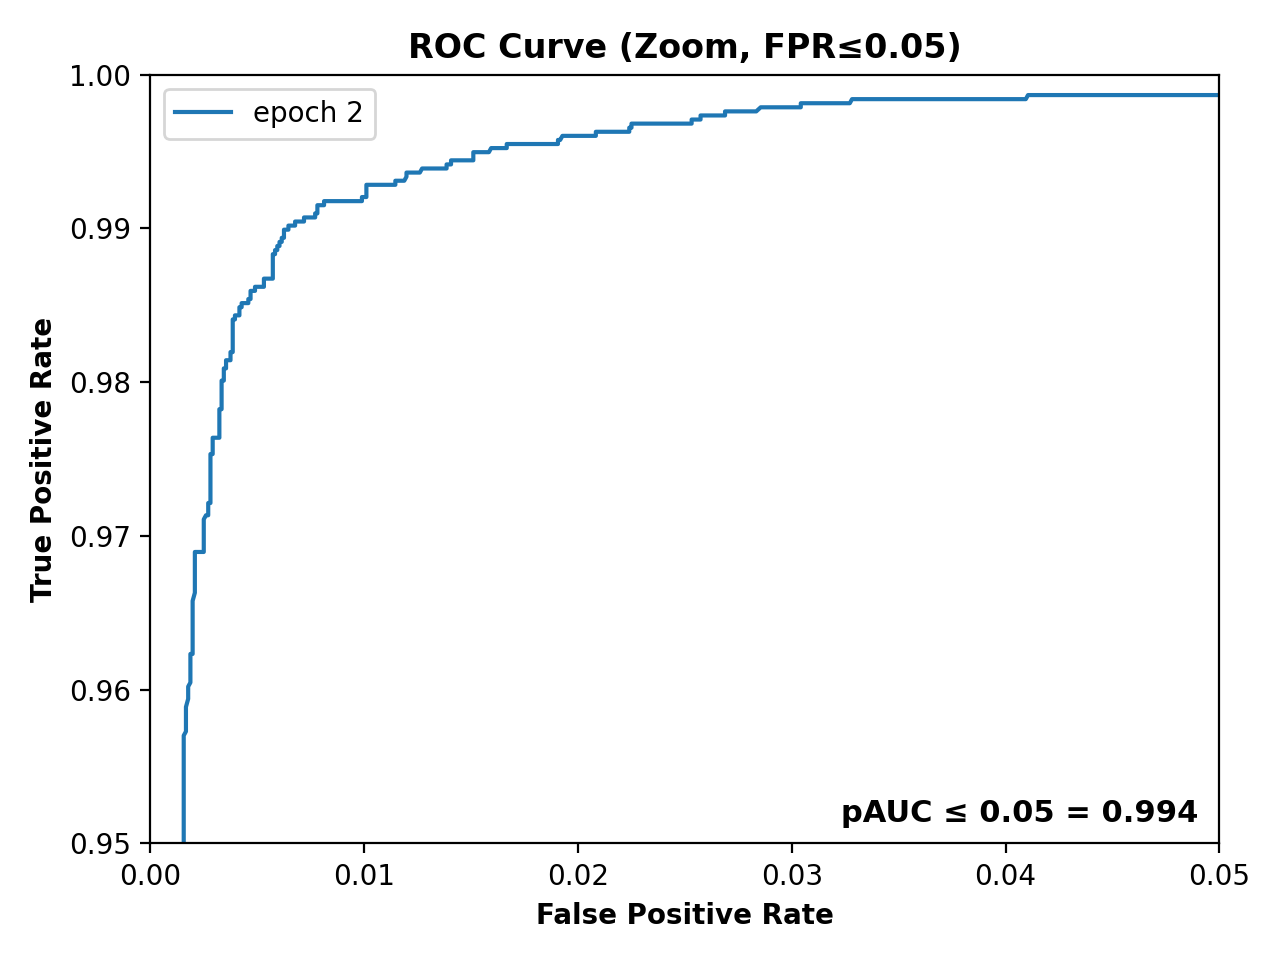
\includegraphics[width=\linewidth]{plots_feature_fusion_subset/epoch_2_plots/roc_zoom_epoch_2.png}
    \caption{Epoch 2}
    \label{fig:ffroc_all_e2}
  \end{subfigure}\hfill
  \begin{subfigure}[t]{0.32\textwidth}
    \centering
    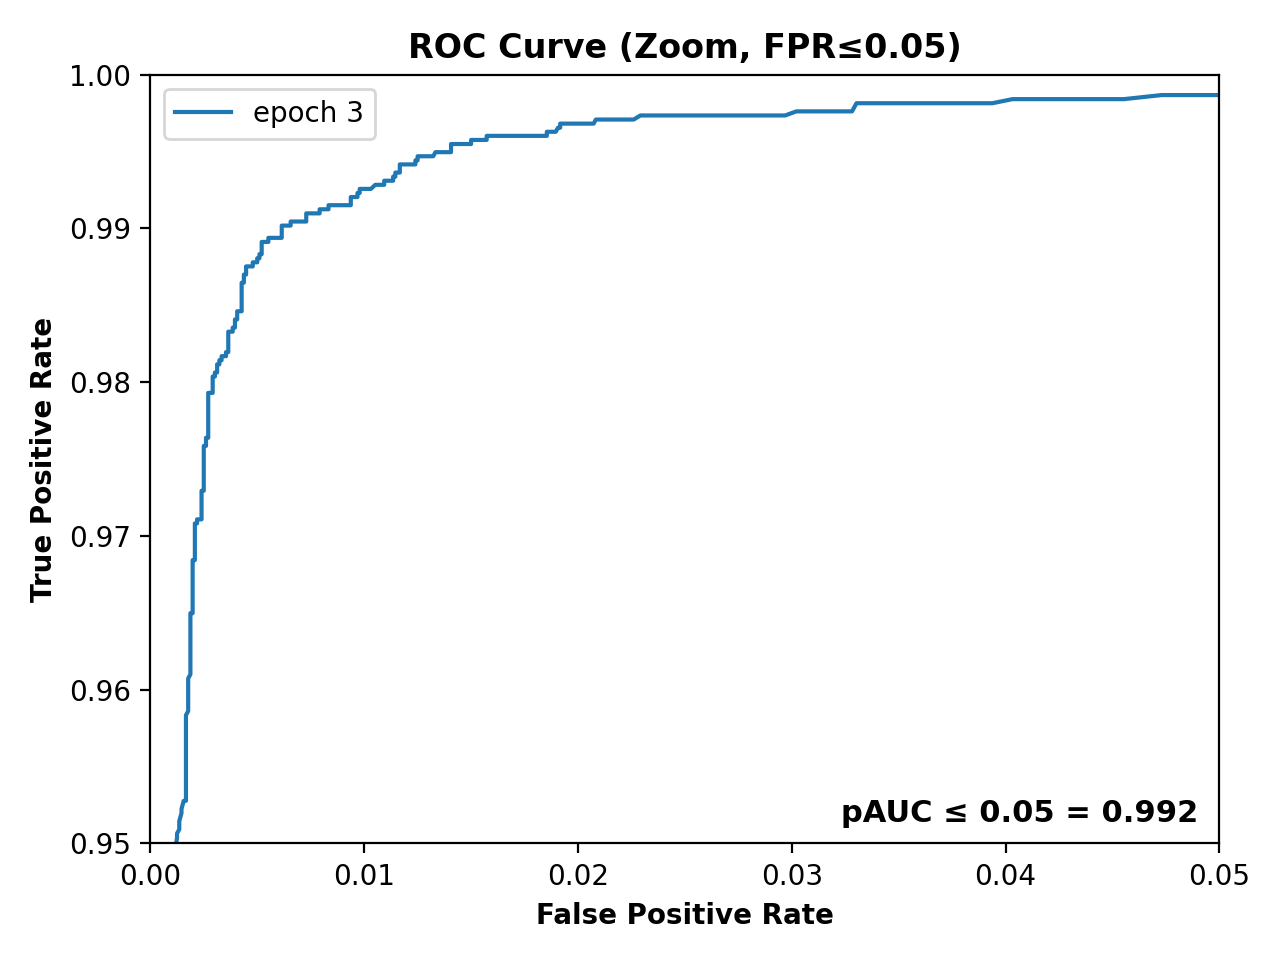
\includegraphics[width=\linewidth]{plots_feature_fusion_subset/epoch_3_plots/roc_zoom_epoch_3.png}
    \caption{Epoch 3}
    \label{fig:ffroc_all_e3}
  \end{subfigure}


  \caption[Zoomed ROC curves for feature-fusion models across epochs.]{\textbf{Zoomed ROC curves for feature-fusion models across all three epochs.}
  \emph{Top row:} fusion with all LIWC-2022 features. \emph{Bottom row:} fusion with the psychometric LIWC-2022 subset.
  Columns show epochs 1–3. All panels display the same zoom window to highlight differences at low false-positive rates
  (\(\mathrm{FPR}\le 0.05,\ \mathrm{TPR}\ge 0.95\)); the legend in each plot reports the pAUC of the \emph{full} ROC curve.}
  \label{fig:ff_roc_zoom_epochs}
\end{figure}

Figure \ref{fig:ff_roc_zoom_epochs} shows the zoomed ROC curves for both feature-fusion configurations across three epochs. It is notable that both configurations achieve very high pAUC values, indicating excellent overall discrimination between grooming and non-grooming conversations. Also, the curves for both configurations are very steep at a very low false positive rate, indicating that the models can achieve high true positive rates while keeping false positives very low. Especially in epoch 1, there is a light difference between the two configurations, with the model using all LIWC-2022 features showing a slightly better performance. However, as training progresses to epochs 2 and 3, the differences between the two configurations become negligible, with both achieving nearly identical, almost perfect performance in epoch 3. Consequently, the zoomed-in view reveals that both models maintain high true positive rates even at very low false positive rates, across all three epochs of training and for both configurations (all LIWC features and only psychometric subset of features). This suggests that the feature-fusion balances sensitivity and specificity effectively. Also, the pAUC lies between 0.987 and 0.994, showing stable performance across all epochs and configurations.

When comparing the ROC curves of the feature-fusion models to the BERT baseline in figure \ref{fig:roc_zoom_epoch3}, it is evident that the fusion models achieve a  better performance, particularly at very low false positive rates for both configurations with more stable and steep ROC-Curves. This is also true when using only a subset of psychometric LIWC features, indicating that the addition of LIWC features helps the model maintain high sensitivity while reducing false positives as already shown in the confusion matrices at Figure \ref{fig:ff_confmats_epochs}. However, the differences are relatively small since the differences are only visible at a very small FPR, suggesting that while LIWC features provide additional value, the BERT embeddings already capture much of the relevant information. \textbf{Overall, the ROC analysis confirms that feature fusion enhances model robustness and reliability in detecting grooming behavior, particularly in scenarios where minimizing false positives is critical.} 

\section{Ablation Studies based on SHAP} \label{sec:ablation_studies_shap}

The results of the ablation studies based on SHAP are presented in the following sections. The analysis focuses on understanding the contribution of individual LIWC features to the model's predictions and identifying the most influential features for distinguishing between grooming and non-grooming conversations. The results of the SHAP Analysis were once computed for only the "real" data (PJ + PAN12) to show their how they can be distinguished based on LIWC features and once for the complete dataset (PJ + PAN12 + synthetic) to show how the synthetic data influences the feature importance since the synthetic data was used during training to improve model robustness. 

\subsection{LIWC feature Importance Ranking} 

To show there results of the LIWC-based SHAP Analysis, several steps were taken. First, the relative importance of LIWC features in comparison to text tokens was calculated based on their SHAP values. Then, the cumulative curves of all features were plotted to show how many features are needed to explain a certain percentage of the model decision (Figure \ref{fig:cumulative_feature_importance_combined}). Next, a global ranking of the top 20 features was created based on their percentages of the total significance (Figure \ref{fig:global_feature_importance_combined}). The results were then evaluated by class and visualized according to the direction of the effect (Figure \ref{fig:feature_importance_by_class_combined}).

\section{Relative contribution of LIWC versus text tokens.}

Table~\ref{tab:liwc_vs_tokens} summarizes the relative contribution of LIWC features, based on SHAP values, in comparison to text tokens for the model’s predictions, averaged over $N = 1000$ explained test instances.  

When using the complete LIWC feature set, LIWC features accounted for approximately $9.66\% \pm 0.45\%$  of the model’s decision-making process on average, while text tokens contributed about $90.34\% \pm 0.45\%$.  

When restricting the LIWC input to the psychometric subset, the LIWC share decreased further to roughly $7.41\% \pm 0.28\%$, with tokens contributing $92.59\% \pm 0.28\%$.  

The relatively high standard deviations (14.30\% for the full LIWC set and 8.80\% for the psychometric subset) indicate that the LIWC contribution varies across individual predictions. This variation suggests, that while LIWC features play only a minor role overall, they can become locally influential for certain samples where psychological or linguistic cues are more pronounced in the text.

\begin{table}[h!]
\centering
\caption[Relative contribution of text tokens and LIWC features.]{Relative contribution (\%) of text tokens and LIWC features across $N = 1000$ explained test instances. For each feature set, the mean, median, standard deviation (std), standard error (SE), and 95\% confidence interval (CI) are shown.}
\label{tab:liwc_vs_tokens}
\begin{tabular}{lcccc}
\toprule
\textbf{Feature Set} & \textbf{Mean (±CI)} & \textbf{Median} & \textbf{Std} & \textbf{SE} \\
\midrule
\multicolumn{5}{l}{\textbf{LIWC Features}} \\
All LIWC Features     & 9.67 (8.78–10.55) & 6.73 & 14.30 & 0.45 \\
Psychometric Subset   & 7.41 (6.87–7.96)  & 5.63 &  8.80 & 0.28 \\
\addlinespace[0.3em]
\midrule
\multicolumn{5}{l}{\textbf{Text Tokens}} \\
All LIWC Features     & 90.34 (89.45–91.22) & 93.27 & 14.30 & 0.45 \\
Psychometric Subset   & 92.59 (92.04–93.13) & 94.37 &  8.80 & 0.28 \\
\bottomrule
\end{tabular}
\end{table}


\subsubsection{Cumulative Feature Importance}

To gain a better understanding of the cumulative importance of features, the cumulative feature importance plots for all the used LIWC features were created. These plots show how many features are needed to explain a certain percentage of the model decision.

\begin{figure}[H]
  \centering
  
  % Erste Reihe: mit synthetischen Daten
  \begin{subfigure}[t]{0.49\textwidth}
    \centering
    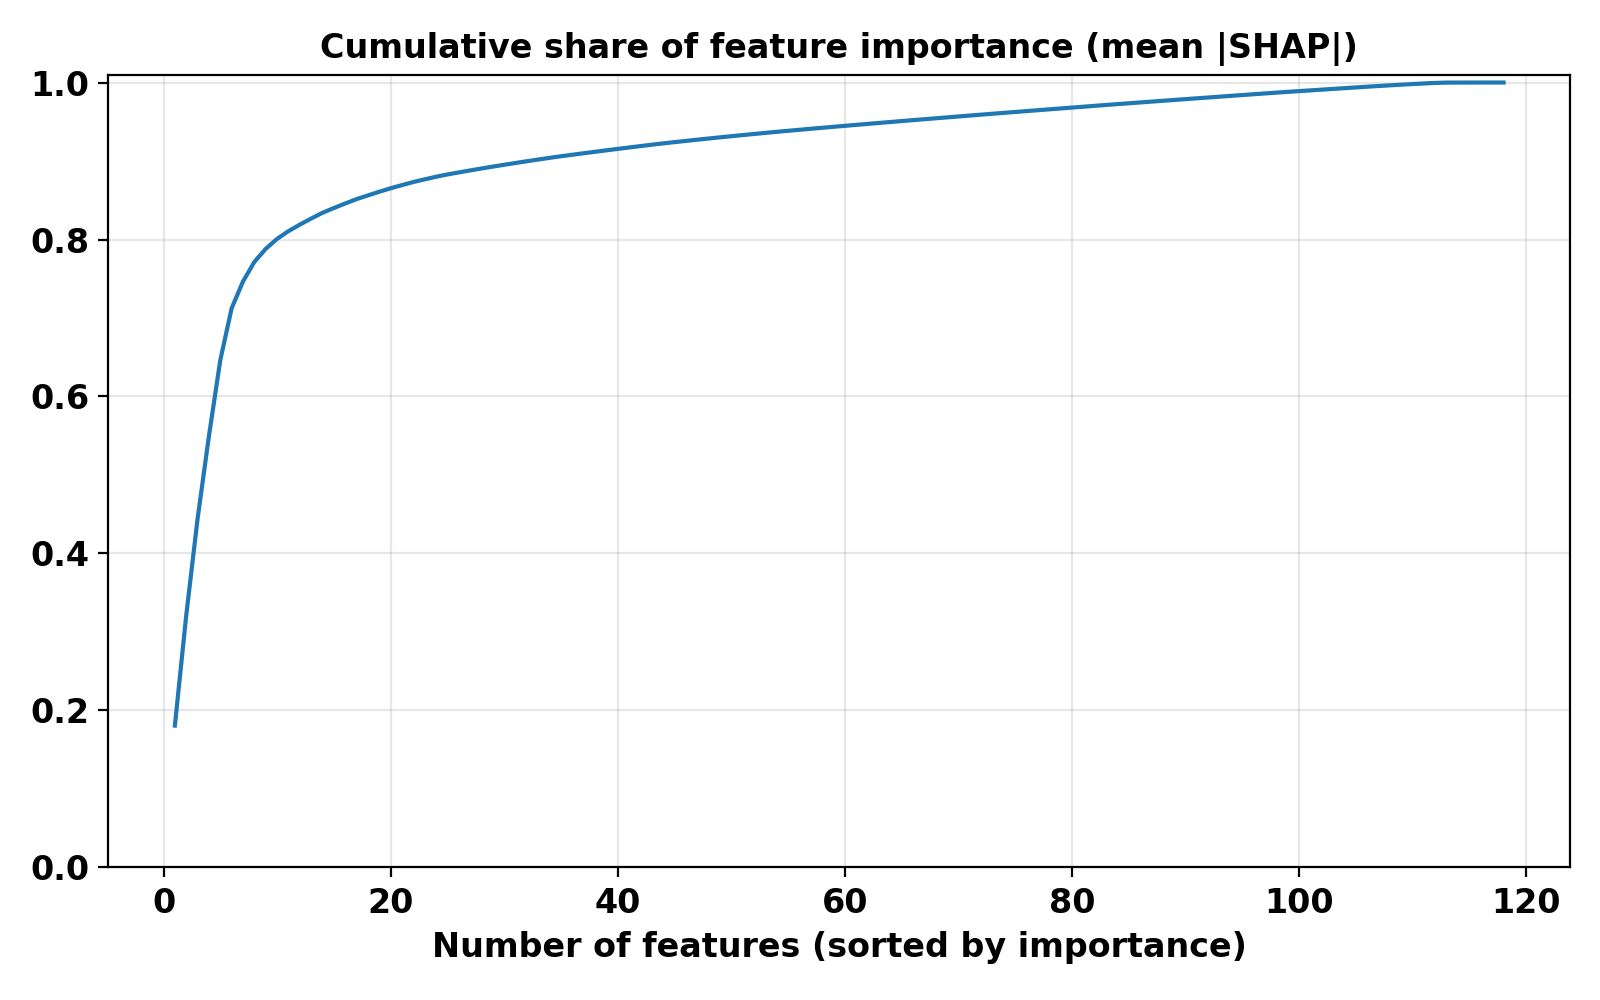
\includegraphics[width=\linewidth,height=6cm,keepaspectratio]{cumulative_importance_synth.png}
    \caption{All LIWC-2022 features (with synthetic data).}
    \label{fig:cum_synth_all}
  \end{subfigure}\hfill
  \begin{subfigure}[t]{0.49\textwidth}
    \centering
    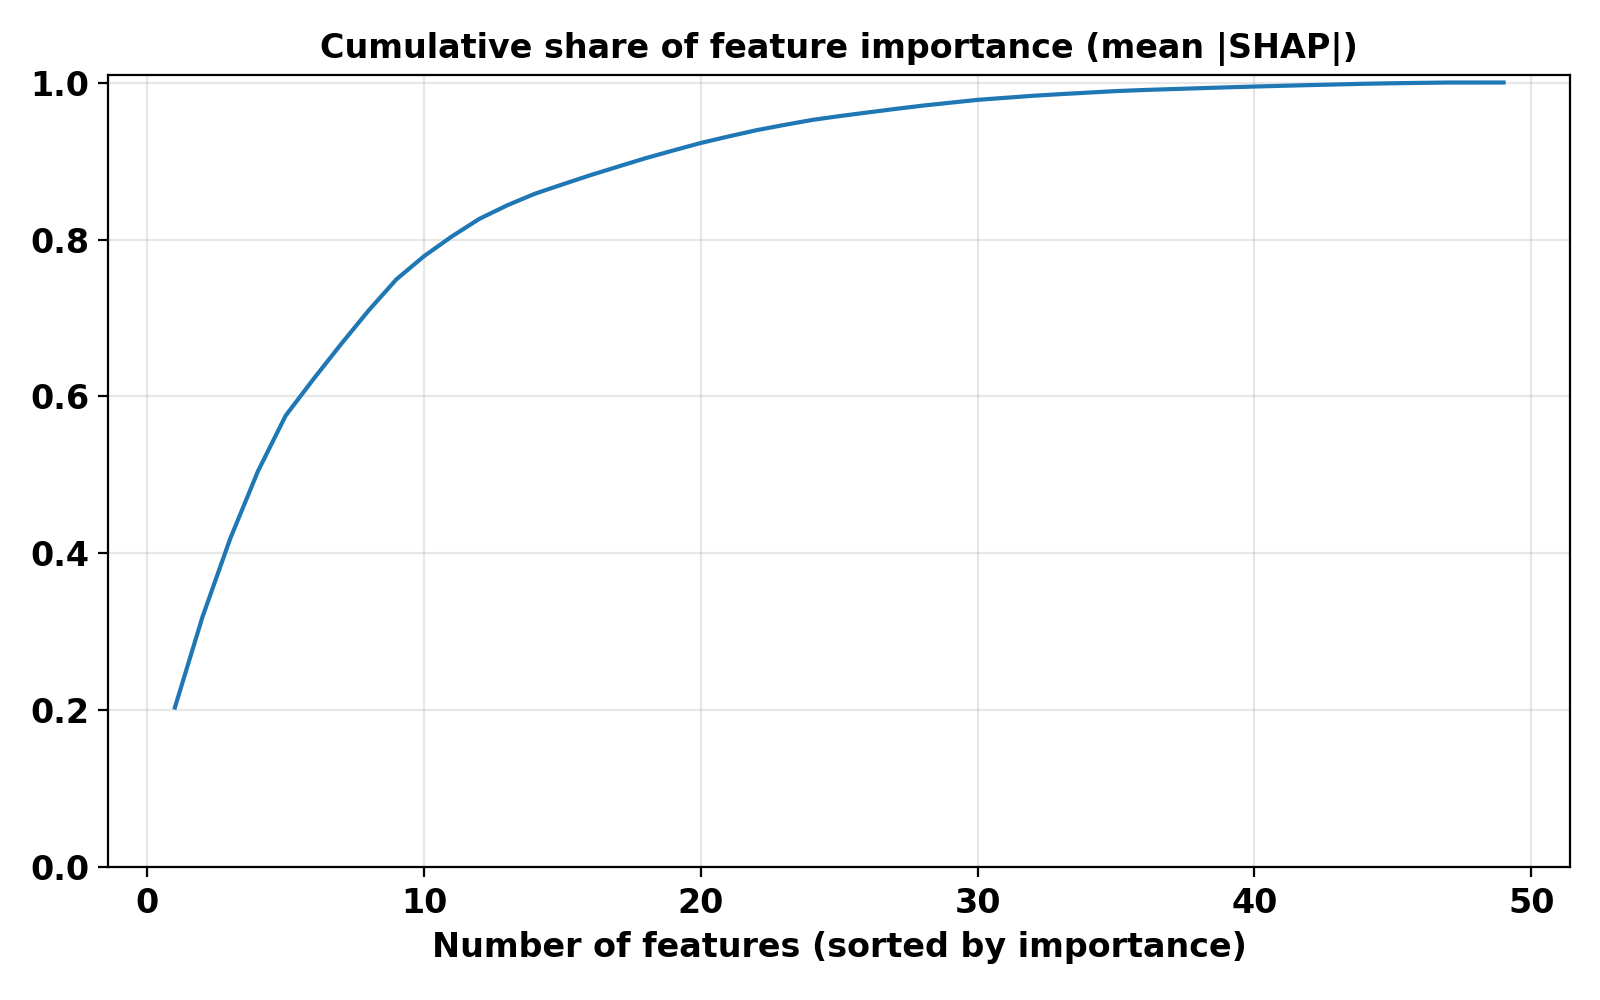
\includegraphics[width=\linewidth,height=6cm,keepaspectratio]{cumulative_importance_psycho_synth.png}
    \caption{Psychometric subset (with synthetic data).}
    \label{fig:cum_synth_psycho}
  \end{subfigure}
  
  \vspace{0.5cm}
  
  % Zweite Reihe: ohne synthetische Daten
  \begin{subfigure}[t]{0.49\textwidth}
    \centering
    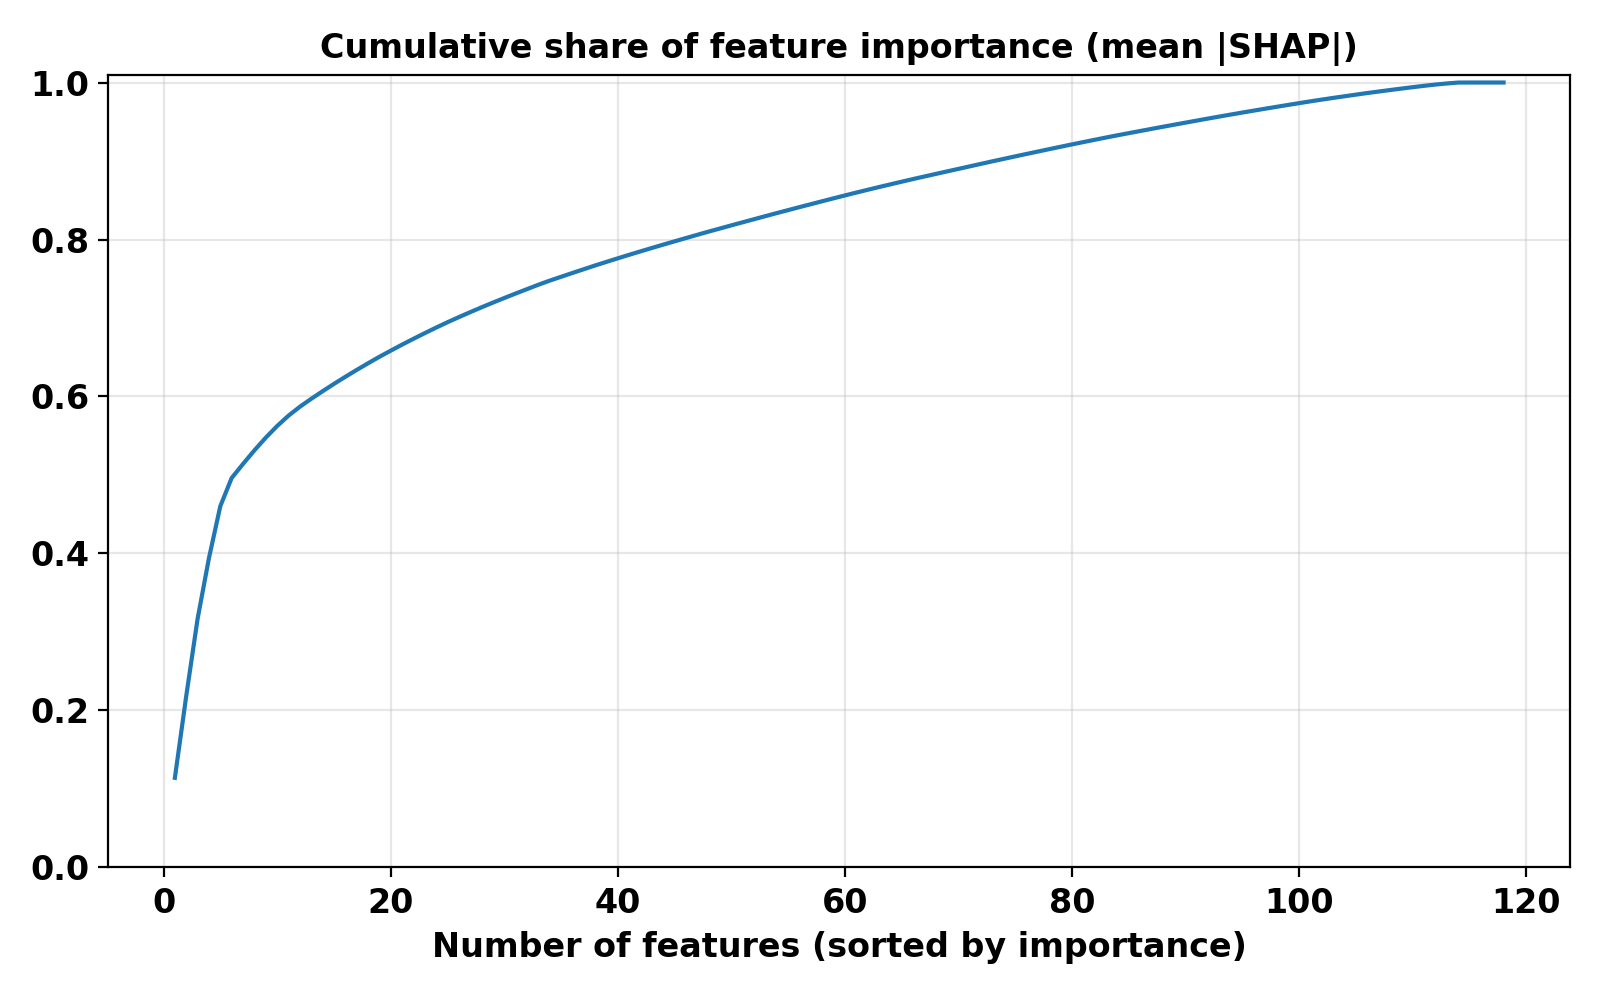
\includegraphics[width=\linewidth,height=6cm,keepaspectratio]{cumulative_importance_all_no_synth.png}
    \caption{All LIWC-2022 features (no synthetic data).}
    \label{fig:cum_no_synth_all}
  \end{subfigure}\hfill
  \begin{subfigure}[t]{0.49\textwidth}
    \centering
    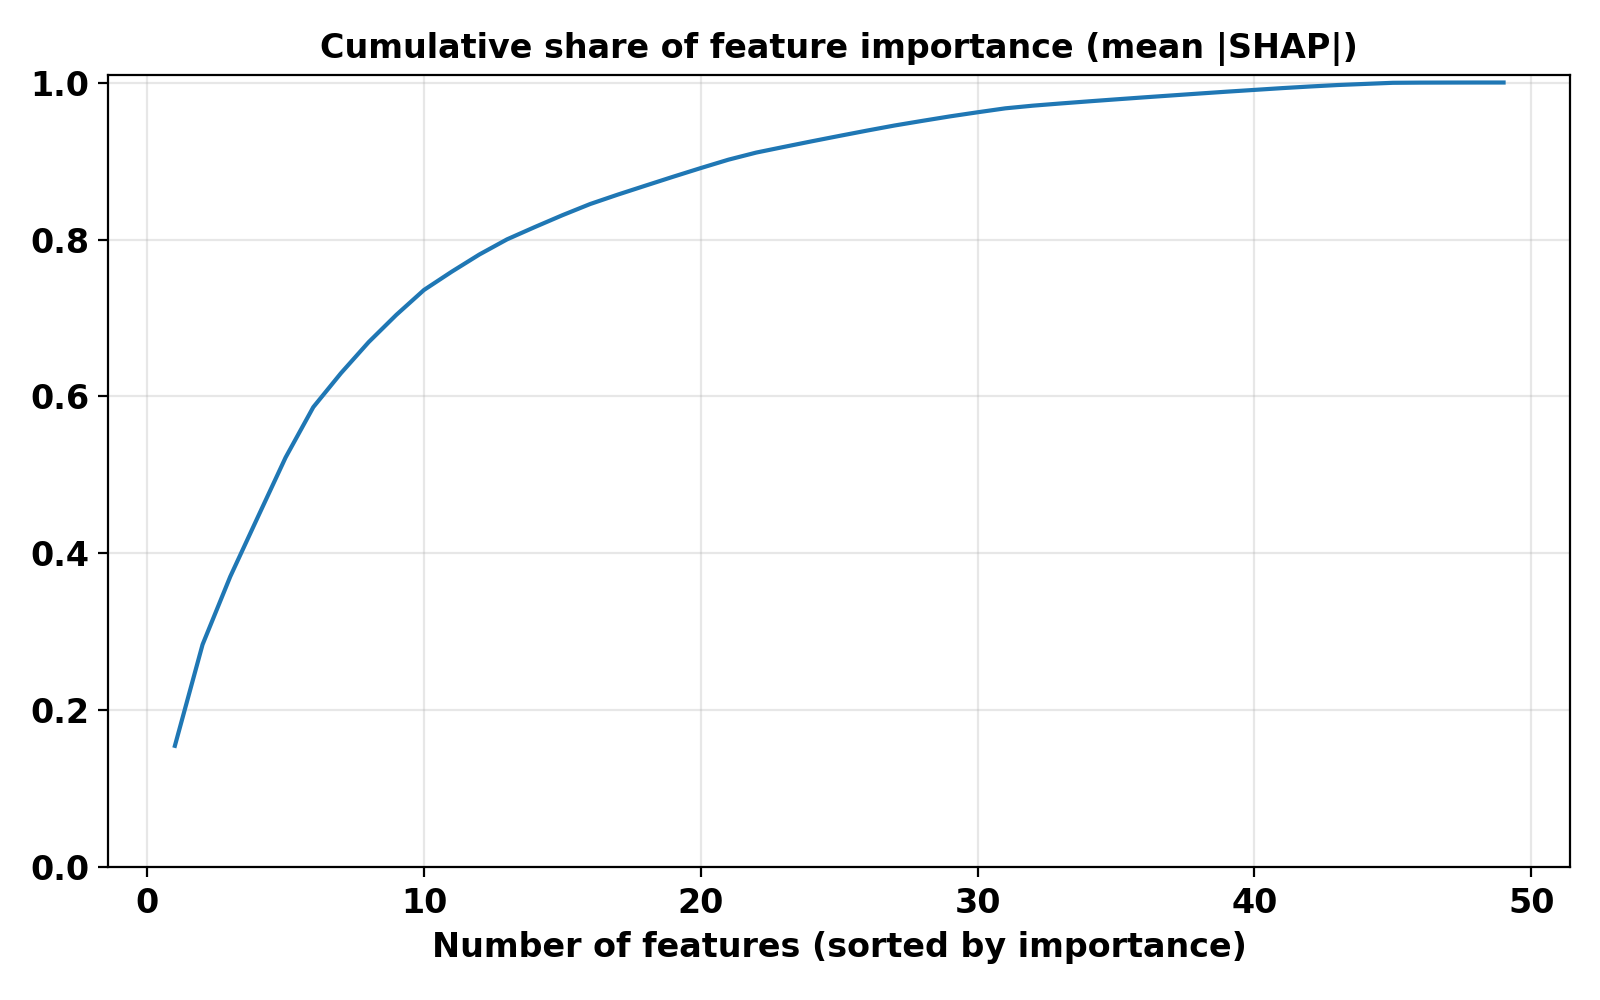
\includegraphics[width=\linewidth,height=6cm,keepaspectratio]{cumulative_importance_psycho_no_synth.png}
    \caption{Psychometric subset (no synthetic data).}
    \label{fig:cum_no_synth_psycho}
  \end{subfigure}

  \caption[Cumulative importance of LIWC-2022 features.]{\textbf{Cumulative importance of LIWC-2022 features.} 
  Top row: with synthetic data. Bottom row: no synthetic data.}
  \label{fig:cumulative_feature_importance_combined}
\end{figure}

When looking at the curves of the cumulative feature importance (Figure \ref{fig:cumulative_feature_importance_combined}), it is noticeable that the top 20 features already explain over 80\% of the model decision. This indicates, that the model relies strongly on a few key features to make its predictions. The two curves for the psychometric subset (with and without synthetic data) show an almost identical progression, suggesting that the inclusion of synthetic data does not alter the relative distribution of feature importance.\textbf{Note, that the smaller size of the psychometric subset feature size leads in an overall higher importance per feature compared to the full feature set, where the importance is distributed over a larger number of features.}


In comparison to the curves based on the psychometric subset, the curves based on all LIWC-2022 features show a more gradual increase, indicating that the model relies on a broader range of features to make its predictions. This is particularly evident when synthetic data is included, where the top 20 features explain only about 40\% of the model decision and the top 40 features explain about 60\%. In contrast, when no synthetic data is included, the top 20 features explain about 50\% of the model decision and the top 40 features explain about 70\% which is still a significant portion regarding the total amount of 118 features.This suggests, that the inclusion of synthetic data encourages the model to consider a wider array of features, potentially leading to improved generalization and robustness. Also, it is noticeable that the last 20 feature with the least importance in the full feature set explain only about 5\% of the model decision, indicating that these features contribute very little to the model's predictions and could potentially be excluded without significantly impacting the model performance.

To gain a deeper understanding of which specific LIWC features are the most influential in the model's decision-making process, a global ranking of the top 20 features was created based on their percentages of the total significance since the top 20 features hold the majority of the model's importance for both fusion configurations. The results are presented in the following Figure \ref{fig:global_feature_importance_combined}.


\begin{figure}[H]
  \centering
  
  % Erste Reihe: mit synthetischen Daten
  \begin{subfigure}[t]{0.49\textwidth}
    \centering
    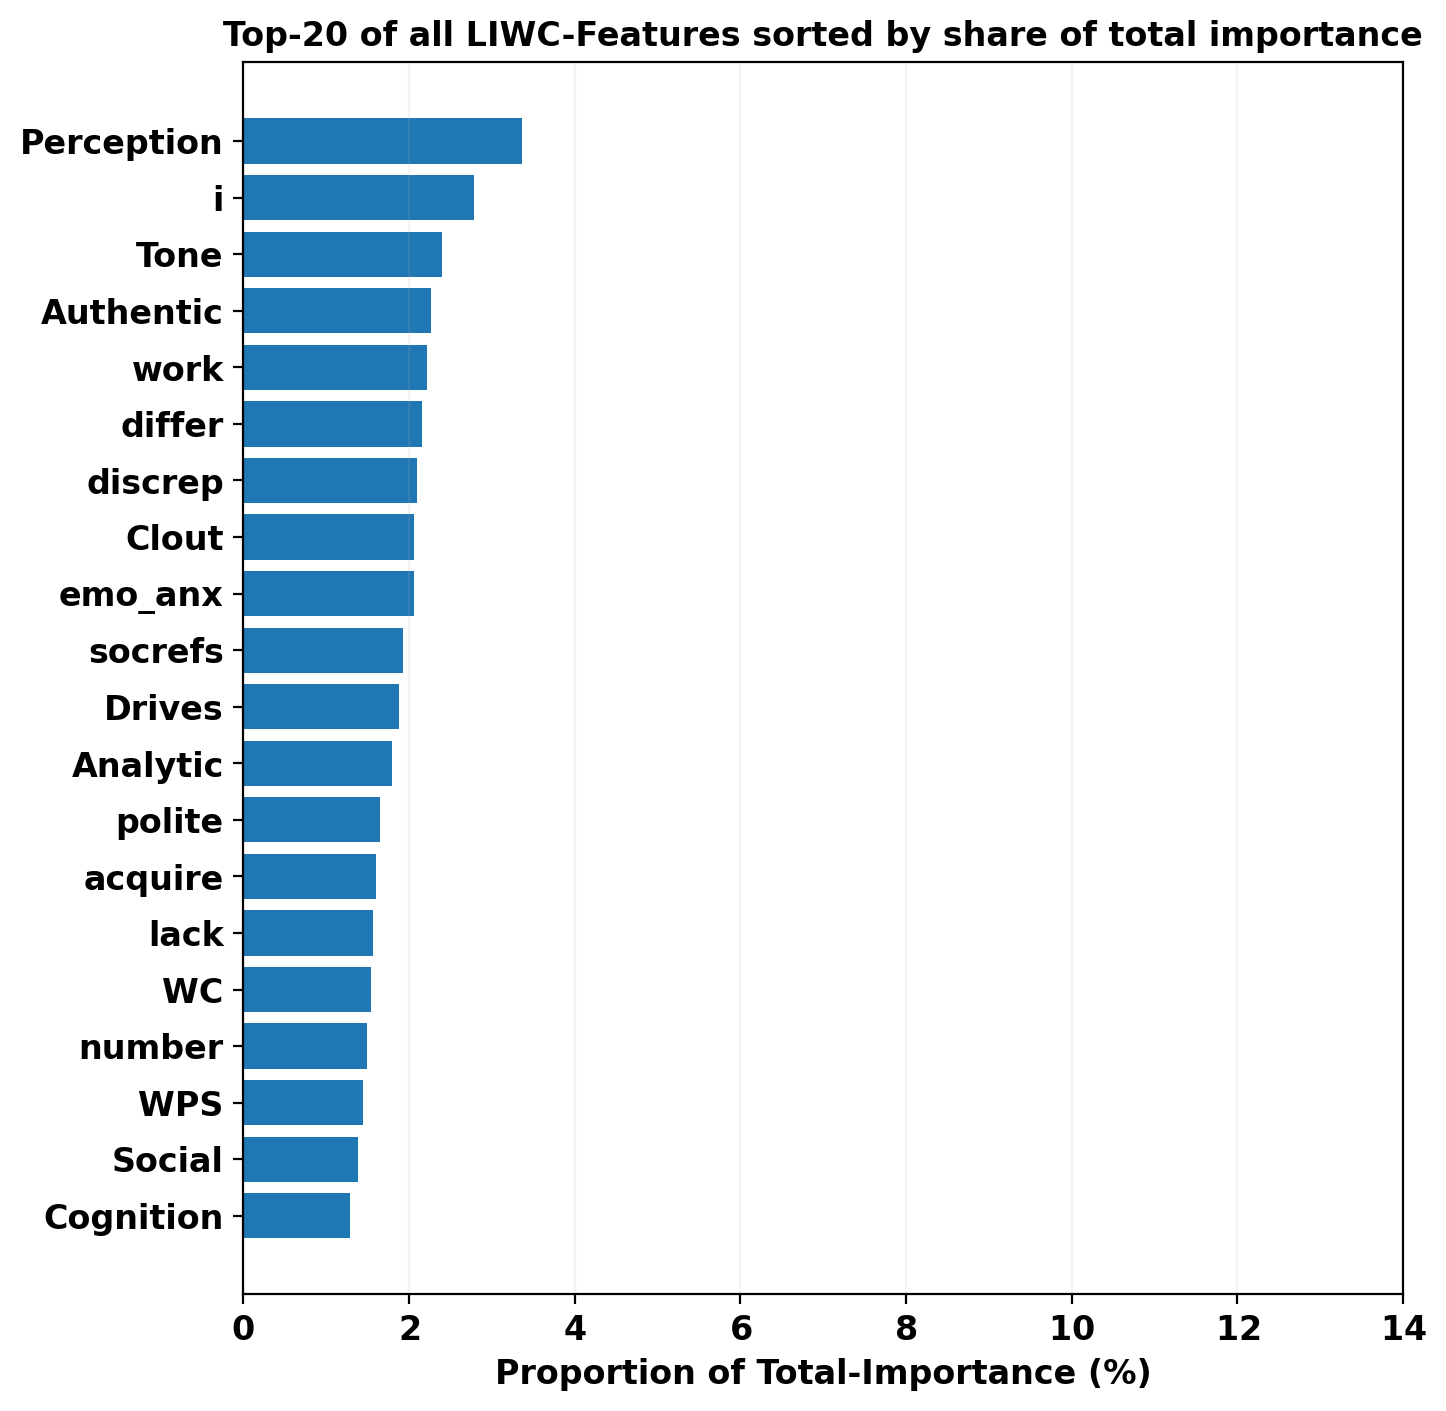
\includegraphics[width=\linewidth,height=6cm,keepaspectratio]{topN_share_importance_synth.png}
    \caption{All LIWC-2022 features (with synthetic data).}
    \label{fig:synth_all}
  \end{subfigure}\hfill
  \begin{subfigure}[t]{0.49\textwidth}
    \centering
    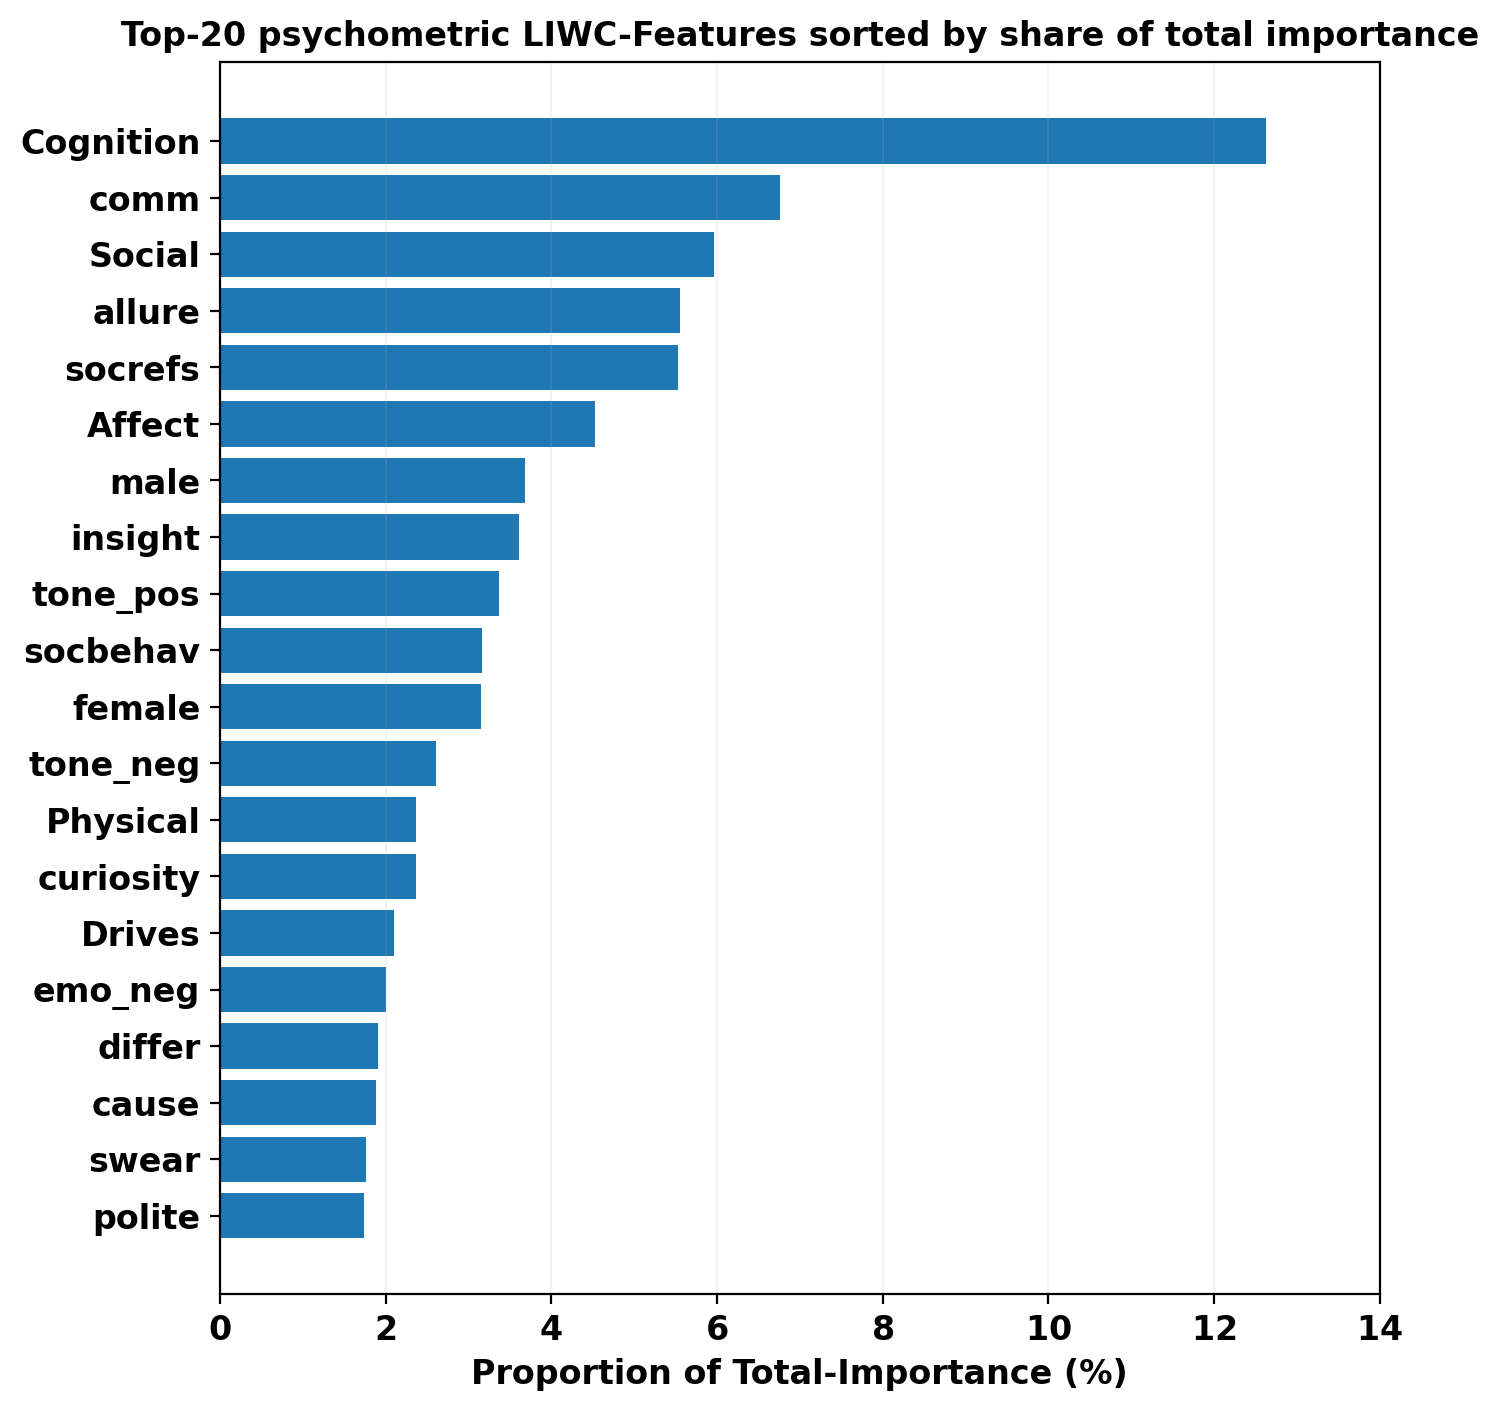
\includegraphics[width=\linewidth,height=6cm,keepaspectratio]{topN_share_importance_psycho_synth.png}
    \caption{Psychometric subset (with synthetic data).}
    \label{fig:synth_psycho}
  \end{subfigure}
  
  \vspace{0.5cm}
  

  \begin{subfigure}[t]{0.49\textwidth}
    \centering
    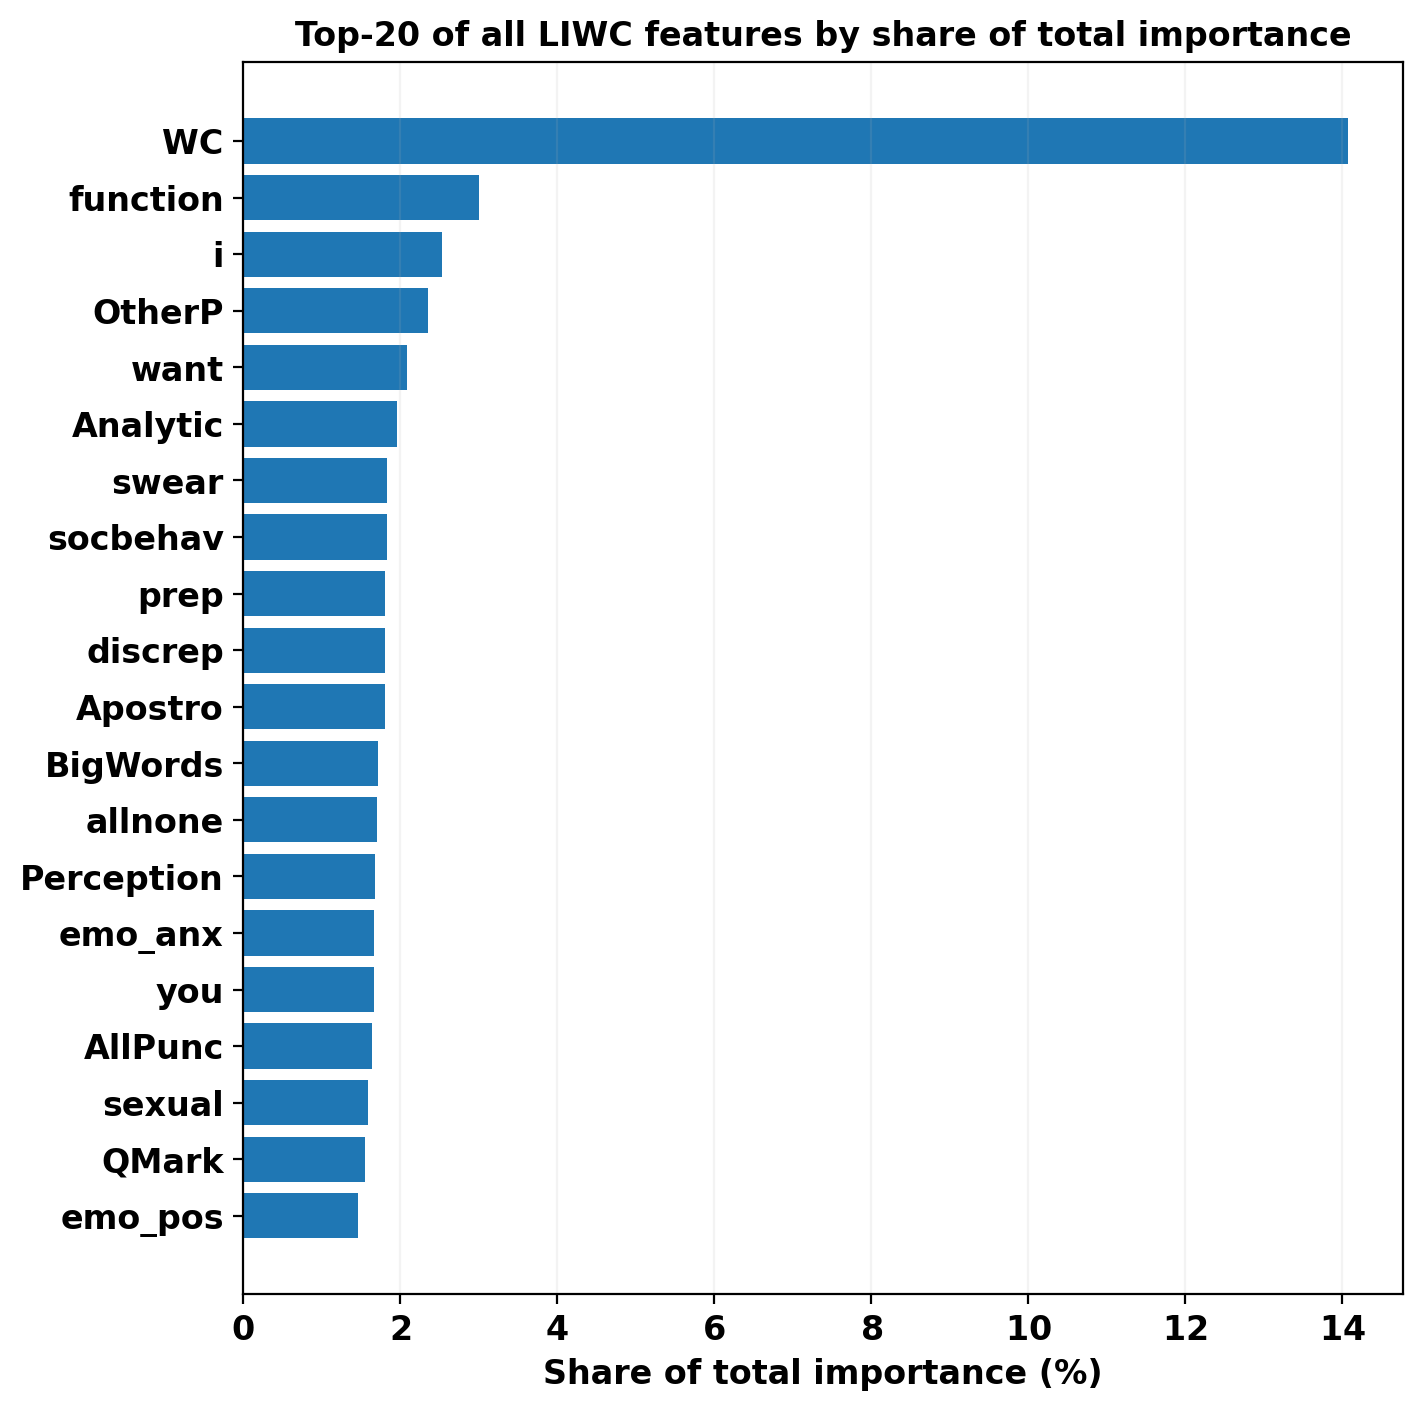
\includegraphics[width=\linewidth,height=6cm,keepaspectratio]{topN_share_importance_no_synth.png}
    \caption{All LIWC-2022 features (no synthetic data).}
    \label{fig:no_synth_all}
  \end{subfigure}\hfill
  \begin{subfigure}[t]{0.49\textwidth}
    \centering
    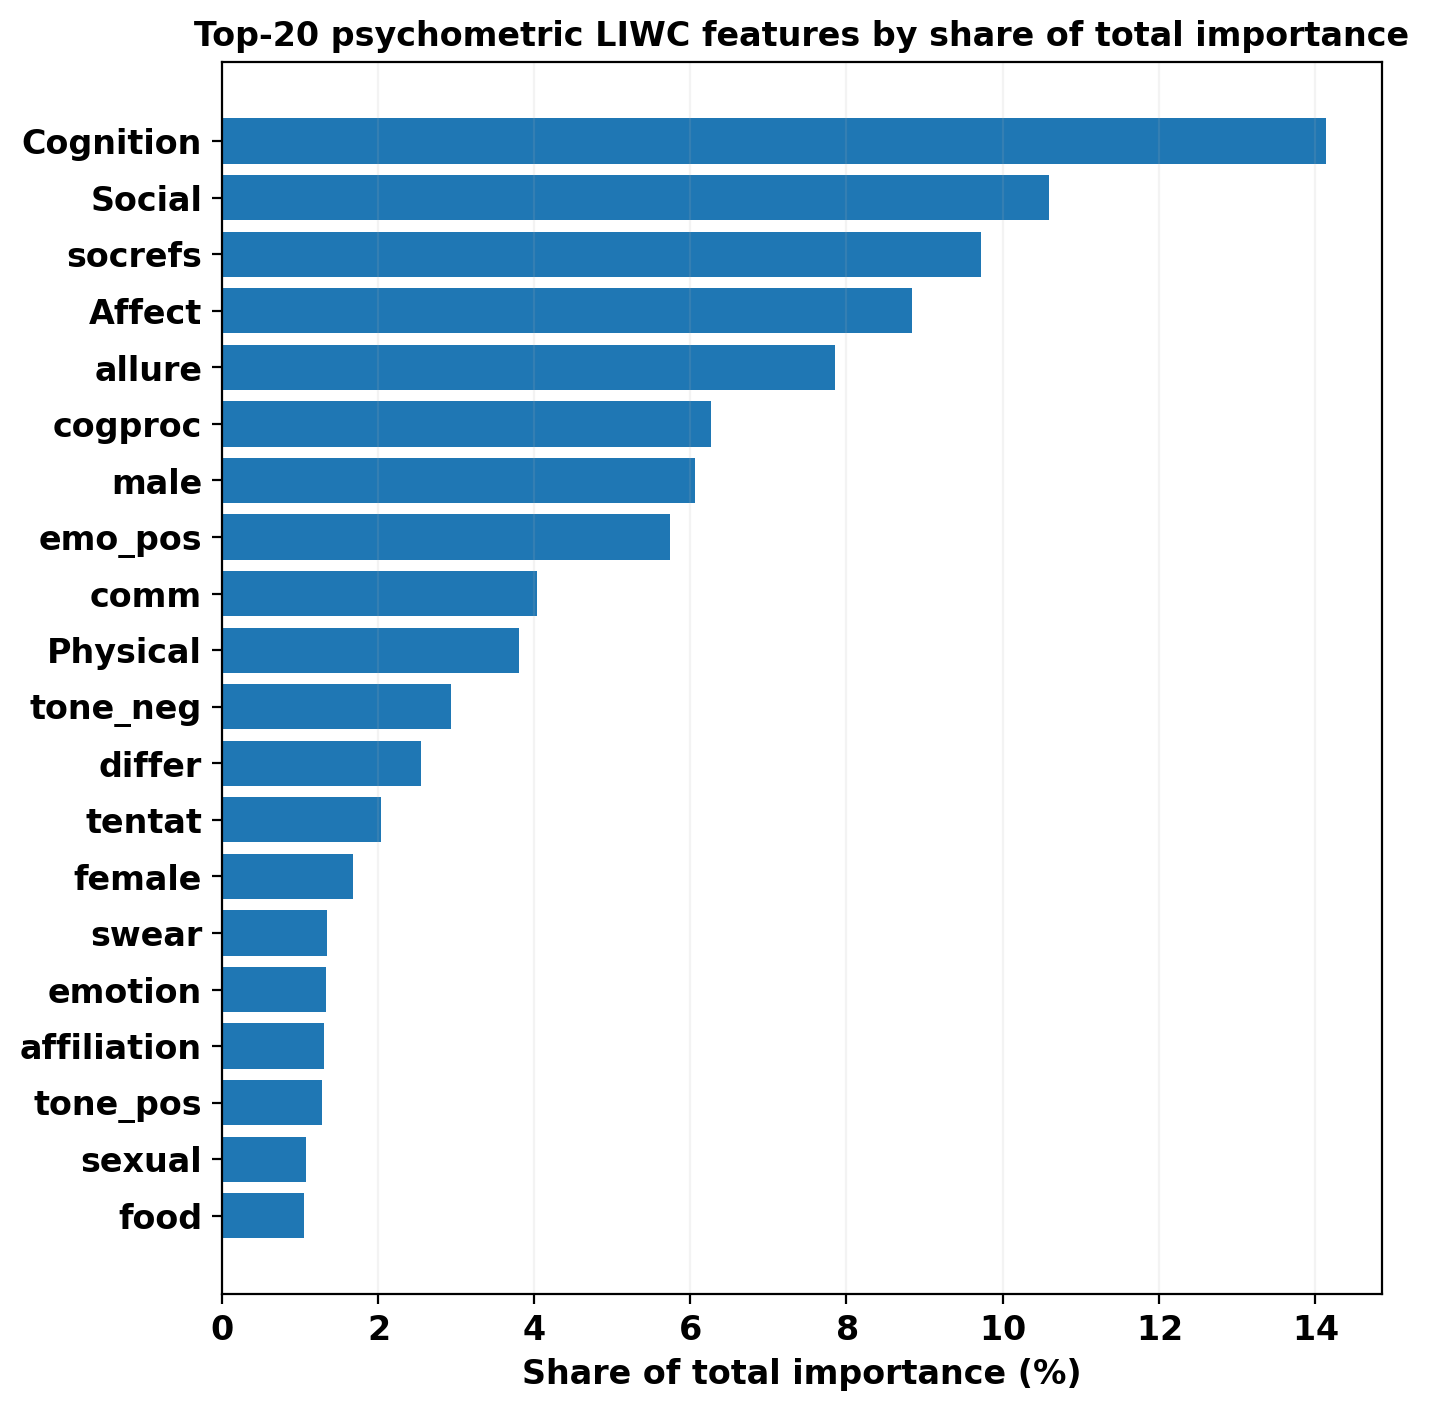
\includegraphics[width=\linewidth,height=6cm,keepaspectratio]{topN_share_importance_psycho_no_synth.png}
    \caption{Psychometric subset (no synthetic data).}
    \label{fig:no_synth_psycho}
  \end{subfigure}

  \caption[Top 20 LIWC features ranked by percentages of the total significance.]{\textbf{Top 20 LIWC features ranked by percentages of the total significance.} 
  Top row: with synthetic data. Bottom row: no synthetic data.}
  \label{fig:global_feature_importance_combined}
\end{figure}

The global rankings of the top 20 features (Figure~\ref{fig:global_feature_importance_combined}) confirm the observations from the cumulative curves. A comparatively small core of features contributes most to the model decision, with the type of features used differing between the full LIWC set and the psychometric subset, as well as between training with and without synthetic data.

\paragraph{All LIWC features (with synthetic data).}
\textbf{What is striking is a stronger weighting of \emph{content/psychological} categories like:} \textit{Perception}, \textit{i}, \textit{Tone}, \textit{Authentic}, \textit{Analytic}, \textit{Social}/\textit{Cognition} and relationship and status markers such as \textit{Clout} and \textit{polite}. Formal variables such as \textit{WC}, \textit{WPS} and \textit{number} also appear in the top 20, but are significantly less pronounced. \textbf{This suggests that synthetic data demonstrably reduces dependence on pure length signals and thus emphasizes semantic-psychological signals more}.

Note that, as already shown in the cumulative curves, the percentage feature importance per feature is generally lower for all LIWC features than in the psychometric subset. As already mentioned, this is probably explained by the generally larger feature set, which distributes the importance over a larger number of features that the model can rely on.

\paragraph{All LIWC features (without synthetic data).}
However, without synthetic data, \emph{formal} features dominate: \textit{WC} clearly ranks at the top, followed by \textit{function}, pronouns (\textit{i}, \textit{you}, \textit{OtherP}) and punctuation and word form features (\textit{AllPunc}, \textit{QMark}, \textit{Apostro}, \textit{BigWords}). Psychological categories (\textit{Analytic}, \textit{Perception}, \textit{emo\_anx}, \textit{sexual}) are present, but are clearly overshadowed by style and length indicators.
 

\paragraph{Psychometric subset (with synthetic data).}
Here, the focus is clearly on cognitive, social and affective processes such as \textit{Cognition} (dominant), \textit{tone_pos}, \textit{Social}, \textit{Physical}, \textit{cogproc}, \textit{Affect}, and \textit{insight}. In addition, features like \textit{comm}, \textit{socbehav}, \textit{tentat}, and \textit{cause} appear as secondary but consistent indicators. Compared to the configuration without synthetic data, the feature distribution is more top-heavy, with \textit{Cognition} showing a stronger dominance, suggesting that the model places greater emphasis on cognitive processes when synthetic samples are included.

\paragraph{Psychometric subset (without synthetic data).}
The ranking remains stable at its core (\textit{Cognition}, \textit{tone_pos}, \textit{Social}, \textit{cogproc}, \textit{Affect}), but the importance is more evenly distributed across the top features. This indicates that without synthetic data, the model relies on a broader but still consistent range of psychometric indicators. The stable dominance of cognitive and affective markers across both configurations suggests that reasoning, emotional tone, and social orientation are key discriminators between grooming and non-grooming dialogues.

To further gain insights into the direction of the effects of the individual features, the mean signed SHAP values were visualized in the following section.


\subsubsection{Singed Feature Importance by Class}

\begin{figure}[H]
  \centering
  
  % Erste Reihe: mit synthetischen Daten
  \begin{subfigure}[t]{0.49\textwidth}
    \centering
    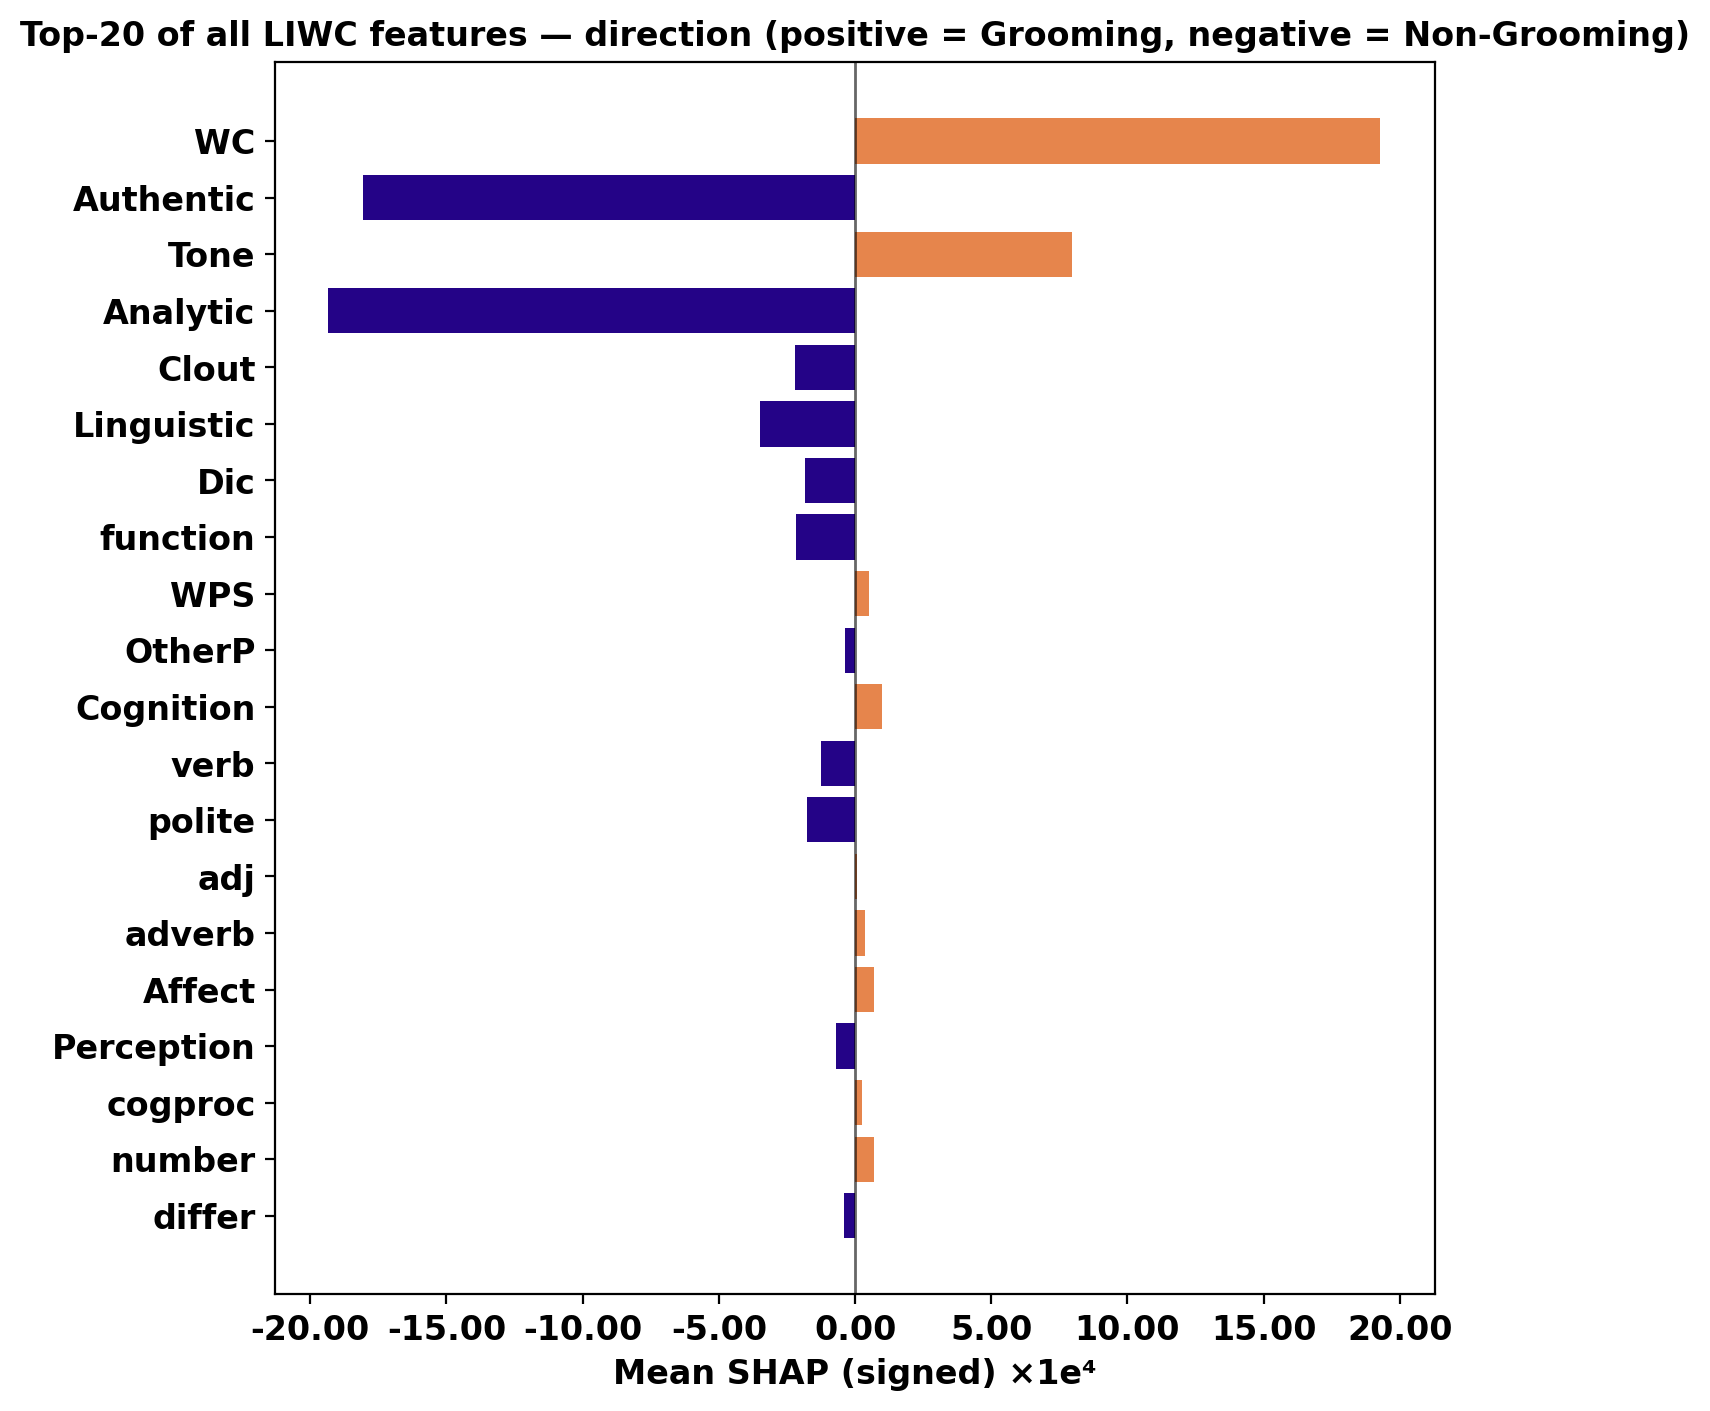
\includegraphics[width=\linewidth,height=6cm,keepaspectratio]{topN_mean_signed_importance_synth.png}
    \caption{All LIWC-2022 features (with synthetic data).}
    \label{fig:synth_all_shap}
  \end{subfigure}\hfill
  \begin{subfigure}[t]{0.49\textwidth}
    \centering
    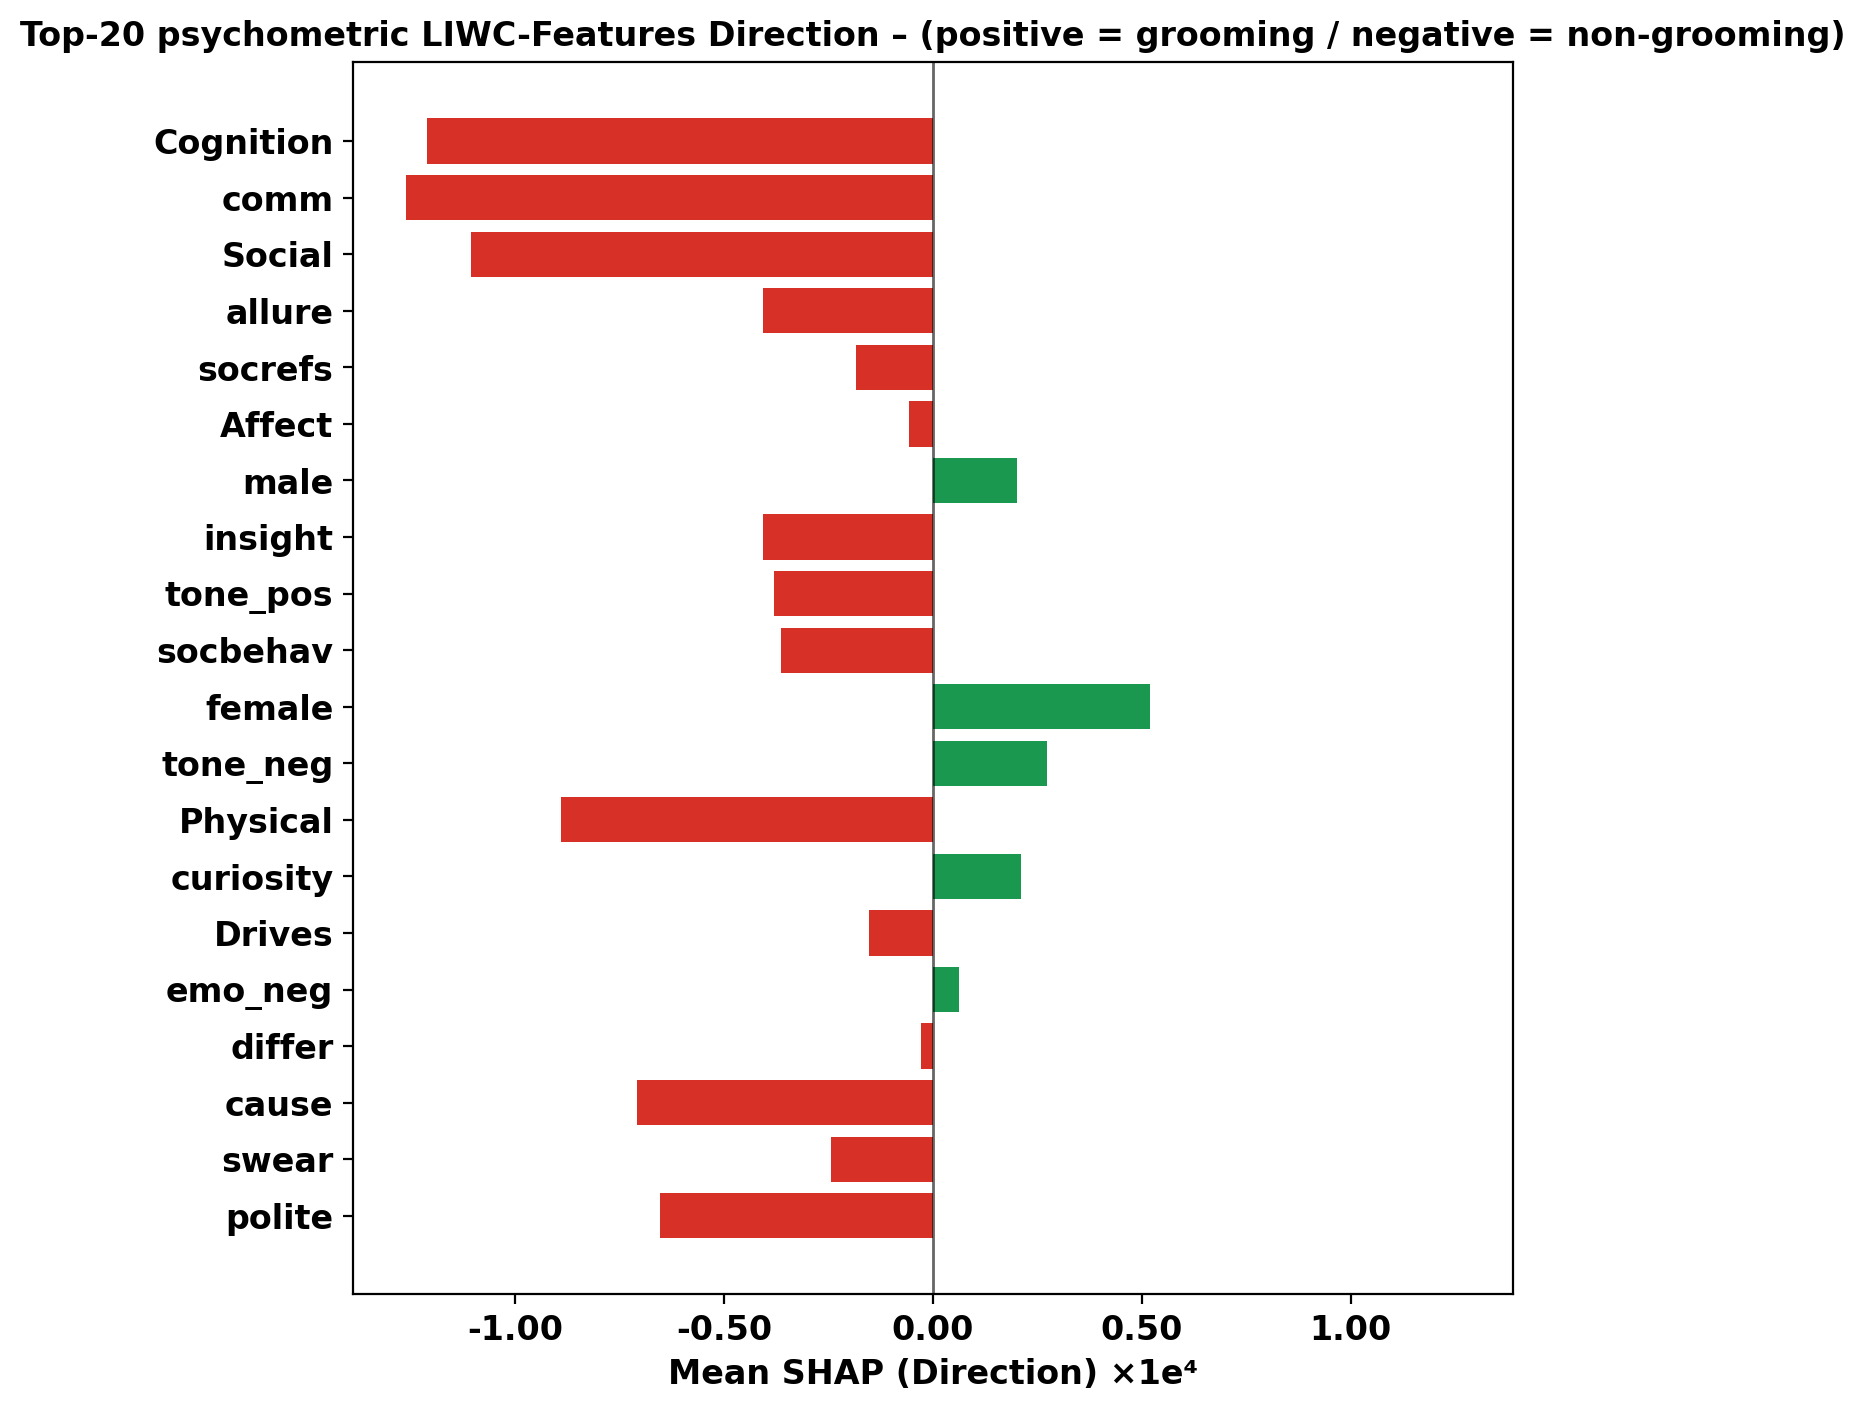
\includegraphics[width=\linewidth,height=6cm,keepaspectratio]{topN_mean_signed_importance_psycho_synth.png}
    \caption{Psychometric subset (with synthetic data).}
    \label{fig:synth_psycho_shap}
  \end{subfigure}
  
  \vspace{0.5cm}
  
  % Zweite Reihe: ohne synthetische Daten
  \begin{subfigure}[t]{0.49\textwidth}
    \centering
    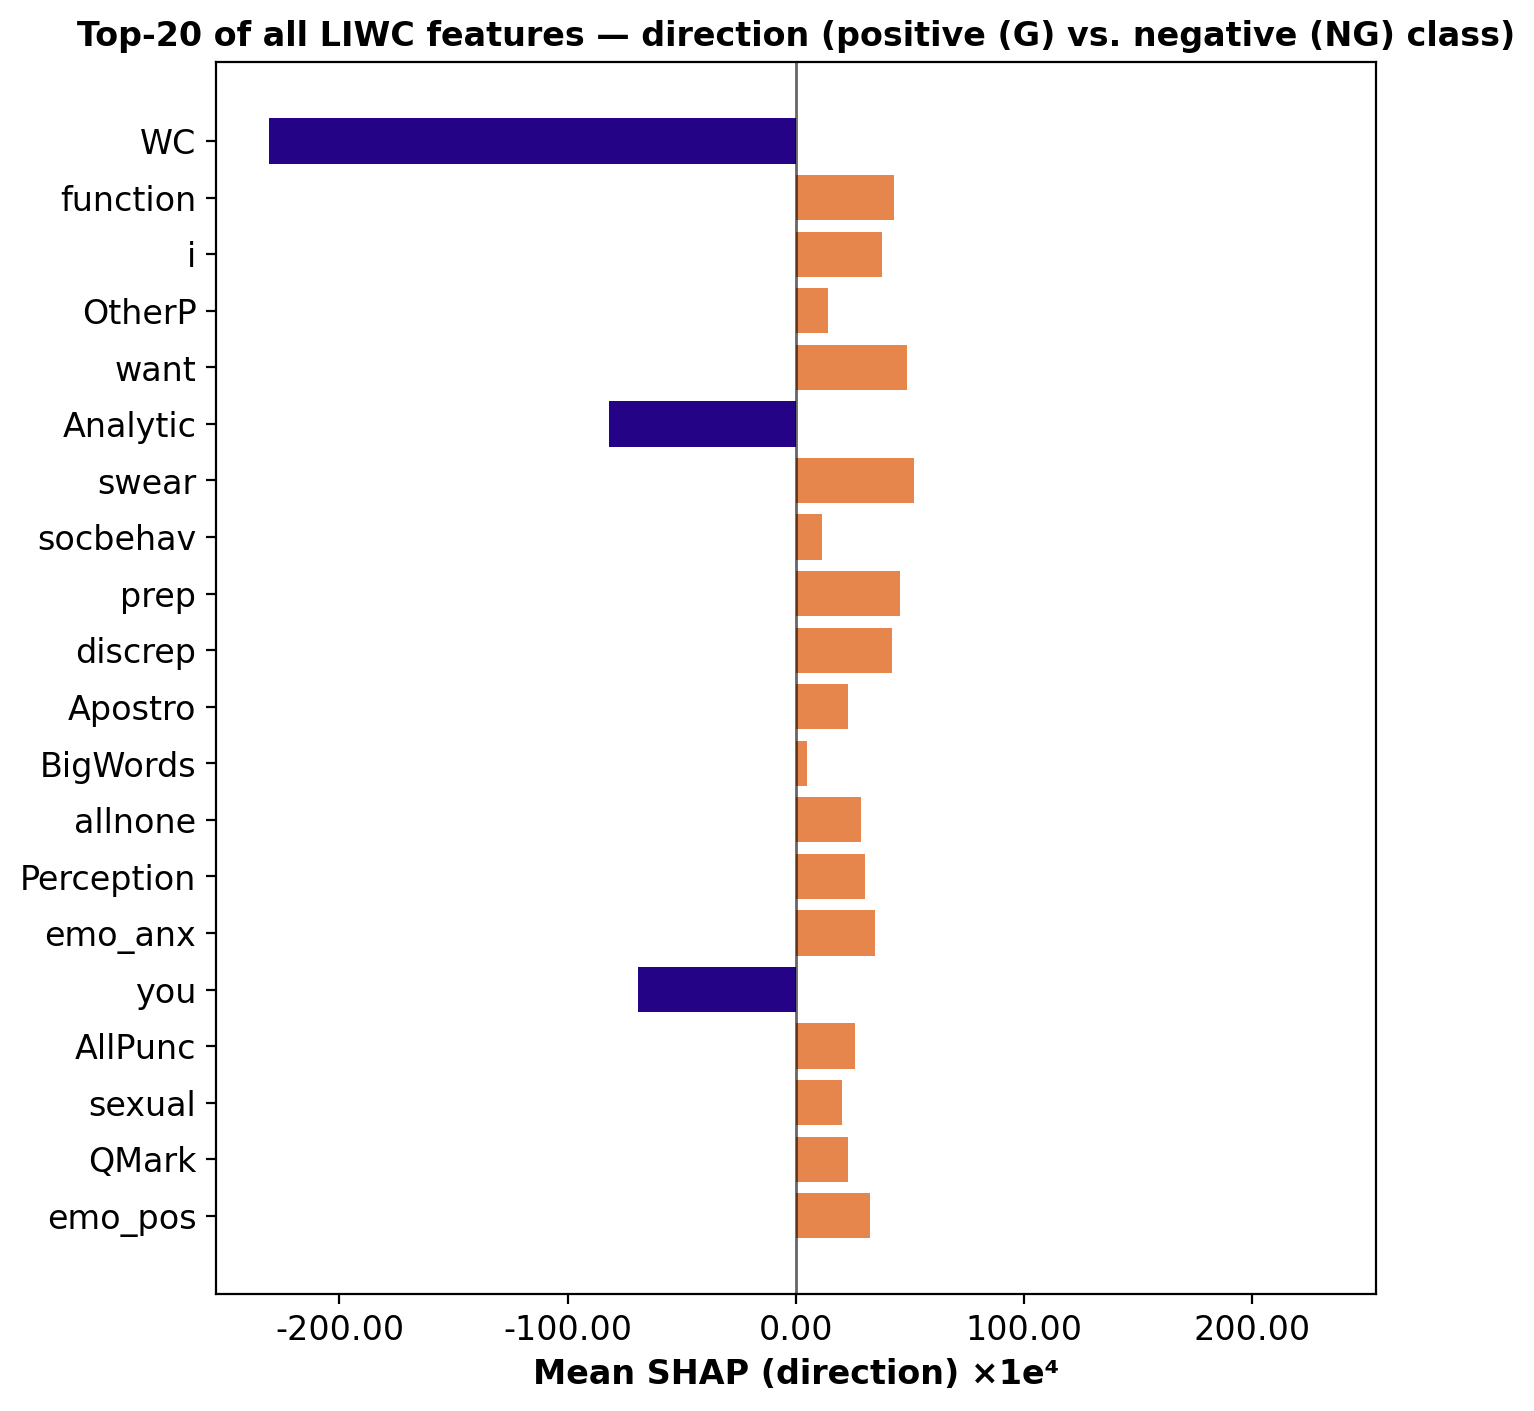
\includegraphics[width=\linewidth,height=6cm,keepaspectratio]{topN_mean_signed_importance_all_no_synth.png}
    \caption{All LIWC-2022 features (no synthetic data).}
    \label{fig:no_synth_all_shap}
  \end{subfigure}\hfill
  \begin{subfigure}[t]{0.49\textwidth}
    \centering
    \includegraphics[width=\linewidth,height=6cm,keepaspectratio]{topN_mean_signed_importance_psycho_no_synth.png}
    \caption{Psychometric subset (no synthetic data).}
    \label{fig:no_synth_psycho_shap}
  \end{subfigure}

  \caption[Top 20 LIWC features ranked by mean signed SHAP value.]{\textbf{Top 20 LIWC features ranked by mean signed SHAP value.} 
  Top row: with synthetic data. Bottom row: no synthetic data. 
  Positive values indicate a shift toward the grooming class, negative values toward the non-grooming class. 
  \textit{Note: the scales differ between the plots. The left-hand plots (all features) have a larger range than the right-hand plots (psychometric subset).}}
  \label{fig:feature_importance_by_class_combined}
\end{figure}

Figure \ref{fig:feature_importance_by_class_combined} shows the top 20 LIWC features ranked by their mean signed SHAP values for both configurations (all LIWC-2022 features and psychometric subset) with and without synthetic data. Note, that the mean signed Feature plots show the same features as the global importance plots, but now colored by their direction of effect. Positive values indicate a shift toward the grooming class, negative values toward the non-grooming class. \textbf{However, the direction (positive = grooming, negative = non-grooming in the plots) does not mean that “high” values of a feature always have this effect. Rather, it shows that deviations of the feature from the average contribute to the prediction in this direction.}
Using the example of \textbf{Word Count}: If the feature indicates non-grooming, this does not automatically mean “high word count = non-grooming.” It can just as easily mean that both high and low values, depending on the context, indicate non-grooming. The plot simply summarizes these effects as an average contribution across all data points considered.

\textbf{ It is also striking, that the SHAP results indicate that several features change their direction when synthetic data are included, suggesting that the feature attribution is sensitive to the underlying data composition.} This is particularly evident in the psychometric subset, where top features like \textit{Cognition} and \textit{tone_pos} shift the direction of their effect when synthetic data is included. It is important to mention, that the underlying training data remain identical across both analyses. These changes in SHAP directionality are caused by differences in the explained sample set and background distribution, for example, whether synthetic data were included in the explanation phase or filtered out. \textbf{Since SHAP values are computed relative to a background distribution, even small changes in data composition can shift the baseline and therefore the average feature contributions.} 

\paragraph{Note on axis scaling (effect magnitudes).}
The x-axis (mean \emph{signed} SHAP value) is scaled very differently across panels. In particular, \emph{All LIWC-2022 features (with synthetic data)} spans roughly $[-200,+200]\times 10^{4}$, whereas \emph{Psychometric subset (no synthetic data)} spans about $[-10,+10]\times 10^{4}$ and \emph{Psychometric subset (with synthetic data)} about $[-1,+1]\times 10^{4}$. 
Thus, absolute effects are \emph{much larger} in the "All LIWC + synthetic" panel, even when bars look visually similar, followed by the psychometric/no-synthetic panel and, lastly, the psychometric/with-synthetic panel. 
Consequently, bar lengths should be compared primarily \emph{within} a panel and not in between. For cross-panel comparisons, only focus on \emph{direction} (sign) and \emph{ranking}.

\paragraph{Interpretation of directional effects.}
Instead of listing individual features, Figure~\ref{fig:feature_importance_by_class_combined} reveals a pattern according to which dialogues are classified as grooming or non-grooming:

Language characterized by \emph{cognitive-reflexive and cooperative} patterns (planning, explaining, referencing conversation partners, polite and positive tone) tends to deviate in ways that shift the decision toward \textbf{non-grooming}. In contrast, \emph{emotionally charged, boundary-testing and closeness creating} patterns (tense tone, heightened affect, uncertainty/consideration, targeted information gathering or “luring” and explicit sexual references) show deviations that shift the decision toward \textbf{grooming}. This picture complements the global and cumulative analyses of the previous sections. The separation is here mainly driven by content related psychological processes, while formal textual deviations (length, punctuation) act as stronger indicators especially in the absence of synthetic data.

\paragraph{All features with vs. without synthetic data.}
With synthetic data, the \emph{semantic-psychological} contrast becomes more apparent. Here, deviations reflecting cognitively and socially ordered and positive conversation tend to shift predictions toward non-grooming, while deviations in tonal/affective tension, authenticity/status cues and questioning patterns (e.g., about age/contact) shift predictions toward grooming. Without synthetic data, however, the model more often relies on \emph{formal proxies} such as text length or punctuation deviations for non-grooming, while grooming predictions are composed of many smaller stylistic-affective deviations. This shift toward formal characteristics explains the steeper cumulative importance without synthetic data and underscores the risk of spurious correlations.

\paragraph{Psychometric subset with vs. without synthetic data.}
In the psychometric space, the directional effects are particularly plausible. Deviations linked to \emph{cognition, cooperation, and positive tone} tend to support non-grooming, while deviations related to \emph{negative affect, intensified tone, boundary testing/uncertainty, and intimate context markers} tend to support grooming. With synthetic data, ambivalent categories (such as “compliments/allure” or vulgar language markers) are smoothed and lose their strong one-sided association with grooming. Without synthetic data, sharper contrasts emerge, and grooming- and boundary-testing deviations come more clearly to the fore. The cumulative curves in Figure~\ref{fig:cumulative_feature_importance_combined} illustrate this: synthetic data distribute importance more evenly, while real-only data concentrate importance on a few pronounced deviations.




\section{Confidence Analysis and Label Flip Analysis} \label{sec:confidence_and_label_flip_analysis}

In addition to the performance metrics and feature importance analysis, further evaluations were conducted to analyze the model's confidence in its predictions and to analyze instances where the model's predictions changed between evaluations after using LIWC features als additional model Inputs. This analysis was conducted on the dataset including synthetic data to assess the overall behavior of the model with and without LIWC features. \textbf{For the analysis, a total of 6849 samples were evaluated to reduce computational effort.}

\begin{figure}[H]
  \centering
  
  % All features
  \begin{subfigure}[t]{0.49\textwidth}
    \centering
    \includegraphics[width=\linewidth,height=6cm,keepaspectratio]{confidence_analysis_plots/maxprob_scatter.png}
    \caption{Confidence shift analysis for all LIWC-2022 features.}
    \label{fig:confshift_all}
  \end{subfigure}\hfill
  % Psychometric subset
  \begin{subfigure}[t]{0.49\textwidth}
    \centering
    \includegraphics[width=\linewidth,height=6cm,keepaspectratio]{confidence_analysis_psycho_plots/maxprob_scatter.png}
    \caption{Confidence shift analysis for psychometric LIWC-2022 subset.}
    \label{fig:confshift_psycho}
  \end{subfigure}

  \caption[Confidence shift analysis with LIWC features.]{\textbf{Confidence shift analysis with LIWC features.} 
  Left: all LIWC-2022 features. Right: psychometric subset of LIWC-2022 features. 
  Both plots show model confidence with LIWC set to zero (x-axis) versus LIWC as-is (y-axis). 
  The diagonal indicates no effect. 
  Points above the diagonal correspond to increased confidence due to LIWC features, while points below indicate reduced confidence. 
  The farther a point lies from the diagonal, the stronger the influence of LIWC features on model confidence. }
  \label{fig:confidence_shift}

\end{figure}


When looking on figure \ref{fig:confidence_shift} it can been seen that for all LIWC-2022 features (left), a lot of samples lie above the diagonal, indicating that the model's confidence in its predictions increased when LIWC features were included. Also, most of the samples lie close to the upper border (0.9 - 1.0) indicating an overall really high confidence of the model in its predictions using all LIWC-2022 features.
This suggests that the additional information provided by the full LIWC feature set helps the model make more confident predictions in most of the cases. Note that there are also some points underneath the diagonal showing that in some cases the model confidence decreased when LIWC features were included. 

When looking on the psychometric subset of LIWC-2022 features (right), a similar pattern can be observed, but the effect is less pronounced. While there are still many points above the diagonal indicating increased confidence, the points are more widely spread and lie closer to the diagonal, suggesting that the impact of the psychometric subset on model confidence is more moderate compared to using all LIWC features. This indicates that while the psychometric features are still valuable, they may not provide as much additional information as the full feature set.

The following table \ref{tab:confidence_label_flip} additionally shows the results of the confidence and label flip analysis for both the complete LIWC-2022 feature set and the psychometric subset after analyzing 6849 samples.

\begin{table}[H]
\centering
\caption{Confidence and label flip analysis for all LIWC-2022 features vs. psychometric subset.}
\begin{tabular}{lcc}
\toprule
\textbf{Metric} & \textbf{All Features} & \textbf{Psychometric Subset} \\
\midrule
Number of samples ($n$)            & 6849    & 6849 \\
$\Delta \mu$ (mean)                & 0.1543  & 0.0219 \\
$\Delta \tilde{x}$ (median)        & 0.2363  & 0.0313 \\
$\Delta \sigma$ (std)              & 0.1481  & 0.0256 \\
$\Delta p_{10}$                    & -0.0166 & -0.0020 \\
$\Delta p_{90}$                    & 0.3081  & 0.0454 \\
Class 0 count                      & 4055    & 3942 \\
Class 1 count                      & 2794    & 2907 \\
Flipped predictions                & 156     & 9 \\
Flip rate                          & 0.0228  & 0.0013 \\
\bottomrule
\end{tabular}
\label{tab:confidence_label_flip}
\end{table}

Additionally the Agreeement matrices for the model with all LIWC-2022 features and the psychometric subset are shown in the following figure: 
\begin{figure}[H]
  \centering

  % All features
  \begin{subfigure}[t]{0.49\textwidth}
    \centering
    \includegraphics[width=\linewidth,height=6cm]{confidence_analysis_plots/confusion_predtrue_vs_predzero.png}
    \caption{Agreement matrix for all LIWC-2022 features.}
    \label{fig:agreement_all}
  \end{subfigure}\hfill
  % Psychometric subset
  \begin{subfigure}[t]{0.49\textwidth}
    \centering
    \includegraphics[width=\linewidth,height=6cm]{confidence_analysis_psycho_plots/confusion_predtrue_vs_predzero.png}
    \caption{Agreement matrix for psychometric LIWC-2022 subset.}
    \label{fig:agreement_psycho}
  \end{subfigure}

  \caption[Agreement matrices for predictions with vs. without LIWC features.]{\textbf{Agreement matrices for predictions with vs. without LIWC features.} 
  Left: all LIWC-2022 features. Right: psychometric subset of LIWC-2022 features. 
  Each matrix compares the predicted class with LIWC features (y-axis) against the prediction without LIWC features (x-axis). 
  Values on the diagonal indicate stable predictions, while off-diagonal values represent \emph{label flips}.}
  \label{fig:agreement_combined}
\end{figure}

When looking at table \ref{tab:confidence_label_flip}, it can be seen that the model with all LIWC-2022 features shows a much stronger confidence shift (mean increase of 0.1543) compared to the psychometric subset (mean increase of 0.0219). This indicates again, that adding the full LIWC feature set has a more pronounced effect on the models confidence in its predictions. The median values also reflect this trend, with a larger increase for the full feature set (0.2363) compared to the subset (0.0313). The standard deviation is higher for the full feature set (0.1481) than for the subset (0.0256), suggesting greater variability in confidence shifts when using all features which is also reflected when looking at the samples in figure \ref{fig:confidence_shift}. 

Also, the model with the complete LIWC-2022 Feature set seems to have a higher amount of label flip, flipping 156 prediction labels in total from Label Grooming to label Non-Grooming. In comparison, the model using only the psychometric subset of LIWC features has this kind of label flip. This indicates that the inclusion of all LIWC-2022 features leads to more changes in the model's predictions, which could be due to the additional information provided by a higher amount of LWIC-Features.

\textbf{Note, that there is only a label flip direction of Grooming to Non-Grooming, but not the other way around.} This suggests that the LIWC features help the model to be more conservative in its predictions, reducing false positives by reclassifying some grooming predictions as non-grooming. Also, when looking at the total amount of samples which were analyzed (6849 in total), the number of label flips is relatively small (2.28\% for all features and 0.13\% for the psychometric subset), indicating that the model's predictions are generally stable even when LIWC features are not included.

Overall, these results suggest that while both configurations enhance model confidence, the full LIWC-2022 feature set has a more substantial impact on both confidence shifts and prediction stability.


\section{Missclassification Analysis based on LIWC-Scores} \label{sec:misclassification_analysis}


\subsection{Results Summary: Full LIWC feature set}



\begin{figure}[H]
  \centering
  
  % Erste Reihe: TP vs FP und FP vs TN
  \begin{subfigure}[t]{0.49\textwidth}
    \centering
    \includegraphics[width=\linewidth,height=6cm,keepaspectratio]{liwc_fpfn_report_all_features/volcano_tp_vs_fp.png}
    \caption{TP vs.\ FP (all features).} % true positives + false positives ->
    \label{fig:volcano_all_tp_vs_fp}
  \end{subfigure}\hfill
  \begin{subfigure}[t]{0.49\textwidth}
    \centering
    \includegraphics[width=\linewidth,height=6cm,keepaspectratio]{liwc_fpfn_report_all_features/volcano_fp_vs_tn.png}
    \caption{FP vs.\ TN (all features).}
    \label{fig:volcano_all_tp_vs_tn}
  \end{subfigure}
  
  \vspace{0.5cm}
  
  % Zweite Reihe: FN vs TN und FN vs TP
  \begin{subfigure}[t]{0.49\textwidth}
    \centering
    \includegraphics[width=\linewidth,height=6cm,keepaspectratio]{liwc_fpfn_report_all_features/volcano_tn_vs_fn.png}
    \caption{FN vs.\ TN (all features).}
    \label{fig:volcano_all_fn_vs_tn}
  \end{subfigure}\hfill
  \begin{subfigure}[t]{0.49\textwidth}
    \centering
    \includegraphics[width=\linewidth,height=6cm,keepaspectratio]{liwc_fpfn_report_all_features/volcano_fn_vs_tp.png}
    \caption{FN vs.\ TP (all features).}
    \label{fig:volcano_all_fn_vs_tp}
  \end{subfigure}

  \caption[Volcano plots for all LIWC-2022 features.]{\textbf{Volcano plots for all LIWC-2022 features.} 
  Top row: TP vs.\ FP and TP vs.\ TN. Bottom row: FN vs.\ TN and FN vs.\ TP.}
  \label{fig:volcano_all_features}
\end{figure}

\subsubsection{Interpretation of Volcano Plots (All LIWC-2022 Features)}

Figure~\ref{fig:volcano_all_features} shows volcano plots for all LIWC-2022 features, comparing misclassified with correctly classified samples across all four groups (TP/TN/FP/FN). 
Each dot corresponds to a LIWC feature, with Cohen’s $d$ \cite{cohen1988} on the $x$-axis (direction and magnitude of effect size) and significance on the $y$-axis ($-\log_{10}$ of the FDR-adjusted $p$-value). The vertical dashed line at $x=0$ indicates no mean difference between the groups, with features plotted to the right being more frequent in the first group and those to the left in the second group. 
The horizontal dashed line marks the significance threshold of FDR $=0.05$; points above this line represent features with statistically significant group differences. \textbf{Therefore Orange points indicate significant differences between the features of the groups with FDR<0.05.} Since the complete LIWC-2022 feature set is used, the number of points in each plot is the same (118) with varying numbers of significant features showing differences between compariosn groups.

\paragraph{Top row (TP vs.\ FP and TP vs.\ TN).}
The comparison of TP vs.\ FP (Figure~\ref{fig:volcano_all_features}a) shows a moderate number of significant LIWC features,  suggesting that false positives differ from true positives on selected LIWC dimensions, but overall remain relatively close. 
In contrast, the FP vs.\ TN comparison (Figure~\ref{fig:volcano_all_features}b) displays clearly more significant differences, indicating that false positives and true negatives have more distinct positions in LIWC space. 
Taken together, this supports the interpretation that FP samples are linguistically closer to TP than to TN, leading to their missclassification based on LIWC features.

\paragraph{Bottom row (FN vs.\ TN and FN vs.\ TP).}
For FN vs.\ TN (Figure~\ref{fig:volcano_all_features}c), some more significant features appear in comparison to the top row, suggesting measurable differences between these groups. 
FN vs.\ TP (Figure~\ref{fig:volcano_all_features}d) shows fewer significant points, indicating that false negatives are more similar to TP than to TN, although both comparisons reveal noticeable divergence. This suggests that FN samples have an intermediate position, but lean slightly closer to TP.

Taken together, the volcano plot patterns suggest that FP samples are more strongly aligned with TP, while FN samples occupy a more ambiguous space between TP and TN. Note, that the model trained on the total LIWC feature subset set achieves very high classification performance (F1=0.987), so the number of misclassifications is very low (only 96 out of 13,367 samples). This limits the statistical power of the comparisons, especially for FN (only 41 samples) and may explain the relatively small number of significant features in some contrasts. 


In addition table \ref{tab:liwc-misclass-all} summarizes key statistics from the misclassification analysis using all 118 LIWC-2022 features. It includes counts of true/false positives/negatives, centroid distances, numbers of significant features in each pairwise comparison, effect size statistics and proximity test results as an overview of the findings.


\begin{table}[H]
\centering
\caption{Summary of misclassification analysis with all 118 LIWC features.}
\label{tab:liwc-misclass-all}
\begin{tabular}{lcc}
\toprule
Metric & Value \\
\midrule
\# Samples (total) & 13,367 \\
TN / TP / FP / FN & 9,543 / 3,728 / 55 / 41 \\
Centroid dist.\ TN vs.\ TP (z-space) & 3.04 \\
\midrule
\textbf{FP vs.\ TN} \#sig (FDR<0.05) & 44 \\
Median $|d|$ of sig.\ features & 0.445 \\
Max $|d|$ of sig.\ features & 1.018 \\
Top-5 features (by $|d|$ \& FDR) & focusfuture, discrep, verb, i, Linguistic \\
\midrule
\textbf{FN vs.\ TP} \#sig (FDR<0.05) & 9 \\
Median $|d|$ of sig.\ features & 0.618 \\
Max $|d|$ of sig.\ features & 0.936 \\
Top-5 features & WC, politic, adj, BigWords, acquire \\
\midrule
\textbf{TN vs.\ FN} \#sig (FDR<0.05) & 19 \\
Median $|d|$ of sig.\ features & 0.352 \\
Max $|d|$ of sig.\ features & 0.764 \\
Top-5 features & focusfuture, function, Linguistic, male, ppron \\
\midrule
\textbf{TP vs.\ FP} \#sig (FDR<0.05) & 13 \\
Median $|d|$ of sig.\ features & 0.195 \\
Max $|d|$ of sig.\ features & 0.844 \\
Top-5 features & sexual, Comma, BigWords, WC, function \\
\midrule
\textbf{FN closer to TN than TP} & Prop.\ 0.463, $p_{\text{bin}}=0.73$ \\
\textbf{FP closer to TP than TN} & Prop.\ 0.873, $p_{\text{bin}}<10^{-8}$ \\
\bottomrule
\end{tabular}
\end{table}

\paragraph{Summary}
False positives are strongly aligned with true positives in LIWC space: nearly 87\% of FP samples are closer to the TP centroid than to the TN centroid, a result that is highly significant across all proximity tests. This pattern is reflected in the per-feature comparisons, where 44 LIWC features differ significantly between FP and TN with medium-to-large effect sizes. In contrast, false negatives do not consistently resemble true negatives: only 46\% are closer to the TN centroid and no statistical evidence supports a systematic shift toward TN. Per-feature differences between FN and TP exist for a small subset of features (9 significant), some with relatively strong effect sizes, but overall less consistent than for FP vs.\ TN. FN vs.\ TN contrasts also reveal some differences (19 features), suggesting partial but not decisive separation. Overall, misclassification patterns in the full LIWC space are dominated by the FP–TP alignment.



%%%%%%%


\subsection{Results Summary: Psychometric LIWC subset}

\begin{comment}


\begin{figure}[H]
  \centering
  
  % Erste Reihe: FP vs TN und FN vs TP
  \begin{subfigure}[t]{0.49\textwidth}
    \centering
    \includegraphics[width=\linewidth,height=6cm,keepaspectratio]{liwc_fpfn_report_psychometric/lollipop_fp_vs_tn.png}
    \caption{FP vs.\ TN (psychometric subset).}
    \label{fig:lollipop_psycho_fp_vs_tn}
  \end{subfigure}\hfill
  \begin{subfigure}[t]{0.49\textwidth}
    \centering
    \includegraphics[width=\linewidth,height=6cm,keepaspectratio]{liwc_fpfn_report_psychometric/lollipop_fn_vs_tp.png}
    \caption{FN vs.\ TP (psychometric subset).}
    \label{fig:lollipop_psycho_fn_vs_tp}
  \end{subfigure}
  
  \vspace{0.5cm}
  
  % Zweite Reihe: FP vs TP und FN vs TN
  \begin{subfigure}[t]{0.49\textwidth}
    \centering
    \includegraphics[width=\linewidth,height=6cm,keepaspectratio]{liwc_fpfn_report_psychometric/lollipop_tp_vs_fp.png}
    \caption{FP vs.\ TP (psychometric subset).}
    \label{fig:lollipop_psycho_fp_vs_tp}
  \end{subfigure}\hfill
  \begin{subfigure}[t]{0.49\textwidth}
    \centering
    \includegraphics[width=\linewidth,height=6cm,keepaspectratio]{liwc_fpfn_report_psychometric/lollipop_tn_vs_fn.png}
    \caption{FN vs.\ TN (psychometric subset).}
    \label{fig:lollipop_psycho_fn_vs_tn}
  \end{subfigure}

  \caption[Lollipop plots for psychometric LIWC features.]{\textbf{Lollipop plots for psychometric LIWC features.} 
  Top row: FP vs.\ TN and FN vs.\ TP. Bottom row: FP vs.\ TP and FN vs.\ TN.}
  \label{fig:lollipop_psycho_features}
\end{figure}




\end{comment}

\begin{figure}[H]
  \centering
  
  % Erste Reihe: TP vs FP und TP vs FN
  \begin{subfigure}[t]{0.49\textwidth}
    \centering
    \includegraphics[width=\linewidth,height=6cm,keepaspectratio]{liwc_fpfn_report_psychometric/volcano_tp_vs_fp.png}
    \caption{TP vs.\ FP (psychometric subset).}
    \label{fig:volcano_psycho_tp_vs_fp}
  \end{subfigure}\hfill
  \begin{subfigure}[t]{0.49\textwidth}
    \centering
    \includegraphics[width=\linewidth,height=6cm,keepaspectratio]{liwc_fpfn_report_psychometric/volcano_fp_vs_tn.png}
    \caption{FP vs.\ TN (psychometric subset).}
    \label{fig:volcano_psycho_tp_vs_tn}
  \end{subfigure}
  
  \vspace{0.5cm}
  
  % Zweite Reihe: FN vs TN und FN vs TP
  \begin{subfigure}[t]{0.49\textwidth}
    \centering
    \includegraphics[width=\linewidth,height=6cm,keepaspectratio]{liwc_fpfn_report_psychometric/volcano_tn_vs_fn.png}
    \caption{FN vs.\ TN (psychometric subset).}
    \label{fig:volcano_psycho_fn_vs_tn}
  \end{subfigure}\hfill
  \begin{subfigure}[t]{0.49\textwidth}
    \centering
    \includegraphics[width=\linewidth,height=6cm,keepaspectratio]{liwc_fpfn_report_psychometric/volcano_fn_vs_tp.png}
    \caption{FN vs.\ TP (psychometric subset).}
    \label{fig:volcano_psycho_fn_vs_tp}
  \end{subfigure}

  \caption[Volcano plots for psychometric LIWC features.]{\textbf{Volcano plots for psychometric LIWC features.} 
  Top row: TP vs.\ FP and TP vs.\ TN. Bottom row: FN vs.\ TN and FN vs.\ TP.}
  \label{fig:volcano_psycho_features}
\end{figure}

\subsubsection{Interpretation of Volcano Plots (Psychometric LIWC Subset)}

Figure~\ref{fig:volcano_psycho_features} shows volcano plots restricted to the 49-dimensional psychometric LIWC subset. The plot layout and axes are the same as in the previous section and can be interpreted in the same way. The only difference is the number of points, which is now 49 in each plot, corresponding to the total number of psychometric LIWC features. Also, compared to the full feature set, the number of significant \textit{effects} is much smaller, which indicates that the psychometric dimensions have fewer differences between confusion groups.

\paragraph{Top row (TP vs.\ FP and FP vs.\ TN).}
The TP vs.\ FP comparison (Figure~\ref{fig:volcano_psycho_features}a) shows only a very small number of significant features, 
suggesting that false positives resemble true positives fairly closely in terms of the psychometric LIWC categories.  
In contrast, FP vs.\ TN (Figure~\ref{fig:volcano_psycho_features}b) produces the highest concentration of significant differences, 
highlighting that false positives are linguistically much closer to true positives than to true negatives in this reduced feature space.

\paragraph{Bottom row (FN vs.\ TN and FN vs.\ TP).}
The FN vs.\ TN comparison (Figure~\ref{fig:volcano_psycho_features}c) shows only one significant feature, 
while FN vs.\ TP (Figure~\ref{fig:volcano_psycho_features}d) reveals a similarly sparse pattern. 
This suggests that false negatives are difficult to distinguish from both true positives and true negatives using only the psychometric subset, 
although the relative number of significant effects still points to slightly more overlap with TPs than TNs.

\paragraph{Summary.}
Overall, the psychometric subset results in weaker separability compared to the full LIWC feature set. Again it has to be said, that the model trained on the psychometric LIWC feature subset also achieved a very high classification performance (F1=0.985), so that the number of misclassifications is very low (only 99 out of 13,367 samples). This limits the statistical power of the comparisons, especially for FN (only 40 samples) and may explain the relatively small number of significant features in some contrasts. The patterns still suggest that false positives align more closely with true positives than with true negatives, while false negatives occupy a more ambiguous position with limited distinctiveness in this reduced feature space. The following table \ref{tab:liwc-misclass-psych} summarizes key statistics from the misclassification analysis using the psychometric LIWC-2022 subset including the same metrics as table \ref{tab:liwc-misclass-all} above. 

\begin{table}[H]
\centering
\caption{Summary of misclassification analysis with psychometric LIWC subset (49 features).}
\label{tab:liwc-misclass-psych}
\begin{tabular}{lcc}
\toprule
Metric & Value \\
\midrule
\# Samples (total) & 13,367 \\
TN / TP / FP / FN & 9,539 / 3,729 / 59 / 40 \\
Centroid dist.\ TN vs.\ TP (z-space) & 1.54 \\
\midrule
\textbf{FP vs.\ TN} \#sig (FDR<0.05) & 10 \\
Median $|d|$ of sig.\ features & 0.411 \\
Max $|d|$ of sig.\ features & 0.836 \\
Top-5 features (by $|d|$ \& FDR) & discrep, allnone, allure, cogproc, Cognition \\
\midrule
\textbf{FN vs.\ TP} \#sig (FDR<0.05) & 1 \\
Median $|d|$ of sig.\ features & 0.430 \\
Max $|d|$ of sig.\ features & 0.430 \\
Top-5 features & family \\
\midrule
\textbf{TN vs.\ FN} \#sig (FDR<0.05) & 1 \\
Median $|d|$ of sig.\ features & 0.175 \\
Max $|d|$ of sig.\ features & 0.175 \\
Top-5 features & polite \\
\midrule
\textbf{TP vs.\ FP} \#sig (FDR<0.05) & 4 \\
Median $|d|$ of sig.\ features & 0.528 \\
Max $|d|$ of sig.\ features & 0.918 \\
Top-5 features & swear, allnone, mental, family \\
\midrule
\textbf{FN closer to TN than TP} & Prop.\ 0.55, $p_{\text{bin}}=0.32$ \\
\textbf{FP closer to TP than TN} & Prop.\ 0.661, $p_{\text{bin}}=0.009$ \\
\bottomrule
\end{tabular}
\end{table}

\paragraph{Summary (psychometric subset).}
Within the psychometric subset, the alignment of false positives with true positives remains visible but weaker than with the full LIWC feature set: about two thirds of FP samples are closer to the TP centroid than to TN, a result that is still statistically significant. The number of significant per-feature differences between FP and TN is smaller (10 features), though several show medium effect sizes. FN samples again show no consistent resemblance to TN, with proportions close to chance and non-significant tests. Only a single feature differentiates FN from TP and TN, indicating limited explanatory power of psychometric LIWC categories for FN errors. Overall, the psychometric subset captures some meaningful FP–TP alignment, but FN patterns remain largely unresolved.


\textbf{While this full-feature analysis provides an overview of differences between confusion groups, it also introduces substantial noise from dimensions that carry little explanatory value. To refine the evaluation, a focused analysis was therefore conducted on the Top-20 LIWC features, identified as most influential according to global SHAP values (Section~\ref{sec:shap_missclassification_analysis}). 
This allows for a clearer examination of whether misclassifications 
align with the patterns of the classes they were mistaken for.}


\section{Shap-based Analysis of Missclassification} \label{sec:shap_missclassification_analysis} 

\subsection{Total LIWC Feature Set}

\begin{figure}[H]
  \centering

  % FP plot (all features)
  \begin{subfigure}[t]{0.49\textwidth}
    \centering
    \includegraphics[width=\linewidth,height=8.5cm]{lollipop_plots_all/proximity_FP_topK.png}
    \caption{False Positives vs.\ True Positives/Negatives. The \textcolor{orange!70!black}{orange} dots indicate the mean positions of the false positives, with horizontal bars showing 95\% confidence intervals.}
    \label{fig:lollipop_fp_all}
  \end{subfigure}\hfill
  % FN plot (all features)
  \begin{subfigure}[t]{0.49\textwidth}
    \centering
    \includegraphics[width=\linewidth,height=8.5cm]{lollipop_plots_all/proximity_FN_topK.png}
    \caption{False Negatives vs.\ True Positives/Negatives. The \textcolor{purple!70!black}{purple points} indicate the mean positions of the false negatives, with horizontal bars showing 95\% confidence intervals.}
    \label{fig:lollipop_fn_all}
  \end{subfigure}

  \caption[Signed proximity plots for all LIWC-2022 features.]{\textbf{Signed proximity plots for all LIWC-2022 features.} 
  Left: False Positives relative to True Positives and True Negatives. 
  Right: False Negatives relative to True Positives and True Negatives. 
  Features are ordered by global SHAP importance. The x-axis is aligned with the global SHAP direction. Values to the right of zero indicate greater similarity to true positives, values to the left indicate greater similarity to true negatives. The purple/orange dots show the mean projected position of the misclassified samples.}
  \label{fig:lollipop_all}
\end{figure}


Figure \ref{fig:lollipop_all} shows the signed proximity plots for the Top-K LIWC features based on global SHAP importance when using all LIWC-2022 features. \textbf{The sample size for FP (55) and FN (41) is very small, which automatically leads to broader confidence intervals and makes the results less reliable. Therefore, the findings must be interpreted with caution, since broader intervals increase the probability of crossing the zero line.} It is also important to note, that the signed proximity plots \textbf{operate entirely in the SHAP-projected feature space. The orientation of features is determined by their SHAP contribution to the model decision (towards grooming vs. non-grooming), not by the raw feature values themselves.} Thus, the proximity analysis is valid as a model-internal interpretation, which shows whether misclassified samples behave more similarly to true positives or to true negatives in terms of their SHAP-based deviations. \textbf{It does not imply that higher or lower raw feature values directly correspond to grooming or non-grooming.}

Nevertheless, the direction of the projected means, where values greater than zero indicate greater similarity to true positives, and values less than zero indicate greater similarity to true negatives, together with the aggregated proximity statistics in Table \ref{tab:proximity_key_results_all}, provide dominant trends in the top-20 LIWC features with respect to misclassification. Consequently, the interpretation should focus primarily on consistent patterns across features rather than on single features in isolation.

Two aspects are particularly relevant when interpreting the results:
\begin{itemize}
\item the position of the projected group means relative to zero (indicating similarity to TP vs. TN),
\item the proximity rate, showing the proportion of the top-20 features for which FP is closer to TP or FN is closer to TN.
\end{itemize}

Even with broad confidence intervals, the general directional trend remains visible, while the intervals themselves transparently reflect the uncertainty per feature.

When looking at the False Positives (left plot) at Figure \ref{fig:lollipop_all}, it can be seen, that especially the features \textit{Perception}, \textit{i}, \textit{Authentic} and \textit{dicrep} lie more on the TP side (right side of zero), while the features \textit{Tone}, \textit{work} and \textit{differ} lie more on the TN side (left side of zero).  
Four features have 95\% CIs entirely on the TP side: \textit{i} (rank 2), \textit{discrep} (rank 7), \textit{acquire} (rank 14) and \textit{Social} (rank 19). Five features have confidence intervals fully on the TN side: \textit{work} (rank 5), \textit{Analytic} (rank 12), \textit{polite} (rank 13), \textit{WPS} (rank 18) and \textit{Cognition} (rank 20). All remaining top-20 features, including highly ranked ones such as \textit{Perception} (rank 1), \textit{Tone}(rank 3) and \textit{Authentic} (rank 4), cross zero and therefore their alignment is ambiguous. Notably, confidence intervals on the positive (TP-like) side tend to be broader than on the negative side, indicating greater uncertainty. Despite the 50:50 split in mean positions, the fact that the \textbf{clearly TP-aligned features include high-ranked items, while several clearly TN-aligned features sit in the mid-to-lower ranks supports the proximity result.} Overall, FP appear more TP-like on the most influential LIWC dimensions, which is also reflected by the proximity rate in Table \ref{tab:proximity_key_results_all}).


When looking at the False Negatives in figure \ref{fig:lollipop_all} (right), a more ambigous pattern  compared to the False Positives can be seen. The projected means span a balanced range between –0.7 and +0.7, with most of the confidence intervals crossing the zero line. Only a few features show stable tendencies, such as WC (rank 15), which lies fully on the TP side, while Analytic (rank 12) and lack (rank 15) are completely TN-oriented but on a lower rank than the ambigous top features. The generally wider confidence intervals reflect the smaller FN sample size (n=41) and further underscore the uncertainty.
\textbf{Note, that the proximity rate in table \ref{tab:proximity_key_results_all} is only 0.30 even if more of the projected group means lie on the TN side (supporting the hypothesis that FN should be closer to TN).} This is due to the fact that the proximity rate is based on a \textbf{distance comparison} to the TP and TN group means. Since many FN samples lie close to zero on the SHAP-oriented axes and TP are also positioned close to zero, the distance to TP ($d_{\mathrm{TP}}$) is often smaller than the distance to TN ($d_{\mathrm{TN}}$) – even if the FN mean value is negative. Wide confidence intervals (caused by the small FN sample size) further amplify this effect. The CI categories (TP-side, TN-side, or crosses-0) and the proximity rate thus capture different aspects. The former reflects the direction of each feature, while the latter quantifies the relative closeness to the class means. Taken together, both provide a picture of a TN tendency with many borderline cases. This highlights that the confidence interval based directionality and the proximity rate should not be seen as contradictory, but rather as complementary. The former indicates whether features clearly align with TP or TN, while the latter quantifies relative distances. \textbf{Especially for higher-ranked features, consistent tendencies across both measures offer stronger evidence than individual features alone.}

When considering the SHAP ranking of features, it becomes clear that alignment in the higher-ranked dimensions is more informative than in the lower-ranked ones. However, it remains difficult to draw a clear conclusion for the FN group. While the two highest-ranked features (\textit{Perception} and \textit{i}) show a tendency towards the TP side, most of the remaining features are highly ambiguous with confidence intervals crossing zero. This overall uncertainty makes it challenging to determine whether FNs generally align more with TNs, despite some individual features suggesting such a trend.

Table \ref{tab:proximity_key_results_all} summarizes the key proximity statistics for the Top-K LIWC features based on global SHAP importance when using all LIWC-2022 features. 

\begin{table}[H]
\centering
\captionabove[Key proximity results (Top-K of all LIWC features)]{\textbf{Key proximity results for Top-K of all LIWC features.} The proximity rate was calculated by comparing the mean position of misclassified samples (FP or FN) to the means of the correctly classified groups (TP and TN) along the SHAP-oriented feature axis. The columns CI TP-side/TN-side/crosses-0 indicate the number of features (out of the Top-K) for which the 95\% confidence interval of the projected mean lies entirely on the TP side (greater than zero), entirely on the TN side (less than zero), or crosses zero (indicating uncertainty).}
\label{tab:proximity_key_results_all}
\begin{tabular}{@{}lrrrr@{}}
\toprule
Group & Proximity rate & CI TP-side (n) & CI TN-side (n) & CI crosses 0 (n) \\
\cmidrule(lr){2-5}
FP & 0.9 & 2 & 9 & 9 \\
FN & 0.25 & 2 & 3 & 15 \\
\bottomrule
\end{tabular}
\end{table}


\subsection{Psychometric LIWC Subset}



\begin{figure}[H]
  \centering

  % FP plot (psychometric features)
  \begin{subfigure}[t]{0.49\textwidth}
    \centering
    \includegraphics[width=\linewidth,height=8.5cm]{lollipop_plots_psycho/proximity_FP_topK.png}
    \caption{False Positives vs.\ True Positives/Negatives. The \textcolor{orange!70!black}{orange} dots indicate the mean positions of the false positives, with horizontal bars showing 95\% confidence intervals.}
    \label{fig:lollipop_fp_psycho}
  \end{subfigure}\hfill
  % FN plot (psychometric features)
  \begin{subfigure}[t]{0.49\textwidth}
    \centering
    \includegraphics[width=\linewidth,height=8.5cm]{lollipop_plots_psycho/proximity_FN_topK.png}
    \caption{False Negatives vs.\ True Positives/Negatives. The \textcolor{purple!70!black}{purple points} indicate the mean positions of the false negatives, with horizontal bars showing 95\% confidence intervals.}
    \label{fig:lollipop_fn_psycho}
  \end{subfigure}

  \caption[Signed proximity plots for the psychometric LIWC-2022 subset.]{\textbf{Signed proximity plots for the psychometric LIWC-2022 subset.} 
  Left: False Positives relative to True Positives and True Negatives. 
  Right: False Negatives relative to True Positives and True Negatives. 
  As before, features are ordered by global SHAP importance and the x-axis shows projected means on the SHAP direction where values greater than zero indicate greater similarity to true positives, while values less than zero indicate greater similarity to true negatives. Again, the purple/orange dots show the mean projected position of the misclassified samples.}
  \label{fig:lollipop_psycho}
\end{figure}

Figure \ref{fig:lollipop_psycho} shows the signed proximity plots for the Top-K LIWC features based on global SHAP importance when using the psychometric LIWC-2022 subset. Again, \textbf{the sample size for FP (59 ) and for FN (40) is very small, wich automatically makes the confidence intervals broader and the results in the plots and table less reliable.} 

When looking at the False Positives (left plot) in Figure~\ref{fig:lollipop_psycho}, it can be seen that especially the feature \textit{Cognition} lies on the TN side, while the features \textit{comm} and \textit{Social} lie completely on the TP side. Generally, for the False Positives, fewer confidence intervals cross the zero line compared to the False Negatives, indicating a somewhat clearer psychometric tendency. This suggests that False Positives more often display stable TP-like psychometric signals, which explains why they were misclassified despite belonging to the non-grooming class. At the same time, the presence of individual TN-oriented features such as \textit{Cognition} highlights that their profiles are not entirely homogeneous, but rather contain a mix of grooming-like and neutral tendencies. This is also supported by the proximity rate in table \ref{tab:proximity_key_results_psycho}, which shows that $70\%$ of the False Positive means lie closer to the True Positive means. Taken together, it can be said that the False Positives show a moderately clear pattern with several features indicating stable TP-like psychometric tendencies, while others remain ambiguous. This suggests that the misclassified samples often contain psychometric signals resembling grooming-like communication, but also include some neutral elements. The presence of multiple confidence intervals crossing zero further underlines that psychometric features alone are insufficient to clearly separate those cases. Consequently, the observed False Positives likely result from a complex interaction between psychometric cues and linguistic triggers, highlighting the necessity of integrating psychometric features with richer linguistic or sequential indicators to improve robustness.


When looking at the False Negatives in figure \ref{fig:lollipop_psycho} (right), a similar pattern compared to the False Negatives at figure \ref{fig:lollipop_all} can be seen. The projected means again span a balanced range between –0.7 and +0.7, with most of the confidence intervals crossing the zero line. Only a few features show stable tendencies, such as female  (rank 11), which lies fully on the TN side, while no confidence interval is completely TN oriented. When looking at the proximity rate in table \ref{tab:proximity_key_results_psycho}, it can be seen that the proportion is $0.45$, indicating that $45\%$ of the False Negative means lie closer to the True Negative means. Taken together with the results of the confidence intervals, it can be said that the False Negatives show again a strongly ambiguous pattern with many borderline cases.  In other words, their psychometric profile does not consistently resemble that of True Negatives, but rather fluctuates around the decision boundary. This suggests that the misclassified samples are not simply ``harmless'' cases that the model failed to detect, but instead contain psychometric signals partly overlapping with grooming-like communication. The high number of confidence intervals crossing zero further underlines that the psychometric features alone are insufficient to clearly separate those cases. Consequently, the observed False Negatives likely result from a complex interaction between weak psychometric cues and missing or subtle linguistic triggers, highlighting the necessity of integrating psychometric features with richer linguistic or sequential indicators to improve robustness.  


\begin{table}[H]
\centering
\captionabove[Key proximity results (Top-K psychometric LIWC features)]{%
\textbf{Key proximity results for Top-K psychometric LIWC features.} The proximity rate was calculated by comparing the mean position of misclassified samples (FP or FN) to the means of the correctly classified groups (TP and TN) along the SHAP-oriented feature axis. The columns CI TP-side/TN-side/crosses-0 indicate the number of features (out of the Top-K) for which the 95\% confidence interval of the projected mean lies entirely on the TP side (greater than zero), entirely on the TN side (less than zero), or crosses zero (indicating uncertainty).}
\label{tab:proximity_key_results_psycho}
\begin{tabular}{@{}lrrrr@{}}
\toprule
Group & Proximity rate & CI TP-side (n) & CI TN-side (n) & CI crosses 0 (n) \\
\cmidrule(lr){2-5}
FP & 0.8 & 5 & 6 & 9 \\
FN & 0.35 & 0 & 1 & 19 \\
\bottomrule
\end{tabular}
\end{table}










\chapter{Discussion}
In this chapter, the presented results will be discussed and interpreted in a larger context. The implications of the findings for real-world applications will be considered, as well as the limitations of this thesis and potential future research. 


% Interpretation, Relevanz, Limitationen
%Interpretation der Ergebnisse
%Was zeigen SHAP/LIME zu den Features?
%Was bedeutet das für echte Anwendung?
%Limitations
\section{Main Findings and Interpretation}

The main findings of this thesis will be summarized and interpreted in the following sections. The focus will be on the challenges of data leakage and shortcut learning, the strong baseline performance and the effectiveness of the proposed feature fusion architecture that integrates psycholinguistic features from the LIWC lexicon into a BERT-based model for online grooming detection.  Also, the performance gains from LIWC integration, the stabilizing effects of LIWC on model predictions and the use of LIWC as a tool for identifying grooming and non-grooming mechanisms will be discussed. 

%%% Hier noch weiter ausbauen


\subsection{Addressing Data Leakage and Shortcut Learning}
A central starting point was the unexpectedly strong baseline performance of BERT, which raised questions of potential data leakage and shortcut learning. Addressing this issue formed the methodological foundation for the subsequent analyses.

The near-perfect baseline performance (F1 \approx 0.999) observed in initial BERT experiments was identified as a potential symptom of \textbf{data leakage, primarily due to domain and length artifacts between the PJ and PAN12 datasets.} To overcome this challenge, the generation of synthetic non-grooming chats in PJ style with a higher length than typical PAN12 chats was employed. By introducing synthetic non-grooming PJ chats, the model could no longer rely on source domain as a label proxy and by enforcing stricter train/test splits, chunk-based leakage across datasets was prevented. Also, label smoothing was applied to mitigate overconfidecne in its predictions, as well as an increased droput rate to reduce overfitting on the training data and therfore improve generalization to unseen data. To further analyze the impact of chunk lengths, the improved baseline was tested with a fixed padding on different chunk sizes, revealing that shorter chunks led to a \textbf{slight decrease in performance.} Still, the performance was really high across all three different kind of chunk sizes (512, 250, 150 tokens), indicating that the model could still learn relevant patterns even in smaller text segments. 


\subsubsection{Synthetic Data as a Countermeasure Against Leakage}
It was striking, that including synthetic non-grooming Chats only in the test set, a strong drop in performance was visible, highlighting the lack of generalization, as well as a strong domain specific shortcut learning.  \textbf{This showed the risks associated with shortcuts in state-of-the-art models, particularly in security applications where robustness is critical. However, questions regarding the generalizability of synthetic negative examples and potential residual artifacts remain open for further investigation.} When integrating the synthetic data in the train set, the performance drop dissapeared, showing that the model could learn to generalize better with the synthetic data. It should be highlighted, that the synthetic data especially affected the precision, since the model achieved a much higher recall already without synthetic data, but the precision was much lower, indicating that the model made more false positive errors. Additionally, the SHAP analyses showed that, with synthetic data, the LIWC feature importance shifted away from formal proxies such as length or punctuation towards semantically and psychologically meaningful contrasts. This provides further evidence that the implemented leakage countermeasures were effective, as the model was forced to rely on genuine psycholinguistic signals rather than dataset-specific artifacts. Nevertheless, the use of synthetic data also highlights a limitation. While synthetic non-grooming chats could be generated without ethical concerns, the creation of synthetic grooming conversations with GPT was not feasible due to ethical and policy restrictions. Such data would have represented an even stronger counterbalance against domain leakage, as it could have provided alternative positive examples beyond the PAN12 dataset. 

\subsection{Data Augmentation and Its Limitations in Psycholinguistic Analysis}

To further improve the model's robustness, it could be considered to additonally integrate \textbf{data augmentation techniques} such as paraphrasing or backtranslation in the training data, to increase the diversity of the training data and help the model learn more robust features that are less sensitive to specific wording or phrasing. However, in the present work such methods were deliberately avoided, since \textbf{LIWC features are lexically defined and therefore highly sensitive to textual modifications~\cite{tausczik2010psychological}}. Artificial augmentation (for example synonym replacement, backtranslation) risks shifting the distribution of key categories (for example pronouns, affective terms, sexual language), which would reduce the validity of the following psychometric analyses. Such distortions would likely also affect SHAP explanations, as the method would attribute importance scores based on artificially altered inputs rather than on authentic linguistic patterns, thereby undermining interpretability. 

\subsection{Baseline Robustness}
Given that all three chunk sizes (150, 250 and 512 tokens) had a consistently strong performance, especially when synthetic data was integrated into the training set, the subsequent feature fusion was conducted with the 512-token mixed configuration. This setup provided the richest conversational context and thereby maximized the coverage of LIWC categories within each chunk, offering the most informative basis for integration with transformer representations and allowing for a more comprehensive analysis of psychometric features. The overall strong performance across all settings could be partly attributed to the use of balanced training data, as prior work has shown that transformer-based models such as BERT are highly sensitive to class imbalance and achieve more stable and reliable results under balanced conditions~\cite{henningnlpclassimbalance2023}. Importantly, such balancing was required in this work to enable stable and meaningful SHAP analyses, ensuring that the derived explanations were not dominated by class imbalance effects \parencite{liu2022balancedbackgroundexplanationdata}, \parencite{chen2024interpretable}. 


\subsection{Cross-Attention Fusion of LIWC and Transformer Representations}

The integration of psycholinguistic features from LIWC into a BERT-based model for online grooming detection has demonstrated clear improvements in model performance and decision stability. The proposed feature-fusion architecture integrated LIWC features via late fusion at layer 6/12 using cross-attention with gating. This design aligns with findings from multimodal fusion research, which suggest that late fusion is particularly effective for heterogeneous modalities and avoids the risks of overloading early linguistic representations~\cite{shankar2022progressivefusion}. Furthermore, attribution studies show that late fusion improves interpretability, as SHAP attributions can more clearly disentangle the contributions of linguistic tokens and auxiliary features~\cite{shapcat2024interpretable}. The performance of the feature-fusion model indicates that integration at layer 6/12 was especially effective in this setting, although the optimal integration depth is likely backbone-specific and requires further investigation. Also, the modular nature of the proposed mechanism makes it transferable to other transformer architectures such as RoBERTa or DeBERTa v3, which are known to be more powerful than BERT~\cite{liu2019roberta}, \cite{he2023debertav3}. However, it should be noted that these models were trained on a much broader corpus, which may include the PAN12 dataset, potentially leading to data leakage if used as a baseline. Therefore, future work should carefully evaluate the use of these models in this context.

\subsection{Performance Gains from LIWC Integration (Full Set vs. Psychometric Subset)}

The integration of LIWC features improved the F1 score to approximately 0.987 for both the full feature set and the psychometric subset after three epochs, with a \textbf{particularly notable increase in precision, leading to fewer false positives.} As the confusion matrices in figure \ref{fig:ff_confmats_epochs} illustrated, the feature-fusion model led to a more balanced trade-off between precision and recall, with a significant reduction in false positive errors. This balance of precision and recall is especially relevant in practical applications as it reduces the risk of false alarms, which can be disruptive and lead to unnecessary interventions while keeping the false negative rate low. 

It was shown, that the full LIWC feature set provided slightly stronger effects in the feature-fusion performance and later explainability analysis, while the psychometric subset offered a more streamlined approach with nearly equivalent performance. This has implications for deployment and complexity, suggesting that a reduced feature set may be preferable in resource-constrained environments without significant loss in effectiveness. Still, the psychometric subset allowed an analysis of the most relevant psycholinguistic categories for online grooming detection, especially when combined with SHAP explanations deepening the focus of the analysis beyond only linguistic features. Importantly, once length and domain leakage were mitigated through the use of synthetic data, the analyses revealed that psycholinguistic categories gained substantially in weight relative to formal features. In particular, cognition, social processes, affect, perception and markers of interpersonal stance (for example tone, clout, authenticity) consistently emerged among the strongest predictors, whereas purely formal variables such as word count or function words receded in importance.Also, SHAP analyses across both the full LIWC set and the psychometric subset revealed an overlap in the most influential psychometric categories, especially including cognition and social words. These features consistently emerged as strong indicators to distinguish between grooming and non-grooming behavior regardless of the feature space, suggesting a core set of psychometric markers that carry much of the discriminative signal. At the same time, the full LIWC configuration highlights additional linguistic proxies such as function words, analytic style and word count, which indirectly reflect psychological processes. This indicates that a compact psychometric core could be sufficient for interpretability-focused applications, while the extended feature set offers complementary cues that may further strengthen classification in practice.

\subsection{Stabilizing Effects of LIWC on Model Predictions}

Based on an analysis fo 1000 test samples (Table\ref{tab:liwc_vs_tokens}), it was shown that \textbf{LIWC features contribute to a percentage of around 9.66\% when using the full LIWC feature set and about 7.41\% for the psychometric subset.} Still, the integration of LIWC features has also been shown to enhance model confidence and stability. By providing additional context and grounding for the model's predictions, LIWC features help to reduce uncertainty and variability in the decision-making process. This was evidenced by a significant increase in the median confidence shift (\Delta \mu \approx 0.1543) when LIWC features were included, compared to a much smaller shift (\Delta \mu \approx 0.0219) when only the psychometric subset was used. The low rate of label flips (2.28\% for the full set and 0.13\% for the subset) further underscores the stabilizing effect of LIWC integration, with only changes being conservative reclassifications from grooming to non-grooming. This suggests that LIWC features help to clarify positive borderline cases by providing additional context and reducing ambiguity. Still, the number of label flips was very low, showing that the model's decisions were generally stable and robust. The stabilizing effects may be explained by LIWC’s ability to reduce ambiguity in borderline cases. Prior research has shown that LIWC features:

Further evidence for the stabilizing role of LIWC comes from related work:

\begin{itemize}
    \item LIWC operationalizes psycholinguistic intentions by capturing affective, cognitive and social dimensions of language use \cite{pennebaker2022liwc} and provides more reliable predictors than surface-level text features in personality modeling \cite{farnadi2018user}. These stable markers remain invisible in purely linguistic features and can reduce ambiguity in borderline cases.
    \item In the context of online grooming, LIWC has been shown to clarify behaviors across different stages by highlighting psycholinguistic and discourse patterns \cite{Cano2014} and to distinguish between authentic and deceptive relational intentions \cite{broome2020psycholinguistic}. This could lead to a more contextualized understanding of grooming strategies.
    \item Beyond grooming detection, LIWC has been shown to reduce variance across runs and stabilize predictions when combined with embeddings \cite{mehta2020bottomup}, leading to more consistent outcomes. This aligns with the reduction in label flips and the increased confidence observed in the present work.
\end{itemize}

This suggests, that LIWC contributes to a more nuanced contextualization of conversations, lowering false positives and enhancing both the confidence and stability of model predictions.



\subsection{LIWC as a Tool for Identifying Grooming and Non-Grooming Mechanisms}

The analysis of LIWC features in grooming and non-grooming chats on a global level, in chunks and using SHAP highlights central psycholinguistic patterns that are closely linked to existing research on cybergrooming. Particularly striking is the high proportion of \textit{future}, \textit{home}, \textit{family} and \textit{affiliation} in the complete grooming conversations (Figure \ref{fig:liwc_global_analysis}). These findings reflect typical grooming narratives. Cano et al.~\cite{Cano2014} describe that in the trust development phase, references to \textit{home} and \textit{family} dominate, while the approach phase is characterized by planning markers such as \textit{future} and motion semantics. Gupta et al.~\cite{gupta2012characterizingpedophileconversationsinternet} confirm these patterns using LIWC profiles for O’Connell’s six grooming phases, where the categories \textit{family} and \textit{home} serve as markers of risk assessment, \textit{affiliation} indicates relationship building and \textit{sexual terms} represent the sexual phase. Broome et al.~\cite{broome2020psycholinguistic} add that groomers often use \textit{tentat} and \textit{polite} in their language profiles to build trust and shift boundaries indirectly, which also corresponds to the results in Figures \ref{fig:liwc_global_analysis}, \ref{fig:liwc_chunked_analysis} and \ref{fig:feature_importance_by_class_combined}.

The global analyses also highlight the category \textit{discrep} (\textit{would/should/could}), which both Cano et al.~\cite{Cano2014} and Gupta et al.~\cite{gupta2012characterizingpedophileconversationsinternet} describe as a marker for boundary testing and conditioning. The results thus reinforce existing phase and function models and at the same time show that grooming conversations can be identified through a variety of overlapping markers. The same is demonstrated by Chiang and Grant~\cite{chiangandgrant2017online}, who identify 14 rhetorical moves that directly correspond to LIWC categories, including \textit{affiliation} (rapport building), \textit{discrep/tentat} (boundary testing) and \textit{future} (planning). Lorenzo-Dus and Kinzel~\cite{LorenzoDus2019} and Powell et al.~\cite{powell2021online} further confirm that grooming in practice is not linear but rather “haphazard” and “intermittent, without clear structure.” This assessment explains the global analysis (Figure \ref{fig:liwc_global_analysis}), where all phase markers appear simultaneously, revealing not a strict stage sequence but an overlapping profile.

The chunk-based analysis (Figure \ref{fig:liwc_chunked_analysis}) emphasizes that these markers appear not only at the level of complete conversations but already in short text segments of 512 tokens. Kloess et al.~\cite{kloess2014online} document that sexualized topics are introduced “relatively early” and “within minutes”, while Webster et al.~\cite{webster2021european} emphasize that grooming strategies are “rapidly employed” and not developed gradually. This is reflected in the fact that especially short grooming segments contain high proportions of \textit{sexual}, which are lost in global averages. This also explains why transformer models achieve high detection performance at the chunk level, since local markers such as \textit{sexual}, \textit{allure}, \textit{cognition} and \textit{affiliation} are clearly present there.

The SHAP analysis (Figure \ref{fig:feature_importance_by_class_combined}) finally provides model-based confirmation of these dimensions. Leiva-Bianchi et al.~\cite{leiva2024meta} show in a meta-analysis that cognitive processes (\textit{cogproc, insight, discrep, tentat}), social markers (\textit{affiliation, family, friend}), drives (\textit{drives, allure}), emotions (\textit{affect, emopos, emoneg}), sexual language and politeness markers are particularly decisive for grooming detection. Most of these categories also appear among the Top-20 SHAP features. Evans~\cite{evans2025corpus} additionally assigns these dimensions a functional role. Groomers and children use language to perform particular actions. Thus, \textit{future} markers become planning instruments, \textit{tentative/certitude} formulations serve as tools for uncertainty and commitment, \textit{social references} act as means of relationship building and \textit{cognition} becomes the central tool of manipulative control.  

Black et al.~\cite{black2015linguistic} also show that groomers rely on a clear set of markers such as \textit{family/home} for risk assessment, \textit{pronouns/affiliation} for exclusivity, \textit{sexual/allure} for sexualization, as well as \textit{cognition, future, emotion, polite} for relationship work. These clusters are mirrored in the LIWC analyses conducted here. Globally, the categories \textit{family, home, future, affiliation, social, cognition, discrep} dominate, at chunk level, \textit{sexual, allure, discrep, cognition, affiliation} emerge and in the SHAP values, \textit{discrep, family, affiliation, cognition, emotion, polite, social} are most visible. \textbf{Striking is, that especially cognitive LIWC features consistently appear as the strongest markers across all analyses.}

\textbf{Overall, LIWC has proven in this work to be a very powerful tool for capturing thematic, linguistic and psychological aspects of grooming conversations.} This became particularly evident through the combination of global, chunk-based and model-driven analyses, which revealed consistent patterns. Other studies also underline this methodological strength. Tshimula et al.~\cite{tshimula2024psychologicalprofilingcybersecuritylook} demonstrate in the field of cyber-threat profiling that “psycholinguistic features, such as linguistic patterns and emotional cues” remain reliably identifiable even in short text segments. Thus, LIWC proves to be not only a strong tool for grooming analysis but also a robust method for uncovering psycholinguistic mechanisms more broadly. 


\subsection{Efficiency potential through reduced feature selection}

The analysis of cumulative feature importance shows that around half of the features already account for around 80\% of the model's predictive power. \textbf{This suggests that there is a certain amount of redundancy in the feature set and that recognition performance could largely be maintained even with a reduced selection of features.} In practice, this implies that models with a reduced LIWC feature set could be designed to be more efficient and resource-friendly without significant losses in model performance. LIWC features like \textit{cognition, social, affect, comm, pronouns i, drives, perception, insight, allure, tentant and positive and negative tone}, as they were among the top rankings in various analyses. These could be tested as a “core subset”, while stylistic features such as \textit{word count, punctuation, or big words} could be used more as a supplement. In addition, a targeted reduction in the number of features could also improve interpretability with SHAP, as the exact calculation of Shapley values is associated with exponential computational effort depending on the number of features \cite{fryer2021shapley}. This would allow a smaller feature subset to enable a more precise and efficient SHAP analysis, as a higher proportion of samples could be analyzed.


\subsection{Analysis of Misclassifications}

The analysis of misclassifications revealed an asymmetry between false positives and false negatives. False positives showed based on the LIWC features strong proximity to true positives, where false negatives did not exhibit a clear pattern. This finding has strong implications for the precision–recall balance. \textbf{However, it should be noted, that the absolute number of misclassifications in this thesis was very low. Consequently, statistical findings regarding the proximity of false positives and false negatives should be interpreted with caution.}

In the full LIWC feature space, 87\% of false positives were located closer to true positives than to true negatives. Even when restricting the analysis to the psychometric feature subset, the effect persisted, with approximately 66\% of false positives clustering nearer to true positives. Moreover, 44 LIWC features significantly distinguished false positives from true negatives with medium to large effect sizes in the full feature set. These results highlight that false positives are not random errors, but rather conversations that share core LIWC markers with real grooming interactions. Emotional intensity, boundary-testing, affiliation signals and sexual references are typical examples of such overlap. In practice, this includes adult conversations with explicit sexual language, which are highly represented in the PAN12 negative class. The strong similarity of false positives to true positives explains why high precision is difficult to achieve in grooming detection. It is not a failure of the model, but a structural property of the domain, where non-grooming conversations can linguistically resemble grooming exchanges. Consequently, future work should move beyond linguistic analysis and incorporate contextual dimensions like user age, relationship context, platform specific cues and temporal development of conversations. Still, adding features from LIWC has been shown to significantly reduce false positives from the baseline model and improve precision, indicating that these features can help to clarify borderline cases.

By contrast, false negatives displayed no consistent proximity pattern. In the full LIWC feature space, only 46\% clustered closer to true negatives and in the psychometric subset this proportion was 55\%. These values are close to chance level, indicating that false negatives represent borderline cases without a clear proximity to either class. This suggests that the model tends to favor the negative class in ambiguous situations, leading to missed detections of subtle grooming instances. The lack of a consistent LIWC profile for false negatives makes them harder to analyze and address. To improve the classification of false negatives, several methodological approaches can be considered. First, a feature-fusion strategy could integrate additional contextual information such as the relationship between interlocutors (e.g., familiar vs. unfamiliar) or the participants’ age, thereby providing cues that go beyond linguistic content. Second, adjusting the loss function by incorporating $F_{\beta}$ scores could allow the model to prioritize either precision or recall depending on the application context. Third, SHAP-based explainability offers valuable insights by highlighting features where false negatives mimic true negatives. This could inform a targeted re-weighting of categories that are particularly effective in distinguishing false negatives from true negatives, potentially reducing missed detections.  However, to make such re-weighting statistically reliable, a larger pool of false negatives and their associated SHAP values would need to be analyzed, ensuring that selected categories are not driven by individual outliers but represent consistent patterns across cases.


\subsection{Transparency and Ethical Implications}

When combining LIWC features with transformer representations, the resulting model gains not only a stronger performance but also increases its transparency and interpretability. The use of SHAP explanations allows for a clear attribution of model decisions to specific psycholinguistic features, providing “explainable reasons” for the predictions. This not only increases the interpretability for researchers but also enhances trust among potential end users. LIWC features therefore give black-box models a “psychological grounding”, making their decisions more understandable and justifiable. Nevertheless, the main drawback of SHAP lies in its high computational cost, which currently limits the number of samples that could be analyzed. For a truly robust identification of the most relevant psycholinguistic features, future work will need to scale SHAP analyses to larger datasets. This would allow more statistically reliable differentiation between strong and markers and help to avoid conclusions based on small-sample artifacts. In addition, alternative explainability methods like Integrated Gradients\cite{integratedgradients} and Lime \cite{ribeiro2016lime} could be explored as complementary tools. These approaches may provide different perspectives on feature relevance, reduce computational overhead and together with SHAP yield a more comprehensive interpretability framework.


\section{Broader Limitations and Future Directions}

So far, the discussion has focused on interpreting the main findings and their implications. However, it is also important to show broader limitations of this thesis and outline potential avenues for future research.  

A first set of limitations relates to the data. The PAN12 and PJ datasets are now more than a decade old, meaning that language, slang, and communication styles have naturally evolved since their collection. This temporal gap may limit the applicability of the findings to present grooming conversations. Moreover, it was necessary to extensively preprocess the data to handle slang, abbreviations, and non-standard language. While this preprocessing step was crucial for accurate LIWC feature extraction, it also creates a dependency on the quality on the applied data. In real world applications, where new slang and abbreviations regularly emerge, maintaining such a pipeline would be challenging and may require alternative strategies, such as embedding-based approaches, that can adapt to unseen words in context.  

Another limitation concerns the linguistic scope of the data. Both datasets are written in English, and the LIWC features were derived from an English dictionary. Since LIWC categories are strongly connected to specific lexical items, the findings may not generalize across other language contexts. Still, cybergrooming occurs worldwide across diverse linguistic communities, underscoring the need for multilingual datasets to enable the development of universally applicable detection models.  

Examining the generalizability of the findings further, a core limitation of the Perverted Justice dataset lies in the use of decoy victims. These conversations often involve adult volunteers posing as minors, which produces interaction patterns, linguistic styles, and response behaviors that differ from those of real child victims. As highlighted in prior work \cite{chiangandgrant2017online}, this raises concerns about the authenticity and naturalness of the data, potentially limiting the real world applicability of research findings. Similarly, Broome et al. \cite{broome2020psycholinguistic} emphasize that reliance on decoy victims introduces unnatural conversational dynamics, undermining the general validity of the dataset. Since this thesis relies strongly on linguistic features, some categories like \textit{sexual} or \textit{affiliation} may be over- or underrepresented. For example, decoys may appear more cooperative and responsive, increasing the frequency of affiliation markers, while real victims may exhibit stronger resistance and emotional distress, which would influence the prevalence of affective terms.  

In addition, the dataset used for model training in this thesis was purposely balanced to ensure significant SHAP analyses. While necessary for methodological reasons, this does not reflect the real-world distribution of grooming conversations, which are way less frequent than non-grooming conversations. This unnatural balance may lead to an overestimation of model performance, particularly in terms of precision and recall. Future research should therefore assess models on more realistic and imbalanced datasets to better compare their practical utility. The lack of positive examples also constitutes a broader structural challenge in the field. The lack of publicly available and sufficiently large grooming datasets not only complicates the training of robust models but also increases the risk of domain leakage if training and test data are not strictly separated.  

Finally, certain methodological limitations should be acknowledged . The reliance on BERT-based models with a 512-token limit meant that not all conversations could be fully preserved, even when chunking was applied, leading to potential loss of contextual cues. Furthermore, the fixed training of three epochs without early stopping does not rule out residual overfitting, even if the model was trained with increased dropout and label smoothing to mitigate overconfidence. What limits this concern is, that the relative gains from LIWC fusion over the BERT baseline were consistent across epochs 1–3. Nevertheless, a stricter control would include a small dev set with early stopping, reporting train/dev learning curves and complementing single-split results with group-stratified $k$-fold cross-validation and out-of-domain evaluation. More strategies like learning-curve monitoring, group-stratified cross-validation, and out-of-domain evaluations could also strengthen generalization in future work.  

\textbf{Together, these limitations point towards a need for future research.}

First, future research should explore model architectures that go beyond the 512-token constraint of BERT. Hierarchical architectures and long-context transformer models would enable the processing of entire conversations and all grooming phases rather than truncated segments, thereby preserving important contextual cues. \cite{vogt2021early} Another promising avenue concerns the early detection of grooming. Instead of focusing on full conversations, models could be trained to identify grooming behavior at earlier stages based on LIWC, which would be crucial for timely intervention \cite{vogt2021early}. Such approaches could also investigate which LIWC features are present in different phases of grooming, combining psycholinguistic analysis with machine learning models. However, this would require datasets that explicitly encode conversational phases (for example ChatCoder2, which was developed by McGhee et. al \cite{chatcoder}). 

Secondly, including augmentation techniques like paraphrasing or backtranslation could be analyzed according to the effect on LIWC distributions, explainability analysis and model robustness. 

Also, future research could experiment with different models and fusion strategies. As already mentioned, stronger baselines such as RoBERTa \cite{liu2019roberta} or DeBERTa v3 \cite{he2023debertav3} may outperform BERT, and it would be interesting to test whether integrating LIWC features show improvements in these architectures as well. At the same time, care should be taken since such models are trained on broad corpora that may already contain parts of datasets like PAN12. Beyond transformers, feature fusion with other neural architectures like LSTMs or CNNs could offer deeper insights into how linguistic and psychometric features complement each other with the goal of cybergrooming detection.  

Finally, new research directions could be developed around the role of LIWC features themselves. For example, models could be designed to predict grooming phases based only on LIWC categories, or to evaluate the predictive power of reduced feature sets by training models on only the most informative LIWC categories. Applying the proposed approach directly to the PAN12 dataset would also allow for more direct comparability with previous work and exclude potential data balance effects. However, this would again require an extensive slang handling process to maximize the extraction of relevant LIWC features.


But most important of all:
 
\textbf{Progress in grooming detection will require larger, more diverse, and multilingual datasets, ideally including ethically sourced real victim data. Although this introduces substantial ethical, legal, and privacy challenges, collaborations with law enforcement agencies and child protection organizations may offer options to anonymized datasets that maintain compliance with ethical standards. In parallel, future studies should explore computationally efficient methods for feature selection and dimensionality reduction, architectures capable of modeling longer conversational sequences, and adaptive pipelines that can cope with evolving online language. Addressing these challenges will be key to improving both the robustness and ecological validity of grooming detection models.}  

\begin{comment}



10) Grenzen & Validität (kurz vorwegnehmen, mit Verweis auf Limitations)

Domänen-Shift: Unbekannte Plattformen/Sprachen; Slang-Drift.

Datenetiketten: PJ (Decoy-Chats) ≠ echte Opferdialoge; PAN12-Negativklasse heterogen.

Statistik: Sehr wenige Fehlerfälle im Subset-Setup (n(FN)=40) → geringe Power mancher Tests. 

main

11) Design-Konsequenzen & Future Directions (als Brücke zum Ausblick)

Feintuning auf FN: gezielte Hard-Negative-Mining/Cost-Sensitive Loss für Recall-Stabilität ohne Präzisionseinbruch.

Adaptive Fenster: dynamische Chunking/Hierarchische Modelle für lange Dialoge.

Domänen-Robustheit: Adversarial Training gegen Stil/Längen-Shortcuts; Cross-Platform Evaluation.

Mehr Psycholinguistik: Diskurs-Züge/Pragmatik, Gesprächsakte, turn-taking-Features zusätzlich zu LIWC.

Human-in-the-Loop: Thresholding + Erklärungen für Reviewer-Workflows.


\end{comment}







\chapter{Conclusion}
The aim of this thesis was to analyze the integration of LIWC-2022 features into BERT representations using a cross-attention-based feature fusion approach to improve the detection of cybergrooming conversations in online chat logs. The goal was to enhance the detection performance and the explainability of the model by identifying relevant LIWC features contributing to its decisions. For the LIWC analysis, the feature fusion was once performed and analyzed using the complete LIWC-2022 feature set and once using a psychometric subset of 49 LIWC features that have been highlighted in the literature as relevant for manipulative communication in grooming chats. The evaluation was performed on a dataset consisting of complete conversations from 605 identified sexual predators collected by the Perverted Justice Foundation and non-grooming dialogues by PAN12 with additional synthetic non-grooming data to secure the model from domain and length leakages. The results demonstrated that integrating LIWC-based psycholinguistic features with BERT representations enhanced detection performance compared to the baseline model. Both the complete LIWC feature set and the psychometric subset yielded improvements in the F1-score, accompanied by a notable increase in precision and a reduction in the false positive rate. Also, it was shown, that the model confidence in its predictions increased when integrating LIWC features into the model input and that the inclusion of LIWC features led to label flips from positive to negative predictions, indicating that LIWC features helped the model avoid certain misclassifications. The results indicate that the full LIWC feature set and the psychometric subset provide valuable additional information to BERT's contextual embeddings which enhances the model's ability to detect grooming conversations while reducing false alarms. Furthermore, a SHAP explainability analysis was performed to identify how strong the LIWC featurs contribute to the model's decisions and which LIWC features were most relevant for the model's predictions. It was shown, that LIWC features contributed on average approximately 9.66\% when using the full LIWC feature set and about 7.41\% for the psychometric subset to the model’s predictions. The SHAP analysis revealed that especially the high level LIWC summary dimensions \textit{Tone}, \textit{Authenticity}, \textit{Analytic Thinking} and \textit{Clout}, as well as the psycholinguistic top categories \textit{Affect}, \textit{Cognition}, and \textit{Social Processes} were particularly relevant for distinguishing between grooming and non-grooming conversations. These findings are in line with previous research highlighting the importance of these categories in manipulative communication in grooming chats. Moreover, SHAP revealed, that already a subset of approximately 50\% of all LIWC features accounted for around 80\% of the model’s prediction strength, when token representations were held constant. Finally, a missclassification analysis was conducted to analyze how the LIWC feature distributions differed across true positives, false positives, true negatives, and false negatives. Based on the hypothesis that false positives would be more similar to true positives, and false negatives would be closer to true negatives, the analysis revealed distinct patterns among the true positives, whereas the false negatives displayed less consistent tendencies. Integrating LIWC features into the baseline model therefore not only increased the detection performance but also gave strong insights into the psycholinguistic language patterns used in cybergrooming conversations and how they might influence model decisions. While this thesis also faced certain limitations, its results show the importance of approaching online grooming detection from an interdisciplinary perspective that includes linguistics, psychology, and computer science.  In conclusion, this work shows that combining BERT with psychometric features provides a promising step toward more robust and explainable approaches to grooming detection.
\printbibliography
\chapter{Appendix}
\section{AI Assistance Statement}
\textbf{This work was written independently and linguistically revised with the help of ChatGPT, Deepl and Grammarly.}
% Voraussetzung im Präambel (hast du schon):
% \usepackage{booktabs,array,longtable,ragged2e}

\begingroup
\scriptsize
\setlength{\LTcapwidth}{\linewidth}
\setlength\LTleft{0pt}% flush in den Textblock
\setlength\LTright{0pt}

\begin{longtable}{@{}%
  >{\RaggedRight\arraybackslash}p{0.28\linewidth}%
  >{\RaggedRight\arraybackslash}p{0.18\linewidth}%
  % dritte Spalte = Restbreite MINUS die 4\tabcolsep der Zwischenräume
  >{\RaggedRight\arraybackslash}p{\dimexpr
      \linewidth - 0.28\linewidth - 0.18\linewidth - 4\tabcolsep\relax}%
@{}}

\caption[LIWC-22 categories with abbreviations and exemplar words.]%
{\textbf{LIWC-22 categories with abbreviations and exemplar words.} 
 \emph{Adapted from} Boyd et al.~\cite{pennebaker2022liwc}.}
\label{tab:liwc22-categories}\\

\toprule
\textbf{Category} & \textbf{Abbrev.} & \textbf{Word Examples} \\
\midrule
\endfirsthead

\toprule
\textbf{Category} & \textbf{Abbrev.} & \textbf{Description/Word Examples} \\
\midrule
\endhead

\midrule
\multicolumn{3}{@{}r@{}}{\emph{Continued on next page}}\\
\bottomrule
\endfoot

\bottomrule
\endlastfoot
Word Count & WC & Total word count \\
Analytic Thinking & Analytic & Metric of logical, formal thinking\\
Clout & Clout & Language of Leadership, status\\
Authenticity & Authentic & Perceived honesty\\
Emotional Tone & Tone & Degree of positive and negative tone \\
Words per Sentence & WPS & Average words per sentence \\
Big words & BigWords & Percent Words longer than seven letters \\
Dictionary words & Dic & Words that appear in the LIWC dictionary \\
Linguistic & linguistic & General linguistic markers \\
Total function words & function & the, to, and, I \\
Total pronouns & pronoun & I, you, that, it \\
Personal pronouns & ppron & I, you, my, me \\
1st person singular & i & I, me, my, myself \\
1st person plural & we & we, our, us, lets \\
2nd person & you & you, your, u, yourself \\
3rd person singular & shehe & he, she, her, his \\
3rd person plural & they & they, their, them, themsel* \\
Impersonal pronouns & ipron & that, it, this, what \\
Determiners & det & the, at, that, my \\
Articles & article & a, an, the, alot \\
Numbers & number & one, two, first, once \\
Prepositions & prep & to, of, in, for \\
Auxiliary verbs & auxverb & is, was, be, have \\
Adverbs & adverb & so, just, about, there \\
Conjunctions & conj & and, but, so, as \\
Negations & negate & not, no, never, nothing \\
Common verbs & verb & is, was, be, have \\
Common adjectives & adj & more, very, other, new \\
Quantities & quantity & all, one, more, some \\
Drives & Drives & we, our, work, us \\
Affiliation & affiliation & we, our, us, help \\
Achievement & achieve & work, better, best, working \\
Power & power & own, order, allow, power \\
Cognition & Cognition & is, was, but, are \\
All-or-none & allnone & all, no, never, always \\
Cognitive processes & cogproc & but, not, if, or, know \\
Insight & insight & know, how, think, feel \\
Causation & cause & how, because, make, why \\
Discrepancy & discrep & would, can, want, could \\
Tentative & tentat & if, or, any, something \\
Certitude & certitude & really, actually, of course, real \\
Differentiation & differ & but, not, if, or \\
Memory & memory & remember, forget, remind, forgot \\
Affect & Affect & good, well, new, love \\
Positive tone & tone\_pos & good, well, new, love \\
Negative tone & tone\_neg & bad, wrong, too much, hate \\
Emotion & emotion & good, love, happy, hope \\
Positive emotion & emo\_pos & good, love, happy, hope \\
Negative emotion & emo\_neg & bad, hate, hurt, tired \\
Anxiety & emo\_anx & worry, fear, afraid, nervous \\
Anger & emo\_anger & hate, mad, angry, frustr* \\
Sadness & emo\_sad & :(, sad, disappoint*, cry \\
Swear words & swear & shit, fuckin*, fuck, damn \\
Social processes & Social & you, we, he, she \\
Social behavior & socbehav & said, love, say, care \\
Prosocial behavior & prosocial & care, help, thank, please \\
Politeness & polite & thank, please, thanks, good morning \\
Interpersonal conflict & conflict & fight, kill, killed, attack \\
Moralization & moral & wrong, honor*, deserv*, judge \\
Communication & comm & said, say, tell, thank* \\
Social referents & socrefs & you, we, he, she \\
Family & family & parent*, mother*, father*, baby \\
Friends & friend & friend*, boyfriend*, girlfriend*, dude \\
Female references & female & she, her, girl, woman \\
Male references & male & he, his, him, man \\
Culture & Culture & car, united states, govern*, phone \\
Politics & politic & united states, govern*, congress*, senat* \\
Ethnicity & ethnicity & american, french, chinese, indian \\
Technology & tech & car, phone, comput*, email* \\
Lifestyle & lifestyle & work, home, school, working \\
Leisure & leisure & game*, fun, play, party* \\
Home & home & home, house, room, bed \\
Work & work & work, school, working, class \\
Money & money & business*, pay*, price*, market* \\
Religion & relig & god, hell, christmas*, church \\
Physical & physical & medic*, food*, patients, eye* \\
Health & health & medic*, patients, physician*, health \\
Illness & illness & hospital*, cancer*, sick, pain \\
Wellness & wellness & healthy, gym*, supported, diet \\
Mental health & mental & mental health, depressed, suicid*, trauma* \\
Substances & substances & beer*, wine, drunk, cigar* \\
Sexual & sexual & sex, gay, pregnan*, dick \\
Food & food & food*, drink*, eat, dinner* \\
Death & death & death*, dead, die, kill \\
States & states & short-term internal states that drive or inhibit behavior \\
Need & need & have to, need, had to, must \\
Want & want & want, hope, wanted, wish \\
Acquire & acquire & get, got, take, getting \\
Lack & lack & don’t have, didn’t have, *less, hungry \\
Fulfilled & fulfill & enough, full, complete, extra \\
Fatigue & fatigue & tired, bored, don’t care, boring \\
Motives & motives & broad motivational drives \\
Reward & reward & opportun*, win, gain*, benefit* \\
Risk & risk & secur*, protect*, pain, risk* \\
Curiosity & curiosity & scien*, look* for, research*, wonder \\
Allure & allure & have, like, out, know \\
Perception & Perception & in, out, up, there \\
Attention & attention & look, look* for, watch, check \\
Motion & motion & go, come, went, came \\
Space & space & in, out, up, there \\
Visual & visual & see, look, eye*, saw \\
Auditory & auditory & sound*, heard, hear, music \\
Feeling (perceptual) & feeling & feel, hard, cool, felt \\
Time orientation & time\_orient & temporal focus variables \\
Time & time & when, now, then, day \\
Past focus & focuspast & was, had, were, been \\
Present focus & focuspresent & is, are, I’m, can \\
Future focus & focusfuture & will, going to, have to, may \\
Conversational & Conversation & yeah, oh, yes, okay \\
Netspeak & netspeak & :), u, lol, haha* \\
Assent & assent & yeah, yes, okay, ok \\
Nonfluencies & nonflu & oh, um, uh, i i \\
Fillers & filler & rr*, wow, sooo*, youknow \\
\end{longtable}
\endgroup


\begingroup
\scriptsize % oder \footnotesize
\setlength{\LTcapwidth}{\textwidth}
\setlength\LTleft{\fill}
\setlength\LTright{\fill}
\begin{longtable}{@{}p{3.4cm}rrrrrr@{}}
\caption[Complete LIWC baseline results]{\textbf{Complete LIWC baseline results across PJ grooming (G) and PAN12 non-grooming (NG) groups over complete conversations.}}\\
\toprule
Feature & Mean (G) & Std (G) & Mean (NG) & Std (NG) & Cohen's $d$ & Mean Diff \\
\midrule
\endfirsthead
\toprule
Feature & Mean (G) & Std (G) & Mean (NG) & Std (NG) & Cohen's $d$ & Mean Diff \\
\midrule
\endhead
\midrule
\multicolumn{7}{r}{{Continued on next page}} \\
\bottomrule
\endfoot
\bottomrule
\endlastfoot
WC & 6722.89 & 8040.96 & 288.70 & 1461.97 & 3.52 & 6434.19 \\
focusfuture & 2.71 & 0.88 & 0.97 & 1.35 & 1.29 & 1.73 \\
verb & 23.05 & 1.99 & 17.19 & 5.17 & 1.14 & 5.86 \\
discrep & 3.33 & 0.83 & 1.72 & 1.64 & 0.99 & 1.61 \\
Linguistic & 81.10 & 5.30 & 69.40 & 12.92 & 0.91 & 11.70 \\
acquire & 1.25 & 0.41 & 0.53 & 0.87 & 0.84 & 0.72 \\
function & 58.87 & 4.57 & 49.61 & 11.38 & 0.82 & 9.25 \\
pronoun & 22.77 & 2.34 & 18.22 & 5.79 & 0.79 & 4.54 \\
home & 0.50 & 0.24 & 0.15 & 0.45 & 0.78 & 0.35 \\
Analytic & 5.01 & 3.98 & 19.61 & 21.43 & -0.69 & -14.60 \\
WPS & 77.28 & 412.95 & 18.76 & 65.42 & 0.68 & 58.52 \\
ppron & 17.43 & 2.15 & 13.74 & 5.51 & 0.67 & 3.69 \\
Dic & 95.80 & 1.82 & 89.03 & 10.20 & 0.67 & 6.77 \\
focuspast & 2.65 & 0.90 & 1.47 & 1.78 & 0.67 & 1.17 \\
i & 8.20 & 1.33 & 6.14 & 3.26 & 0.64 & 2.06 \\
Cognition & 26.13 & 2.49 & 21.94 & 6.72 & 0.63 & 4.19 \\
Authentic & 70.06 & 14.99 & 52.31 & 29.02 & 0.62 & 17.75 \\
shehe & 0.83 & 0.54 & 0.27 & 0.90 & 0.61 & 0.55 \\
BigWords & 6.41 & 1.24 & 10.25 & 6.40 & -0.60 & -3.83 \\
allure & 12.77 & 1.78 & 9.77 & 5.01 & 0.60 & 3.00 \\
auxverb & 12.74 & 1.34 & 10.51 & 3.84 & 0.59 & 2.23 \\
prep & 9.42 & 1.19 & 7.38 & 3.52 & 0.59 & 2.05 \\
motion & 1.54 & 0.48 & 0.86 & 1.21 & 0.57 & 0.68 \\
cogproc & 12.76 & 2.00 & 9.93 & 5.06 & 0.57 & 2.84 \\
assent & 3.24 & 1.16 & 2.13 & 2.20 & 0.51 & 1.11 \\
family & 0.70 & 0.53 & 0.29 & 0.83 & 0.50 & 0.41 \\
affiliation & 1.78 & 0.56 & 1.09 & 1.53 & 0.46 & 0.70 \\
negate & 3.30 & 0.81 & 2.42 & 2.04 & 0.44 & 0.89 \\
Culture & 0.46 & 0.25 & 1.62 & 2.72 & -0.43 & -1.16 \\
conj & 5.17 & 1.08 & 4.11 & 2.50 & 0.43 & 1.07 \\
Apostro & 3.15 & 1.43 & 1.76 & 3.37 & 0.42 & 1.39 \\
adverb & 7.28 & 1.06 & 6.07 & 3.17 & 0.38 & 1.21 \\
male & 0.85 & 0.57 & 1.60 & 2.04 & -0.37 & -0.75 \\
want & 1.26 & 0.53 & 0.77 & 1.34 & 0.37 & 0.49 \\
sexual & 0.55 & 0.49 & 1.55 & 2.78 & -0.36 & -1.00 \\
time & 4.43 & 0.90 & 3.44 & 2.81 & 0.36 & 0.99 \\
Perception & 8.66 & 1.47 & 7.29 & 3.92 & 0.35 & 1.37 \\
politic & 0.01 & 0.04 & 0.80 & 2.27 & -0.35 & -0.79 \\
Drives & 2.57 & 0.67 & 1.86 & 2.04 & 0.35 & 0.71 \\
tentat & 2.97 & 0.79 & 2.28 & 2.03 & 0.34 & 0.69 \\
ipron & 5.33 & 0.97 & 4.48 & 2.71 & 0.32 & 0.85 \\
need & 0.49 & 0.25 & 0.28 & 0.67 & 0.31 & 0.21 \\
Tone & 85.82 & 15.39 & 76.82 & 29.17 & 0.31 & 9.00 \\
socbehav & 3.84 & 0.91 & 5.89 & 7.12 & -0.29 & -2.05 \\
polite & 0.56 & 0.31 & 2.30 & 6.04 & -0.29 & -1.73 \\
we & 0.52 & 0.28 & 0.32 & 0.70 & 0.29 & 0.20 \\
comm & 2.27 & 0.66 & 4.14 & 6.87 & -0.28 & -1.87 \\
feeling & 1.11 & 0.53 & 0.77 & 1.24 & 0.27 & 0.34 \\
Comma & 0.78 & 1.13 & 1.91 & 4.21 & -0.27 & -1.13 \\
Affect & 8.34 & 2.25 & 10.27 & 7.72 & -0.25 & -1.93 \\
Social & 15.27 & 2.39 & 17.60 & 9.50 & -0.25 & -2.33 \\
ethnicity & 0.02 & 0.06 & 0.29 & 1.13 & -0.24 & -0.26 \\
Physical & 2.03 & 0.84 & 2.84 & 3.59 & -0.23 & -0.81 \\
article & 2.41 & 0.68 & 2.99 & 2.62 & -0.22 & -0.58 \\
Emoji & 0.00 & 0.02 & 0.00 & 0.00 & 0.21 & 0.00 \\
differ & 3.58 & 0.82 & 3.12 & 2.25 & 0.21 & 0.46 \\
swear & 0.46 & 0.46 & 0.98 & 2.64 & -0.20 & -0.52 \\
they & 0.37 & 0.25 & 0.25 & 0.63 & 0.20 & 0.12 \\
food & 0.50 & 0.43 & 0.30 & 1.07 & 0.19 & 0.21 \\
adj & 6.80 & 1.24 & 7.55 & 3.93 & -0.19 & -0.75 \\
you & 7.44 & 1.56 & 6.67 & 4.18 & 0.19 & 0.77 \\
Exclam & 0.31 & 0.53 & 0.82 & 2.78 & -0.19 & -0.51 \\
number & 2.17 & 4.26 & 2.86 & 3.74 & -0.18 & -0.69 \\
tone\_pos & 6.55 & 2.14 & 7.82 & 7.10 & -0.18 & -1.26 \\
space & 4.98 & 1.12 & 4.46 & 3.03 & 0.17 & 0.52 \\
emo\_anx & 0.11 & 0.09 & 0.05 & 0.31 & 0.17 & 0.05 \\
filler & 0.27 & 0.25 & 0.18 & 0.55 & 0.17 & 0.09 \\
female & 1.09 & 0.61 & 1.43 & 2.07 & -0.17 & -0.34 \\
netspeak & 3.09 & 1.79 & 3.86 & 4.74 & -0.16 & -0.77 \\
prosocial & 0.55 & 0.27 & 0.76 & 1.29 & -0.16 & -0.20 \\
AllPunc & 11.77 & 5.33 & 24.49 & 80.31 & -0.16 & -12.72 \\
Lifestyle & 2.15 & 0.68 & 1.81 & 2.22 & 0.16 & 0.34 \\
OtherP & 3.13 & 3.49 & 7.30 & 28.20 & -0.15 & -4.17 \\
money & 0.22 & 0.19 & 0.15 & 0.49 & 0.15 & 0.07 \\
insight & 2.70 & 0.69 & 2.42 & 1.96 & 0.14 & 0.28 \\
power & 0.22 & 0.26 & 0.35 & 0.93 & -0.14 & -0.13 \\
achieve & 0.57 & 0.25 & 0.44 & 0.90 & 0.14 & 0.13 \\
curiosity & 0.20 & 0.17 & 0.34 & 1.01 & -0.14 & -0.14 \\
cause & 1.35 & 0.39 & 1.55 & 1.52 & -0.13 & -0.20 \\
QMark & 3.13 & 1.84 & 8.85 & 48.47 & -0.12 & -5.72 \\
tone\_neg & 1.24 & 0.44 & 1.53 & 2.44 & -0.12 & -0.29 \\
certitude & 0.73 & 0.33 & 0.62 & 0.98 & 0.11 & 0.11 \\
conflict & 0.08 & 0.10 & 0.21 & 1.19 & -0.11 & -0.13 \\
memory & 0.06 & 0.06 & 0.04 & 0.22 & 0.11 & 0.02 \\
risk & 0.14 & 0.11 & 0.10 & 0.42 & 0.11 & 0.04 \\
health & 0.20 & 0.14 & 0.15 & 0.54 & 0.09 & 0.05 \\
tech & 0.43 & 0.24 & 0.54 & 1.18 & -0.09 & -0.11 \\
work & 0.68 & 0.35 & 0.82 & 1.50 & -0.09 & -0.14 \\
quantity & 2.63 & 0.68 & 2.42 & 2.31 & 0.09 & 0.21 \\
visual & 1.21 & 0.47 & 1.05 & 1.75 & 0.09 & 0.15 \\
moral & 0.12 & 0.12 & 0.18 & 0.76 & -0.09 & -0.07 \\
friend & 0.37 & 0.22 & 0.29 & 0.91 & 0.08 & 0.08 \\
Period & 1.27 & 2.09 & 3.85 & 31.95 & -0.08 & -2.58 \\
fulfill & 0.04 & 0.05 & 0.06 & 0.27 & -0.07 & -0.02 \\
death & 0.05 & 0.10 & 0.08 & 0.48 & -0.07 & -0.03 \\
fatigue & 0.16 & 0.13 & 0.21 & 0.83 & -0.07 & -0.06 \\
leisure & 0.65 & 0.36 & 0.56 & 1.28 & 0.07 & 0.09 \\
allnone & 1.94 & 0.62 & 1.81 & 1.90 & 0.07 & 0.13 \\
relig & 0.14 & 0.16 & 0.19 & 0.79 & -0.06 & -0.05 \\
Conversation & 7.31 & 2.37 & 6.95 & 5.73 & 0.06 & 0.36 \\
mental & 0.00 & 0.01 & 0.01 & 0.11 & -0.06 & -0.01 \\
det & 8.28 & 1.34 & 8.05 & 4.18 & 0.06 & 0.23 \\
nonflu & 1.11 & 0.61 & 1.22 & 2.20 & -0.05 & -0.12 \\
socrefs & 11.34 & 1.91 & 11.65 & 6.37 & -0.05 & -0.31 \\
illness & 0.05 & 0.07 & 0.04 & 0.30 & 0.05 & 0.01 \\
focuspresent & 7.02 & 1.03 & 7.17 & 3.35 & -0.04 & -0.15 \\
reward & 0.01 & 0.03 & 0.03 & 0.39 & -0.04 & -0.02 \\
attention & 0.37 & 0.20 & 0.41 & 1.05 & -0.04 & -0.04 \\
emo\_sad & 0.15 & 0.15 & 0.17 & 0.62 & -0.04 & -0.02 \\
auditory & 0.25 & 0.18 & 0.28 & 1.04 & -0.03 & -0.03 \\
emo\_neg & 0.67 & 0.32 & 0.71 & 1.50 & -0.02 & -0.04 \\
emo\_pos & 3.35 & 1.68 & 3.27 & 3.48 & 0.02 & 0.08 \\
lack & 0.21 & 0.17 & 0.20 & 0.74 & 0.02 & 0.02 \\
emotion & 4.19 & 1.83 & 4.13 & 3.93 & 0.02 & 0.06 \\
Clout & 60.57 & 18.54 & 60.98 & 33.57 & -0.01 & -0.41 \\
substances & 0.03 & 0.07 & 0.03 & 0.25 & 0.01 & 0.00 \\
emo\_anger & 0.09 & 0.09 & 0.09 & 0.48 & 0.00 & 0.00 \\
wellness & 0.01 & 0.04 & 0.01 & 0.11 & 0.00 & 0.00 \\
\end{longtable}
\endgroup

\begingroup
\scriptsize % oder \footnotesize
\setlength{\LTcapwidth}{\textwidth}
\setlength\LTleft{\fill}
\setlength\LTright{\fill}
\begin{longtable}{@{}p{3.4cm}rrrrrr@{}}
\caption[LIWC baseline results (based on chunks)]{\textbf{Complete LIWC baseline results across PJ grooming (G), PAN12 non-grooming (NG), and Synthetic non-grooming (SYN) groups over chunked conversation}}\\
\toprule
Feature & Mean (PJ) & Std (PJ) & Mean (PAN12) & Std (PAN12) & Mean (SYN) & Std (SYN) \\
\midrule
\endfirsthead
\toprule
Feature & Mean (PJ) & Std (PJ) & Mean (PAN12) & Std (PAN12) & Mean (SYN) & Std (SYN) \\
\midrule
\endhead
\midrule
\multicolumn{7}{r}{{Continued on next page}} \\
\bottomrule
\endfoot
\bottomrule
\endlastfoot
WC & 289.01 & 108.41 & 143.04 & 95.76 & 319.74 & 112.40 \\
Analytic & 7.02 & 8.56 & 20.06 & 22.12 & 31.67 & 12.97 \\
Clout & 58.74 & 27.23 & 59.42 & 34.18 & 43.96 & 19.22 \\
Authentic & 67.54 & 25.11 & 53.43 & 29.32 & 68.80 & 19.81 \\
Tone & 80.64 & 23.58 & 73.49 & 30.08 & 87.57 & 17.78 \\
WPS & 40.70 & 57.83 & 16.57 & 20.59 & 34.16 & 45.71 \\
BigWords & 6.46 & 2.27 & 10.45 & 6.60 & 12.22 & 2.57 \\
Dic & 95.67 & 2.92 & 88.45 & 10.61 & 89.70 & 3.10 \\
Linguistic & 81.01 & 6.01 & 68.67 & 13.32 & 73.22 & 3.69 \\
function & 58.89 & 6.03 & 50.07 & 11.62 & 50.28 & 3.76 \\
pronoun & 22.83 & 3.75 & 18.27 & 5.99 & 16.08 & 2.91 \\
ppron & 17.55 & 3.53 & 13.73 & 5.69 & 9.94 & 2.30 \\
i & 8.32 & 2.47 & 6.21 & 3.37 & 5.15 & 1.57 \\
we & 0.52 & 0.67 & 0.32 & 0.73 & 1.30 & 1.10 \\
you & 7.37 & 2.57 & 6.55 & 4.28 & 2.91 & 1.58 \\
shehe & 0.89 & 1.39 & 0.29 & 0.98 & 0.15 & 0.50 \\
they & 0.39 & 0.63 & 0.26 & 0.67 & 0.39 & 0.58 \\
ipron & 5.28 & 2.13 & 4.54 & 2.79 & 6.14 & 1.79 \\
det & 8.21 & 2.65 & 8.26 & 4.26 & 10.78 & 2.13 \\
article & 2.37 & 1.36 & 3.09 & 2.67 & 4.45 & 1.55 \\
number & 1.65 & 3.59 & 2.94 & 4.03 & 0.93 & 0.85 \\
prep & 9.45 & 2.38 & 7.55 & 3.64 & 9.10 & 1.81 \\
auxverb & 12.54 & 2.62 & 10.47 & 3.94 & 5.67 & 1.89 \\
adverb & 7.39 & 2.25 & 6.13 & 3.26 & 8.87 & 1.99 \\
conj & 5.13 & 1.96 & 4.22 & 2.59 & 5.28 & 1.67 \\
negate & 3.20 & 1.64 & 2.42 & 2.10 & 0.98 & 0.66 \\
verb & 23.03 & 3.49 & 17.26 & 5.29 & 15.67 & 2.58 \\
adj & 6.94 & 2.41 & 7.57 & 4.04 & 9.48 & 1.93 \\
quantity & 2.65 & 1.52 & 2.49 & 2.38 & 4.24 & 1.68 \\
Drives & 2.65 & 1.58 & 1.91 & 2.11 & 4.61 & 1.79 \\
affiliation & 1.83 & 1.35 & 1.10 & 1.57 & 2.65 & 1.43 \\
achieve & 0.62 & 0.69 & 0.46 & 0.93 & 1.76 & 1.06 \\
power & 0.21 & 0.54 & 0.37 & 1.01 & 0.23 & 0.36 \\
Cognition & 26.37 & 4.65 & 22.11 & 6.88 & 24.31 & 3.40 \\
allnone & 1.91 & 1.21 & 1.82 & 1.93 & 1.33 & 0.87 \\
cogproc & 12.73 & 3.99 & 10.12 & 5.17 & 15.66 & 3.38 \\
insight & 2.82 & 1.57 & 2.46 & 2.01 & 3.55 & 1.34 \\
cause & 1.35 & 0.95 & 1.56 & 1.54 & 0.88 & 0.68 \\
discrep & 3.24 & 1.77 & 1.74 & 1.69 & 2.91 & 1.13 \\
tentat & 2.98 & 1.66 & 2.32 & 2.10 & 4.85 & 1.86 \\
certitude & 0.73 & 0.79 & 0.64 & 1.01 & 1.33 & 0.77 \\
differ & 3.50 & 1.76 & 3.18 & 2.34 & 3.09 & 1.40 \\
memory & 0.08 & 0.23 & 0.04 & 0.23 & 0.15 & 0.28 \\
Affect & 8.25 & 3.36 & 9.19 & 7.45 & 8.63 & 2.86 \\
tone\_pos & 6.61 & 3.19 & 6.85 & 6.78 & 7.49 & 2.96 \\
tone\_neg & 1.17 & 1.08 & 1.40 & 2.31 & 1.05 & 0.87 \\
emotion & 3.99 & 2.43 & 3.09 & 3.32 & 3.12 & 1.47 \\
emo\_pos & 3.20 & 2.25 & 2.38 & 2.93 & 2.35 & 1.37 \\
emo\_neg & 0.62 & 0.77 & 0.56 & 1.21 & 0.67 & 0.57 \\
emo\_anx & 0.11 & 0.29 & 0.06 & 0.32 & 0.37 & 0.43 \\
emo\_anger & 0.13 & 0.40 & 0.09 & 0.48 & 0.09 & 0.21 \\
emo\_sad & 0.05 & 0.25 & 0.06 & 0.42 & 0.03 & 0.11 \\
swear & 0.38 & 0.75 & 0.99 & 2.66 & 0.00 & 0.02 \\
Social & 15.54 & 4.42 & 17.37 & 9.59 & 10.42 & 3.28 \\
socbehav & 4.14 & 2.56 & 5.83 & 7.07 & 4.71 & 2.37 \\
prosocial & 0.59 & 0.91 & 0.77 & 1.31 & 1.74 & 1.28 \\
polite & 0.68 & 1.20 & 2.21 & 5.96 & 1.06 & 1.30 \\
conflict & 0.07 & 0.26 & 0.21 & 1.20 & 0.08 & 0.21 \\
moral & 0.12 & 0.31 & 0.19 & 0.80 & 0.10 & 0.22 \\
comm & 2.38 & 1.85 & 4.05 & 6.80 & 2.47 & 1.49 \\
socrefs & 11.28 & 3.22 & 11.48 & 6.46 & 5.63 & 1.90 \\
family & 0.70 & 0.96 & 0.29 & 0.85 & 0.15 & 0.48 \\
friend & 0.36 & 0.58 & 0.29 & 0.91 & 0.11 & 0.29 \\
female & 1.11 & 1.40 & 1.39 & 2.06 & 0.11 & 0.42 \\
male & 0.78 & 1.16 & 1.57 & 2.05 & 0.09 & 0.39 \\
Culture & 0.43 & 0.67 & 1.63 & 2.74 & 0.41 & 0.62 \\
politic & 0.01 & 0.09 & 0.77 & 2.24 & 0.01 & 0.07 \\
ethnicity & 0.02 & 0.16 & 0.29 & 1.14 & 0.00 & 0.04 \\
tech & 0.40 & 0.65 & 0.57 & 1.29 & 0.39 & 0.62 \\
Lifestyle & 2.23 & 1.65 & 1.86 & 2.30 & 3.04 & 1.61 \\
leisure & 0.66 & 0.93 & 0.57 & 1.32 & 0.95 & 1.04 \\
home & 0.51 & 0.67 & 0.15 & 0.47 & 0.36 & 0.63 \\
work & 0.72 & 0.93 & 0.85 & 1.55 & 1.30 & 1.04 \\
money & 0.23 & 0.49 & 0.15 & 0.53 & 0.58 & 0.84 \\
relig & 0.14 & 0.34 & 0.19 & 0.81 & 0.00 & 0.03 \\
Physical & 2.11 & 1.82 & 2.84 & 3.69 & 1.27 & 1.29 \\
health & 0.22 & 0.53 & 0.15 & 0.56 & 0.29 & 0.52 \\
illness & 0.08 & 0.36 & 0.04 & 0.30 & 0.16 & 0.37 \\
wellness & 0.01 & 0.07 & 0.01 & 0.12 & 0.04 & 0.17 \\
mental & 0.00 & 0.05 & 0.01 & 0.12 & 0.01 & 0.09 \\
substances & 0.03 & 0.16 & 0.03 & 0.26 & 0.01 & 0.06 \\
sexual & 0.44 & 0.79 & 1.52 & 2.87 & 0.00 & 0.04 \\
food & 0.62 & 1.12 & 0.30 & 1.09 & 0.66 & 1.06 \\
death & 0.04 & 0.17 & 0.08 & 0.48 & 0.01 & 0.07 \\
need & 0.55 & 0.84 & 0.30 & 0.74 & 0.47 & 0.47 \\
want & 1.22 & 1.01 & 0.76 & 1.39 & 0.79 & 0.60 \\
acquire & 1.29 & 0.99 & 0.54 & 0.89 & 1.11 & 0.75 \\
lack & 0.20 & 0.50 & 0.20 & 0.76 & 0.05 & 0.20 \\
fulfill & 0.04 & 0.15 & 0.07 & 0.29 & 0.12 & 0.25 \\
fatigue & 0.17 & 0.40 & 0.22 & 0.83 & 0.05 & 0.14 \\
reward & 0.03 & 0.16 & 0.03 & 0.39 & 0.08 & 0.21 \\
risk & 0.14 & 0.31 & 0.11 & 0.44 & 0.28 & 0.41 \\
curiosity & 0.21 & 0.45 & 0.34 & 1.03 & 0.26 & 0.42 \\
allure & 12.94 & 3.38 & 9.78 & 5.05 & 12.96 & 2.84 \\
Perception & 8.44 & 3.12 & 7.36 & 4.04 & 8.75 & 2.34 \\
attention & 0.37 & 0.57 & 0.41 & 1.07 & 0.55 & 0.57 \\
motion & 1.55 & 1.16 & 0.89 & 1.27 & 1.57 & 0.98 \\
space & 4.79 & 2.46 & 4.49 & 3.12 & 4.01 & 1.68 \\
visual & 1.16 & 1.13 & 1.06 & 1.78 & 1.01 & 0.95 \\
auditory & 0.27 & 0.54 & 0.29 & 1.00 & 0.86 & 0.72 \\
feeling & 1.08 & 1.02 & 0.77 & 1.26 & 1.12 & 0.68 \\
time & 4.76 & 2.41 & 3.47 & 2.92 & 7.17 & 2.82 \\
focuspast & 2.97 & 2.08 & 1.52 & 1.85 & 1.56 & 1.08 \\
focuspresent & 6.78 & 2.33 & 7.13 & 3.44 & 3.72 & 1.23 \\
focusfuture & 2.91 & 2.14 & 0.99 & 1.46 & 2.11 & 1.48 \\
netspeak & 2.64 & 2.27 & 2.57 & 4.02 & 1.18 & 1.23 \\
assent & 3.33 & 1.89 & 2.09 & 2.21 & 3.57 & 1.26 \\
nonflu & 1.11 & 1.03 & 1.23 & 2.25 & 0.87 & 0.61 \\
filler & 0.32 & 0.51 & 0.18 & 0.55 & 0.03 & 0.15 \\
AllPunc & 12.98 & 8.42 & 26.39 & 176.15 & 16.64 & 5.53 \\
Period & 1.45 & 2.66 & 4.38 & 53.03 & 2.59 & 3.96 \\
Comma & 0.81 & 1.38 & 2.19 & 19.45 & 7.18 & 3.47 \\
QMark & 2.99 & 2.29 & 8.51 & 46.55 & 2.27 & 1.23 \\
Exclam & 0.40 & 1.00 & 0.86 & 3.22 & 0.46 & 0.87 \\
Apostro & 3.08 & 2.36 & 1.95 & 17.48 & 3.66 & 1.47 \\
OtherP & 4.25 & 6.73 & 8.50 & 94.45 & 0.49 & 0.92 \\
\end{longtable}
\endgroup


\end{document}
% End of file.
